\documentclass{book}
\usepackage{fancyhdr}
\pagestyle{fancy}
\usepackage{calc}
\fancyheadoffset[LE,RO]{\marginparsep+\marginparwidth}
\renewcommand{\chaptermark}[1]{\markboth{#1}{}}
\renewcommand{\sectionmark}[1]{\markright{\thesection\ #1}}
\fancyhf{}
\fancyhead[LE,RO]{ asda \bfseries\thepage}
\fancyhead[LO]{\bfseries\rightmark}
\fancyhead[RE]{\bfseries\leftmark}
\fancypagestyle{plain}{%
\fancyhead{} % get rid of headers
\renewcommand{\headrulewidth}{5pt} % and the line
}




\usepackage{harvard}
\usepackage{hyperref}
%\usepackage[dvips]{graphicx}
\usepackage{graphicx,epsf}
\usepackage{epstopdf}
\usepackage{vmargin}
\usepackage{xspace}
\usepackage{fancyhdr}
%\setmargins{3cm}{3cm}{15cm}{22cm}{0cm}{0cm}{0cm}{1,6cm}

%\setmargins{3,874cm}{3,874cm}{13cm}{21cm}{0cm}{0cm}{0cm}{2cm}
%\{left}{top}{width}{height}%
%\{hheight}{hsep}{fheight}{fskip}$
%\baselineskip 24pt

\citationmode{abbr} \citationstyle{dcu}

\usepackage{vmargin}

%\def\LsD{{L\kern-.1337em\lower.5ex\hbox{S}\kern-.240em\lower-.3ex\hbox{D}}\xspace}
\def\LsD{{L\kern-.2337em\lower-.58ex\hbox{S}\kern-.181em\lower-.2ex\hbox{D}}\xspace}

\def\LmM{{L\kern-.2337em\lower-.58ex\hbox{M}\kern-.630em\lower-.2ex\hbox{M}}\xspace}
%\def\LmM{m}

\begin{document}
%\journalname{Journal of Evolutionary Economics}
\title{\textbf{Laboratory for Simulation Development -- \LsD }}

\author{Marco Valente\\
{\small \texttt{marco.valente@univaq.it}}
 }

%\author{Marco Valenteente }
%\institute{Universit\`{a} dell'Aquila, P.le del Santuario 19, Roio Poggio, 67040 L'Aquila, Italy, \email{mv@business.aau.dk}}

 \maketitle
%\thispagestyle{empty}
%\begin{flushleft}

%\textbf{Keywords}: Evolutionary Economics, Consumer Theory, Bounded Rationality,
%Marketing and Preferences, Simulation Models, Market Structure
%\newline
%\newline
%\textbf{JEL-classification}: C63, D11, D81, L11, L15, M30

%\end{flushleft}
\newcommand{\BIBand}{{\rm and}}
\newcommand{\compatto}[1] { #1 \vspace {-3pt}}

%\newcommand{\menu}[1] {\small\fontfamily{cmsy}\textbf{#1}\fontfamily{cmr}\normalsize}
\newcommand{\fmenu}[1] {\footnotesize{\menu{\footnotesize{#1}}}}
\newcommand{\menu}[1] {\small\fontfamily{cmss}\textbf{{#1}}\fontfamily{cmr}\normalsize}
\newcommand{\tech}[1] {\footnote{\textsc{Technical Note}: #1} }
\newcommand{\code}[1] {\texttt{\small #1}}


\newfont{\ariel}{cmssbx10}
\newtheorem{Exercise}{Exercise}
\newcommand{\lsd}[1] {\textit{\textbf{#1}}}
%\newpage
\pagenumbering{roman}
\tableofcontents

%\thispagestyle{empty}


%\newpage
%\baselineskip 16pt



\fancyfoot[LE,RO]{\thepage}

\part{Simulations and \LsD}\label{ch:introduction}
\pagenumbering{arabic}

 \setcounter{page}{1}

\chapter{Why using \LsD?}



Writing a simulation model entails two operations, conceptually distinct. Firstly, one needs to design the model, using whatever support seems suitable: mathematical formulation, pseudo-code, verbal description etc. Secondly, the output of the first step, call it an ``abstract'' model, must be translated into a computer program, using a programming language. In theory, any programming language is potentially able to implement whatever computation is required by a model. However, in practice, languages differ, even radically, in respect of the possibility to implement in reasonable time particular classes of models. We may broadly classify different languages across two hypothetical scales of simplicity of use (e.g. how much training and skills are required to implement a given model) and power  (e.g. execution time, maximal dimension of the model). The distribution of languages presents an inverse relation between these to indicators: simple languages are very limited, while powerful languages are difficult to use and required specialized programming skills.

\LsD breaks this hypothetical trade-off, offering a very simple-to-use language able to generate professional grade simulation programs whose speed and dimension are limited only by the computational power embedded in the available hardware. Moreover, \LsD also offers features specific to implement research-oriented simulation models, features that contradicts the principles of programming for end-users. Below we briefly summarize the most relevant properties of \LsD. 

\section{Simple to use \underline{AND}\xspace  powerful}
The first property is the simplicity of use. Modelers without prior skills can implement simulation models with a few hours of training, enjoying powerful interfaces to produce even sophisticated analyses of massive amounts of data. The structure of a \LsD model is designed around how people naturally think of a model, not on how the model is actually implemented. Essentially, users are invited to consider their model as a set of difference equations that the system automatically computes for a number of steps. As a general philosophy, the \LsD system requires users to input only the very necessary information (e.g. individual equations), while the system automatically retrieves details necessary for the execution implicitly available (e.g., the scheduling of equations' updating). Hence, building even highly complex models requires very little learning time.

Second, users demanding high performance simulation programs can exploit the fact that \LsD is implemented as a set of tools built on top of C++. Hence every library and computational structure compatible with this language can be included in a \LsD model, effectively making \LsD the most generic language available. Also inherited from the underlining C++ is the power of \LsD models at execution time. A pilot model can be designed and tested with, say, tens of entities using the graphical interfaces endowed automatically in any \LsD model. When this is done, a click of the mouse generates configurations with millions of copies, fully exploiting the computational power available. Finally, the very same code for a model implemented on a personal consumer (e.g. Linux, Mac or Windows) can be transferred to a high performance computing center for massive amount of resulting data, exploiting the possibility to generate command line versions of \LsD models executed in batch mode.

While simplicity of use and power of execution are the features normally considered when evaluating a generic programming language, two other aspects are specifically relevant to research-oriented simulation models: flexibility to modification, even radical, and accessibility of the code at run time.

\section{Open-ended simulation models}

Any programmer is taught that the very first step in a software project consists in designing the structure of the future program as a function of the careful analysis of users' requirements. Modifying such structure at a later stage is very hard  and extremely dangerous, introducing instability and poor functionality. The typical result of a badly designed software is that adding incrementally ad hoc adjustments produces increasingly complex irrational code, reaching the point that the easiest choice is to scrap the project altogether and start from a clean sheet. However, research-oriented simulations, by definition, only rarely enjoy the possibility to clearly predict the directions of development of a model. Typically the researcher starts with an initial prototype and, depending on the result, will decide how to expand it. Hence, researchers using simulation models are bound to either limit to implement models that produce perfectly known results, or are subject to recurrent \textit{complexity crises} forcing them to loose all work done to start again a novel project that, in effect, have only minimal differences with the original one. 

\LsD greatly reduces the risk of getting one's code entangled in layers of corrections. One reason is that many of the decisions concerning the technical implementation of the code are automatic, so even radical changes costs nothing in terms of modeler efforts.  For example, inverting the order of execution of variables can be generated with a single character in an equation code. More in general, \LsD favors naturally a modular design. Each variable is associated to a piece of code, typically very simple, providing the expression to compute the value for the generic copy of that variable at a generic time step. At simulation time, all pieces of code for the necessary elements are arranged so as to produce a working computational structure without need of the modeler intervention, unless errors occur (and, in this case, a full report on the origins and possible fixes are provided).  Consequently, for example, the same element in a model can be defined as parameter in a first version, then turned into a variable computed according to a structural function, or finally associated to the result from the highly complex elaboration performed by external libraries. The modeler does not need to care for possible effects of the different choices on the rest of the model, as the system automatically re-arrange the computations as necessary to the current state of the model\footnote{Indeed, during the same simulation run the same element can be ``frozen'' as parameter and turned temporarily to a variable to execute specific pieces of code, in effect changing dynamically the very structure of the simulation program as result.}. The effect of the \LsD natural modularity is that changing the content of an existing model is a very smooth process, rarely causing problems. Because of the very structure of a \LsD mode, users are strongly invited to adopt a very gradual approach to model building, implementing one equation per time, and testing its proper working before adding new elements. Code from different models can be seamlessly merged relying on the automatic controls for missing elements, inconsistencies, or any other possible problems. For example, in two separated models can be implemented the demand and the supply of a market. Once these models have been properly tested in isolation they can be later merged without any effort even in case the interaction among the elements of the two models necessitate radical modification at run time, since these will be automatically provided by the system.

In conclusion, the intrinsic modularity of \LsD and the automatic filling of implicit information permits to modify any part of the model at any stage, simplifying both the adjustment of an ongoing project and the re-use of code developed for other purposes.  These features are particularly valuable for simulation models developed for research purposes, whose content and overall structure cannot be planned in advance as with software projects developed for a well-specified purpose.

\section{Controlling simulation models}

Programming languages are devised to implement efficiently code generating services to the user of the program, but not to show what is happening within the execution of a program. Indeed, we use computers exactly because they execute at extreme speed many operations without the requirement for the user to monitor how these operations are performed. Inspecting the state of a program, and understanding how exactly it reached a certain condition, is a very difficult task, requiring both skills and special tools devised for the purpose. For general programming projects (and therefore also for simulation models), the internal inspection is obviously required in order to fix errors, normally called debugging. But simulation models have also a further requirement when used in a research project. In fact, in general programmers know the desired output of the program, and the need to inspect the inner working of the program arises only with the software behaviour is not the expected one. Conversely, the very reason for implementing a simulation model for research purposes is that we do not know with certainty what results should be produced. The inspection of the inner workings of the simulation program is therefore a necessity not only to fix errors, but also to investigate the motivations for a specific aggregate behaviour.

A standard programming language is designed on the principle that only the developer is able to access its internal code, for example using debugging tools. The user of the program, on the contrary, can control the program only making use of interfaces specifically developed by the programmer, and is generally forbidden the access to the internal working of the program. This has the cost for the programmer to write code for the interfaces, but has the advantage that the users don't have the possibility to mess up with the program unless using the interfaces prepared by the programmer, and therefore the being subject of the limitations embedded in those interfaces.

For research simulations this is a serious obstacle to the exploitation and diffusion of a model. Either the modeler devotes precious time to the tedious job of adding layers of interfaces, or it is impossible (or extremely problematic) to perform certain tasks. Even relatively small models, for example, can include dozens (or, worse, a varying number) of parameters affecting their results. Without appropriate interfaces it is impossible to even know the values used in a given configuration, not to mention changing them. Similarly, the results produced by a simulation run concern dozens or hundreds of series. Lacking appropriate tools it is impossible to access these series, and even less to investigate the process of generating these series at specific moments. The result is that a typical simulation model distributed to users includes the possibility to modify a few options among the many potentially relevant to explore, and produces as output only one among many possibly interesting results. Moreover, the events during a simulation run are generally impossible to access, apart a few indicators decided once and for all by the modeler. Consequently the whole system is, in the ends of the user, a black-box producing a trickle of data, possibly affected by a few initial settings. Any scientific claim concerning the simulation run properties need therefore to rely on the trust one has in respect of the modeler claim (and his capacity to have succeeded in implementing the claimed model). This is a decisively poor practice among researchers, and \LsD offers powerful solutions to the problem of controlling a simulation model.

\LsD models do not require users to write specific code for interfaces. Rather, a professional suite of windows, controls, options, etc. is automatically attached to any element at the time of its creation. Using these interfaces both the modeler and any subsequent user can access, both to observe or to modify, any possible relevant piece of information concerning that element. The interfaces can be divided in three classes depending on the stage they can be used.

Before a simulation run graphical interfaces allow to generate, edit, move or delete any element. For elements requiring numerical values, such as parameters, the system offers a wide variety of sophisticated initialization tools, ranging from the trivial manual entry to the comprehensive setting of million of entities according to elaborated procedures.

During a simulation run users can interrupt the model, inspect any element, proceed step-by-step, edit the value of selected elements, and complete the simulation run, so as to perfectly understand every event taking place at any level.

At the end of a simulation run (or during an interruption), every value produced during the simulation is available for graphical and statistical elaboration. The \LsD interfaces are particularly suited to deal with the massive amounts of data easily produced by modern computers, allowing users to select which datum to use.

Across all the stages of building a model, a fairly complete error catching system prevents the crash of the program and supplies any information concerning errors or inconsistencies, suggesting possible fixes.

In conclusion, a model implemented in \LsD offers the modeler unique tools to explore any possible property of the model and support any related claim by merely instructing others to replicate the very same operations. Skeptics of a given result have the possibility to observe in detail the claimed property, and use the very same interfaces used for the claimed discovery to challenge its existence, generality, robustness, etc. 

\LaTeX

\textbf{\LaTeX}

\LsD

\textbf{\LsD}

****************** 

The two difficulties mentioned above are responsible for the largest share of failure of research projects relying on simulation models, and many other difficulties are recognized to severely limit the use of simulation models. Many  simulation languages have been proposed to solve one or another of the difficulties arising from the particular programs required for simulations. In general terms, there is the agreement that simulation languages can be imagined as distributed as an inverse relation between difficulty in using them and their computational power. Fast and flexible languages are very difficult to learn, posing severe entry barriers to would-be modellers. Conversely, languages simple to use impose strict limitations on the nature of the models that may be implemented, and are generally slow and inefficient.

\LsD breaks this trade-off, offering a professional language, fast and flexible, but requiring only minimal programming skills, basically defined by the very content of the model. The approach used by \LsD is to allow users to express their model in the same way as they would use to describe the model in a system of discrete equations model. The \LsD system automatically assembles the information contained in the equations and generates a professional simulation program endowed with a complete set of interfaces to insert initial values, run simulations, observe any possible type of result, identify and fix errors, etc., without requiring any additional effort. \LsD does not only allows unskilled programmers exploit simulation models, but also provides experienced modellers with sophisticated tools to test the robustness of results, inspect model states at run time, and execute extremely fast simulation runs on most of commonly available platforms. Finally, although \LsD provides professional services to developers of simulations, it also offer the tools required to have potential audiences full access of the model results. For example, the files containing a model are simple text files, that can be used by anyone installing the (free and small) system, available for most common operative systems. Receivers of a model can replicate the results generated by the modeller, or test different initializations even ignoring the model's implementation, as, for example, may be required for teaching purposes. Furthermore, \LsD models can generate automatically textual documentation containing every aspect of the model, in formats accessible  by people with varying degrees of confidence with programming languages.


The approach used to represent models in \LsD consists in separating models by the program implementing a simulation. Modellers need not to describe in the code all the steps to be performed in a simulation, together with the data structures. Rather, the modeller defines pieces of code as ``equations'', that is, computations associated to the variables of the model. The language for the equation allows to express any possible code, and it is particularly simplified because it requires to express the computation in the most generalized way, as much as one would describe an equation for the computation at the general time $t$ for the general instance $i$ of the variable. Separately, the model structure is defined in terms of ``objects'' containing the elements of the model, as, for example, variables and parameters. Only at run time, when a simulation is run, the system automatically associates each equation's in the model to the code required to compute its values, organizing automatically the general expression of the code to the conditions required by the current state of the model.

The style of modelling favored (but not forced) using \LsD is particularly useful to implement agent-based models. In fact, these kind of models require highly complex interactions among elements at different hierarchical levels, which are generally difficult to implement. Moreover, modifying such models, even slightly, may imply a complete revision of the scheduling of execution or the identities of the interacting elements. These (and other) potential problems are automatically solved by \LsD, which therefore allows easily a gradual development of a simulation model, without the need to make rigid commitments at the initial stages of the development of a simulation model.

The graduality of development is also favored by the intrinsic modularity of \LsD models. Since the code for the model is defined as individual equations, most of this code is composed by a few lines, rarely reaching more than a few dozen lines. These chunks of code are easy to monitor, assess, modify and re-use, while several automatic \LsD systems allow to identify and expose errors or inconsistencies, or simply to monitor the actual behaviour of the model at any possible level of detail.

Non-programmers find generally \LsD simple to comprehend, since it fits nicely with the idea of a simulation. However, \LsD, being a language, does not provide ready-to-use models, but for examples that can be used for inspiration, or even providing full chunks of code. Therefore, modellers are supposed to learn as much programming as required by their own models, and therefore the overall difficulty in using \LsD is strictly dependent on the complexity of the model content.

A long experience shows that first-time users of \LsD have more problems when they have prior programming experience. In fact, experienced programmers tend to be suspicious of a program where they cannot define a ``main'' function, organizing the scheduling, defining variables, etc. However, these type of users can easily loose their initial suspicions learning how \LsD generates a simulation from the information provided by the modeller. This knowledge allows also to exploit \LsD at its best, by offering the possibility to overrule the default (and safe) \LsD automatic mechanism and implementing any possible functional form.

Finally, \LsD relies heavily on the underlying C++, which is the language used for the \LsD own implementation. \LsD has an open architecture, so that, for example, it is possible in a model to insert any C++ structure, including calls to external libraries, as in any C++ program.

Concerning the limitations of \LsD, they depend on its generality. As with any pure programming language, \LsD requires the modeller to describe what the model has to do, not what results should be obtained. For example, in \LsD does not exist a command like: \textit{find the solution(s) to the problem given by these constraints}. Unless, of course, the modeller writes (or imports) the code implementing the necessary steps of a solving algorithm.

Also, \LsD is less sophisticated than some other simulation languages concerning the presentation of the results. In this respect \LsD contains an efficient module generating various graphical tools, adapt for representing time series and cross sections plots (including 3D graphs), besides some basic graphs for histograms and lattices. However, this module is designed favoring efficiency (crucial to deal with large amount of data) rather than graphical elegance. Users for more advanced presentation tools need to rely on the exporting of the required data to be used in specialized packages.

\LsD is based on the assumption that a modeller needs to face no more difficulties in implementing the model as those imposed by the intricacies of the model itself. However, \LsD is based on a pure programming language, and therefore does not provides services offered by other simulation tools. For example, \LsD does not include symbolic or numerical solvers generating solutions, as, for example, Mathematica does. Also, \LsD computes models based on numerical variables, so that users have not available ready-to-use elaborated data structures. However, \LsD allows easily the re-using of part of other models, since they are expressed in generalized formats.

This book is meant to be a support to the use of \LsD, for either experienced programmers or first-time modellers. Also experienced \LsD users will find the full description of how the system works and how to improve their work. Finally, \LsD is open to improvements, and a section of this book describes the internal architecture of the system as developed so far. The rest of this introductory chapter defines in greater detail the content of the book and provides general definitions used in the following chapters.

\section{Intended audiences, aims and content}
There are different types of users potentially interested in using \LsD, and therefore there are as many ways of reading this book. Firstly, there are readers interested in understanding what \LsD is about, its features and potential applications. For these readers, the text provides an overview of the system and an ample set of examples implemented with \LsD. In this case, the aim of the book is to show that \LsD is a powerful tool to implement a wide range of simulation models and very simple to use, both for developing and for exploring models' properties. 

Secondly, there are readers interested in learning how to use \LsD for implementing specific models. For these readers the book provides a guide to understanding what simulation are, and two extensive tutorials teaching step-by-step how to develop an example simulation model. The first tutorial describes the basic elementary steps, while the second covers almost all the functionalities available to build models, including rather advanced ones. Moreover, the book contains the description of several example models providing inspiration, as well as full components, to be used for new projects. 

Thirdly, users of \LsD in the process of developing a model, or extending existing ones, can use this book as a reference manual for a detailed description of all the functionalities available, as well as tricks to optimize simulation, documentation of all errors, and generally instructions for any possible problem. 

Lastly, the book documents technically the \LsD project, describing the architecture of the system, the structure of the source code, and hints on how to develop new features.

The structure of the book is therefore rather modular, so that different types of users may be interested in reading different parts and skipping others. In the following we provide a brief description of the book's content and indicate the type of readers potentially interested.

\subsection{Content of chapter \ref{ch:introduction}}
The rest of this introductory section contains a brief methodological paragraph describing different uses of simulation models, followed by the decade long history of development of \LsD. The information contained in these two parts are not crucial for the rest of the book, but may be of interest to the readers curious about the motivations and background of the development of the \LsD project.

Section \ref{sec:features} provides the definitions used in the book for a simulation models and its components. Since this section introduces the basic terminology used throughout the text, all the users should be interested in reading this. The section describes also the technical components of the system, including the instructions for the installing the \LsD distribution on MS Windows, Unix and MacOS platforms. 


Finally, section \ref{sec:usex} contains a detailed description of the nature of results \LsD models can provide. This section describes verbally a few simple models included in the \LsD distribution and provides step-by-step instructions on how to run pre-defined simulation exercises. The goal of these exercises is to familiarize with the operations required to run simulations and generate results, an experience that will facilitate the learning of building a model from the scratch. Users willing to learn the use of \LsD are invited to follow and replicate the examples described there, while other users may be just interested in reading what features \LsD offers concerning the managing of the results of existing models. Models in this part are selected in order to minimize the complexity of the model content, while providing a rich variety of results, so that to become familiar with the interfaces for dealing with the \LsD results. Given this aim, these models do not represent a significant sample of the potentiality of \LsD.

\subsection{Content of chapter \ref{ch:tutorials}}

This chapter contains two tutorials aimed at teaching first-time users of \LsD how to develop a simulation model from the scratch. The first tutorial provides step-by-step instructions on every single operation required to generate the model, analyse the results and fix the most frequent types of errors. This tutorial instructs the user to generate a rather simple model, concluding with a discrete version of the replicator dynamics model. The second tutorial skips on the detailed description for the most common operations, relying on the experience of users supposedly gained with the first tutorial, and focuses on more advanced issues. The second tutorial illustrates how to generate an optimized version of a model published in the economic literature, although originally presented as a mathematical model.

The final section of this chapter contains a description of a sample of simulation models included in the distribution of \LsD. The description is limited to the basic components of the model and the major results. Readers interested in these models should observe the full code of the models, replicate the results, and, possibly copying the relevant components for re-use in their own models.


\subsection{Content of chapter \ref{ch:manuals}}

This chapter contains a full and detailed description of all the interfaces of the various modules for the packages in the \LsD distribution, as well as a detailed account of the commands to be used to express the computational part of the models. As such, this chapter is most likely to be not read sequentially, but used as reference manuals while working with \LsD.

This chapter is divided in a first section concerning the interfaces for the auxiliary program helping to build the code for the model. The second section describes the interfaces for the \LsD simulation programs and all their modules, controlling the definition of the model elements, the execution of simulations and the analysis of results. These sections are organized following the menu entries for the different features. The third section describes in detail all the commands available for controlling the computation performed by a model. The fourth section describes the possible errors generated during the construction and use of a model, as well as hints on how to fix them.

\subsection{Content of chapter \ref{ch:project}}

The final chapter describes the source code of \LsD, the basic architecture of the program, and hints at the ways available to edit the code. This chapter is intended for developers willing to contribute to the expansion of the system, as well as to curious programmers willing to peek into the inner workings of the \LsD language.



\section{Methodological issues on simulations}

\LsD is a general purpose language that can be used to implement any possible type of model. In particular, \LsD offers features particularly useful when dealing with agent-based models and with large models, composed by many elements running for an extensive number of time steps. However, \LsD is so easy to use, that even a ``toy'' model, as that composed by a single equation, can be implemented with less effort than, say, typing the function in Excel to assess its functional shape. Therefore, \LsD is a worth candidate for any type of simulation model. Though the goal of this book is not to enter to the lively debate concerning the methodology of simulations in social sciences, it is worth to review at least some of the main reasons simulation models are developed, so that to appreciate how \LsD can be a helpful tool, and understand the reasons for some choices concerning its development.

Although simulations can be performed for rather different reasons, we can identify three possible general classes of motivations for using simulations. 

Firstly, we may be interested in goal-oriented simulations. There are cases in which well-specified problems cannot be easily solved (i.e. identify a solution to a complex problem), and computers can be used to simply test as many potential solutions as possible in order to identify, if not the best one, a reasonably good one. The problems to be cracked by the brutal method of trial and error can range from finding numerically solutions to mathematically intractable problems, to identify properties of complex systems. Think, for example, of engineers searching for the particular shapes of an airplane wings, or to investors willing to spot patterns in the price of financial instruments. All these cases exploit the speed of computers to make calculations in order to evaluate potential solutions and rank them in order to find, if not the absolute best one, at least the best among a large set of tested solutions. In these cases, the simulation models are built to represent a theoretical or physical system, and their use consists in testing as many promising solutions as possible. Therefore, the properties required to a language for simulations is essentially to be as fast as the hardware allows.

A second class of simulations consists in making explicit the properties of a system described in generative terms. Think for example to the properties of complex mathematical systems, like a chaotic function. Not admitting analytical solutions, computing the value of the function in the space if its argument may be the only way to appreciate the properties of the complex function. Similarly, a stochastic system composed by the interaction of many complex random variables may be too difficult to analyse by searching the resulting aggregate probability function. Instead, replicating a large number of random draws from stochastic functions with the same properties can provide useful answers on the properties of the system. Also in this case, as in the previous one, a simulation language should provide fast programs generating the results. However, it is also likely that users would like to access easily the results of the model. In fact, these types of models are likely to be assessed by analysing (say plotting or averaging) a large number of data, and the format by which the results are presented may become a crucial issue.

The two classes of models described above share a common feature. The internal mechanisms of the model, if implemented correctly, cease to be relevant for the user of the model, who will be interested only in the results, and possibly in setting a few parameters. The code of the model can be easily outsourced to expert programmers, who deliver the implementation of the model without the users being interested in its implementation, as long as the program correctly represents the purported model. As far as users are concerned, the model is blackboxed, and only the results produced matter to the user.

But in some cases, users of the models cannot afford to ignore the way the internal computations of the model manage to generate the results. Typically in social sciences, researchers can use models aiming at \textit{understanding} real events, that is, providing convincing explanations for observed evidence. These models provide a very simplified representation of the real systems generating the events object of the study, and the replication of simulated events similar to the observed ones is a pre-condition for the use of the model as research tool. But the mere replication is far from sufficient. The real insight provided by the model derives from the \textit{understanding} of the simulated events, a knowledge that, hopefully, can be then transferred to real ones. This process can be very difficult. The model implemented typically involves a large number of entities interacting in complex ways. Even though the single interaction is quite simple, even a few non-linearities can generate hard to predict consequences, in terms of aggregate and/or temporal properties. That these properties are similar to empirically observed ones, is, in general, little more than a promising step. In fact, these properties are in general so vaguely defined that a huge number of different generative processes may reproduce them, and showing that our model is one of these is, \textit{per se}, of little relevance. Instead, the research can be a substantial success if we manage not only to replicate the properties, but also to expose the intermediate steps from the model definition up to the aggregate or dynamic results. A research based simulation must consist in showing that the model can replicate the aggregate properties \textit{and} how these properties are generated.

In other terms, using a model by looking only at its results is like stating the assumptions of a theorem and associating to them the statement. If the theorem has been proved correct by a trusted mathematician, we can simply use the theorem by associating the assumptions to the statement for some other purpose. However, if we \textit{are} the mathematician working on a conjecture, it is not sufficient to show that hypothesis and statement are compatible, or that no counter-examples have been found (so far). We want to provide to proof, that is, the intermediate steps linking the assumptions to the final statement. 

For this latter type of use of simulation models, a black-boxed model is not adequate. The user of the model needs to be able to peek into the intermediate steps of a simulation run, explore states of the model when particular conditions arise, and in general being able to interact with the model at run-time, in ways that cannot be predicted when designing the model. Consider, for example, a model containing some stochastic element  producing 99\% of times a given type of result, and 1\% of times, with apparently identical conditions, totally different results. If we were only interested in the properties of the modelled system, we may simply ignore the rare events and focus on the most frequently observed results. Instead, if we aim at the understanding of the system, we may need to discover the chain of (rare) events leading to the exception. After all, many of the interesting real events in social sciences, like the emergence of a succesful large corporation, are rare events deserving explanations, while the far more frequent failures of newly funded enterprises is generally of less importance.



A simulation model, as any model, is meant to provide a simplified representation of a piece of reality, with a varying degree of abstraction. People often discuss, correctly, whether a given model is an adequate representation for the reality concerned. The issue is, however, impossible to resolve by means of any objective concept of ``distance'' between the model and the evidence from ``nature'', as measures describing the system of interest. A model can be properly assessed only taking into account two, distinct, aspects. Firstly, and most evidently, the similarity of the model's and real system's properties. Secondly, less obviously but at least as importantly, is the overall \textit{goal} of the research project involving the model. In fact, depending on which objective the researcher is pursuing, the same model may be adequate or not.

People normally tend to assess a model depending how good an approximation it provides to represent the real system. However, this question can be considered only considering the eventual class of problems one wants to answer using the model. For example, consider the classical example of the gravitational model, describing the movements of astronomical bodies as planets. The Newtonian model has been proven ``false'' by Einstein's relativity theory, providing a more accurate description of the actual observations. Yet, planning space missions within the solar system, engineers use not the ``best'' model available, but rely on the ``false'' model, being extremely more practical to compute and apply.

In social sciences, where the ``real systems'' are far less clearly defined than (most) natural systems, the issue of which goal the model is expected to pursue is extremely important. Models that have been successfully used for a project may be hopelessly useless for another project, even though the entities involved are the same. For example, a model representing a market used to study the effects of technological innovation is likely to contain many redundant elements (as well as missing crucial aspects) if one is aiming at the study of, say, price dynamics and income distribution. The design of the model cannot ignore the goal it is supposed to pursue, and different goals require radically different models of the very same real world entities.

Yet, phenomena studied in social sciences are generally heavily interconnected, so that different models tackling separate issues individually will need, at least theoretically, to be merged within a unique framework, if one is interested in representing and studying the interdependencies. The methodological challenges of how to perform and evaluate the required steps are the object of a heated debate, that cannot be reported here. However, it is worth to note that there are also important technical implications concerning the implementation of simulation models in social sciences. In particular, for a successful use in social sciences, a simulation model needs to be based on a modular architecture, where different modules can added, removed, or edited depending on its application. The development of the model is likely to be gradual, in that one starts from implementing a few components, assess the model's results, and then proceeds to add a few other components, adjusting previous parts as necessities emerge. The interconnections among a model's elements need to be carefully observed and evaluated, since implementation decisions appearing as obvious and uncontroversial at a given stage of the model's development, may subsequently become an obstacle to its expansion, and may need substantial reprogramming.

Programming languages requiring modellers to make architectural decisions at the initial stage of the program design, which cannot easily reverted, are not adequate languages for simulation models in social sciences. Also, languages that blackbox the code within its components, providing the minimal output hiding the way this output is produced, are efficient from the programming viewpoint, but are also a nightmare when one needs to trace back the motivation of a given result. In a typical research project, one implements some modules, meant to be the equivalent of real world entities, and define some overall rule of interaction among those components. The modeller then expects given results, in terms of simulated phenomena similar to the real ones. When the simulated results are substantially different from the expected ones, one needs to find out the reason for the gap, either to modify the model or the expectations. Without the insight on the reasons for the model results, a simulation model is yet another generator of research questions, void of any answer. Stretching this point, suppose having a model reproducing perfectly every datum as measured in a real world measurement, but unable to tell how these data have been produced. A researcher will find no additional information from the model in respect of the ``real'' data set. The reason for using a model is that one trades some degree of inaccuracy in the data replication in order to obtain explanations of the (approximated) reproduction of real world observation. Accepting this point, it is then obvious that the support of the model must be able to provide the technical means of inspecting and evaluating these explanations.

\LsD has the same representational and computational power as any low level programming language, being, essentially, equivalent to C++. However, \LsD models do not require an early stage design commitment, since the system automatically arranges the simulation steps as required by the single components and by the state of the rest of the model. This feature minimizes the disruption to the code caused by any change to the model. Also, the automatically generated documentation and tracing features allow to expose every single step performed during a simulation run, so that the user can easily assess which element, or elements, of the model are mostly responsible for unexpected results. These features make \LsD a unique tool not because of its ability to implement a given model (every reasonably powerful language can do the same), but because it gives the tool to understand how they were generated.




\LsD is a language thought to assist users with any type of research needs. Besides being simple to use, it provides the speed of execution required for almost all types of modelling approaches. Also, \LsD not only generates large amounts of data, but offer a wide variety of tools to analyse and compare results, so that, for example, test the robustness of results against random variations or changes in parameters' space. Finally, \LsD endows automatically any model with a complete set of tools to inspect the states of the model at any stage of a simulation, allowing to change them on the fly, or simply plotting intermediate results. \LsD models are intrinsically modular, breaking its components in small bits of code and data, so to facilitate their constructions. However, users of the model can exploit tools that automatically generate the list of connections linking the different components, in order to expose how any part of the model may influence other parts. These tools make \LsD unique in avoiding the black-boxing of a model implementation, making this language particularly adapt to generate simulation for scientific research purposes.


\section{History of \LsD}

This paragraph reviews the history of the \LsD development with several purposes: for the historical record; acknowledge the contribution of crucial people; let the reader understand the motivations for some of the peculiarities of the project. Being a project developed entirely by me, necessarily the history of \LsD includes a good deal of my biography, that I hope the readers would excuse. The overall goal is to show that the development of \LsD has not been intentionally designed but for a minimal, crucial, core, and that this core proved an unexpected robustness allowing a far greater number of extensions than originally thought. The extensions are, however, the result of a more or less random sequence of encounters with needs and problems that were always solved on a case-by-case basis, maintaining intact the basic architecture of the system. 

\LsD is still a living project, which is continuously revised at the rate of at least a minor change per week. As witnessed by the history of its development, \LsD evolves by facing new problems and embodying their solutions, reflecting therefore the needs and skills of the people that happened to make use of it.

\subsection{\LsD pre-history}

My university eduction had been rather solid in quantitative subjects, like mathematics and statistics, but lacked any formal teaching in computer sciences. For the final dissertation I had learned by self-teaching to program in C and some C++, with the help of friends, books, and a lot of trial and error. By 1992, when I graduated in Statistical and Economic Sciences, I had developed a few simulation models on my own, and also collaborated with people working on their own projects, as my supervisor G.Dosi used to encourage his students to exchange tips and help.

I continued my career with a few contracts on Economic research projects, until, in 1994, I followed a Master course in Economics at the University of Manchester. Besides the normal curriculum, the program permitted to select a course from the university without any restrictions. Causing some troubles to the administration, I opted for a course in the faculty of Computer Science, so that I attended my only formal course in programming related subjects. It was a course on ``Object Oriented Design'', clearly not meant for Economics' students. Eventually, I was suggested by S.Metcalfe to have C.Birchnehall as supervisor for the Master dissertation, whose title was ``Object Oriented Modelling''. 

The origins of the \LsD project started in 1995 as part of the TED project in IIASA, Laxenburg. The project, led by G.Dosi, included many prominent evolutionary economists like Nelson, Winter, Silverberg, Kaniovski. The staff of the project included, with various commitments, also other researchers like F.Chiaromonte, W.Fontana, N.Jonard, L.Marengo, and many PhD students spending time in the Schloss while studying for their projects. Evolutionary Economics has traditionally seen with favor the use of simulation models, and I was hired with a well specified brief to provide a help for the notorious problems afflicting economists in dealing with simulation models.

The task I was given was to implement a Lego-like program allowing programming-illiterate economists to build and use simulation models. The purported result would have been a sort of visual interface that users may use to select model components from a library of existing models to generate fully functioning complete models. For example, one may use the demand component from model $A$, the production component from model $B$ and the R\&D component from $C$, and my theoretical software should have been able to generate the new, patchwork model re-using the components from the library.


In the first weeks of my spell in IIASA I reached the conclusions that the task I was given was technically unfeasible. I could show though for an economists the modules of a model may appear as separated and interchangeable components, from the technical viewpoint the implementation of a model requires so many interactions to make impossible their interoperability. Unless, of course, to fix so many technical details that would make the concept of a library of components useless and the creating of a model from the scratch much simpler. The fundamental problem was (and is) that the Economists' representation of a model is generally very vague, while the implementation of a program to simulate the model requires decisions on many details, apparently technical, but that drive the model results as much as theoretically relevant aspects.


The environment in IIASA allowed me to be aware of many different research projects, entailing simulations or without them, as well concerning economic subjects or other issues. I started then to realize that building a simulation model necessarily requires the modeller get into the coding, since only at the level of the programming language one can understand what the model does and the meaning of the model results. Avoiding users the access to the model's code would possibly allowing some use of the model results, but would imply the unacceptable black boxing of the model preventing the scientific exploitation of the model potentiality. Thus, I realized that there were no opportunities to fulfill the task I was given. Either a package was easy to use, but far too limited, or it was powerful enough, but too difficult to use. 

\subsection{\LsD 0.01}

At the this time I hypothesized that writing code for a simulation model is not the same thing as writing code for a full program, and does not require the same knowledge and experience required to be a programmer. Most simulation models are composed by trivial computational structure, of the like you may easily express with only the arithmetic and logical operations that a high-school student is taught in his math classes. The technically challenging part of a simulation model concern not the model operations, but the ancillary functions required to perform operations like data storing and retrieval, results' manipulation, scheduling of activation for the different model components, etc. These are all technical aspects whose meaning is trivial to the user of the model, but that still require a good deal of expertise to implement in a programming language. Could it be possible to make these technical functionalities automatic? After all, all simulation models have the similar needs, though differing in their content. Thus, it would be possibly to feed a pre-designed package with the model-specific part of the program only, and have all the rest fully working.

I looked around to see whether someone else have already developed at least part of the software I could re-use, but could not find anything that could fit my purposes. In some cases, simulation languages admitted too narrowly defined types of models, in effects being generalized models that users may only partly customized. In other cases, like Swarm, the language required too much knowledge on the part of the modellers for being used by economists. Moreover, the design of Swarm was still inspired to the definition of simulation models of computer scientists. That is, that you need to write a computer \textit{program} for the model to run. And that, when the model is implemented, users are prevented from peeking into its inner working, or gaining access to most of the initialization or results, unless the programmer explicitly bothers to build the interfaces to provide users with this possibilities.


The goal was to allow modellers to generate a simulation model without bothering with the most annoying, and complex, tasks of building a simulation program. Still the program implementing the model was supposed to be highly efficient and flexible, that is, able to implement any type of model. For this purpose, I had to decide a few strategies.

Firstly, I had to decide what format of a model I should require modellers to express, that is, the ``grammar'' to allow my language and the user to share. The most frequently used format to express a model, a format that both simulators and non-simulators could equally understand, was the form of mathematical expression of discrete difference equation models. Thus, the task became to have a sort of ``translator'' to be fed with a difference equation model to obtain a working simulation program.

The choice of using of C++ was due partly to the fact that I already this language, partly because it is the most powerful among the general level languages, and partly because I did not want to commit my work to a specific platform, and C++ is by far the most portable language available (I was mainly using Linux at the time, besides Windows and Solaris, for different collaborations). From the start I had decided the major features I wanted for the language.

The basic design of \LsD (still did not have a name) was then decided. The language was supposed to be an incomplete C++ simulation program, that the user was supposed to fill with the equations. The definition of the data structure derived from this basic design, as I discovered attempting to implement test models with the earlier prototypes.

I considered by approach rather promising. The core of the system was able to ``digest'' sparse equations and turn them into a coherent sequence of steps. Also, the models implemented in such a way were extremely fast and scalable, since the data structure was separated from the code, besides re-usable. I tested the prototypes trying to implement various models, and all of them could easily and quickly be implemented with my tool. As I requested, the only information users were requested to insert were the data structure and the equations, expressed as generalized difference equations, while the system turned this into a fully working model. 

At the beginning I had some troubles making other people in the project accepting my work as a success. For some, the programmers, there was only limited interest in having yet another language, since they could develop their program themselves already. Non-programmers had a hard time to understand how a restricted C++ could be any more useful than the real thing, besides maintaining all the difficulty of creating a C++ program. In effect, at the time no graphical interface was yet available, and the user was supposed to prepare the data to feed the models in text file. 

Though it was simple for me to prepare the text files according to the standard required by my program, other users spent far too much time learning them than was worth the effort. Therefore, I started to work on the graphical user interfaces, using the only language that at the time provided graphical tools across different platforms, Tcl/Tk. Even if the earlier interfaces were pretty basic, they relieved the users from managing text files for the model data, therefore steeply decreasing the time required to test the model and produce relevant results.

Eventually I managed to receive sufficient consensus to have the go-ahead from the project leaders, though the acronym of the program was imposed as to signal the difficulty in relating what I had done so far with the original task of facilitating the development of simulations (the acronym meaning had to be worked out later). 

Since the earlier prototypes I was developing models using \LsD for testing the system limits, for my own research and for other researchers, typically PhD students. Since then I have continued to improve the embedded functionalities according to the difficulties I encountered. In fact, a \LsD model is essentially an interface to generate a C++ model. Whenever I found a particular computational part of a model that I could not easily implement with the existing tools, I simply moved to implement a fix in C++, assuming it was a one-off problem with that particular model. However, when I had to replicate the same solution for another model, I could simply include a generalized version of the solution in the library of \LsD commands.

A major improvement of the system occurred when the system sufficiently advanced to generate massive amount of data for relatively complex models. Up to that point, I used to have \LsD generating results as text files, to be uploaded in a graphical package or a data sheet for plotting or statistics. But this working method could not be applied as soon as the simulation entailed tens of thousands of data for thousands of series. In such cases the few thousands of lines and dozens of columns available in Excel did not suffice to contain the model results. Other packages were too cumbersome to be used systematically, taking far more time to plot a series than to generate a whole simulation. I decided therefore to implement within \LsD a graphical module, able to treat these data sets. The Analysis of Result module turned out to be highly useful not only for being able to manage large amount of data, but also smaller data sets. In fact, I discovered that although other tools were available, the integration of equations' writing, model constructions and data analysis in a single package improved sensibly not only the speed but also the quality of the use of simulations. In fact, the few minutes lost switching from one software to another, when cumulated for even a few passages and multiplied by the number of potentially relevant tests, make impossible to keep the concentration on the scientific content of the model, and make unappealing the testing of a large portion of the space of possibilities allowed by flexibility of the simulation tool. Instead, when implementing a particular version of the model, generating the results and observing them can be done within a single, quick operation, one is pressed to explore in a far greater detail the potentiality of the model.

\subsection{\LsD in use}
In the fall of 1997 I left IIASA to start a PhD program in Aalborg, Denmark, under the supervision of Eben S.Andersen, an expert programmer besides a knowledgeable economist. The thesis project was agreed as being focused partly on simulations' methodology, besides the core on Economic issues. During the PhD period I started to work heavily on \LsD as a user, and less as developer. Still, the overall system kept on growing and generally improving continuously. In fact, I was keeping on implementing models for my own thesis, besides models for single papers and teaching. For example, I held a 10 days workshop in Aalborg on \LsD and simulations, teaching to about 10 students how to use simulations with \LsD. This workshop provided the blueprint for the following courses I held on the same topic. As a result of the improvements in this period I added a few new commands to the \LsD equations' language, but mainly improved the interfaces facilitating the standard use of \LsD. In fact, I realized that one of the problems hindering the use of simulations is due to the difficulty in reading the very content of the model. This is an obvious difficulty for users other than the original modeller, but also for the very same modeller when he or she is working on many projects, possibly returning to an unfinished project after some time spent on other activities. The intricacies of programming languages, the obvious interactions between model components, and the mixture of model-related code with technical code (necessary for the program, but not the model) is at the base of this difficulty, so that, for example, even expert programmers have a hard time reading the overall sense of unfamiliar code. I realized that \LsD could tackle the ``dissemination'' issue relatively easily given the internal structure of a model, already modularized. Prodded by Esben, I implemented a series of interfaces that allow to inspect the model easily and fully, even for non-programmers, so that \LsD itself became a sort of reading interface. Moreover, I also implemented the reporting module, generating automatically a hypertextual document fully describing the model in various formats, including one totally devoid of code but fully documenting the model elements, values and interactions. These tools have proved to be highly valuable to inspect a model and prepare their documentations, e.g. for the appendix of a paper. Also, they allow to immediately understand which parts of a model would be affected modifying one component.

After finishing my PhD I was shortly employed by the Italian National Statistical Office, before being given a Post-doc contract in the University of Trento (with Luigi Marengo). Eventually, I won my current position as researcher at the University of L'Aquila. In these most recent years I have been continuing to upgrade \LsD as new necessities emerged. Besides using intensively the system myself, I have held regularly a weed-long course on simulations with \LsD. The students have been mainly PhD students in Economics, though occasionally there were also people from management and other disciplines. Teaching students have been a great source of inspiration concerning how to upgrade \LsD. First of all, the sheer variety of the models interesting students has been a major test for the capacity of \LsD to implement models beyond those of my own interest. Also, I may appreciate directly how the interfaces of \LsD were effective for users other than me, improving sensibly the usability of \LsD for the general audience it is intended to. Lastly, it gave me the opportunity to establish long lasting collaborations with former students who carried on to work on \LsD even beyond their short term projects. In this way I had the chance to ``hire'' T.Ciarli and A.Lorentz as collaborators as well as teachers and expert users (and critic) of \LsD. 

In summary, is, at the same time, a single-person project but also the collective product of a wide and diverse community. In fact, on the one hand I did develop all the code myself, according to a few basic principles and an overall design. On the other hand, many of the \LsD features have been directly motivated or inspired by repeated observations of different people's needs, and therefore, \LsD reflects necessarily what people wanted from a simulation language. 



\chapter{Features of Laboratory for Simulation Development}\label{sec:features}
A simulation language serves two purposes. On the one hand, it allows the human user to tell the computer how to generate the sequence of values; that is, program the simulation model. On the other hand, it serves to format the simulation output such that the results can be accessed by the user.

The activity to implement simulation models for research purposes is a continuous process of testing potentially interesting computational structure, observing the results, evaluating their relevance for the goal of the research, and consequently editing the model, re-staring the cycle of other results, evaluation editing etc.

The vast majority of simulation models are extremely simple computational structure, whose code can be easily written in a matter of few hours, or days in the most complex cases. Moreover, the computational content of a model is generally extremely simple: arithmetic and logical operations compose the vast majority of a simulation model's code. The really though task with simulations is the necessary technical code necessary to have the model actually computed and to access its result. That is, the code managing the simulation time, setting the initial values, saving the relevant data, understanding the inner mechanisms determined implicitly by the model's equations, capturing errors, etc. Without such technical code the computational power of computers is as useless as a Ferrary engine mounted on a shopping trolley.

The major features of \LsD from the perspective of building a simulation models are the following. Firstly, \LsD allows users to access the full power of their computers, without constraints of dimensions, speed and content besides those imposed by the hardware. For this purpose, \LsD relies on the C++ language, generating, in effect, a C++ compiled code program. Secondly, it minimizes the information users need to provide in order to construct a simulation model. Whenever possible, \LsD tries to induce the intention of the user without requiring redundant information. Thirdly, \LsD adopts a format of models as close as possible to the way people imagine models in their mind, not to the program implementing them. 

The format of models used in \LsD is inspired to the systems of discrete difference equations. The best way to think of a model is a number of equations, expressed as an algorithm used to compute the value of a specific type of variable at a generic time step. The task of \LsD is to  analyse the equations supplied by the modeller and produce automatically a computer program producing series of values for each variable. 
The program generated is complete with the all the interfaces necessary to control every possible aspect of the model, such as providing initial data and analyse the results. The automatic interfaces are automatically customized on the model content, and can equally deal with the simple experimental models tested by novices and with huge models run on super-computing centers. 

The two sets of interfaces, from the user to the computer and the other way around, are a powerful tool allowing to generate quickly models and making sense easily of their results. Possibly the stronger advantage of \LsD is that the two operations are strongly integrated. The evaluation of results from a model leads to the editing of some part of the model, which would generate other results, for other modifications and so on. The strong integration makes the development of a project impressively faster, in respect of languages requiring two different sets of tools for implementing the model and for analysing its data.


In this section we define some broad properties of simulation models and assess \LsD against them. In particular, we will propose a sort of ``normal form'' for simulation models, a minimal description containing all the information required to replicate the results of a simulation model. In the final part we will introduce the basic components of the \LsD package and their functioning, terminating with the instructions to install the system and testing it with a basic simulation run.

\section{Simulation Model elements}


There are many different languages to implement a simulation model, and even more formats to express them. In the following we propose a generalized format to define the content of a model. We claim tha the elements necessary to fully describe a model, whatever language is used to implement it, are the following:

 \begin{itemize}
  \item \textbf{Variables} \vspace{-0.3cm}
    \begin{itemize}
     \item Label: a text identifying uniquely the type the variable. \vspace{-0.2cm}
     \item Equation: a routine computed once and only once at each time step returning the value for the variable.\vspace{-0.2cm}
     \item Initial values: values used in the earlier time steps to be used as past values for the variable.\vspace{-0.2cm}
    \end{itemize}
  \item \textbf{Functions}\vspace{-0.3cm}
    \begin{itemize}
     \item Label: a text identifying uniquely the type the function. \vspace{-0.2cm}
     \item Equation: a routine computed any time, and only, the function is called by other elements of the model. \vspace{-0.2cm}
     \item Initial values: values used in the earlier time steps to be used as previously computed values for the function.\vspace{-0.2cm}
    \end{itemize}
  \item \textbf{Parameters }\vspace{-0.3cm}
      \begin{itemize}
       \item Label: a text identifying uniquely the parameter. \vspace{-0.2cm}
       \item Initial values: value assigned to the parameter.\vspace{-0.2cm}
      \end{itemize}
 \item \textbf{Objects} \vspace{-0.3cm}
    \begin{itemize}
     \item Label: a text identifying uniquely the object. \vspace{-0.2cm}
     \item Content: list of variables, functions, parameters and other objects contained in the object.\vspace{-0.2cm}
    \end{itemize}
 
We call the \textbf{structure} of a model a set of objects hierarchically connected each containing a set of variables, parameters and functions. The structure of a model defines univocally the computational content of a model, but it is still not sufficient to produce results. For this we need to add to the structure the numerical specification for each element.
 
\item \textbf{Initialization }\vspace{-0.3cm}
 \begin{itemize}
  \item Number of objects \vspace{-0.2cm}
  \item Initial values for lagged variables and functions, and for parameters \vspace{-0.2cm}
  \item Contextual initialization (e.g. num. of time steps, pseudo-random number series, etc.) \vspace{-0.2cm}
 \end{itemize}
\end{itemize}

The joint definition of a structure and of the initialization provides a \textbf{configuration}, which substantially provides a fully specified simulation model producing always the same results independently from the  language used for the implementation.  Before exploring the \LsD interfaces we give provide below a slightly more detailed definition of the model elements.

\subsection{Variables}
The variables are the real core of a model. They can be thought simply as a label to which are associated a series of values for each of the time step of the simulation. Variables generate values by means of an algorithm computed once, and only once, for each time step, and returning a single value. 

Some variables may need to be initialized before the start of a simulation run. In
fact, in most cases models compute variables as elaboration of other values produced in
previous time step of the simulation. At the very beginning of the simulation, during the
first computation of the algorithms for the variables, there are no past values, and
therefore the user needs to provide these values.

\subsection{Functions}
In some cases a simulation requires to produce numerical values that are independent from
time, but are simply functions that produce values upon request by some other events in the model. The different with variables depends on the timing of their computation, that is the use of the associated algorithm used to compute a numerical result. While a variable needs
to have one, and only one, numerical value for each time step (and therefore its
algorithm is computed once, and only once, at every time step), a function needs to provides a fresh
result from its algorithm only when requested. This may, possibly mean several times in a single time, or none.


\subsection{Parameters}
Parameters are elements that do not change value of their own accord. In most of cases parameters are
assigned an initial value before the beginning and maintain it throughout the whole simulation run.\footnote{Exceptionally, however, parameters may be overwritten during the calculation of the equation for some variable or function. This is typically the case of equations producing several results in a single computation. Since variables can store only one value, any additional result is stored in appropriately defined parameters.}


\subsection{Objects}
Most cases modelers find convenient to define a model element (say, a variable) and implement a whole set of copies of the same variable, sharing the same name and equation, but producing independent values.

While vectors are a common format to implement multiple copies, they have several drawbacks advising against their use in programming. In the past most programming languages moved to adopt an object-based approach. Intuitively, objects allow the equivalent of matrices with rows containing potentially a different number of columns, or other matrices of varying dimensions.

The best way to think of objects is to consider their difference with vectors. Suppose you need three elements: $X$, $Y$ and $Z$. If you wish to have many copies, $N$, for each element, then you would need to define three vectors, each of which needs to be independently managed.

\begin{table}[h]
\centering
\begin{tabular}{|l||l|l|l|l|}
\hline
 & $Object_1$ & $Object_2$ & ... & $Object_N$ \\ \hline \hline
$\vec{X}$ & $X_1$ & $X_2$ & & $X_N$ \\ \hline
$\vec{Y}$ & $Y_1$ & $Y_2$ & & $Y_N$ \\ \hline
$\vec{Z}$ & $Z_1$ & $Z_2$ & & $Z_N$ \\ \hline
\end{tabular}
\caption{\small Vectors (listed horizontally) are sets of elements of the same nature, while objects (listed vertically) are collections of elements of different nature. In both cases we can express sets of copies of the same elements, but objects are more convenient for programming in general, and simulations in particular.}
\label{tab:vecObj}
\end{table}

Using an object-based approach you define \textit{objects}, that is, containers, each storing one copy of the elements. Creating many copies of the objects ensures that the numerosity of the elements is correct, and facilitates also the access of elements associated to the same copy of the object. 

The great advantage of the objects is the possibility to use a nested structure where some objects contain, besides their own variables and parameters, other objects, forming a hierarchical structure on multiple levels.

An object structure permits to implement more easily the reality modelled in a consistent way,
where aggregate objects are formed by smaller, component elements, which in turn may be
formed by other smaller elements. For example, a model may be composed by an object
Market which contains many objects Firms, which, in turn, are formed by several
Departments.

The object structure of a model forms a much easier to understand way to represent most
of the realities observed. Moreover, it is also a very handy way to manage the problem of
determining the number of the variables required in a model. For example, the above
mentioned structured allows users to easily increment the number of firms in the model by changing the number of this objects. Instead, in a vector-based language it would be required to increase the dimension of all the vectors for the elements defining a firm, and those defining departments.


\subsection{Data required for a simulation run}

A simulation model described in terms of its elements and its code can produce different results depending on the numerical values used to initialize it. This paragraph lists the class of values composing the initialization of a model.

\paragraph{Number of objects} For all object types present in the model it is
necessary to specify how many copies must be included in the model. Note that if the
object structure of the model contains many levels (e.g. object Market containing object Supply and Demand; Supply contains Firms and Demand contains Consumers, etc.), the number of objects must be specified for each group,
subgroup and so on.


\paragraph{Initial values} Before starting a simulation it is necessary to provide
values for all the parameters of the model. Moreover, it is also necessary to provide the
``past'' values for those variables which are used with a lag in the equation of other
variables. These values will be used in the earliest time steps of a simulation, where the ``past'' values could not be computed, and must be provided by the modeller. 

\paragraph{Simulation settings} The most obvious setting is the number of time steps
the simulation must execute. Another important setting consist in the ``seed''. This
value affects the simulation if random numbers are used. In fact, computers provide so
called pseudo-random values. These are series of values that appear as if they were drawn
from a random function\footnote{Computer languages provide several random functions,
generally derived from the uniform [0,1] random function.}. The seed is a code such that
the series obtained from the same seed are identical. This option permits to re-create
identical (pseudo-)random events, if the same seed is used, or different ones for different seeds.



\section{Overview of the \LsD package}

The \LsD format for a model is identical to the format defined above, providing suitable interfaces to supply each piece of requested information, and automatically inferring from these all the technical details necessary to produce a working simulation program implementing the abstract model.

A \LsD model is defined by three sets of elements:

\begin{itemize}
	\item \textbf{Equations}: the only code modellers need to provide consists of independent chunks of code expressing how the values of the variables in the model must compute their value. As in a difference equation model, the equations are expressed as the computation to be performed in a generic time step for a generic copy of the variable. \vspace{-0.3cm}
	\item \textbf{Model configuration}:
	\begin{itemize}
	   \item \textbf{Model structure}: the modeller needs to define the labels the objects, parameters, variables and functions. A structure is a generalized model, still lacking the numerical definitions required to run a simulation.
	
	   \item \textbf{Initial data}: To run a simulation is necessary to complete the model structure with the values necessary to start a simulation run: number of objects, parameters' values, number of time steps, etc. A given model structure may be used to generate many configurations using different numerical values.
    \end{itemize}
\end{itemize}

All the above components of the model can be produced in a variety of ways (eventually, they consist of text files, so that any text editor may be used). However, an extensive set of tools and interfaces assists the modeler in inserting quickly and efficiently the required information, minimizing the possibility of typing mistakes and easily allowing modifications.


\begin{figure}[ht]
  \centering
 \fbox{\includegraphics[width=7cm]{LmmWork}}
  \caption{\small Overview of the functionalities provided by LMM, a special-purpose editor for \LsD equations. LMM takes care compiling the model equations and tries to produce a \LsD Model program, using the \LsD system code. On success it runs the resulting program.}
   \label{fig:lmmwork}
\end{figure}

The computational part of a model, that is the equations, are written using an editor specifically built for \LsD, called \LsD Model Manager, LMM. Using LMM modelers write the equations as short chunks of code, and the turn these equations in a \LsD model program. LMM takes care of the compilation, the process of turning the C++ code (both the system code and the model-specific equations) into the executable. In case of failure, compilation issues detailed messages on which part of the code contains errors. Figure \ref{fig:lmmwork} describes these steps.


\begin{figure}[ht]
  \centering
 \fbox{\includegraphics[width=7cm]{LsdWork1}}
  \caption{\small Overview of the functionalities the \LsD model program. They concern the definition and modification of configurations, generating and managing results, documenting the content of the model.}
   \label{fig:lsdwork}
\end{figure}

After a successful compilation LMM automatically starts the resulting program, a \LsD model program capable of computing the equations. This program is used for any activity on the model besides those concerning the equations. It allows the definition of the model configuration, run simulations, analyse the results, etc. (see figure \ref{fig:lsdwork}). The same program also manages files storing different configurations (e.g for different initializations of the model), the documentation and the export of results. The interfaces of the programs are all identical, so that a user experienced in one model will be immediately able to explore and exploit a different model, focusing exclusively on the content of the model.

In the following we provide a broad description of the functions contained in LMM and in the  \LsD model programs.

\subsection{\LsD Model Manager - LMM}

LMM is a program helping modelers to perform all the operations required to generate a \LsD model program. In particular, it manages the technical details of the C++ files related to the compilation process, so that users do not need to pay any attention to the underlining C++ layers, and have friendly interfaces for specific purposes, such as compiling optimized code.


\paragraph{Managing simulation projects}
A simulation project generates, besides the model itself, result files, documentation, several configurations. A research project may be composed of several, intermediate models, each of those relevant to be saved for potential future re-use. Finished projects may need to be reviewed, or continued. In practice, this means to deal with dozens, or hundreds of files, which easily generate enormous confusion unless properly organized. 

LMM assists users in the proper housekeeping of simulation projects. When a new project is created, LMM generates a new directory and all the files necessary to start working on model. File names and directory locations are automatically managed, minimizing the possibility of confusion. Model projects are presented by a browser that, although relying on the directory structure on the disk, presents existing models showing their extended names and descriptions, so to easily find the desired project even in a disk crowded with models. Moreover, it is possible to generate groups of related models, or generating an identical copy an existing project to test modifications without risking the current version. LMM allows also to compare different models, showing the differences in the code between two different versions of the same project.

During the work on a simulation model, LMM automatically generates all the technical files required to use the C++ underlining machinery. These files, containing, for example, the compilation options, can be ignored by the users or modified. Furthermore, any relevant information (e.g. compiler's error messages) are presented and saved automatically by LMM.

\paragraph{Generating the model's code}

Concerning the main role of LMM, the generation of a model's code, LMM offers an editor particularly suited for \LsD models. For example, it contains shortcuts that \LsD modellers can use to insert automatically (i.e. error-free) the most frequently used keywords for \LsD equations, so that users need only to choose the desired function and type only model-specific text (i.e. the names of the variables).  The LMM editor offers automatic indentation, text coloring and parenthesis matching features, besides an extensive on-line help concerning the equations' grammar, useful to develop \LsD equations' code.


LMM also manages to transform the file of a model equations into a \LsD model program, that is, to compile the equations and build the program containing them. This operation consists in using several programs to generate executable files from C++ code, adding the libraries required by the operative system, etc. LMM avoid users to pay any attention to these operations, though it allows expert users to modify any compilation option (e.g. optimization levels, inclusion of external libraries, etc.). 

The output of the compilation depends on the whether errors have been found during the compilation process. If the equation file contains illegal code (typically, typing mistakes or missing parenthesis), then a window presents the user with the list of errors and any information available to fix them. Otherwise, a successful compilation generates a \LsD model program which is automatically launched.

\subsection{\LsD model programs}

\LsD model programs are are used for any operation concerning a simulation model besides the writing of equations. Here is a short summary.

\paragraph{Define, save and load configurations} 
An extensive set of graphical interfaces allow to define the label of the model elements and any required information. The interfaces are easy to use and automatically adapted to represent the the information already contained in the model. For example, they prevent the definition of a new element with a label already used for another element. The number of values to be introduced is automatically determined, depending on the number of objects present in the model. Models with large number of elements (requiring, for example, millions of parameters to initialize) can use automatic functions to generate commonly used patterns, or load data from external files. 

Configurations are stored as text files, which can be loaded, edited and renamed at any moment.

\paragraph{Document the model}

\LsD model programs are themselves tools to observe the model efficiently and in any detail. The central window focuses on a single object, presenting all the elements contained, while a graphical representation shows the full structure of the model, allowing to easily moves across different objects. User can request any detail for any element, for example asking how many variables make use of a given parameter, their labels and position in the model, and even showing their very code (but not, as repeatedly said, modify the code, since this is compiled into the very \LsD model program).

The description of a model can also be generated in a format that dispense from the use of \LsD altogether, for example to generate an appendix to a paper. With a single command it is possible to upload as comments to each model element all the information contained in the model equations and in the model configuration. The comments are then used to generate a HTML file listing all the element of the model, the numerical initialization and their relations as hyperlinks. The structure of the file, called model report, allows the inspection from different perspectives, like a brief overview based on short comments only, or the detailed computational content of the equations. Therefore, even non-programmers can appreciate the content of large and complicated models.

\paragraph{Initializing models}
Assigning initial values can be a rather messy business when the model contains objects at several hierarchical levels and requiring thousands or millions of values. \LsD offers highly efficient interfaces that are, at the same time, extremely simple to use and able to perform highly sophisticated elaborations.

\paragraph{Controlling simulation runs}
During a simulation run users can observe a graphical representation of a few series, interrupt the simulation on request or under pre-determined cases, inspect or modify the state of the model, perform a full analysis intermediate results, and continue the simulation.

Moreover, configurations may impose multiple runs each independently starting at the end of the previous one, saving result files for later use.

\paragraph{Managing simulation errors}
When all the elements required for a simulation run have been defined (the system prevents incomplete simulations from running, signalling the missing elements), the \LsD model program turns into a run-time environment controlling for errors. Events like a division by zero, the request of values from a non-existing parameter, logical inconsistencies, etc. generate an extensive list of information on the conditions generating the error and possible fixes. Also, any data produced up to the emergence of the error can be retrieved and analysed.


\paragraph{Managing simulation results}
Results from a simulation models come in two, related forms. Firstly, and obviously, they take the form of the time series generated during a simulation run. Secondly, and frequently crucially, scientifically relevant knowledge is gained investigating the internal dynamics of the model, understanding how the model managed to generate particular, unexpected states.

Concerning the first type of results \LsD model programs are endowed with an efficient module to produce graphical and statistical elaborations of the series generated. This module is particularly suited to deal with vast amount of data, ranging in the tens of thousands of series, each composed by tens of thousands of elements. It is possible to generate time series, cross-section and scatter (2D and 3D) plots, distributional histograms, and various descriptive statistics. The module allows to export graphs and data, in standard formats  compatible with mostly used word processing and statistical packages.

Concerning the internal investigation during a simulation run, users can interrupt a simulation at any moment (or instruct the system to do so under specific conditions), analyse teh state of any single element of the model, use the analysis module on the partial data and return to the simulation, continue the simulation step-by-step, and modify every element.


\section{Technical requirements}

\LsD is designed to run on Windows, Linux and MacOSX platforms, without requiring other software than those distributed, or otherwise commonly found on standard installations\footnote{Unix users are expected to have a standard Linux box with installed the
C++ compiler and its standard libraries. The \LsD distribution for MS Windows includes all the software required.} In the following are listed the packages exploited by \LsD. This paragraph is not strictly required for using \LsD. Uninterested readers should be
satisfied knowing that all these packages are, like \LsD, open source software available
for free, although specific legal terms may apply for some accompanying package.

 \LsD model programs require a standard GNU C++ compiler, using only standard libraries, and the Tcl/Tk windowing language. Moreover, if available, LMM provides access to GDB for debugging models at source level\footnote{GDB permits to observe the running of a program line-by-line. \LsD model programs include a debugging function that gives access to a simulation equation-by-equation.}. The help pages are shown using the HTML browser available on the system, while the analysis of results needs GNUPLOT to create some types of scanner-plot graphs.

The Linux distribution includes only the code for \LsD and LMM, which must be compiled
with a \code{makefile} file. Therefore, Linux users must ensure to have installed the
compiler and Tcl/Tk. Both packages, if not already present, can be usually installed using the local package manager. Although not strictly required, it is strongly suggested to have installed GDB and GNUPLOT.

The Windows distribution includes all the software required, namely the C++ compiler (GNU compatible) and all the accompanying libraries and software (e.g. makefile, linker, libraries etc.) . The MinGW distribution (Minimal GNU for Windows, www.mingw.org) has provided the compiler and all the software necessary for compilation, including the standard libraries, and GDB.  Tcl/Tk is partly taken from
its own Windows distribution and partly (the static libraries) has been compiled on
purpose for \LsD. WGNUPLOT is a port of GNUPLOT under Windows.


\LsD, LMM are copyright by Marco Valente, and are distributed under the GNU GPL (that is,
you can use and distribute it for free), like most of the software required and/or
distributed by \LsD. See the licenses for each specific software for further details.

\section{Installation}
\subsection{Windows platforms}
The installation consists simply in unpacking the \LsD files that are structured in a root directory (e.g. \texttt{C:\\LSD}) and several subdirectories for the models, manuals, compiler and source code. The root directory needs to be located in a directory not containing any space in its name, nor to within parent directories with such names. For example, \texttt{C:\\Documents and Settings\\LSD} cannot work

When the installation is completed run the file \texttt{run.bat} in the installation directory. This will run LMM (\LsD Model Manager) that allows to create new models, or select existing models.

Control that the root directory and all its descending directories must have the write permission. If you copied the directory structure from a CD, for example, you may need to set the properties on the hard disk so to be able to write in the directories.

If you move the \LsD directory structure in a different location a warning will appear. When LMM starts follow the instructions to fix this problem.


\subsection{Linux and Unix-based plaftorms}

Unpack the distributed file, which may be a zip or a tgz package, and move into the \LsD root directory. The objective is to compile the file \texttt{LMM}, which probably requires some testing. Once this program runs, then the rest of the system requires only minor adjusting, if any.

First of all, ensure that you have installed Tcl/Tk (possibly, even the development packages). To do this try to run the program \texttt{wish}. If this program does not exist you need to install it (download the package from http://www.tcl.tk/software/tcltk/downloadnow84.tml and follow the instructions to compile and install the system).

If Tcl/Tk is installed on your system try the command: \texttt{make -f makefile.ln} in the root directory. If the compilation succeeds, then you have the file \texttt{LMM}. Type \texttt{.LMM} to run it.

If the compilation fails the most likely reason is that the required elements of Tcl/Tk are located in a non-standard place (different distributions locate the files in different places). This compilation error is characterized by the compiler issuing thousands of errors concerning ``tclXXX'' functions not found, besides others.

The required files are:

- \texttt{libtclX.Y.a}: Tcl library 
- \texttt{libtkX.Y..a}: Tk library
- \texttt{tcl.h}: Tcl header
- \texttt{tk.h}: Tk header.

where X.Y are the numbers for the major and minor revisions of the package.

The default locations for these files are \texttt{/usr/lib} for the two libraries and \texttt{/usr/include/tclX.Y} for the two headers. If the files are not in that position try \texttt{/usr/local/lib} and the equivalent for the headers.

If the files are not in the default locations, edit the \texttt{makefile.ln} file and change the variables in the following positions:

\begin{minipage}[h]{10cm}
\small
\begin{verbatim}
PATH_TCL_LIB=/usr/lib
PATH_TK_LIB=/usr/lib
PATH_TK_HEADER=/usr/include/tclX.Y
PATH_TCL_HEADER=/usr/include/tclX.Y

\end{verbatim}
\normalsize
\end{minipage}

If you needed to edit the makefile, when LMM starts, select a model and choose \menu{Model/System compilation options}. Edit the same lines above shown by LMM, and any subsequent generation of \LsD models will use the same information.

Note that the version numbers for the packages of Tcl/Tk may change in the future (currently is available the beta version 8.5). \LsD tries in general to upgrade to the most recent version of Tcl/Tk, to avoid users to maintain obsolete libraries, though this needs some time.

Besides problems with the Tcl/Tk library, in some cases there are also other types of problems, caused by the local GNU compiler to require specific libraries. Compilation error messages generally make clear the missing library. Both the makefile for LMM and the system options within LMM allow to set additional libraries, if required by your system. Set them in \texttt{DUMMY=}, which is an argument passed to the compiler when linking the final executable. 

\subsection{MacOS}
On Mac OS systems slightly different installations are required depending on the version of the system. Moreover, Mac users can opt for either a native graphics or use the X11 environment, in effect using the Unix layer at the core of the Mac OSX. Detailed information are available in the \LsD forum at \texttt{www.labsimdev.org}.


\section{\LsD Model Manager - A first look}
The first step in using \LsD models is to run the \LsD Model Manager. LMM is basically a
text editor, with added a set of commands used to manage \LsD model projects. When LMM
starts you are offered three choices: operate on \LsD models, open a text file, or create
a text file. Choosing to browse \LsD models a new window shows the set of models available
(see figure \ref{fig:LMMbrowser})


\begin{figure}[ht]
  \centering
 \fbox{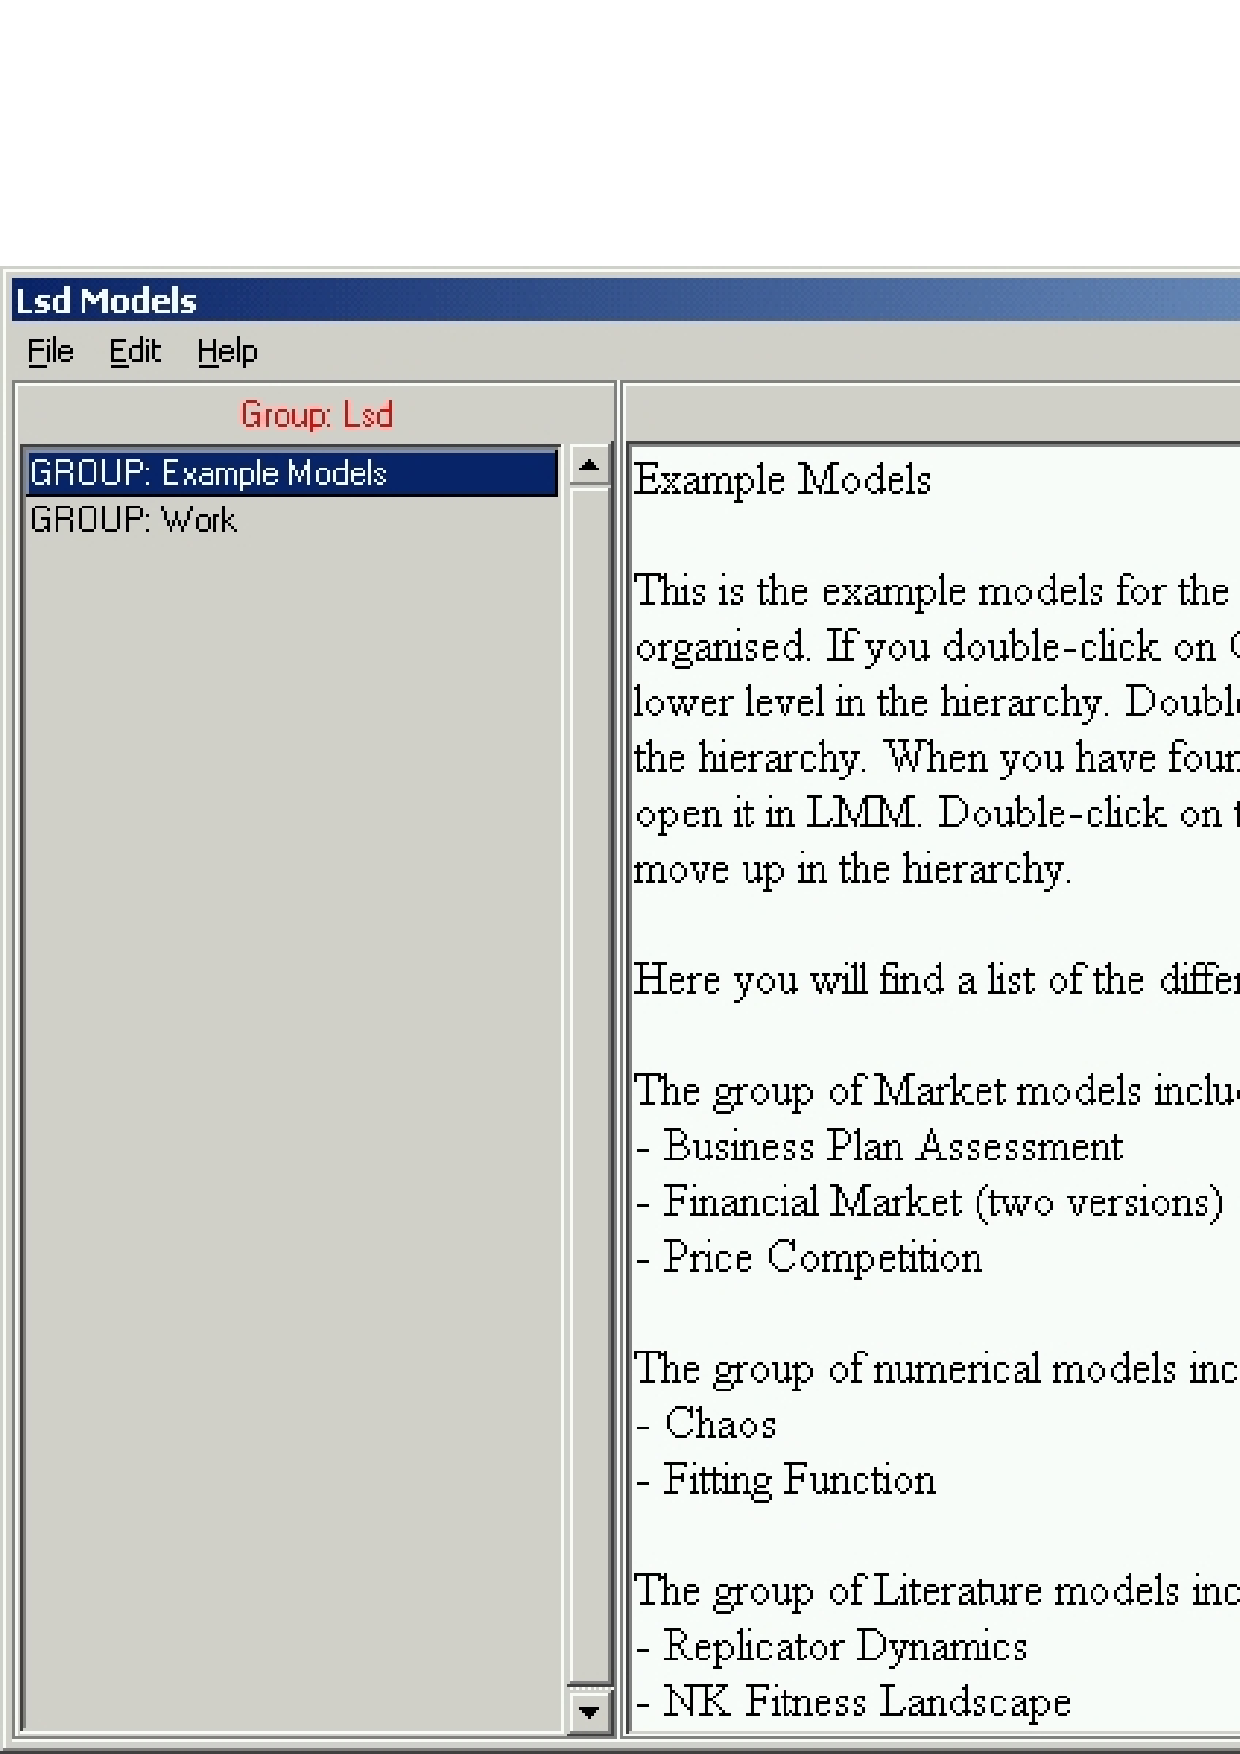
\includegraphics[width=15cm]{modelbrowser.pdf}}
  \caption{\LsD Model Manager - Model Browser}
  \label{fig:LMMbrowser}
\end{figure}

This browser shows the models available in the current \LsD installation and permits to create the structure of new ones.
Models are contained in single directories, which can be located in ``groups'' containing
related models. The Model Browser allows to navigate through the installed models:
clicking on the label of a group the browser shows the content of that group. Clicking on
the label for a model, that model is selected.

The browser' menu \menu{Edit} permits to create models or groups, to copy models from one group
to another (or to the same group with a different name), and to delete models.

The distribution includes two major groups: the ``Example Models'' group, containing
several models of different types, and a ``Work'' directory. While exploring the distributed
models you can read a brief description of the models. If you select one of the model,
LMM quits the browser and is ready to work with that model. In case you want to use
another model, in the menu \menu{Model/Browse Models} in the LMM menu bar, you can
access again the models' browser\footnote{A copy of LMM can manage only one model per time. It is possible to run multiple copies of LMM to work in parallel on two different models (e.g. to copy code from one model into another one).}. 

To quit the Model Browser you can: select one of the existing models and double-click on its name (or pressing enter on the keyboard when highlighted); generate a new model, using the model browser menu \menu{Edit/New Model}; simply exiting (key \menu{Esc}). As exercise, select a model, for example, the model ``Linear Growth'' model, stored in group ``Example Models/Exercises''.

When opening an existing model LMM shows initially a text file supposed to contain a verbal description of the model (see figure \ref{fig:LMM}). The LMM appearance is that of a standard editor, but for the menu \menu{Model} and for a
header below the menu bar.

\begin{figure}[ht]
  \centering
 \fbox{\includegraphics[width=15cm]{LMM.pdf}}
  \caption{\LsD Model Manager}
  \label{fig:LMM}
\end{figure}

The header of the LMM window shows the group containing the model, model name and its version
number\footnote{The version number of a model is used only to distinguish models. Two
models with the same name and different ver. number are completely independent, although
presumably the one with the higher version has been developed after the other one.}, and
the file currently loaded in LMM. The last element of the header shows the line and
column position of the cursor in the editor.

The menu \menu{File} deals with the text files loaded into the editor. Menu \menu{Edit},
besides the usual commands, contains several functions particularly useful when writing
C++ and \LsD code.  Menu \menu{Model} allows users to issue any command related to \LsD
model programs. Finally, menu \menu{Help} gives access to pages of the LMM manual,
which is written as a set of standard HTML pages connected with hyper-links. 

Notice that most of the entries in the menus are endowed with shortcuts, so that it is possible (and
much faster) to activate the corresponding command using the keyboard rather than the mouse. Moreover, the
secondary button of the mouse (usually the right one) clicked on the LMM editing windows
opens a short menu for frequently used commands. To get the documentation concerning a
specific command open the LMM manual page and follow the link to the command.


\chapter{Example 1 - Random Walk}\label{sec:usex}

In order to start familiarizing with the interfaces for \LsD, this section describes how to use an existing model, ignoring the task of coding the computational part of a model. Using the code written by a modeller it is possible to run pre-configured simulations, analysing the results and editing the configuration to generate new results. The example will also show a particular feature of \LsD, due to the separation of the computational part of a model (its equations) from its structural part (objects, variables, etc.). In particular, we will see that  the same computational content can be re-used in different models by simply changing the configurations. The independency of computational content from the rest of a model definition allows different data structures (containing always the same variables) to generate a variety of models.


\section{Random walk}

Let's start by analysing an extremely simple model, composed by two equations only:
\begin{eqnarray*}
X_t & = & X_{t-1} + R_{t} \\
R_{t} & = & U(min, Max)
\end{eqnarray*}


where $U(min, max)$ is a function producing a random value in the specified range with a uniform  probability distribution. Variable $X$ is called a random walk, since it makes steps in random directions, but the cumulated effects of the past generates the umpredictability of the final point of the process for large $t$'s. This variable is a good representation of many economic phenomena, mixing random events with a ``memory'' of past ones. We will play with the code for this equation observing how different configurations can exploit the same computational content expressed, as the norm in \LsD, in a general format.

The actual content of a \LsD model is divided in two parts. A so-called \textit{equation file} contains the computational content of the model, expressed as one block of code for each variable of the model. One or more other files contain  \textit{configuration}s of models, describing every other piece of information required to define a model: the elements used, initial values, number of steps, etc. The equation files must be compiled into a \LsD model program, which is a stand-alone program with the ability to perform the computations contained in the equations and can generate and use the configuration files to produce simulation runs. LMM is the a program that permits users to write the equations (or use existing equation files) and compiles the \LsD model programs. In this exercise we will use the same set of equations, and therefore the same \LsD model program. However, loading different configuration files we will actually produce simulations for different models, highlighting the power of \LsD stemming from the separation of the computational content of a model from the definition of its elements.

Open LMM, clicking on the \code{run.bat} file in the \LsD root directory\footnote{Unix and MacOS users need to enter the command \code{./LMM} from a terminal or click on its icon contained in the \LsD installation directory.} A small window will offer three options. Choose to browse existing models, go in the group \menu{Example Models/Manual} and select the model \menu{Random Walk}. The LMM editor will present a description file, used by the modeller to summarize the content of the model. 

Curious readers may want to observe the equation file, though this is not necessary. In fact, any model in \LsD is managed by LMM, that ``knows'' how the equation file is called and can therefore generate the \LsD model program containing the equations. Using the LMM menu entry \menu{Run/Show equations} the editor will show the equations. Note that the code of a \LsD model is composed of independent equations, much like translations of the model as described above in mathematical symbols and labels. One equation must be considered as the general capacity to execute certain operations, and this capacity is associated to a label (all equations must therefore be given unique labels). Each block is independent from the others, and the relative positions of the blocks (being upper or lower in the equation file) is not relevant for the results produced\footnote{Programmers with experience of standard programming languages feel usually unease about the impossibility to define elements and determine a the sequence of operation in their code. \LsD major power is actually its capacity to generate automatically the implicit information missing from explicit declarations, as the exercises in this paragraph will show.}.

In the LMM window use menu \menu{Model/Run model} to compile and run the \LsD model program for this model, and the \LsD model program will appear\footnote{The very first time a \LsD distribution is used, this procedure (the compilation) can take a minute or so, since any part of the \LsD model program must be compiled. Any subsequent generation of a model will instead be very fast, since the compiler will re-use the compiled code of the system, limiting to compile only the equations for the model.} . The LMM window in the background can be ignored as long as we are working with this model, since all operations on the model not concerning the editing of the equations are performed using the \LsD model program: definition of the model entities, initialization, running simulations etc. All the information required to start a simulation is saved in files, called configuration files (extension \texttt{.lsd}), that can be loaded into a \LsD model program to re-create a simulation run.

Any \LsD model program has the same appearance, with a window called ``browser'' and a ``log'' window. The latter window is used only to pass messages from the system to the user and control the simulation while it runs (e.g. interrupting or stopping a simulation). We will mostly ignore the log window, since the simulations for such a simple model are too fast to allow for any intervention at run time.


A \LsD model is presented by an interface based on \LsD objects, the browser. The browser constantly shows the content of one type of object, to which any command refers to (e.g. add a new variable, or set the initial values). When the \LsD model program is just opened the \LsD browser shows the only object necessarily present in any \LsD model, called \lsd{Root}. Any other object must be located as descending from (that is, contained into) this object, or one of its descendants. The browser shows the content of an object, that is, its variables (and other elements, as parameters), on the left-hand list, and objects, on the right-hand list. The menus on the top of the browser allow to pass commands to the \LsD model program.

A \LsD model program can load any configuration, although it can execute only simulation runs using the equations with which it has been compiled. In other terms, a \LsD model program cannot modify the equations it contains, but needs to be re-created to include new or modified equations. Any other aspect of a simulation besides the equation is instead defined, observed and, possibly, modified using the \LsD model program, which can store such information in so-called \textit{configuration} file. A configuration contains all the information (besides the equations), relevant to start a simulation run and manage its results. In the \LsD browser use menu \menu{File/Load} to load a configuration\footnote{Users may exploit the keyboard shortcut \menu{Ctrl+l}\footnotesize. All the frequently used commands are associated to a shortcuts withg keyboard keys. With practice, using the keyboard instead of the mouse and menus is far more efficient.}. There are many configuration files in the model directory; choose the file \menu{Sim1.lsd}. 

When a configuration is loaded into a \LsD model program a new window appears. It provides a graphical representation of the objects' structure of the model, and is endowed with features for investigating the model. As you can see the model structure of the presently loaded configuration is composed by only one type of object\footnote{The graphical representation does never contain the compulsory object \lsd{Root}.}, called \lsd{Obj1}. Also, the browser shows that the object \lsd{Root} containing the object \lsd{Obj1}. Double-click on the symbol for this new object on the graphical representation, or use the arrow keys to highlight the object in the browser and press \menu{Enter} with the keyboard. The browser will now show the content of this object, instead of \lsd{Root}, as shown by the label of the object in the browser, which reports also the name (\menu{Root}) of the object containing it. The object \lsd{Obj1} contains four entries in the list of its ``variables'': two actual variables (\menu{X (Var. lag=1)} and \menu{RandomEvent (Var. lag=0)}) and two parameters \menu{minX (Param)} and \menu{maxX (Param)}. These lines report the labels of the elements in the object and their nature. The first variable is defined as retaining data computed during a run for one time step (lag=1), because they are necessary to make computations in the following time step. As for the code of the equations, the order in which the elements are stored in the object has no effect on the results produced, which depends only on the ``logic'' of the model. For example, you may notice that variable \lsd{X} appears in the list before variable \lsd{RandomEvent}, although the value of the latter must be computed before the execution of the equation for the former. \LsD model programs systematically arrange the order of the variables so that the computations will take place in the appropriate order\footnote{Modelling the order of execution of the different routines in a simulation program is a difficult task, and it is particularly difficult to modify such order in large models. One of the main advantages of \LsD is that this order is automatically generated at any moment, with the system controlling for inconsistencies or issuing information as required. Still, modeller can, if relevant, fix a specific ordering for the equations.}. 

Besides the objects and the other elements (variables and parameters), the configuration contains also the information required to start a simulation, like the initial values, number of steps, etc. Therefore, once a configuration is loaded into a \LsD model program we are ready to start a simulation run. Choose menu entry \menu{Run/Run}, and a summary window will appear. The window warns that any simulation run overwrites the existing configuration file. Since we did not change anything in the configuration, this will simply re-create the same configuration file we just loaded. Press \menu{Ok} and the simulation will start, lasting some fractions of a second. During this simulation run the only information provided is the sequence of time steps completed. As we will see, it is possible to change the information provided at run time either setting the options in the configuration or using the log window to pass commands to the system. 

\section{Analysing the results}

At the end of a simulation run the \LsD model program has exactly the same appearance as before running the simulation exercise. However, there are two (hidden) differences. Firstly, the states of the elements in the model (i.e. their value) are those concerning the final time step of the simulation, while before running the simulation they referred to a conventional time $t=0$, preceding the start of a simulation run. The states of the model contained in the browser (e.g. the initial or final one) may be observed, and even used as initial states for a new simulation run, though we ignore this possibility now. 

The second hidden difference of the \LsD model program is that it has retained some of the data generated during a simulation run. Which series must be saved from a simulation, and which must instead be discarded at run time is another option that users can set, and is stored in the configuration. This is due to the fact that many large models can easily be computed in reasonable times, but the data generated are so many that there is no memory is large enough to store all the series, and therefore users must select which series to use\footnote{The system produces a warning when the operative system is not able to supply the memory required to store the data selected.}. 

To access the data saved during the simulation run we need to use the module Analysis of Results. Access this module using menu \menu{Data/Analysis of Results}. The browser will be replaced by a new window containing three list boxes\footnote{In case the module is launched before running a simulation, then it will be empty, and a warning will appear listing the possible causes and the possibilities for the module to load data other than from just executed simulation runs.}: the data available from the latest simulation run (\menu{Series Available}); the list containing the series one wants to process (\menu{Series Selected}); the list of the graphs generated in the session of analysis (\menu{Graphs}). In the present case, the module contains only one series, for variable \lsd{X}, indicated with a line containing: its label, a progressive value (1) and indicating the time steps available for the series (from time 0 to time 1000). Notice that the data for the other variable \lsd{RandomEvent}, as well as for the parameters are not available, indicating that the configuration specified that only the data produced by \lsd{X} had to be retained\footnote{\LsD treats the data produced by variables identically as those contained by parameters, so that even the latter can, if relevant, be used in the analysis of results, although it generally makes little sense. In some cases, however, models may be implemented in such way to modify the values of parameters, turning them, in effect, into variables.}.

The use of the analysis module is rather straightforward. Highlight the series available, and press the button \menu{$>$} (or double-click on the series). The series' label is now copied in the central list, and the data it refers to can be used for various analyses. There are many options to generate many different types of graphs. Leaving the default options, the module generates \menu{Time series} graphs (using the data stored across time steps for the selected series) and \menu{Sequence} analysis, using the data in ordered series. The two options together generate therefore a graph using the temporal sequence of the data contained in the series selected. Leave the options as they are, press button \menu{Plot} on the bottom-left corner of the window.

A new window will appear, containing the graph of the (only) series selected (and a new entry will appear in the list of graphs in the main module's window). The graph window shows the time on the horizontal axis and represents with a line the values of the series selected. The pattern of the line is a typical graph for a random walk variable. The graph windows have several features useful to manage their content and favor the analysis of simulation results. For example, the window my be double-clicked to push it in the background. Clicking on the graph's entry in the \menu{Graph} list brings it again in the foreground. Moving the mouse over the graph window will show the coordinates of the mouse pointer in the bottom part of the window. 

\section{Managing random events}

The model we generated uses random events, and a typical issue concerning simulations involving random events consists in testing for the robustness of the results. That is, we want to know whether a give result is due only to a particular combination of random values, or, instead, it is always generated independently from the random values used. Exit from the analysis of results module (menu \menu{Exit}, or press the key \menu{Esc} and confirm), and you will have again the browser. As mentioned before, the state of the model contained the browser is not the state as contained in the configuration file we loaded before, but the state of the model at the end of the simulation run. Attempting to run a simulation now, with the browser containing the final state of a previous simulation run, will cause an error, preventing the actual start of the simulation. Try to use the command \menu{Run/Run} and the error message will explain the type of error.

The problem is that just before starting to compute the simulation steps the \LsD model program writes a configuration file containing the state of the model. This is necessary because users must be able to replicate any simulation result produced. Running a simulation with a configuration representing the final state of a model is obviously different from re-running the same simulation with the configuration stored in the file. If the user really wants to continue a previous simulation run, then it is necessary to explicitly save the final state as a new configuration, which can then be loaded and used for a simulation run. Instead, willing to replicate a previously computed simulation it is necessary to re-load the same (original) configuration. You can do this using the command in menu \menu{File/Reload}. After this command (as after loading any configuration), it is possible to run a new simulation using exactly the same configuration used previously. Ensure that you have loaded in the browser the fresh configuration, using either the reload command or the load command, and indicating again the \menu{Sim1.lsd} configuration file.

Run again the same simulation, and after that re-open the module analysis of results (\menu{Data/Analysis of Results}) to generate again the time sequential graph of the \lsd{X} variable, following the same steps we used before. The graph will be identical to the one previously obtained. This means that the random events used, though having all the properties of a random variable, are not actually stochastic. In fact, programming languages (and obviously also \LsD) uses a so called \textit{pseudo}-random generator. These are deterministic routines that return different values any time they are used, and these values have a distribution with the probabilistic properties of a real random function. It is possible to reset the pseudo-random generator to force it to repeat the same series of (pseudo-)random values, as we implicitly did re-launching the same configuration. Obviously, it is possible to set the generator so that to create new (pseudo-)random series. Each series of values produced by the random number generator is associated to a value, called \textit{seed}, that is part of the configuration and can be set by the user as part of the simulation setting in menu \menu{Run/Sim.Settings}.

Our goal of testing for robustness cannot therefore be fulfilled, since we used exactly the same random values. \LsD offers at least two options for this objective, as will be discussed in the following paragraph.

\section{Multiple objects}

One of the most useful features of simulations is that you define once a model, and then you can replicate its results many times, in effect generating many ``virtual histories'' to be studied, for example, to appreciate general properties of the modelled system\footnote{Or, as suggested in the methodological part, in order to individuate the conditions that give rise to rare, but relevant, events.}.

\LsD allows users to execute many runs sequentially, generating results for each of them using different seeds. The results from each run will be saved in files, that can then be loaded into the analysis of results module for comparison. However, this simulative technique is almost always not efficient. Running sequentially many simulations for small models, requiring little memory and computational time, means to occupy most of the CPU time to load a configuration and saving results on file. Furthermore, you will flush your disk with as many files as simulation runs you need, a number that can easily reach the thousands. Much more efficient is to run many simulations in parallel if, as in our case, the memory requirements are negligible.

Load the configuration file \menu{Sim2.lsd}. This configuration is identical to that used before, but for the fact that it contains 10 copies of object \lsd{Obj1}, each containing a copy of the elements defined within this object. Run the simulation and open the analysis of results module. Now you will find 10 different series, each of them representing a random walk series. You can double-click on each series and produce a graph for a single series, or select a group or all them and generate a single graph with multiple series.


All the series are independent from one another, though using the same initial values. In effect, this configuration represents a model that may be expressed, using the conventional indexing system, as:

\[
X^i_t=X^i_{t-1} + U(min^i, max^i)
\]

where $i=\{1, 2, ..., 10\}$. The \LsD representation of models does not make use of indexes, but of objects, though the meaning of the two formats is obviously identical. When we use the traditional vector-based representation, indicating with the same index $i$ two elements means that they are somehow connected, and should be used together. In \LsD instead we define objects: elements contained in the same copy of a given type of object have the same relation as if they were sharing the same index in a vectorial expression.

It is worth to note that the language for writing the \LsD equations does not make use of indexes, but uses only the labels of elements, without specifying which copies should be used. This format has the potential ambiguity that the code does not specify where the elements required to compute an equation should be taken from. For example, when the equation computes the value for variable \lsd{RandomEvent} contained in the first object (say, with $i=1$), the code does not indicate where is located the parameter \lsd{minX} necessary for its computation. The system contains 10 different copies for this parameter, and therefore, each of these copies may be, in theory, used. This potential ambiguity is solved by \LsD using the structure of the model, that is, the relations among objects and the elements contained there. The first rule applied by \LsD is that an equation requires an element, firstly search for the element within the same object. Consequently, every \lsd{RandomEvent} in the model will be computed using the copy of \lsd{minX} in the same object.

\section{\LsD automatic data retrieving}
One of the most powerful features of \LsD is that the system automatically interprets the code \textit{and} the state of the model in order to determine which operation needs to be done at any moment of the simulation run. For example, we already noted that the order of execution of the equations is automatically generated by the system, so that there is no need to place in particular order the code for the equations of the variables' declaration. We see now another advantage of the \LsD way to express models.

Load the configuration \menu{Sim3.lsd}. Though the equations are obviously identical (they are coded into the \LsD model program and cannot be modified by the program itself), this configuration differs from the previous ones, including an additional object, \lsd{Obj2}, contained in \lsd{Obj1}. Looking at the content of the objects you can see that the same elements we had before in one single objects are now divided between the two objects:  \lsd{minX} and \lsd{maxX} remain in \lsd{Obj1}, while the two variables have moved to \lsd{Obj2}. As indicated by the graphical representation, there are 10 copies of \lsd{Obj2} contained in a single copy of \lsd{Obj1}. Therefore, there is only one copy each for \lsd{minX} and \lsd{maxX}, and 10 copies for the two variables.

Changing the model structure, we, in effect, computed a slightly different model, which may be expressed, using the conventional vector-based expression, as:

\[
X^i_t=X^i_{t-1} + U(min, max)
\]

where $i=\{1, 2, ..., 10\}$ refers to the different copies of \lsd{Obj2}, and the two parameters are common for all the \lsd{X}'s in the model. The two parameters have no need to be assigned any index since there is only single copy for each of them. 

Run the simulation for this configuration: it will produce results identical to those produced with \menu{Sim2.lsd}. Since all the copies of \lsd{minX} and \lsd{maxX} in configuration \menu{Sim2.lsd} where identical, it is not surprising that the results are the same. What is surprising, from the computational perspective, is that the model equations can indifferently compute both models. The reason is the second rule used by \LsD to retrieve values while computing the equations: if an element is required but it is not found in the object of the computing variable (in our example, \lsd{minX} is not found in \lsd{Obj2} where \lsd{X} is stored), then scan all the model structure to find it.

Using an object-based expression rather than a vector-based one provides huge advantages. For example, we can limit the number of parameters, sharing the same copy of an element though it is used for many different equations. Once a modeller gets used to this expression, it is much easier to build a model as an imitation of a real-world system, particularly when implementing agent-based models. As we will see, the equations' language requires the modeller to express only the computational content, referring to the elements of the model only by their label, and not using indexes or other ways to identify the location of the elements. It is the hierarchical structure of the model that guides the search for a specific element.

To better appreciate how \LsD exploits the model structure to identify the elements to use for a simulation, load the configuration \menu{Sim4.lsd}. As you can see, the model structure is identical as in \menu{Sim3.lsd}, but for the fact that we have now two copies of \lsd{Obj1}. The structure of the two copies are identical, that is, they contain the same parameters, variables and descending objects. In \LsD elements with the same labels are constrained to have the same structure. However, they can contain different numerical initialization. In this example, both groups of objects \lsd{Obj2} are composed by 10 copies, but the values of the parameters in \lsd{Obj1} are different (-10 and 10, for the first copy, and -1 and 1 for the second).

Now the model computed is yet another version:

\[
X^{i,j}_t=X^{i,j}i_{t-1} + U(min_j, max_j)
\]

where the index $j=\{1,2\}$ refers to the copy of \lsd{Obj1}.

Run the simulation and observe the results. The 20 copies of variable \lsd{X} are now identified by two digits, the first for the copy of \lsd{Obj1} and the second for the copy of \lsd{Obj2}. As you will see, plotting the two groups of variables, the groups of series span over different ranges, reflecting the different values of the parameters used.




\section{Functions vs variables}
\LsD provides users with two elements that can generate computations: variables and functions. Variables, as those used in the model configuration so far, are elements that execute their equation always once and only once at each time step, assuming the resulting value as their state for the concerned time. The system ensures that each variable is updated at each time step and that the appropriate values in their code are used. For example, if a variable's value is used in the code of many elements of the model within a single time step, its equation is executed only once (the first time its new value is requested), while the any subsequent request of its value within the same time step returns the same value without re-executing the equations' code. 

Functions are similar to variables, but their equations are executed only, and every time, their values are requested by the code in other equations, independently from the time step. In effects, functions do not have a value for each time step, since at any time $t$ they may produce many different values, or none, depending on how many times they have been requested by other elements in that time step. 


To appreciate how functions work load the configuration \menu{Sim5.lsd}. This configuration is identical to \menu{Sim4.lsd} but for the element \lsd{RandomEvent}. In the previous configurations  this element is defined as a variable, computed once and only once, and whose values are used only by the copies of variable \lsd{X} located in the same copy of \lsd{Obj2}. Now, instead, we find \lsd{RandomEvent} defined as functions (and not variables) located in \lsd{Obj1}. If you ran the simulation you will obtain exactly the same result as those produced by \menu{Sim4.lsd}, though by means of a different computational structure. Every copy of \lsd{X} will make use of the copy of \lsd{RandomEvent} contained in its \textit{parent} object. Moreover, every \lsd{RandomEvent} will be computed many times in the same time steps, reporting different values to the different copies of \lsd{X} requesting its value.

Functions can be thought of as pieces of code generating values that have no relevance, \textit{per se}, as simulation results, but need to be computed occasionally by other elements in the model, at times independent from the simulation steps. For example, a function may contain the code to express the entry of a new firm in a market, if the entry is a rare event. The entry may be triggered by many different events (e.g. an incumbent's spin-off, innovation, etc.) but each of them would produce the same initialization code contained in the function.

The existence of functions permits to express \textit{event driven} models, as opposed to \textit{time driven} ones. An event-driven model is made of functions that trigger one another in a cascade of computations. \LsD offers the opportunity to integrate the two modelling styles, where, for example, variables (i.e. time driven computations) deal with data collection and management, while the core of the model is expressed by functions.

  
\section{Analysing massive amounts of data}

\LsD is particularly suited to generate and analyse data from very large models. Since \LsD is, in effect, made of C++ code, a model can easily exploit all the computational power made available by the hardware. For very large models, however, the management of large amount of data is more problematic than their generation. This is due to the fact that modern processors can easily generate massive amount of data that necessarily require specific tools to be stored and analysed. \LsD offers flexible and highly efficient tools to deal not only with single series, but also to manage whole batches of data generated in simulations of very large models.

As an example, load the configuration \menu{Sim6.lsd}. It is the same configuration as \menu{Sim3.lsd}, but the number of \lsd{Obj2} copies are set to 10,000. Run the simulation (it will be slower than before, lasting about 10 seconds) and you will produce as many series, each containing 1,000 data, for each of the time step executed.

Opening the module for analysing the results your will have a huge number of series.  The first problem caused by large amounts of data is due to the simple selection of the series we want to work on. Clicking on each series individually is obviously out of question. It is possible, though time consuming, to use other selection mechanisms embedded in the list-box, like clicking on the first and then last series while keeping the key \menu{Shift} pressed. Still, the selection of data within a large data set is problematic, particularly for models with several types of series saved.

The \LsD module for analysing results is designed to facilitate the management of large amounts of data. Concerning the selection of the series, for example, it is possible to pass the system several types of criteria for selection. Click with the right button of the mouse any of the available series. A new window will offer several systems to select a whole group, or batch, of series, depending on different criteria. The options available are rather sophisticated, though, hardly viable for our simple model. Use the default option (\menu{Select all the series}), and confirm. All the series will be immediately moved into the central list.

Though it is technically possible to plot the time pattern for all the series, this is practically impossible, and rather meaningless. In fact, the limitation is due to the computational costs of generating 10 million points in the graph individually, as required by such a graph. Moreover, when using large models we normally are not interested in observing so many series through time, but are rather interested in the assessing global properties at a certain instant of time, for example at the end of the simulation run. To do this, select the option \menu{Cross section} instead of the default \menu{Time series}. 

The graph produced with this option will consider as a single sequence all the data from different series at the same time step, where the series appear on the horizontal axis. Such graph requires additional information since it can be customized in several ways. For example, it is possible to generate many series corresponding to different time steps. Also, the order in which the series appear on the horizontal axis can be changed reflecting the values of the series at a specific time. 

 After clicking on the button \menu{Plot} the system will show a new window, where you need to enter the time step(s) to use. By default the window offers the latest time step available. Click on \menu{Add}, and the time step will be added to the list of time steps to use. Press then the button \menu{Continue} to generate the graph. The new graph window will report a single line referring to the time step inserted (1,000) using values for all the 10,000 series that appear on the X axis according to their ranking in the list-box. 

The graph is actually quite meaningless. In fact, each series is represented on the horizontal axis in a position determined by its order of appearance in the selected list box. Since these series are independent, there is no particular order in the values shown in the graph. To make sense of these values, we can organize the order of the series on the horizontal axis according to some criterion. For example, ordering them for decreasing values, as reported at the chosen time step.

Press again the plot button, and insert as before the last time step. However, before pressing on \menu{Continue}, click on the button \menu{Sort Descending}. The insertion window will report that the series will be re-organized according to the descending values at the specified time step. Confirming the options chosen, you will now have a more orderly graph. Though the random walk dynamics are known to have infinite variance as time increases to infinite, at a given time they have a known distribution. Our simulation can be interpreted as a sample of 10,000 independent random walks, and therefore we can expect them to distribute according to density of the underlying probability function. The graph shown that there is a small number of very high and very low values, and larger number of intermediate results.

The cross section graphs report the values for the series, from which we may induce, but not observe, the actual frequencies. \LsD allows also to generate frequency classes from the data selected. Always having all the series in the central listbox, and keeping the option \menu{Cross section} selected, click on the button \menu{Histograms}. Again, being a cross section, you will be asked for the time step to use (leave the default value). Also, the window will ask for the number of classes. Insert in this latter cell the value of 20, and press \menu{Ok}. The graph will report 20 columns with the same width. On the horizontal axis the graph reports the range of the sequence used (the values of \lsd{X}'s at the last time step). The range is determined by the maximum and minimum values of the series used, divided evenly in as many classes as specified. The resulting segments are used as the bases for the histograms, whose height is proportional to the number of series taking a value falling in the interval of the class at the specified time step. The vertical axis reports both the absolute frequencies (i.e. the number of series in the class) and the relative percentage. Moving the pointer of the mouse on the boxes will provide information on the class, like its intervals, middle value, actual average value of the values contained etc.

You can generate new histograms, using different class numbers and using the other options (see the \menu{Help} if necessary). The distribution will clearly be a symmetric one, strongly resembling a normal distribution function.






\part{Tutorials}\label{ch:tutorials}
\chapter{Implementing \LsD models: Example 1}\label{sec:tut1}

Implementing a simulation model for research purposes is a process prone to errors. We can divide the possible errors in two classes. Firstly, we may simply write the wrong code or values, so that the model implemented is different from the one we wanted to implement. Secondly, we may discover that, though implementing the model we originally designed, it is not appropriate for the purposes of our research, and therefore we need to modify the original idea. 

In either case, an error needs to be firstly spotted and then fixed. Identifying an error can be very difficult: a large model, with dozens of routines and thousands of variables produces massive amounts of data, that are likely to be analysed only statistically, at aggregate level. Unless the error generates evident absurdities (say, negative market shares), it is well possible that the faulty code goes unnoticed. 

Even in the case we identify an error and the required solution, say, replacing the code for a variable, the effects on the rest of the model may be huge, producing an avalanche of further changes on the rest of the model forcing, in practice, a complete re-writing of the whole model.

\LsD provides very powerful tools to assist users in both respects. \LsD models are automatically endowed with a large series of interfaces to access the state of the model in many different ways, facilitating the identification of problematic code. Also, the very structure of a \LsD model is made of independent chunks of code, minimising the possibility that a few changes require the re-writing of large portions of the model. Still, even though \LsD allows technically to find and fix problems at any stage of a model development, it is far easier to adjust a model

In both cases, it is good practice (and, in many case, of capital importance for the success of a project), to develop the model gradually, adding few element at a time, testing the (theoretically trivial) intermediate results, and proceed adding further complications. Without this approach, implementing at a single stroke hundreds of lines of code and dozens of values, we can be guaranteed to generate a long list of errors, whose combined effect make practically impossible to identify their original source. Moreover, even in case we managed to generate an error-free model, we are likely trapped in the black-box problem, since we cannot trace the properties of the results to the specific assumptions implemented in the model definition. In this section we will build a model step-by-step, so to have the possibility to discuss any aspect of modelling with \LsD. 

In this section we implement from the scratch a new model, which eventually will represent a discrete version of the replicator dynamics model. The process of model construction will be described step-by-step, with the aim of familiarizing readers with the major interfaces and operations. The steps described have also the purpose to show how a typical simulation project may proceed, by adding a few elements at a time, testing the results, editing the model, and extending it. As initial stage we start by implementing a model with one single variable, say $X$, computed as a random value.


\section{Create a new model project}
A \LsD model requires several files, and the user is generate more, e.g. for different configurations, results, graphics, etc. To create a model it is then necessary to create firstly a directory where to place the basic files (essentially the equation file). The various models located in an installation can be organized in \textit{groups}. The installation originally contains two groups: example models and work in progress. Users are obviously invited to place their models in the second group. Within a group the user can obviously create other groups, typically for sets of related models. Any group or model create its own directory that can be inspected, but whose content is safe not to alter unless using the LMM tools


To start the system launch we consider you already unpacked the installation file. Click on the \code{run.bat} file to start the system.\footnote{For non-Windows users is also necessary to compile the \code{lmm} file. See the instructions on the installation in this document on in the accompanying files. For these system the system is launched directly the \code{lmm} executable}.

The program starts offering automatically to open a \LsD model, with the alternatives being to use LMM as text editor. Opting to use models the system activate a model browser showing all the models present in the installation, which also permits to create new ones.\footnote{The browser can be activated, besides at the start time, by choosing the LMM command \fmenu{Model / Browse Models}.}
 
\begin{figure}[ht]
  \centering
 \fbox{\includegraphics[width=12cm]{modelbrowser1.pdf}}
  \caption{Model browser, initial screen}
  \label{fig:modelbrowser1}
\end{figure}


Using the mouse pointer or the arrow keys choose a group, e.g. ``Work in Progress'', and then uses the module's own menu \menu{Edit} and then \menu{New Model/Group}. You will have the choice between creating a new group or insert a new model. Opting for the latter you will be requested a few details to identify the model. Firstly a model name and a version number, which will be used solely to label the model for users. The third field, the directory name, needs to be a non-existing directory and cannot contain spaces, punctuations, etc.

Confirming on \menu{Ok} will create a new directory (or a warning in case of error) with all the necessary elements required for an ``empty'' \LsD model program.  The most relevant is the file that LMM will use assuming it contains the code for the equations of the model. The filename is conventionally labelled as \code{fun\_XXX.cpp}, where \code{XXX} is the model directory name. Users may change the file name, but this is potentially dangerous since LMM considers only changes to the equation file to be included in the model. 

At the end of this procedure the the LMM editor window shows the equation file for the new model. Although this is pure C++ users are invited to use keywords specifically designed to make simpler the expression of the most frequently used \LsD expressions. 

After the successful creation of the new model, LMM shows in the top bar the reference of the model (label and file name). Moreover, it automatically opens the equation file name, assuming that the user needs to start from there. The equation file name appears in the LMM editor as shown in figure \ref{fig:LMMnew}.

\begin{figure}[ht]
  \centering
 \fbox{\includegraphics[width=10cm]{LMMnew.pdf}}
  \caption{Empty equation file for a new model}
  \label{fig:LMMnew}
\end{figure}


The equation file contains at the very first line a call to include the definition of all the \LsD specific command (file \code{fun\_head.h}). The two following keywords, \code{MODELBEGIN} and \code{MODELEND}, are the markers stating the initial and final lines within which the user is allowed to insert the code for the equations. The last command, \code{close\_sim()}, can be ignored for now.\tech{In the rest of the text notes like this one will report on technical aspects, of possible interest for advanced users, but not relevant for the standard use of \LsD. \newline Many of the commands used in \LsD equations are obviously not C++, but are part of a \LsD macro language. \LsD macro language and C++ can coexist in the same equation file. For example, the \texttt{MODELBEGIN} macro declares a function (a method of a C++ class) and initialize all its local variables. If necessary,
users may add new local and/or global variables to the file. \texttt{close\_sim()} allows to perform post-simulation cleaning, like removing memory explicitly allocated during the simulation by the code written by the modeller. Obviously, all memory used by the system is automatically dealt with by the system.}


At creation the file contains no equation, but it is anyway technically sufficient  to create and
run an \LsD model program, although, obviously, without equations the \LsD model program
will not be able to execute a simulation run. 



\section{Introduction to \LsD equations}
Users define in the equations of the model all the operations that need to be executed by
the model. Equations are pieces of code are associated to a label; during a simulation run, whenever the system needs to compute the value for a variable, it passes the control of the program to the equation file. Here the system searches for the piece of code associated to the variable to be computed, and executes its lines, returning to the simulation (i.e. searching for the next variable to compute) at the end of the line of the equations for that variable. Therefore, each equation must necessarily indicate at the very least two basic elements: the name of the variable it refers to, and the final value to be used as result of the equation execution. In between is possible, of course, to place any number of intermediate lines containing legal C++/\LsD commands, typically used to elaborate the value to be returned.

If LMM is not showing the equation file, use the menu \menu{Model/Show Equations} to have LMM re-opening the equations' file. It is very important that you never open file for the equations using the menu \menu{File/Open File}. In fact, although this is not formally incorrect, there is the possibility that you edit the wrong file. In this case, the
equations' editing is not included in the \LsD model program, which keeps on using the old, un-edited, equations' file, and therefore the \LsD model program will not include them. When LMM is requested to show the equations' file it reads the name of the file used to create the \LsD model program, and therefore there is no risk of editing the wrong file.\footnote{Users can modify the name of the equation file changing the content of the compilation model options, using the relative option in menu \menu{Model}.}

Place the cursor of the LMM editor in any point of the file after the line \code{MODELBEGIN} and before \code{MODELEND}. It is now time to discover some of the utilities that make LMM very useful to write \LsD model programs. The equation file is a simple text file, so that any text can be simply typed in. However, typographical mistakes are very common and their correction time consuming. Hence, LMM offers the opportunity to activate small interfaces that ask for the model-specific information, and then automatically insert the (error-free) text for the most commonly used commands. These interfaces are called \textit{scripts} and are available for several commands, including all the variations for specific options.

\begin{figure}[ht]
  \centering
 \fbox{\includegraphics[width=7cm]{script.pdf}}
  \caption{List of the scripts available to automatically insert \LsD commands into the equation file.}
  \label{fig:script}
\end{figure}


To use a script place the cursor where you want to insert the text (in our case, anywhere in between the keywords for the start and the end of the equations, adding lines as necessary. You can then choose three different ways: menu \menu{ Edit / Insert Lsd Script}; click with the secondary (right) button of the mouse; press with two fingers the keys \code{Ctrl+i}. In any case you will be shown a list of the available scripts available, as in figure \ref{fig:script}.


In our case, we need to insert a the code for a new variable, thus select the first option in the list (or press the key \menu{e}) and press the key \menu{Return}, or click on \menu{Insert}. Notice that almost every operation necessary to write the equations can be performed \textit{without} the use of the mouse, but only using the keyboard. Getting experienced in using the keys and the available shortcuts increases dramatically the speed of typing the equations in respect of using the mouse. 
 
Following the choice of inserting a new equation you will be asked to type the name of the variable (choose \lsd{X}). Notice that focus is already in the cell for the variable name, so you just need to type the variable name. Pressing \menu{Return} the focus is shifted to the button \menu{Ok}, so another hit on the same key will conclude the script operation.

The script provides with a skeletal (and yet incomplete) code for the variable \lsd{X}. 

\small
\begin{verbatim}
EQUATION("X")
/* Comment */

RESULT( )
\end{verbatim}
\normalsize

The line \code{EQUATION("X")} marks the beginning of the equation, that is, the start of the code that any variable labelled \lsd{X} in the model will begin to execute whenever it needs to compute a value. 

The editor places the curse so as to invite you to type in the lines immediately below the header. Any test inserted in between the symbols \code{/*} and \code{*/} is considered as comment in C++ (and highlighted in green in LMM) and therefore ignored by the program. This specific comment is particular relevant, because it is considered as the ``official'' documentation for the variable, and the system will automatically use this comment here any time the documentation of the variable is requested. 

 The last line, \code{RESULT()}, indicates the end of the equation and must be assigned, within the round parentheses, the numerical value returned by the equation and assigned to the variable.

Let's write the possibly simplest equation. In between the parenthesis of the
\code{RESULT()} type the command \code{RND}. This is a \LsD command producing a different
random value drawn from a uniform random function between [0,1]. Therefore, the complete
equation's code is:

\small
\begin{verbatim}
EQUATION("X")
/*
  A uniform random value
*/

RESULT(RND)
\end{verbatim}
\normalsize

When an equation file is edited it must explicitly be saved, since the compiler does not read the editor window, but only the content of the file. Therefore, save the equation file (menu \menu{File/Save} or shortcut \menu{Ctrl+s}) and, to compile,  use menu entry \menu{Model / Compile and Run} (shortcut  \menu{Ctrl+r}). This will create (and execute) the new \LsD model program containing the new equation.

If you try to compile without saving, the system asks whether you want to continue without saving, or if your want to save the current file before compiling.

At this point LMM should show the new program just compiled (figure \ref{fig:lsdbrowser}), which is automatically launched. If the \LsD model program windows do not appear, and you have an error message instead, this means that you managed to put an error in your equation's code. Read the newly appeared \menu{Compilation Results } window for indications on the line number where the error is located. See also the appendix \ref{sec:progr_err} (pg. \pageref{sec:progr_err}) for help on fixing the error.

\section{Defining \LsD model elements}

All \LsD model programs are externally identical, because their difference consists only in the equations they embody that have any visible effect on their interfaces. The  \LsD model program we just produced is able to compute a value for a variable labelled \lsd{X}. However, this potentiality can be exploited only defining a model where an actual variable \lsd{X} is defined\footnote{Of course, it is possible to write code for variables that are not used in a simulation. These pieces of code will not have any effect on the simulation runs, since they will never be activated.}.


The \LsD Browser provides the interfaces for creating the elements of the model, but, before continuing, let's give a look at the browser.

\begin{figure}[ht]
  \centering
 \fbox{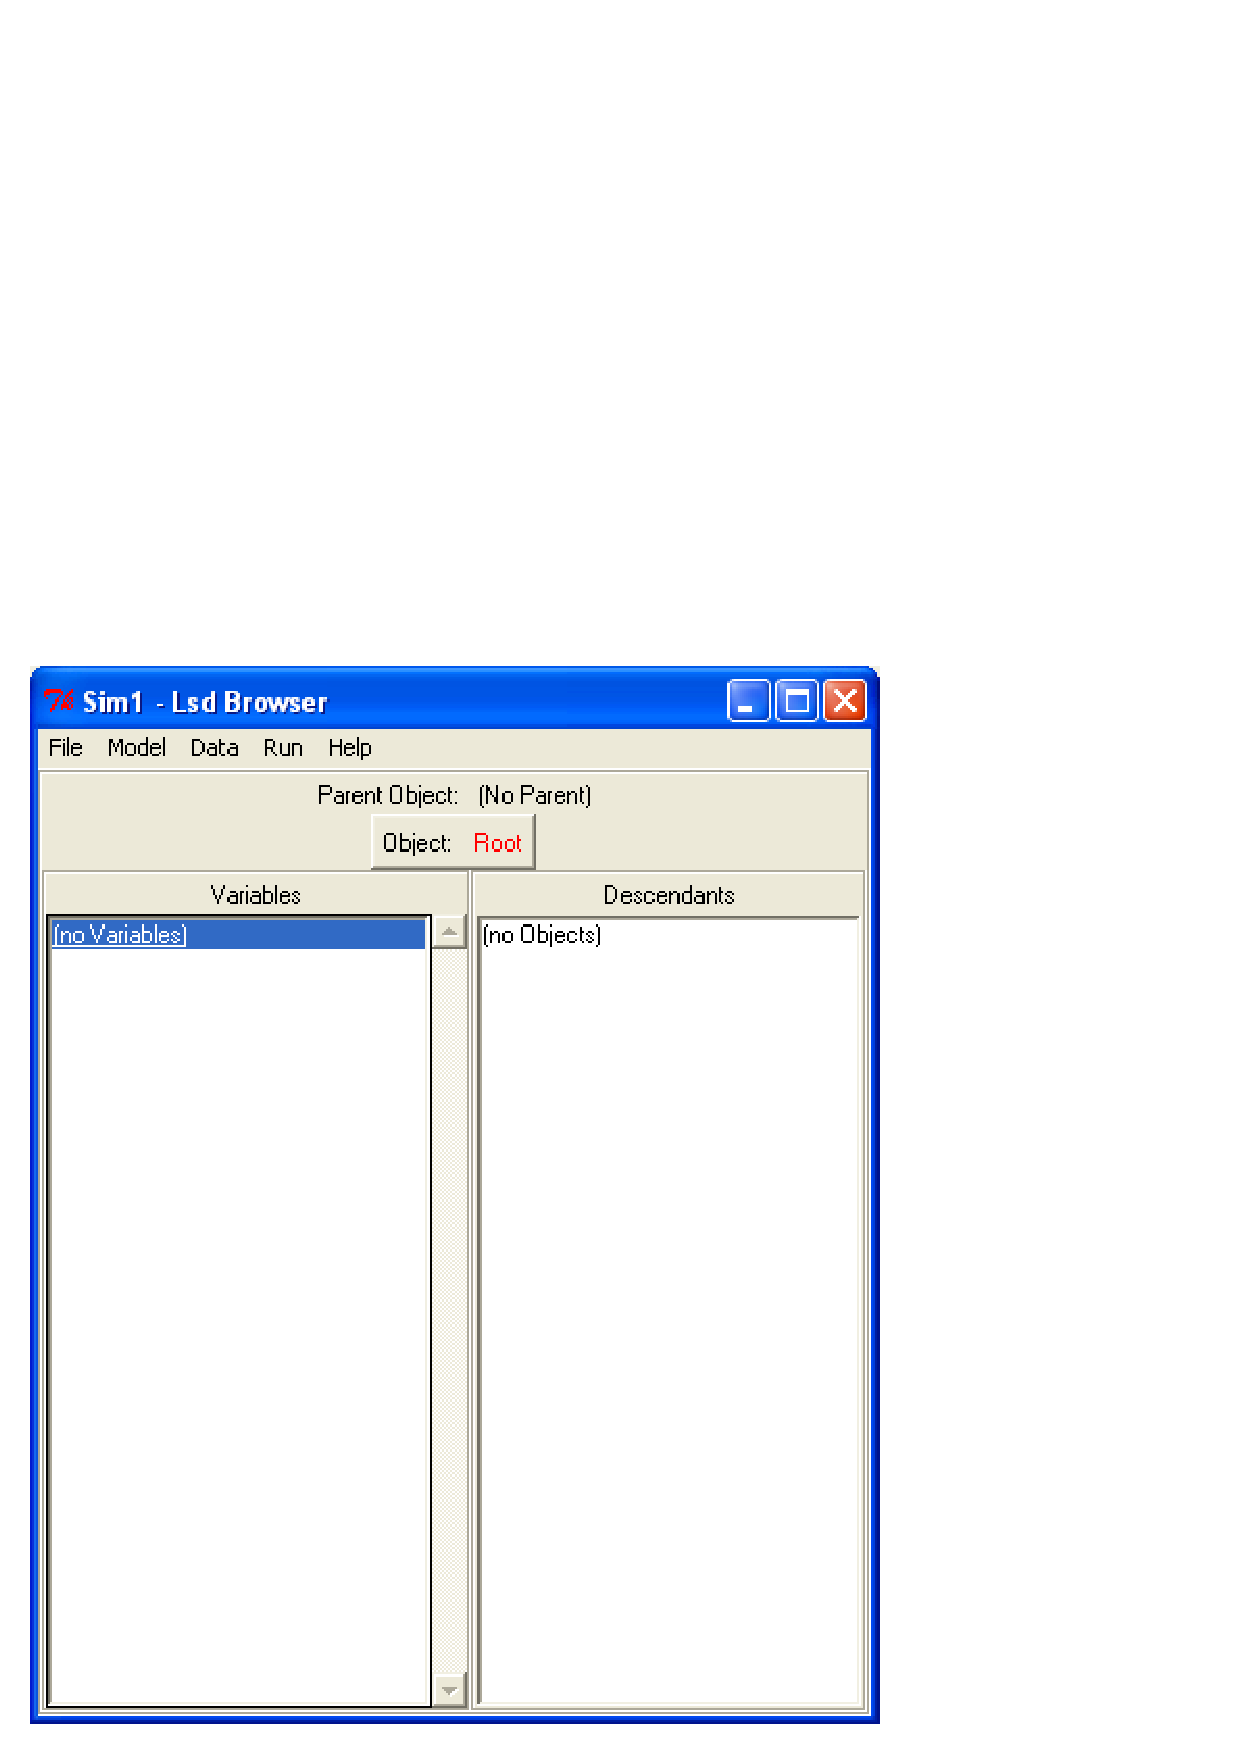
\includegraphics[width=7cm]{lsdbrowser.pdf}}
  \caption{\LsD model browser, the program embedding the equations of a specific model.}
  \label{fig:lsdbrowser}
\end{figure}





The \LsD model program browser (figure \ref{fig:lsdbrowser}) is a window showing the content of one type of object in the model and providing access to all functions of a \LsD simulation model, apart those concerning the computational content (i.e. the equations). The main part of the windows is composed of two lists, empty at the start. The one on the left shows the list of numerical elements (variables, parameters and functions) of the object pointed to by the browser. The right-hand list contains the labels of the objects contained in the object shown, again empty at the start. The only object necessarily present in any \LsD model is a slightly special one, called \lsd{Root}. This object is the only one that cannot be multiplied in multiple copies, like any other one. Moreover, it is always the first object at the beginning of a time step to be scanned in search of variables needing updating. Hence, any variable placed here will surely be the first to be computed.

Just above the lists of elements are located the name of the object shown (\menu{Object: Root}) and, one position above, the name of the object whose currently shown object descends from (none, as the \lsd{Root} is conventionally assumed to be the only object not contained in any other object).

Finally, the menu bar contains the sets of commands for the operations available: file management, model structure, setting or observing data, executing simulation runs, help.


Normally, the \lsd{Root} object should not contain any variable or parameter, but
should serve only as container for the objects implementing the model. Therefore, let's
start by creating an object descending from \lsd{Root}. Choose menu \menu{Model/Add a
Descending Obj}. In the resulting window enter the label for the object, say
\lsd{MyObj}. Now the \LsD Browser will show the \lsd{Root} object containing the
\lsd{MyObj} object. Moreover, a new graphical window appears showing the object structure
of the model below (i.e. contained into) the object \lsd{Root}. Therefore, at the moment, it shows
only one object, the just created \lsd{MyObj}.

When naming elements of \LsD models users can use any printable character, and the capitalization is relevant, so that \lsd{MyObj} is different from \lsd{myobj}. It is forbidden to use points, spaces, quotations and other word-separating characters.

Move the Browser to show the content of \lsd{MyObj}. To move the browser you have several
possibilities. You can use the mouse by double-clicking the list of descendants on the
label of the object you want to move to; you can double-click the graphical
representation of the model on the object's symbol; you can just use the arrow
keys on the \LsD browser to highlight the object you want to see and press enter when you have done. Notice
that when the Browser shows \lsd{MyObj} the parent label shows that it descends from
\lsd{Root}. You can click on this label to ``move up'' the browser showing the
\lsd{Root} again (or press the letter 'u').

Eventually, we managed to have the Browser showing the content of a just created object,
which is, obviously, empty\footnote{Be sure that the browser points to the right object. If, by mistake,
you add elements to the wrong objects it is possible to shift en element to a different object. If this is the case now, however, you better start the process from the scratch. Empty the model (menu \footnotesize{\menu{\footnotesize File}}) and create again the object.}.
 Let's add a variable to this object. Choose menu item
\menu{Model/Add a Variable}. In the resulting window type the name of the variable for
which we have an equation, \lsd{X}, and press \menu{Ok} (ignore the field 'Maximum lags
used' leaving the default value of 0). Now the Browser shows that \lsd{MyObj} contains a
variable, called \lsd{X}. The list of variables shows \menu{X (0)}; this means that
\lsd{X} is a variable (as any label followed by integer numbers). Later will see that
parameters are attached the letter \menu{(P)} and functions by letters \menu{(F)}.


The definition of a model structure (that is variable, parameters and object) is stored
in memory only. Before continuing, in order to be able to reload the model structure as
we have defined it until now, save it with menu \menu{File/Save}. By default the
configuration is assigned the name of \textbf{Sim1}, although, of course, we can assign a different file name using menu \menu{File/Save as}.


\section{Running \LsD simulations}
If you have executed all the steps described above, you can now run a simulation by
choosing menu \menu{Run/Run}. Before starting, \LsD reminds you what it is going to do,
namely running a single simulation run keeping the results in memory, and over-writing possible 
configuration files having the same name\footnote{As a rule the configuration of a model is saved in a file before executing the simulation. This avoids that possibly interesting results cannot be reproduced because one forgets the configuration that produced them. However, this rule risks overwriting previous files, hence the warning message.}. Pressing \menu{Ok} will start the simulation.

The Log window shows a message on a new line for each time step successfully completed (you will see
this only when the simulation finishes after few hundredths of seconds). At the end of
the simulation the Log window reports the total time of the simulation and a finishing
message, and the Browser reappears. Besides the lines in the Log window, there is no
other difference with the Browser before the simulation run.

In fact, \LsD has done everything we have said it to do: compute the values of \lsd{X} as a
random value. But we did not tell \LsD to save or show the results in any way, so we have
lost (almost) all of them. Actually, one single value from the simulation is still available. When \LsD
terminates a simulation run the Browser keeps the status of the simulation at the very
last time step. The only way to obtain our results is therefore to repeat the simulation,
this time using the options to save the results. 

The default option when defining a new variable is that its values need not to be stored for post-simulation analysis. Every value produced by a variable will therefore be stored in memory for the time strictly necessary to complete a time step, and then it is cancelled. This ensure that large models can be simulated without limitations due to memory constraints. Obviously, some of the data produced in a simulation can  be saved, but the modeller needs to explicitly signal which element are relevant to be saved. Thus, we need to repeat the simulation after having set the option to store all values produced through time from variable \lsd{X}.

The repeat a simulation run we need to reset the configuration stored in memory from the status at the end of the simulation run to that used at the beginning. This is necessary because \LsD prevents the direct continuation of a simulation, re-starting a run after it was completed. But since it saves any configuration before a simulation run, we can easily re-load that initial state of the model without the need to re-define the model from the scratch. To do so you may use the option \menu{File / Load} and choose the only file with the extension \code{.lsd}. Since the name of the configuration we want to load is the same as the one previously loaded, you can also use the command \menu{File / Reload} (shortcut \menu{Ctrl+w}).

Notice that you really want to continue a simulation after it ended, you can save the configuration at the end of a simulation run and load it as any other configuration. 


With a fresh configuration we can not tell the system that we want the results saved for post-simulation analysis. Move the Browser to show the object \lsd{MyObj} and double-click on the variable \lsd{X} (or use the arrow keys to highlight
and press Enter). Now the Browser is transformed as shown in fig. \ref{fig:variable}.

\begin{figure}[ht]
  \centering
 \fbox{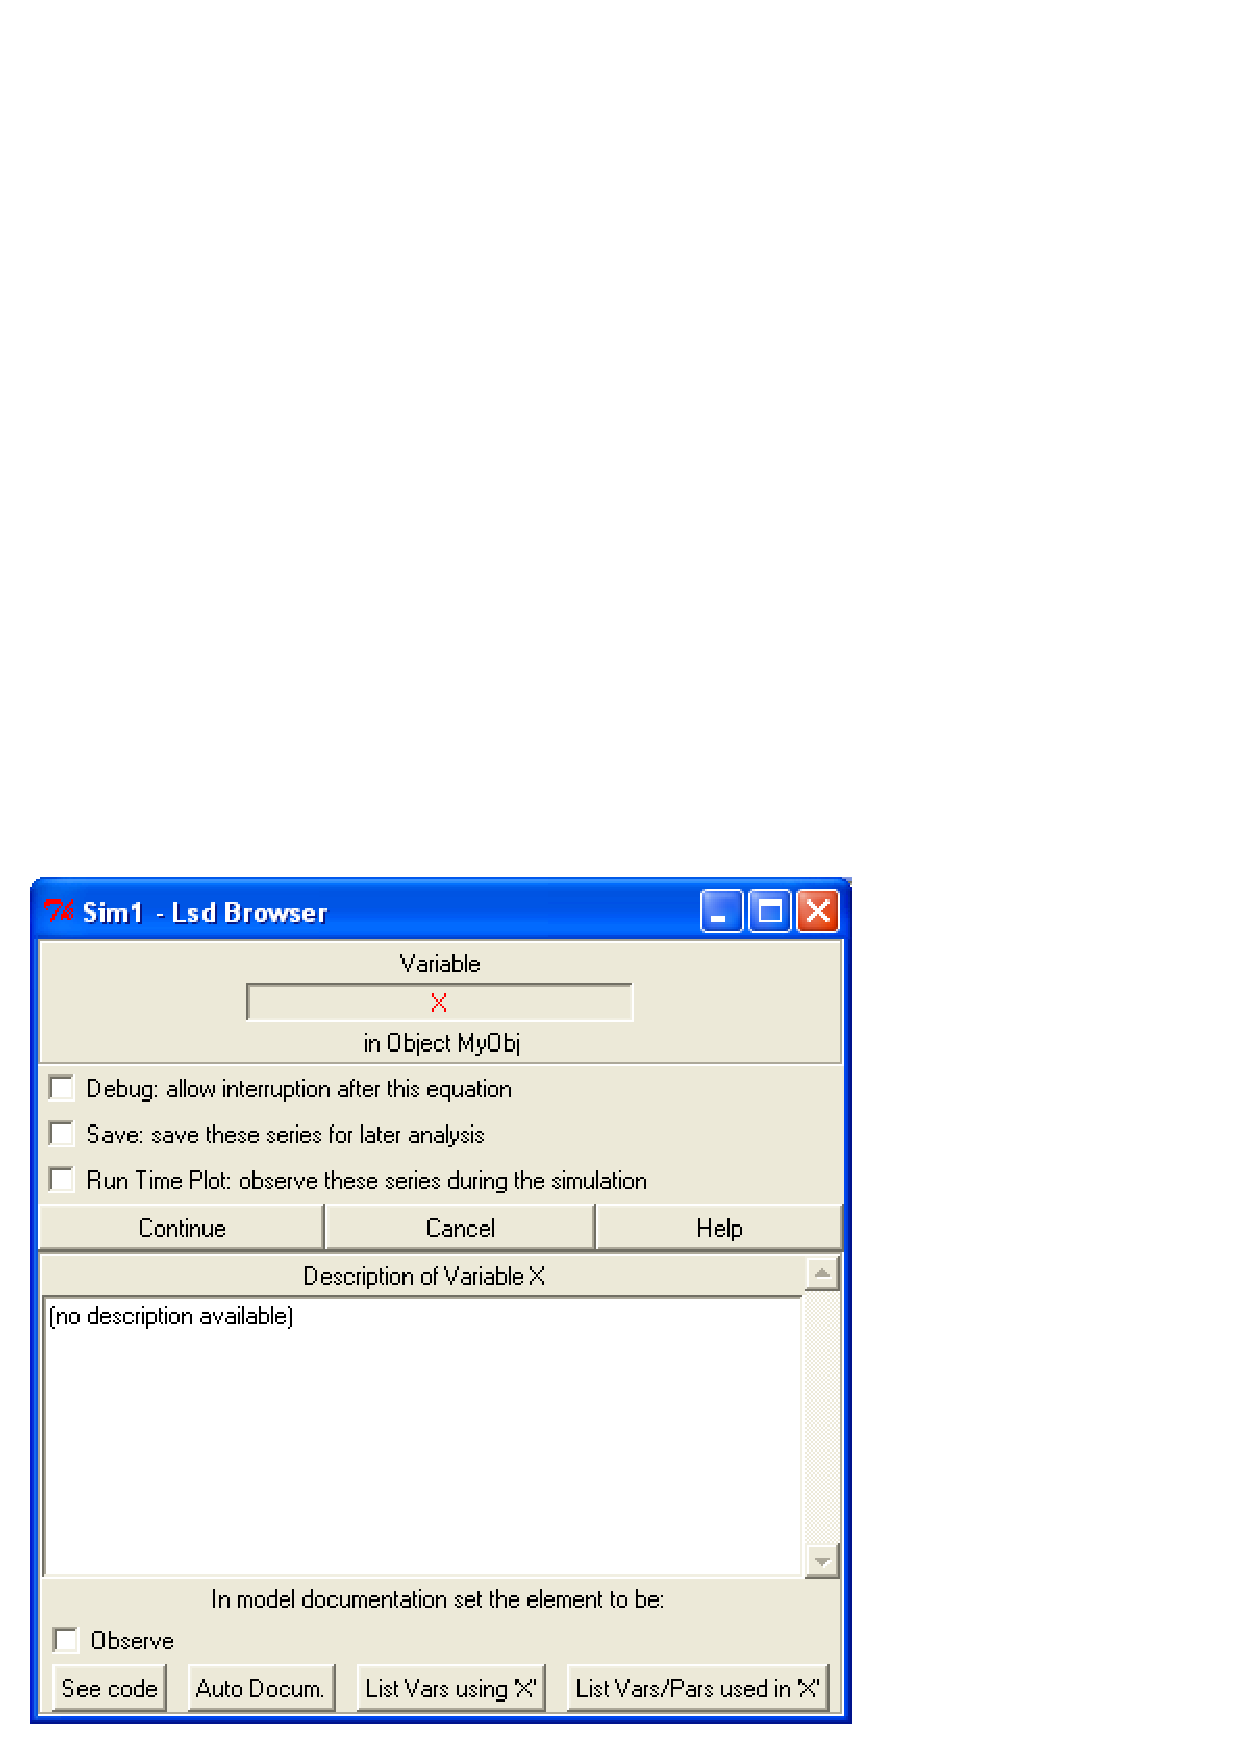
\includegraphics[width=7cm]{variable.pdf}}
  \caption{\LsD variable options}
  \label{fig:variable}
\end{figure}

This window provide access to a set of options concerning a variable. For the time
being we focus on the three checkboxes after the header with the name of the variable:
\menu{Debug}, \menu{Save}\footnote{There are two \footnotesize{\menu{\footnotesize{Save}}} options. The second, saving data in separate files, is rarely used and is ignored in the tutorial for brevity.} and \menu{Run Time Plot}. Check on all the three of them and
click on \menu{Continue} to return to the Browser.

The options we have set we tell \LsD that the values of \LsD must be saved for
post-simulation analysis (\menu{Save}) and that, during a simulation, we want to see the
dynamics of \lsd{X} in a run time plotting window (\menu{Run Time Plot})\footnote{The
\footnotesize{\menu{\footnotesize{Debug}}} option allows to control the internal computation of \lsd{X} during a simulation
run. We will see that later.}. Notice that the two options are independent, so that we
may save the results of a variable without plotting its values at run time, or,
viceversa, observing its values without saving them for post-simulation analysis.

\section{Results of \LsD simulation runs}


Now we can run again a simulation run (menu \menu{Run/Run}). This time, the Log window
does not show the steps completed, because a new window provides the graph reporting the
values of \lsd{X} through the time steps. Being a very short simulation it is likely that before being able to see it the window containing the graph will be covered by the \LsD browser. If necessary, use the icons to highlight the window, or minimize the \LsD browser. 

The Run Time plot window is meant to provide a quick approximation of the simulation results. A more precise presentation of the data produced during a simulation run is produced with the Analysis of Results module, which is devoted to produce a detailed analysis of all the data saved from a simulation run. To access the module from the Browser, choose menu \menu{Data/Analysis of Results}, and the window shown in figure \ref{fig:analysis} will appear. 

\begin{figure}[ht]
  \centering
 \fbox{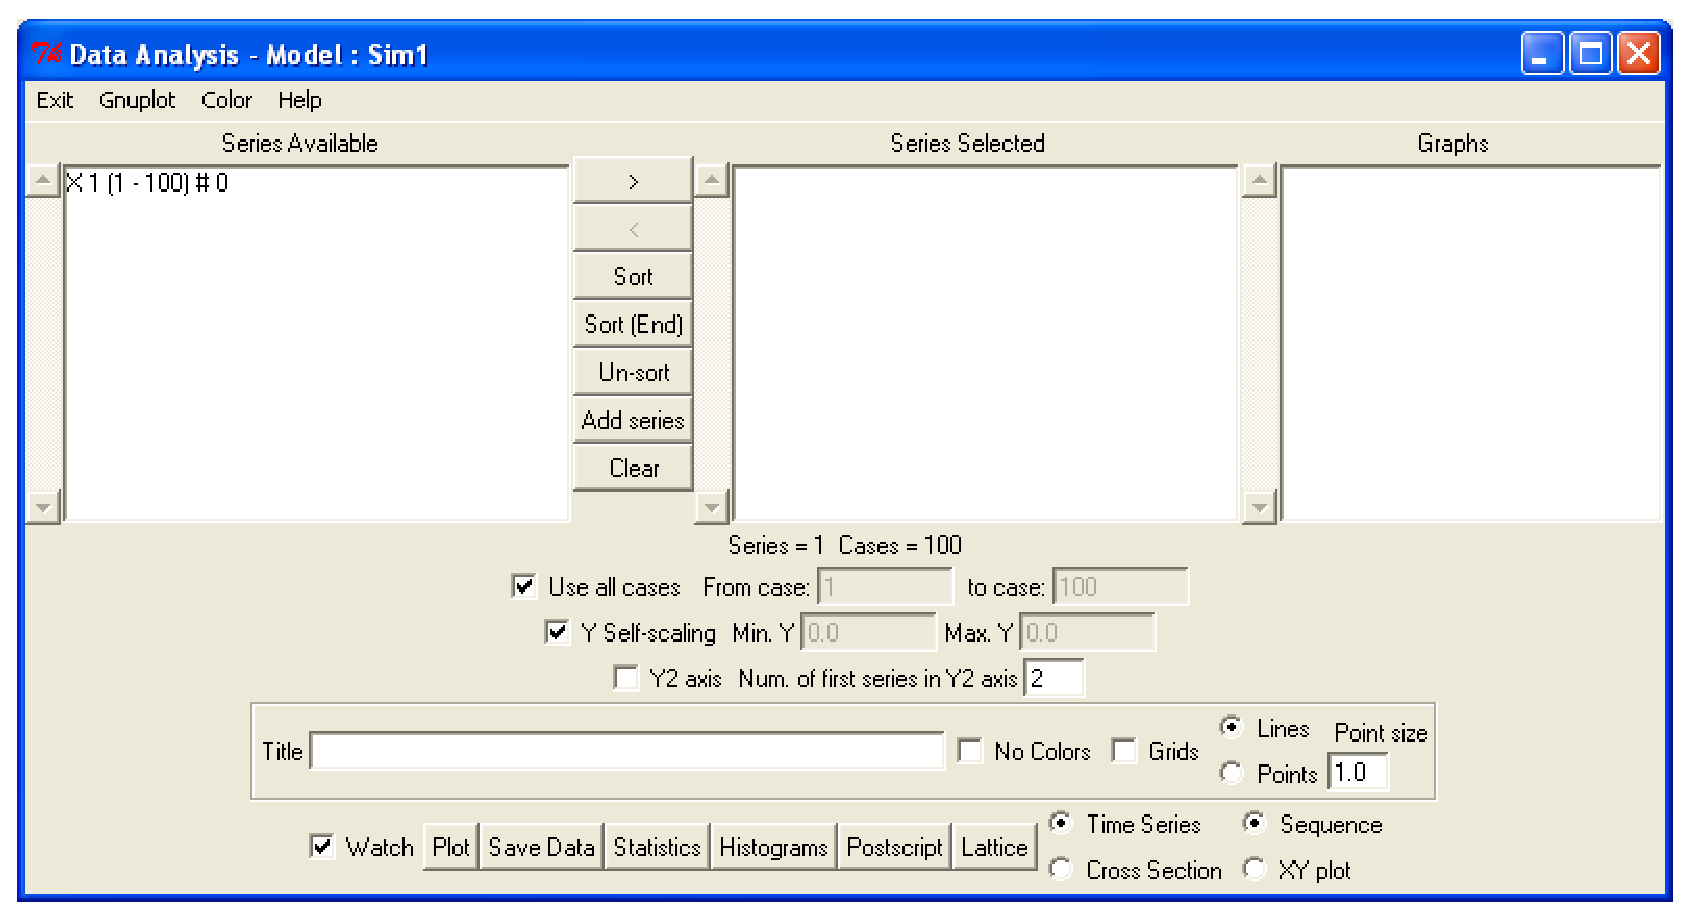
\includegraphics[width=8cm]{analysis}}
  \caption{Analysis of Results window}
  \label{fig:analysis}
\end{figure}

This window allows several ways to present and elaborate results. 

The main body of the window is composed by three lists: \menu{Series Available}, \menu{Series Selected} and
\menu{Graphs}. Selecting the series in the first list you move them in the second list
pressing \menu{$>$} (or double-clicking on the series). The checkboxes in the lower right
part determines how the data must be treated. The default setting are \menu{Time Series}
and \menu{Sequence} asking for the temporal sequence of the data selected. 

The series available (in our case only one) are indicated by their label and other indicators, that we ignore for the moment. Move the only
series in the leftmost list (\lsd{X}) to the the middle list double-clicking on it. Leave the default options
as indicated. Now press the button \menu{Plot}; this will create an equivalent of
the Run Time Plot window, in that the graph shows the time steps on the horizontal axis
and the value of \lsd{X} on the vertical one. This time the graph provides several more
information on the data. For example, hovering the mouse pointer over the window will
give the coordinates of the area under the pointer; when the pointer crosses the line of the graphs the label of the variable appear in the left-bottom corner; double-clicking any part of the graph the main control window comes to the foreground.

Besides plotting graphs the Analysis of Results module provides also some descriptive
statistics. If the Analysis of Result window is hidden below the graph window,
double-click anywhere on the graph. This will bring the Analysis of Result window in the
foreground (this comes handy after you have produced many graphs). Press the
button \menu{Statistics} and observe the \menu{Log} window (search for its icon in the icon bar of the screen). You can see some descriptive statistics concerning the series selected.

The Analysis of Result module in \LsD provides the most commonly used information
concerning the results of the data produced in a simulation. Moreover, it can save the
data in files ready to be imported in other packages for more sophisticated analysis. The
possibilities offered by the Analysis of Results module are fully described in its help
page (\menu{Help/Help} on Analysis of Results). However, many options have no sense for
the moment, since they involve the use of several series and we have only one, so we'd
better exit from this module and explore other aspects of \LsD. Choose menu
\menu{Exit/Exit} to quit the Analysis of Result and return to the Browser. We are going
now to update the equation file, inserting a slightly more interesting equation.
Therefore, quit the \LsD model program, and return to LMM to update the equations for a new \LsD model program.

\section{Extending a \LsD model equations}

The equation we have written is pretty basic. We have defined \lsd{X} as a variable
returning random values in the range [0,1]\footnote{If you don't know how random numbers
are treated by computers, and have never heard the concept of ``pseudo-random number'' or
``seed'', you may want to read the section on this topic in the paragraph
\ref{sec:math_prob} (page \pageref{sec:math_prob}) describing the random functions
available in \LsD.}. Let's review the equation adding two parameters so that the user can
decide the lower and upper limit of the random function. The mathematical formula for a
variable X1 to extend the random variation from [0,1] to arbitrary extremes:

\begin{equation}
 X1 = minimum + (maximum - minimum) * X \label{eq:minmax}
\end{equation}
Equation \ref{eq:minmax} shows that when $X=0$, than $X1=minimum$; if
$X=1$, than $X1=minimum+maximum-minimum=maximum$; for intermediate
values $X1$ varies proportionally to $X$.

Let's implement an equation for \lsd{X1}. If you did not do that yet, close the \LsD model
program (\menu{File/Quit}) since we need to write a new equation in LMM. If LMM, for some
reason, is not showing the equation file, choose menu \menu{Model/Show Equation}.

 In the equation file place the cursor below the line \code{MODELBEGIN},  above the line \code{MODELEND} and not
 inside the code of the equation for X. You are free to decide the order in which the
 equations' code appear in the equation file. \LsD determines, during a simulation, the order of execution of the different variables, so the order in which their code appear in the equation file is irrelevant.

As done before, choose \menu{Edit/Insert \LsD Script} and choose \menu{Equation}. Type the
label \menu{X1} for the new variable and press \menu{Ok}.

In order to compute the values of variables an equation needs almost always to use the
values of other elements in the model, either variables or parameters\footnote{From now on we will consider functions as equivalent to variables, unless otherwise specified.}, and then make
logical or mathematical elaborations on them. To retrieve the value of an element and use it within an equation we need to use a \LsD function called \code{V("label")}, standing for \code{V-}alue of the
element with label ``\lsd{label}''.

Using the \code{V("...")} function, the equation for \lsd{X1} may be written as:


\small
\begin{verbatim}
EQUATION("X1")
/*
  A random value within 'minimum' and 'maximum'
*/

RESULT(  V("minimum") + (V("maximum") - V("minimum") )* V("X"))
\end{verbatim}
\normalsize

Although the equation above is legal and working, writing the elaboration in the \code{RESULT(...)} line is hardly a practical strategy for even minimally elaborated equations. For longer computations a single line will not be sufficient, and anyway the code will be un-readable. It is therefore a good practice to structure the code for the equation with a programming style that minimizes the computations required and improves the clarity of
the code. 

A more efficient style of coding (which becomes a necessity as soon as the equation is even slightly complicated), consists in collecting initially all the values necessary for the computation and storing them into local C++ variables, which are then used to perform the actual computations, possibly with many intermediate computations.

Temporary variables are repositories that live
only within the computation of one single equation, and are re-created any time a variable starts to execute its equation\footnote{This point should be clear. The temporary variables we are going to use cannot be used to transfer values from one equation to another. They are strictly local storage places that needs to be loaded and can be used only within one equation.}. In the equation file modelers have
available the vector of temporary variables named \code{v[0],v[1],v[2],v[3],...}.
Therefore, the equations for \lsd{X1} according to the normal \LsD equations' programming
style is:

\small
\begin{verbatim}
EQUATION("X1")
/*
  A random value within 'minimum' and 'maximum'
*/
v[0]=V("minimum");
v[1]=V("maximum");
v[2]=V("X");
v[3]=v[0]+(v[1]-v[0])* v[2];
RESULT( v[3] )
\end{verbatim}
\normalsize

In the first three lines of the equation we assign the values \lsd{minimum},
\lsd{maximum} and \lsd{X} to \code{v[0]}, \code{v[1]}, and \code{v[2]}, respectively. Then we assign the result of the operation to a fourth local variable, \code{v[3]} and, eventually, its value is used in the result line.



\begin{figure}[ht]
  \centering
 \fbox{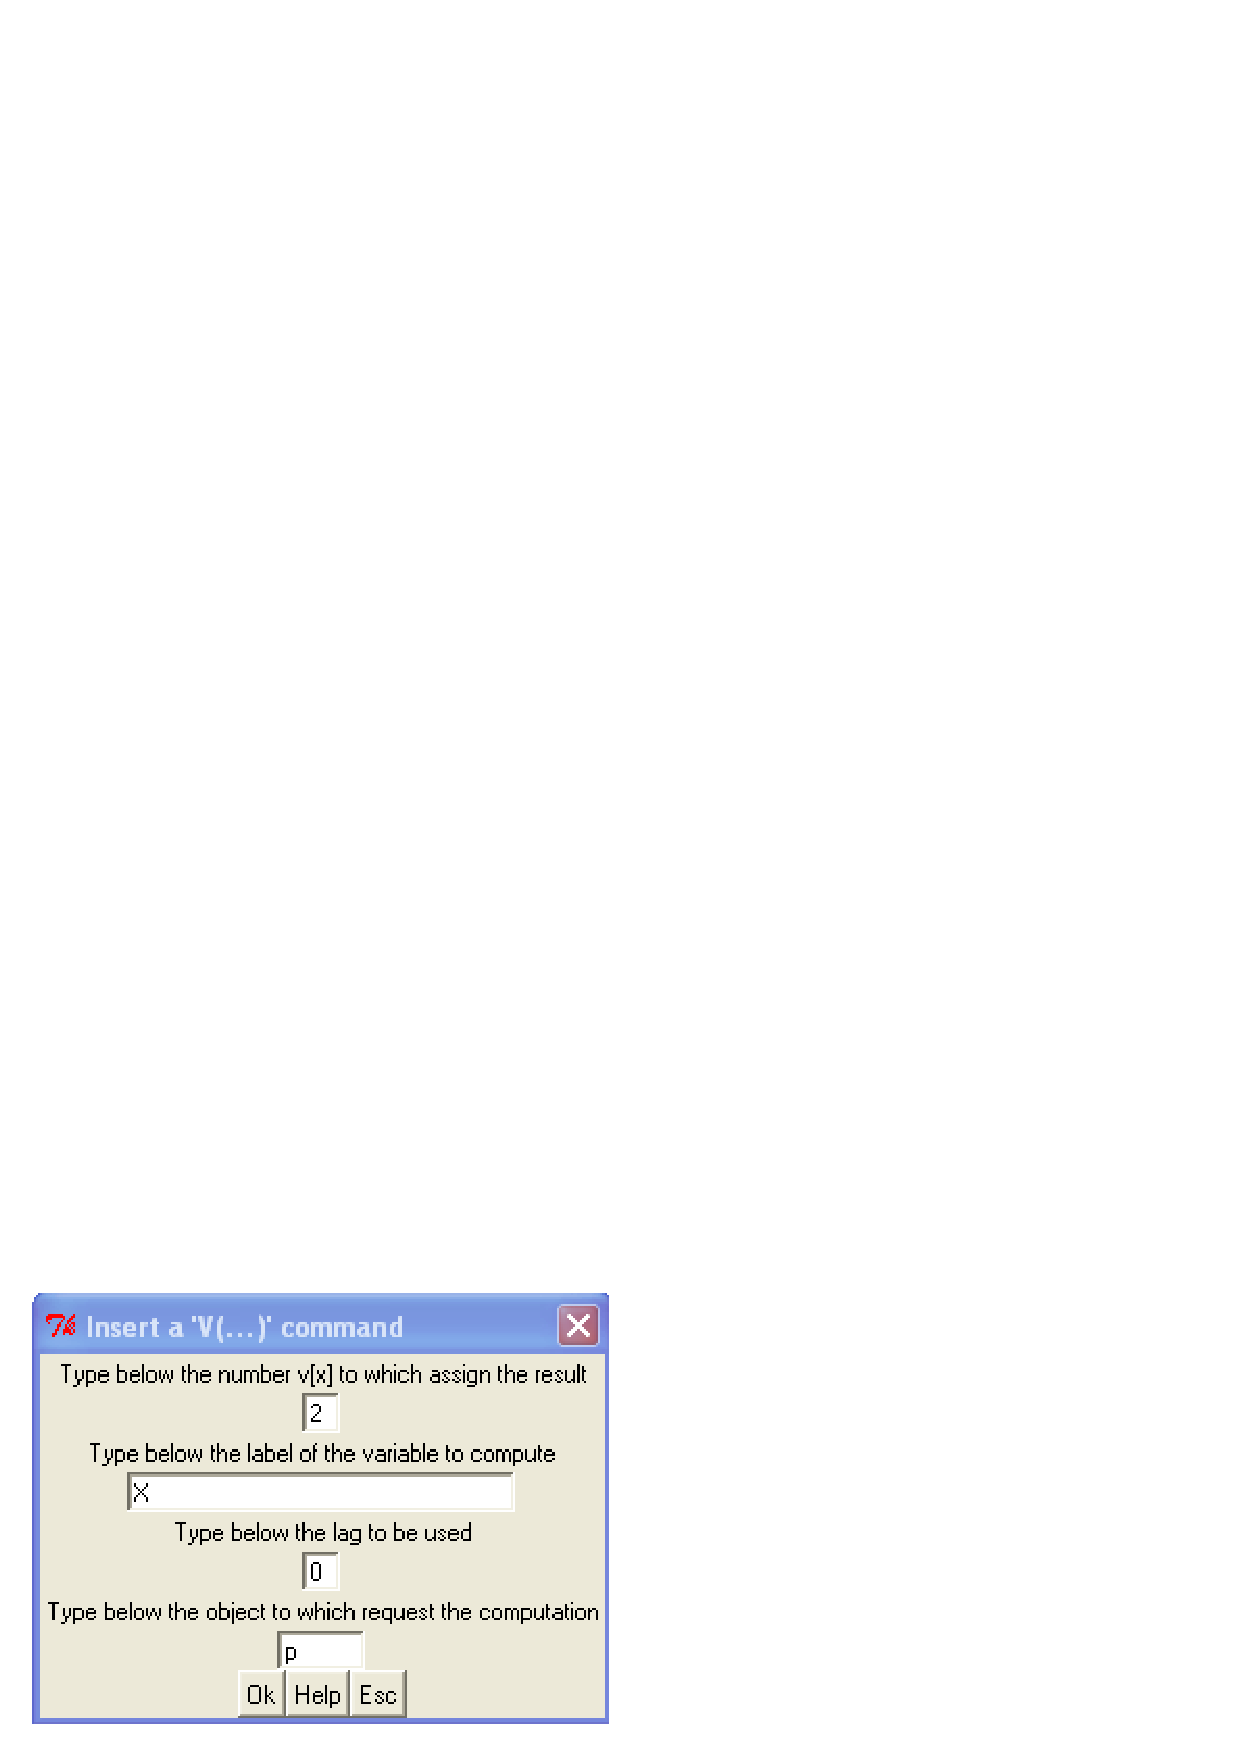
\includegraphics[width=5cm]{scriptv.pdf}}
  \caption{LMM script to insert the equation function \code{V(...)}. }
  \label{fig:scriptv}
\end{figure}

To insert the \code{v[0]=V("minimum");} line and the others we have available a
\LsD script, which avoid trivial, but time-consuming, mistakes and keep tracks of the different local variables used. Trying placing the cursor in the desired location of the editor and choose menu item \menu{Edit/Insert LSD Script} and then choose the option \menu{V("...")}. In
the resulting window choose the desired index for the \code{v[...]} and the type label
for the value to request, that is \lsd{minimum}. Leave the other two options to the default values. Notice that the script moves the focus sequentially through the different fields; you can quickly move the from one field to the next by pressing the \menu{Enter} key without ever using the mouse. 

Repeat the script for all the three elements, inserting a new line after each line is inserted.
Notice that there is no difference in the equation code between using values from parameters or variables.
Actually, a good modeling style consists in implementing earlier versions of the model
with all parameters and only one or few equations. Then, gradually, adding one equation
for a former parameter transformed in an equation. The earlier equations will continue to
work as before, with no change required, even if the internal cycle of computations necessary to update all variables will be different, but this a task performed automatically by the system. 

After having concluded the coding save the file with \menu{File/Save} (or using the
shortcut pressing at the same time the keys \menu{Ctrl+s}).

It is possible that you have typed an error in the code above, for example forgetting a
semicolon at the end of a line, or forgetting one of the nested parentheses. If you try
to run the \LsD model program with such an error the system will issue a warning. A new window will contain the message indicating
approximately where the error has been found, so that you can fix it (see the section
\ref{sec:progr_err} on compilation errors.). 

When a new \LsD model program appears after the compilation we are ready to update the model
configuration adding the new variable and the two parameters.

\section{Initializing \LsD elements}

The new \LsD model program is able to compute a new variable,
\lsd{X1}, but, for this having any effect in a simulation run, we need to add this variable, and the necessary parameters, in the model configuration.

First of all we need to retrieve the model configuration we have defined before: use
\menu{File/Load} and choose the \LsD file (called \code{sim1.lsd} unless you did not change the default name). We need to add three elements to the model: parameters \lsd{minimum} and \lsd{maximums}, and
variable \lsd{X1}. 

Move the Browser to show the \lsd{MyObj} object
and then add the two parameters using \menu{Model/Add a Parameter} and the variable
with \menu{Menu/Add a Variable} (note that the parameters' labels in the Variable list
have appended the symbol \menu{(P)}).

Beware that the spelling of variables and parameters in the \LsD model program must
perfectly match their spelling in the equation file, and that lower/upper capital letters
matters. If a variable or parameter with the wrong spelling is inserted it is possible to
edit its label. To do this double-click on the label of the element to edit so to open
the option window for that element (see fig. \ref{fig:variable} at page \pageref{fig:variable}). In this window you can double-click on the red label of the element in the upper part of the window and a new window will appear, as shown in figure \ref{fig:edit_var}. This window allows to change the label for the element (assign an empty label to remove it altogether), change its position in the object structure, or change its nature (e.g. from parameter to variable).

\begin{figure}[ht]
  \centering
 \fbox{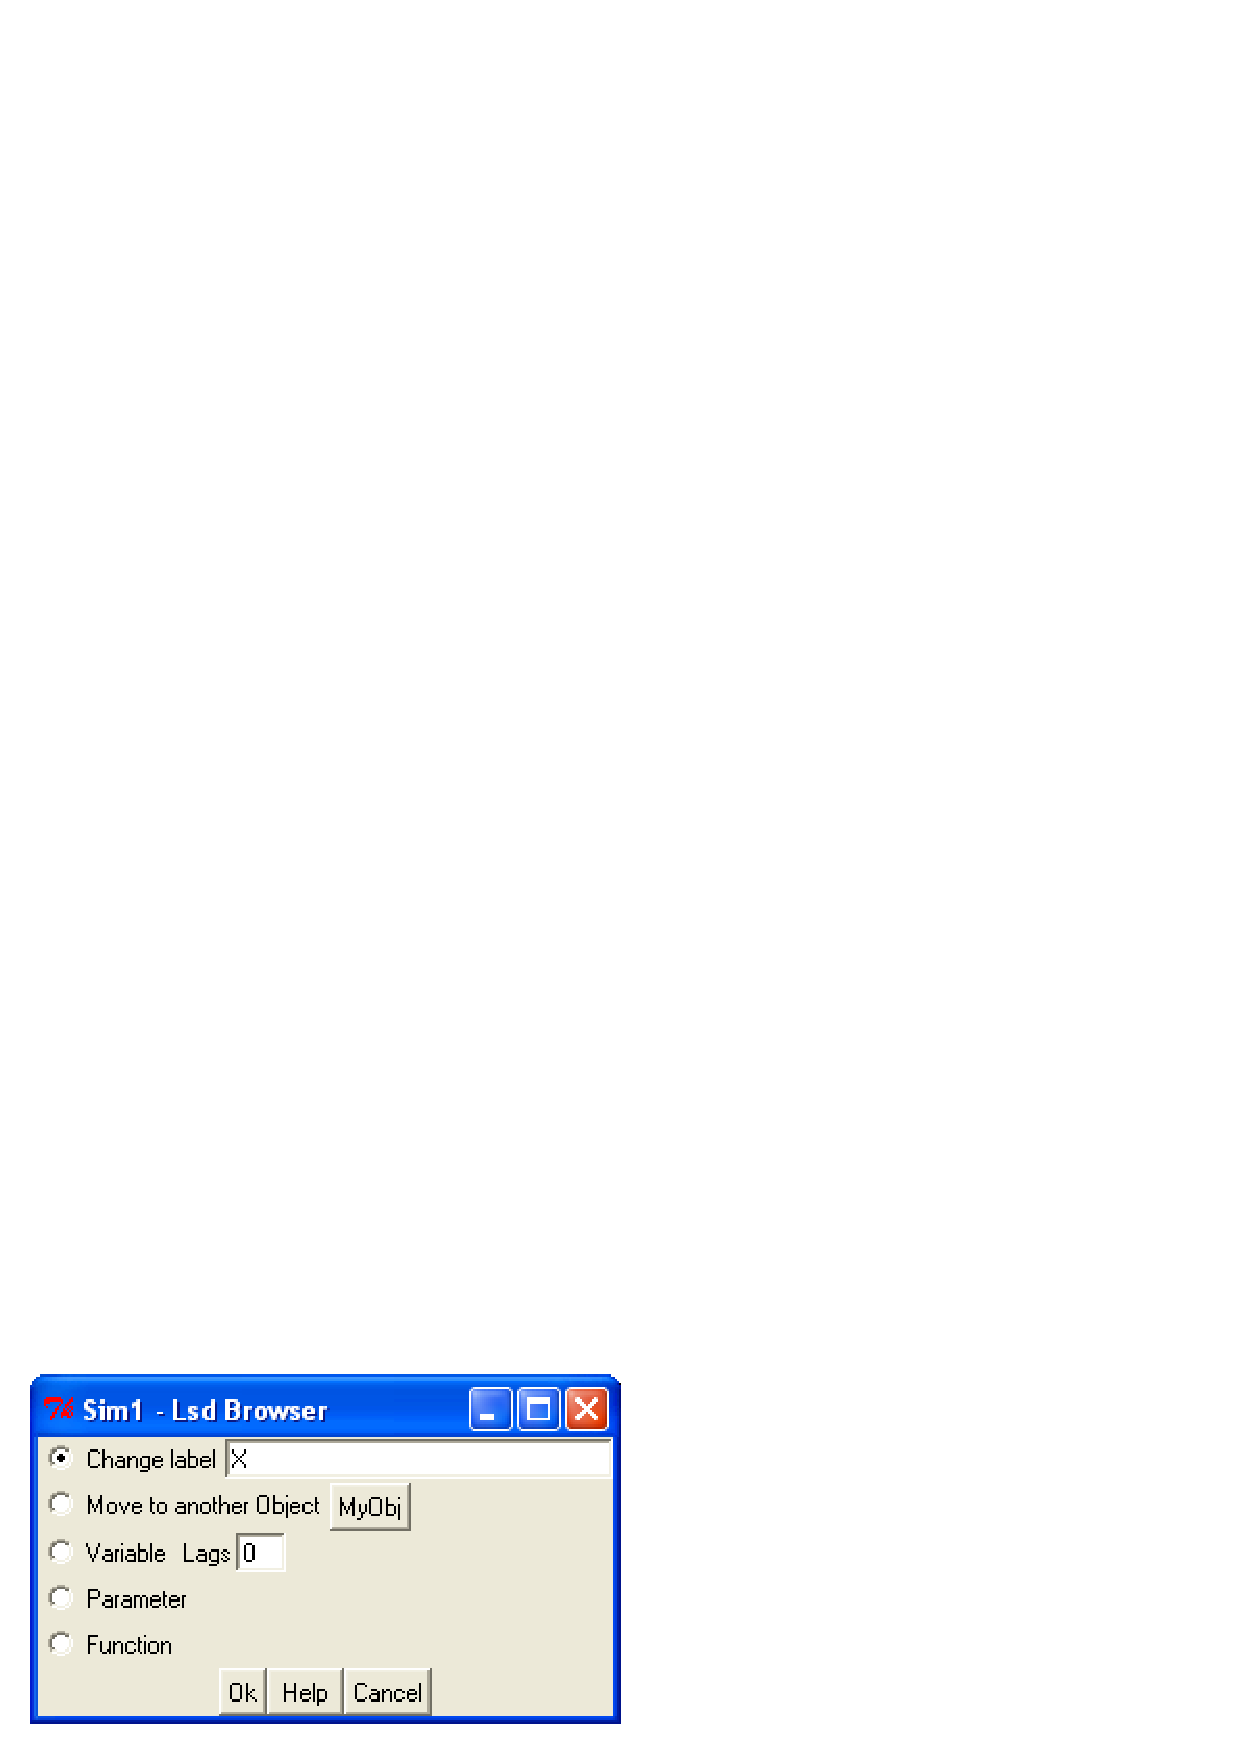
\includegraphics[width=5cm]{edit_var.pdf}}
  \caption{Options to modify an element. It is possible to turn the element into a parameter, variable or function; change the label of the variable; delete it altogether (assigning as new label an empty string); move it to a new object.}
  \label{fig:edit_var}
\end{figure}


After having inserted the new elements we are still not able to run a simulation. In
fact, the two newly inserted parameters need to be initialized, and an attempt to run a
simulation would cause an error message to be issued and the simulation run aborted (try it, and then re-load the configuration to return to the current configuration). 

To assign a value to the parameters in an object\footnote{\LsD permits to assign initial
values only to the elements of one type of object per time.} you need to place the
Browser to show the object concerned and then choose menu item \menu{Data/Init. Values}.
The Browser window is then transformed in a table showing one line for each element to
initialize, as shown in fig. \ref{fig:init}.
\begin{figure}[ht]
  \centering
 \fbox{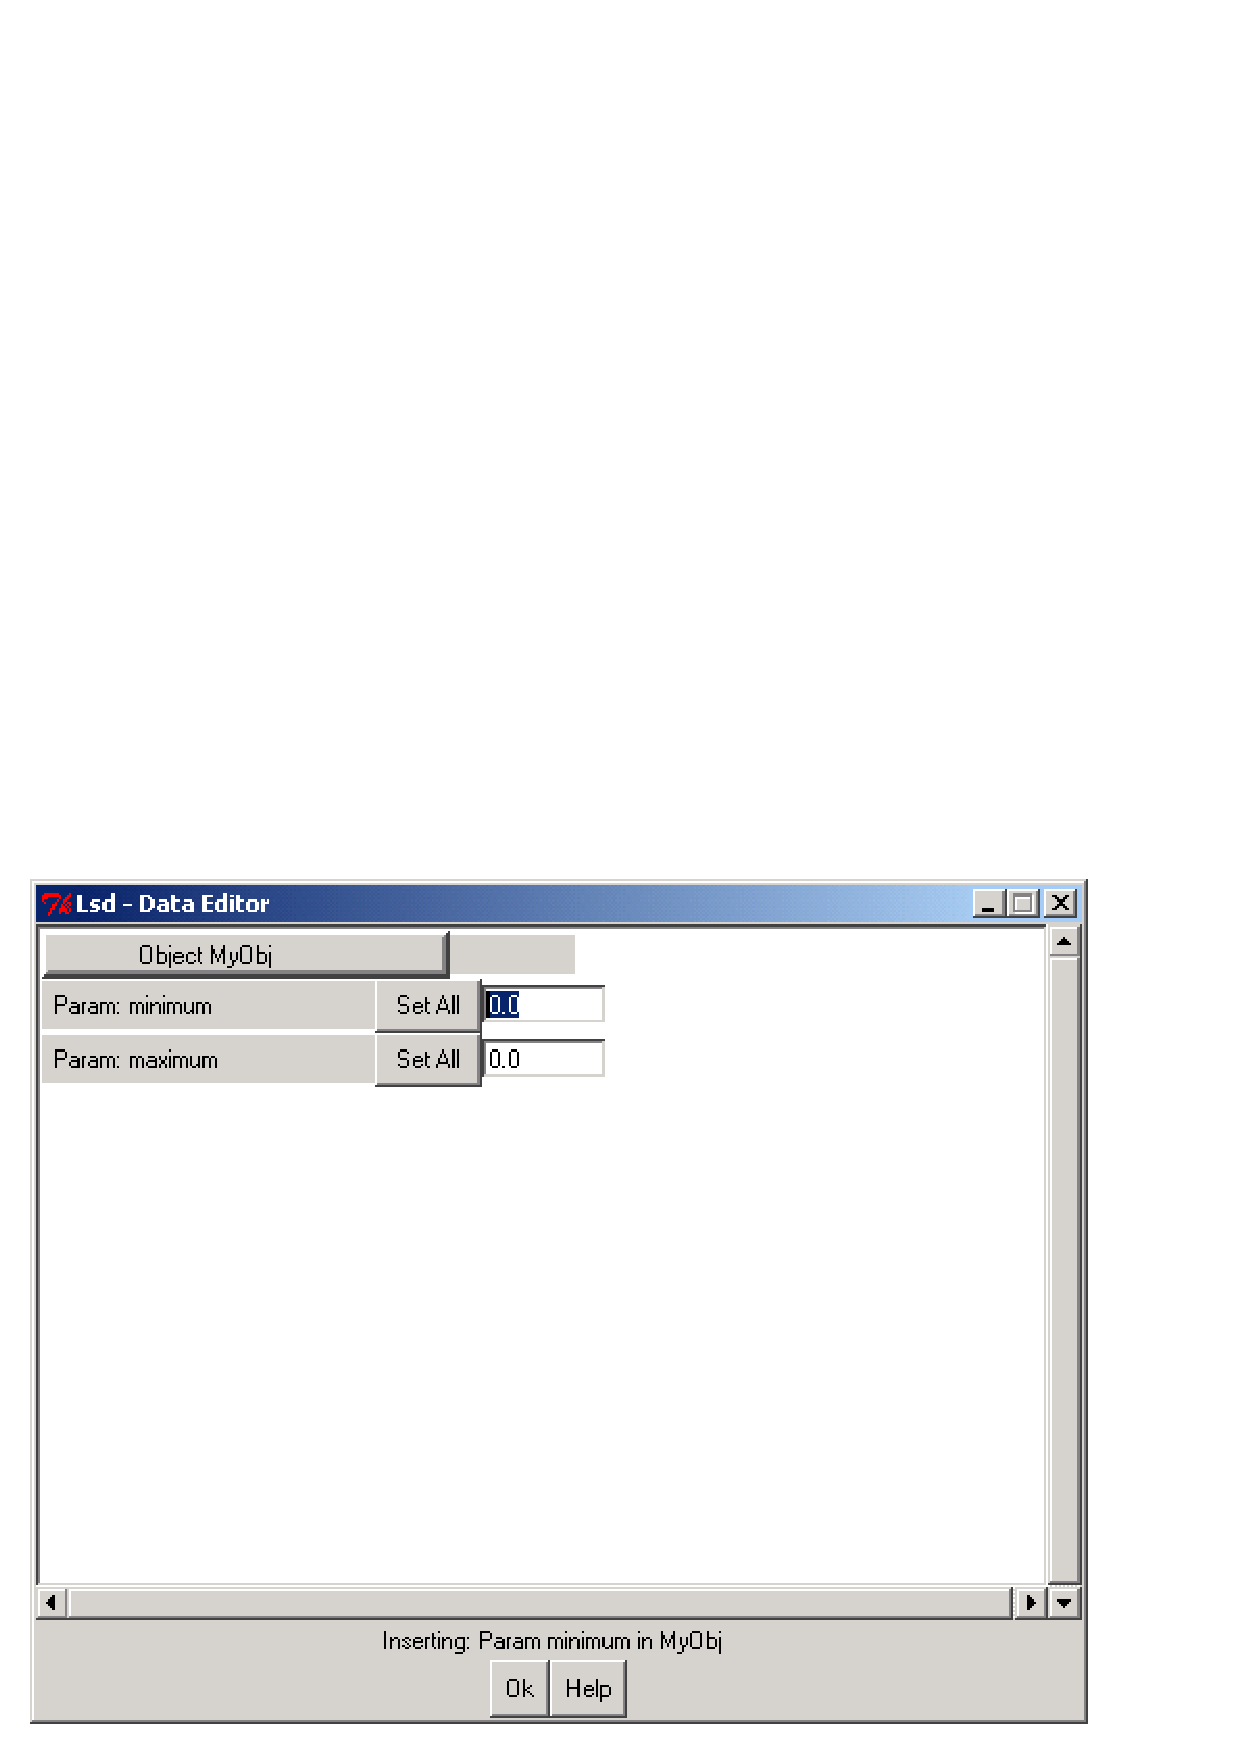
\includegraphics[width=10cm]{init.pdf}}
  \caption{Initial values for \lsd{MyObj}}
  \label{fig:init}
\end{figure}

By default \LsD assigns a value of 0 to each element. You can type into the cells the
elements desired, say -100 for minimum and 100 for maximum. Notice that the initial value
window does not show the elements that do not need to be initialised, like \lsd{X} and
\lsd{X1}. At the end of the initialization press \menu{Ok} to return to the Browser.

Now we could run a simulation, although we may want to save the results of \lsd{X1}.
Double-click on this variable in the Browser and set on the option \menu{Save} and the option
\menu{Debug}. Now we can run the simulation. The Run Time Plot window will report only
the series of \lsd{X}, as before, because we did not set the option \menu{Run Time Plot}
for variable \lsd{X1}. However, the values of \lsd{X1} have been saved and we can observe
them in the Analysis of Results window (menu \menu{Data/Analysis of Results}). This time
we have two lines in the list of the series available, one for \lsd{X} and one for
\lsd{X1}. Observing their graph we see that they have the same dynamics, but, as expected, their range differ for the scale.


As a matter of exercise, we can produce a scatter-plot graph, where two values of the two variable at the same time step correspond to a point. In the Analysis of Results window check the box \menu{Time Series} and the box for \menu{XY plot}. Choose also the option \menu{Point} to generate a graph with dots and without a line interporlating the points. Insert in the \menu{Series Selected} list firstly the variable \lsd{X} and then \lsd{X1}. After clicking on the button \menu{Plot} a new window asks whether you want to generate a high-quality or low-quality graph; press \menu{No} and a new graph will appear\footnote{Scatter plot graphs are generated using an external package, Gnuplot. \LsD allows either to incorportate the graph as image within a \LsD graphical window, or to use a Gnuplot window. In the former case you loose some of the quality, but you can manage the window as any other \LsD window. Gnuplot windows are instead managed by its own commands. Test both options, to appreciate the difference.}
This graph shows the values of \lsd{X} on the horizontal axis and the corresponding value
(i.e. at the same time step) of \lsd{X1} on the vertical one. 


After having produced the graph, exit from the analysis of results module and return to the
Browser. Since the \LsD model program contains the data from the latest time step, reload
the configuration. You can use the menu \menu{File/Re-load}, or the short-cut
\menu{Ctrl+w}.


\section{Setting the number of objects}

We have worked with one single copy of the \lsd{MyObj} object. The main advantage of objects is that they can be multiplied in as many copies as desired, generating automatically all the copies of their content, including, if present, sets of copies of contained objects.

Open menu item \menu{Data/Set Number of Objects/All types of Objects}. The Browser
window will become as in fig. \ref{fig:numobject}.

\begin{figure}[ht]
  \centering
 \fbox{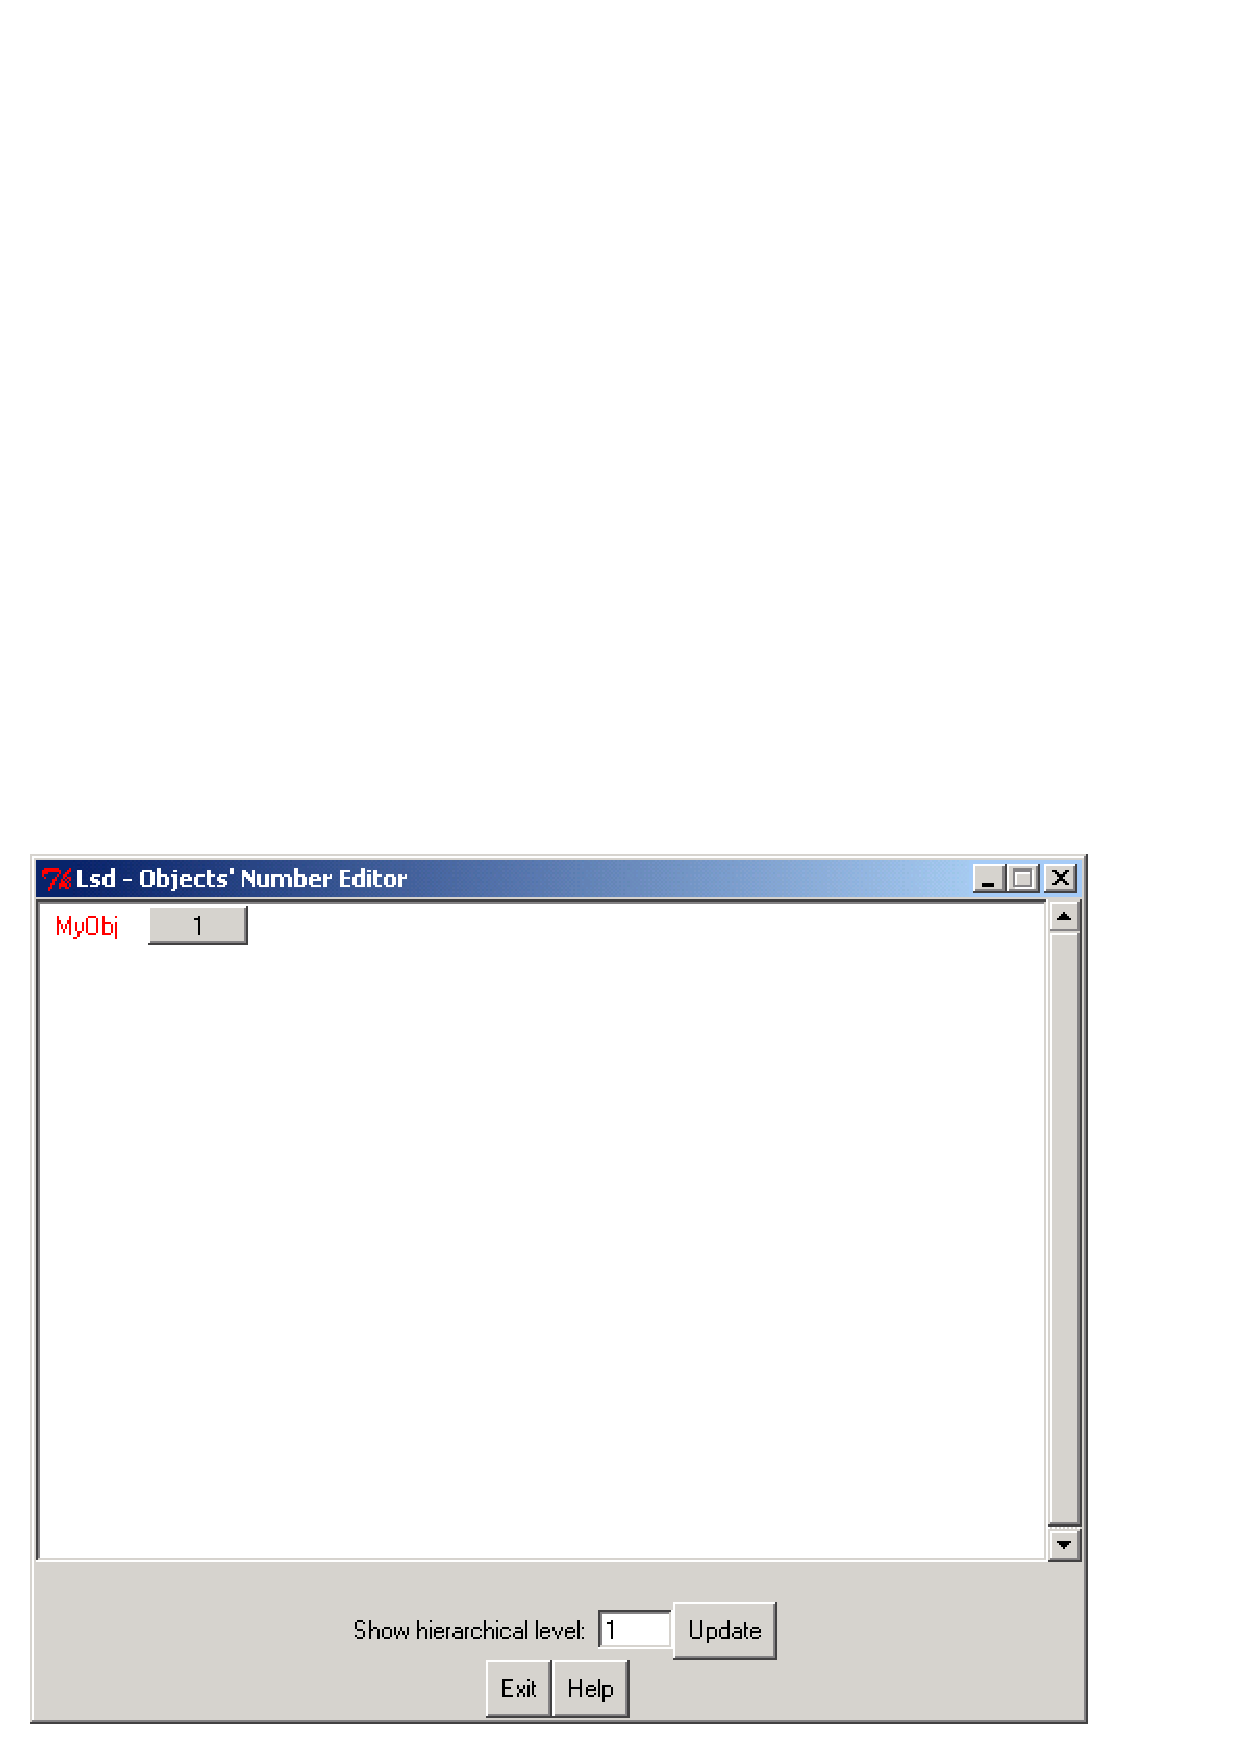
\includegraphics[width=10cm]{numobject.pdf}}
  \caption{Setting the number of Objects}
  \label{fig:numobject}
\end{figure}

This table shows only one line, since there is only one type of object. Click on
the number on the side of label for \lsd{MyObj} and insert the number of copies of this
object you want in your model. For example, type 10. Pressing \menu{Ok} you return to the
Browser. As you see, nothing is changed, since the Browser shows only the structure of
the model and not the number of copies. However, the graphical representation of the
model now indicates that there are 10 copies of \lsd{MyObj}'s in the model.

The new copies have been created as identical copies of the only one previously existing,
and therefore also the initial values for \lsd{minimum} and \lsd{maximum} are identical
in all the copies, and the same settings for the elements (e.g. variables to save and/or
to plot at run time) are applied. When adding new copies one generally is interested in changing the initial values of their elements.

\section{Initializing multiple elements}
Open the menu \menu{Data/Init. Values} to control for
the parameters' values\footnote{If the initialization window is empty check that the browser is showing the right object. Initialization can be made only for one type of object.}. Given the number of copies of \lsd{MyObj} now there are 10 copies for each type of parameters. Though it is possible to insert manually new values in each cell, the process is impractical as soon as there are a few tens of elements to initialize. To avoid this tedious work \LsD offers the possibility to use one of several automatic functions to generate values for each line, that is, for each type of element to initialize.

The button \menu{Set All} on the right of a label allows to set all the initial value for a
parameter according to one of the available rules. For example, set the \lsd{minimum}
values to increasing values starting from -100 and changing of 10 for each object. For
doing this with \menu{Set All}, click on the button on the right of the label for
\lsd{minimum}. Check on the option \menu{Increasing}. In the box labeled ``Numerical data ...'' there are two entry cells: type in the top cell, marked as \menu{Start}, -100 and, in the second entry marked \menu{Step} enter 10. Press \menu{Ok} to confirm and exit. Now \lsd{minimum} is set to -100 for the parameter \lsd{minimum} in the first object, to -90 for the second, etc. Set also \lsd{maximum} as starting from 100 and changing of -10 at each step. This will make the ten copies of \lsd{X1} oscillating on decreasing ranges. 

\section{Plotting multiple series}
Running a simulation with the 10 copies will make no difference but that the series shown
in the Run Time Plot have now become 10, identified with different colors and assigned a
different number. Run the Analysis of Results after the simulation. You will see that there are now 
10 series for each variable saved, each identified with a different
number placed after the name of the variable. You can choose as many variables you want to plot, by selecting them and then clicking on the \lsd{$>$} button, or double-clicking on each of them. The selection rule respect the usual criteria:
\begin{itemize}
	\item Click and drag: all the variables touched will be selected;
	\item Click on one series, keep key ``Shift'' pressed and select another series. All intermediate series will be selected too.
	\item Click on several series keeping key ``Control'' pressed. Every series will be added to the selection.
\end{itemize}

As you can see, the series in the \menu{Series Available} are listed according to the sequence of objects containing them, so that variables \lsd{X} and \lsd{X1} are listed alternating. Since frequently we need to select all the copies of one type of variable, the standard selection rules are rather cumbersome. There are other two ways to perform this type of selection quickly and effectively.

Firstly, it is possible to click on the button \menu{Sort}. This will rank the series according to their increasing alphabetical order, therefore placing together all variables with the same label. Secondly, we can use a rather sophisticated selection function, which is extremely helpful when dealing with many thousands of variables.

Move the pointer of the mouse over one of the variables you want to select, and click with the right button of the mouse. A new window will pop up, as the one shown in figure \ref{fig:selection}.

\begin{figure}[ht]
  \centering
 \fbox{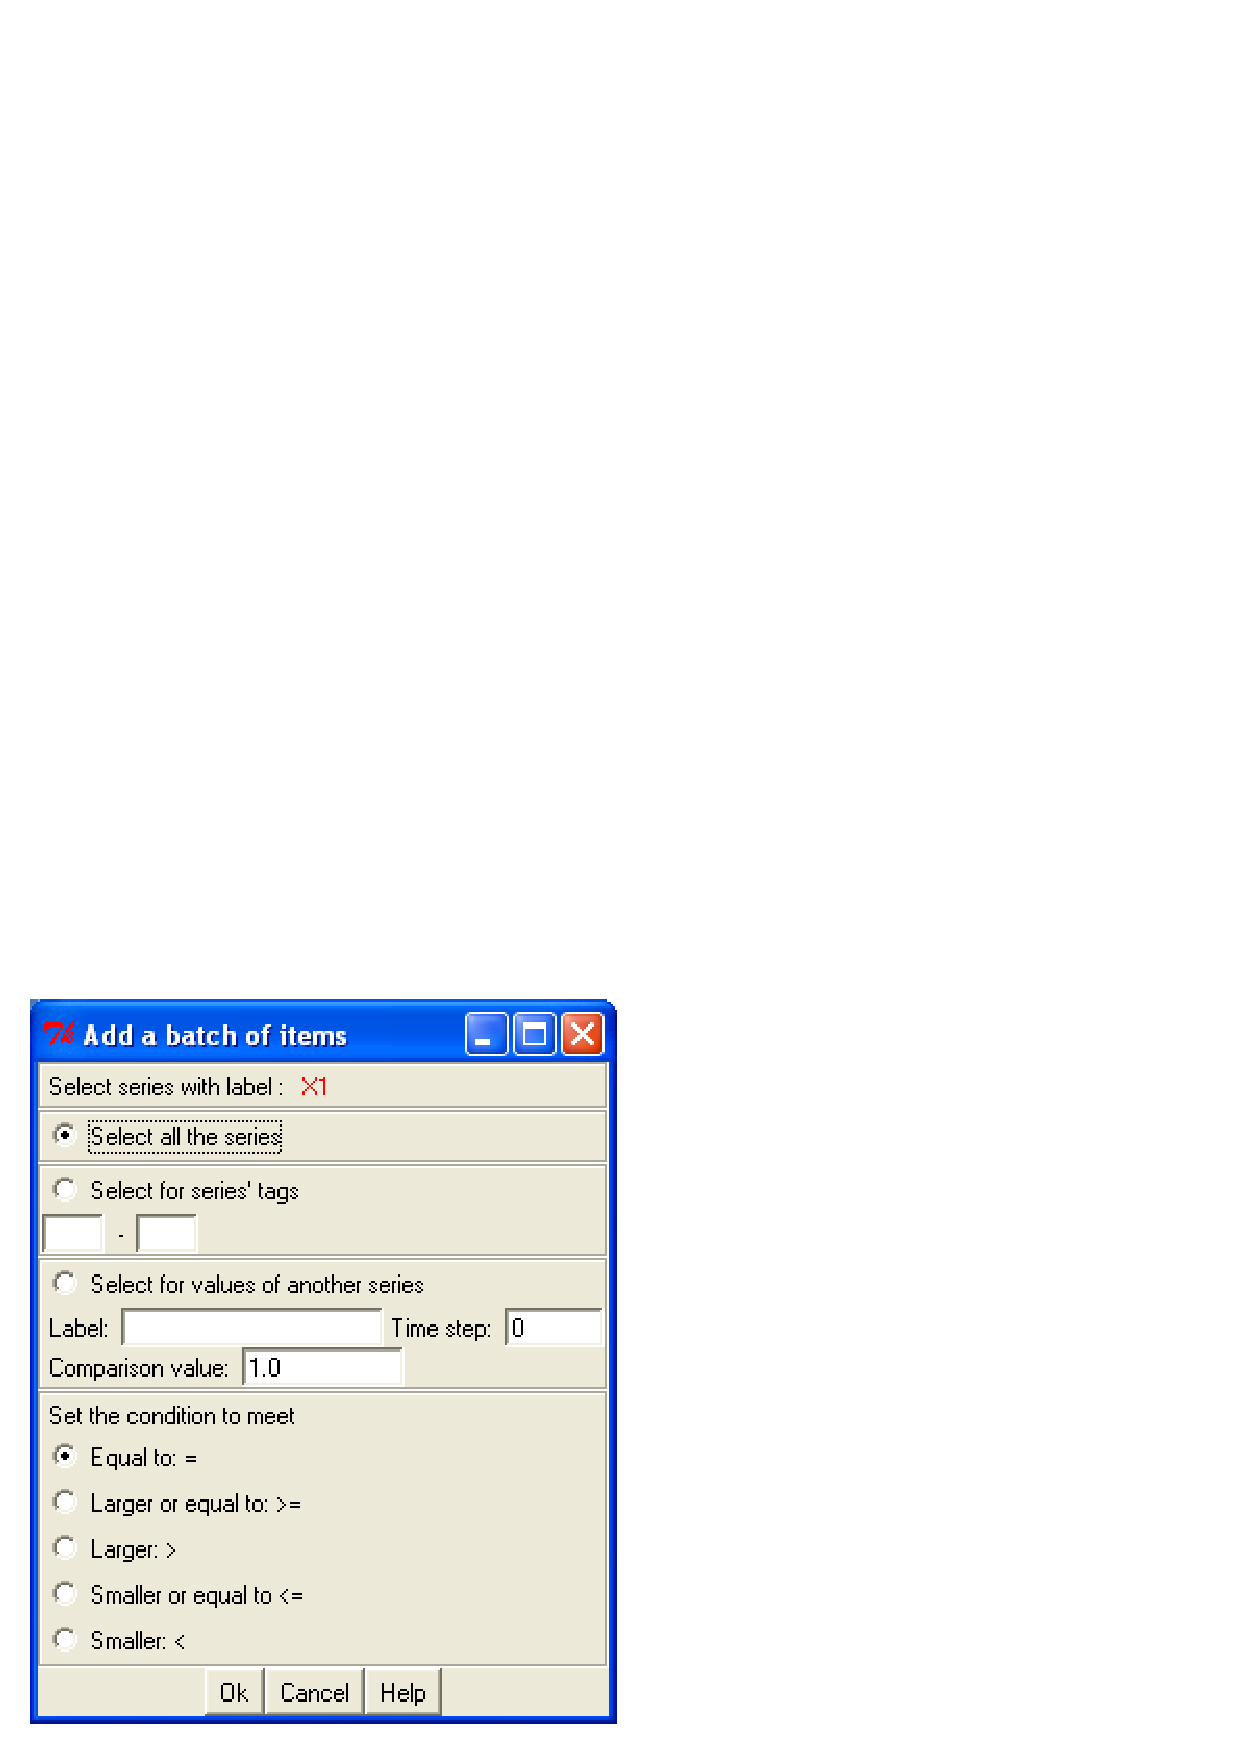
\includegraphics[width=5cm]{selection.pdf}}
  \caption{Selecting function in Analysis of Results window.}
  \label{fig:selection}
\end{figure}

This windows allow to select and move into the \menu{Series Selected} box all the series with a given label, respecting certain conditions. Let's ignore the options available (or see the \menu{Help} button for details), and leave selected the top-most option, \menu{Select all series}. Press \menu{Ok} and all the series with the label will be moved into the central box. Pressing the button \menu{Clear} will empty the \menu{Series Selected} list box.

\section{Statistics}
We can now press the button \menu{Plot} and generate a graph including all the series selected. The initialization we gave to the parameters let us expecting that the oscillations of the variables in the earlier objects should larger than those in the later ones. However, the graph shows independent random series, and therefore it is difficult to individuate whether the expected property does actually occur.

The easiest way to assess the properties of the series is to check the variance of the different series. Click on the button \menu{Statistics}, and search for the \menu{Log} window. The window will contain one line of statistics for each series selected, indicating: label and object's indicator of the series (along with the number of data considered); average value; variance; minimum; maximum; and standard deviation.

As expected the average values are all around zero, the expected values of all the random variables, while the variances decrease for the increment of the objects' indicators.


\section{Comments on equations' code}
The results we have obtained are quite obvious: each of the 10 copies of the object
computed the equations producing independent results. \LsD automatically induced that the copy of the variable \lsd{X1} placed in the $i^{th}$ object had to use the parameters contained within the same copy of the object, dispensing the modeller to insert redundant information as an index $i$.

This feature is extremely useful when the object structure of a model becomes even slightly elaborated, with many layers of objects. When an equation is computed the same code must be exploited by all the variables with the same label, included in different copies of the same type of objects. How can we be sure that the equation makes use of the ``correct'' elements, when the model contains many copies of each of them?

\LsD ``knows'' the copy of the object containing the variable under computation. By default any element appearing in the code of the equation is searched within the same object containing the computing variable. If the required elements are not there, then \LsD moves on to search in ``nearby'' objects, continuing until the whole model is scanned. This feature has many useful consequences. For example, as we have seen, the modeller needs not to specify within an equation where the elements required are stored, and the same code can be used in several object structures. Obviously, the modeller can, if necessary, force \LsD to make use of a specific element, by indicating which object should be searched for an element, though this is rarely needed.


In our case, the \lsd{X1} variables are placed within an object together
with the parameters \lsd{minimum} and \lsd{maximum} necessary to compute them, and
therefore the \code{V("...")} returns those copies. For example, the copy of \lsd{X1} in
the 3$^{rd}$ object  will compute its equation making use of the copies of \lsd{minimum},
\lsd{maximum} and \lsd{X} contained in the same 3$^rd$ object. As we will see,
programmers have a wide variety of options to write code that makes use of values from users' specified
objects. However, in the vast majority of cases you will not need to use these
options, and can rely on the \LsD system to retrieve the correct values for you.


Exit from Analysis of Results and re-load the configuration with \menu{Control+w}, so that we can see
another aspect of configuring a simulation run.

\section{Simulation settings}
The simulation runs we have launched up to now have all done 100 steps, since this is a
default value assigned to a new model and we did not modify. Of course, users can edit
this and other options for controlling the simulations that do not concern directly the
computation of the model. These options are set using the menu item \menu{Run/Sim.
Settings} which shows a window as in fig. \ref{fig:simset}.

\begin{figure}[ht]
  \centering
 \fbox{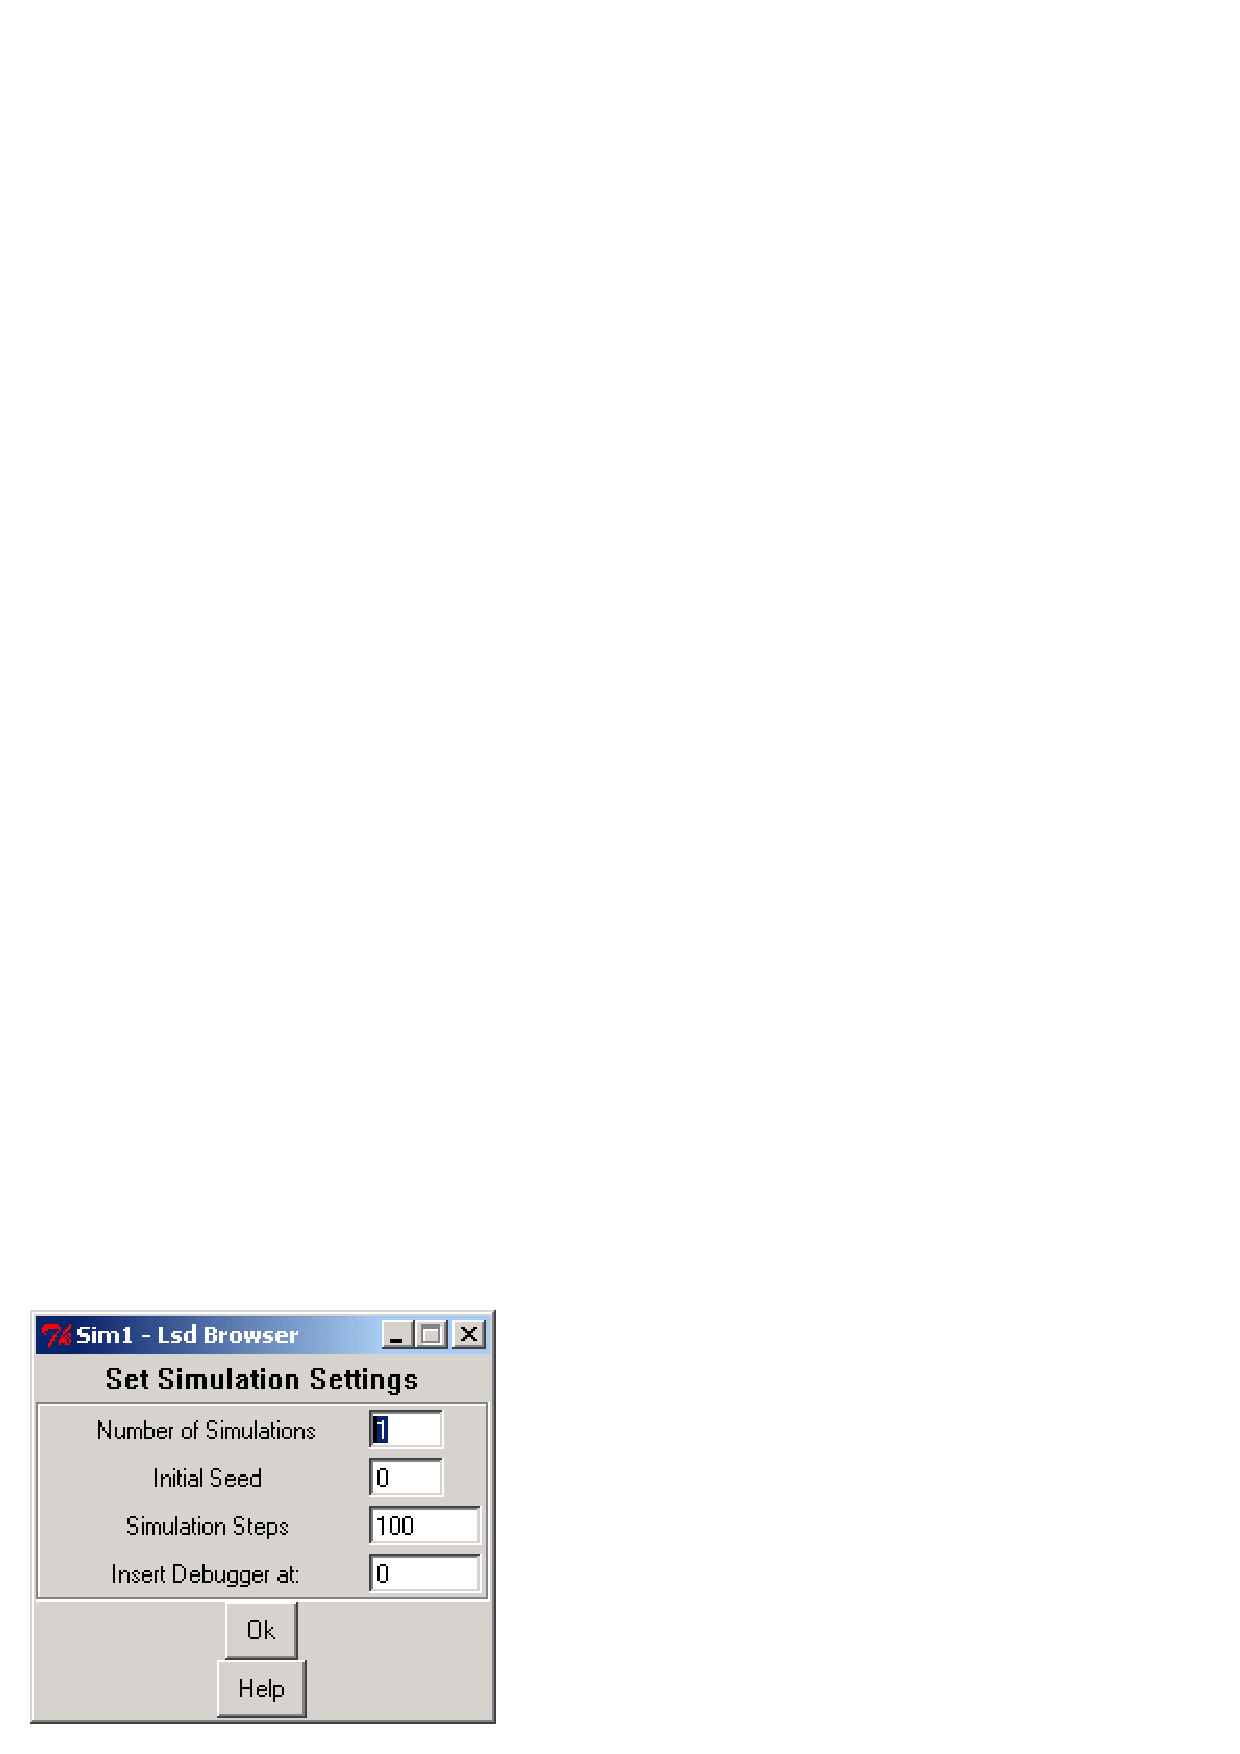
\includegraphics[width=5cm]{simset.pdf}}
  \caption{Setting simulation options: number of simulation runs, time steps per run, pseudo-random values, and debugging options.}
  \label{fig:simset}
\end{figure}

The options control the following behaviour of the simulation runs:

\begin{itemize}
  \item \menu{Number of Simulations}: by default users run one single simulation per
  time, control the results and then change either initial values or the equations before
  testing another (single) simulation run. The results are stored in memory only, unless the user saves them explicitly after the simulation run.
  However, in certain cases one may be interested in
  knowing how the model behaves repeating several times the simulation using different
  random values, to test the robustness of some result. In these cases users can set
  the number of simulation runs to be higher than 1. The results of each simulation run
  (i.e. the data produced during the simulation by the variables marked to be saved) are
  stored into files (with extension \code{.res}) at the end of each simulation run. Moreover, the system generates
  a summary file (extension \code{.tot})
  containing the very last value for each variable so to compare the values
  of saved variables from different simulations. Analysis of results can load any of
  these files and analyse the results there contained.
  Notice that if any variable is supposed to create Run Time Plots during a simulation, every simulation will produce a
  new Run Time Plot. If you set ask for 100 simulations, this will create 100 windows.
  The menu item \menu{Run/Remove Run Time Plots} will remove all the windows at once.
  \item \menu{Initial Seed}: computers are not able to produce random events.
  However, there are numerous mathematical tricks that provide sequences of values that
  have the same properties as random values. Setting the same ``seed'' for repetitions of the same simulation
  implies the use of exactly identical ``random'' events (which, in fact, are 
  called ``pseudo-random'' events). Instead, setting different seeds produces different
  random events. If there are more than one simulation runs to be executed, the system
  automatically provides increasing seed values at the starting of each simulation
  run, and the same seed value is used to name the file where the results are stored, so
  to be able, if necessary, to reproduce one specific run with the same (pseudo-)random
  events.
  \item \menu{Simulation steps}: the number of steps to be executed for each simulation
  run. 
  \item \menu{Insert debugger at: }: most of the time spent by programmers on whatever
  software project does not concern writing code, but the investigation of anomalous
  behaviour of the program, like unexpected crashes or absurd values. Simulation
  modelling is not an exception to this rule, so \LsD provides a ``debugger'', that is a
  function that supervises the running of a simulation and, if necessary, interrupts it
  giving the modeller access to each and every value of the model in order to control
  what is actually going on in the model at that time. With this option users determine
  at which time step the debugger must be activated. If this value is 1, then the debugger
  is active from the very time step. If it is 0 or a negative value, the debugger is
  never activated. If it is, say, 56, then the debugger is activated at the $56^{th}$ time
  step. When the debugger is active the simulation is interrupted as soon as one of the
  variables marked to be debugged (see variables' options, fig. \ref{fig:variable} at
  pag. \pageref{fig:variable}) completes its equation\footnote{Notice that \LsD users can also use standard
  C++ debuggers, like GDB (included in the Windows distribution) which instead give access to a simulation run not every
  equation completed, but every single line of code completed. However, the use of these debugger is quite complicated, and does not allow to access model data. Instead, using the \LsD debugger is simpler and gives full access to any data of the model, including using the Analysis of Results module on the data produced up to the time of interruption.}.

\end{itemize}


All the settings above, but the last one concerning when to activate the debugger, are
stored in the file together with the model configuration.



\section{Using lagged variables}
One of the main reasons for using simulation models is that understanding the result of
even simple temporal dynamics is very complicated. The equation we have implemented until
now are not really dynamical, since they compute values as elaboration of present-time
values, that is, at the same time step. We have a real dynamics when we make elaborations
over values from the past.

The possibly simplest dynamical function is the so called \emph{random walk}. The equation for
random walk is (note that we now use the temporal index t):
\[
R_t=R_{t-1}+U(-k,+k)
\]

That is, the value at any time steo $t$ of a variable following a random walk is equal to the
value of same variable at the previous time plus a random value, drawn from a range which
normally includes both negative and positive values. Let's implement a \LsD equation to
see how to express the variable's values with temporal lags. The code for the equation of
the random walk is\footnote{At this point we assume the reader is able to remember how to
use the menu \menu{Insert LSD Scripts}.}:


\small
\begin{verbatim}
EQUATION("RandomWalk")
/*
A random walk variable whose range of oscillation is in between
'minimum' and 'maximum'
*/

v[0]=VL("RandomWalk",1);
v[1]=V("X1");

RESULT(  v[0]+v[1])
\end{verbatim}
\normalsize

As you see, the equation uses the function \code{VL("Var",n)} (where n is a positive
integer). This function works as the original function \code{V("Var")}, but for the fact
that it returns not the value at the same time step, but at $n$ time steps before, lags. Note that \code{V("Var")} can be expressed also as
\code{VL("Var",0)}.

Let's add this variable to the model we already implemented. Save the equation file and run the \LsD model program (\menu{Model/Run}). Load the
configuration from the file (\menu{File/Load}), reach for the \lsd{MyObj} (double-click
on it) to add the new variable \lsd{RandomWalk} as we have done before for \lsd{X} and
\lsd{X1}. Now we are ready... to face our first abrupt simulation crash.

Run the simulation and you will see the alarming message shown in fig. \ref{fig:abort}.


\begin{figure}[ht]
  \centering
 \fbox{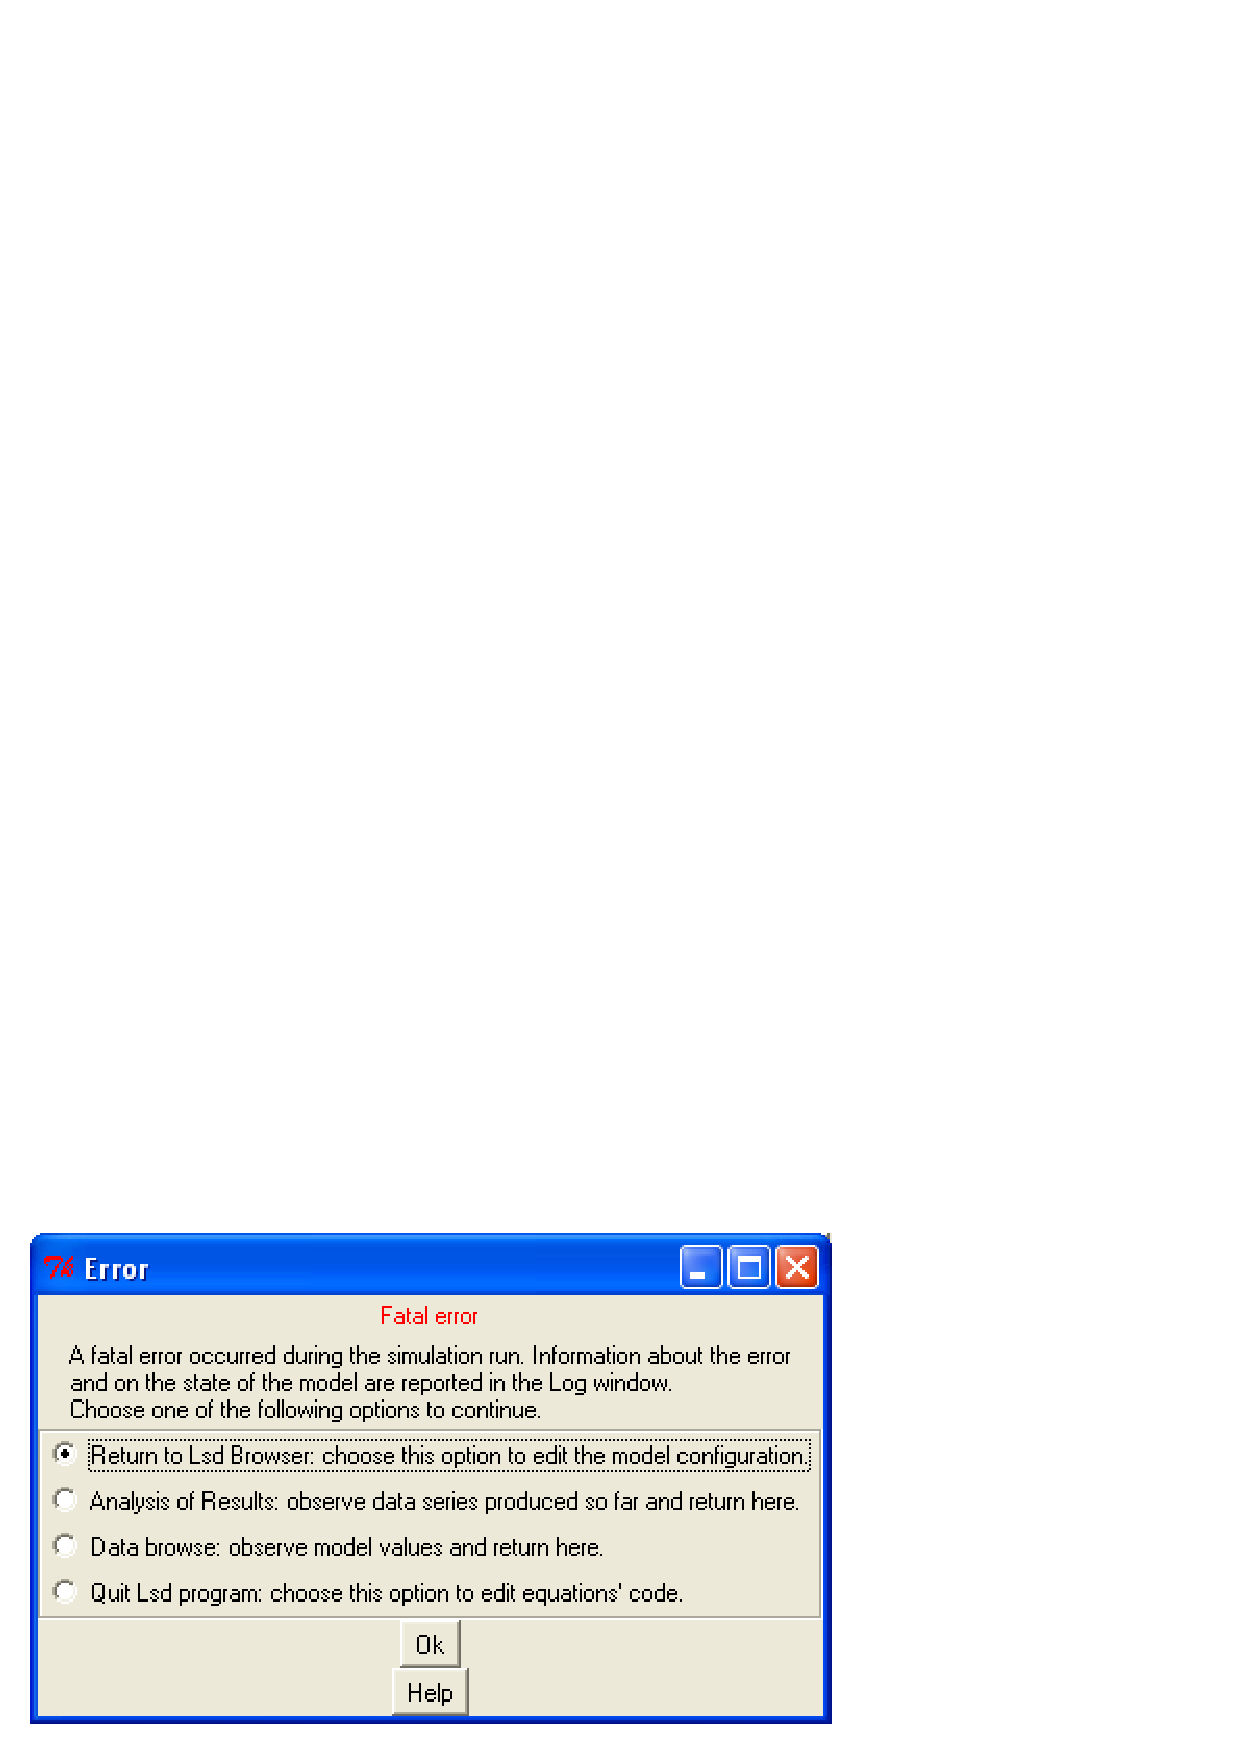
\includegraphics[width=6cm]{abort.pdf}}
  \caption{Simulation aborted for a serious logical error.}
  \label{fig:abort}
\end{figure}

This window tells us that \LsD has encountered a logical error preventing it from
continuing the simulation. This means that somewhere we have written some code for an
equation that is perfectly legal from the computational viewpoint, but, in the 
specific context of model status, prevents to continue the simulation. Let's see now how we must proceed in order to find out
where the problem is.

We may already suspect that the problem lies in the equation for \lsd{RandomWalk}, since
it is after the insertion of this equation that the model failed. However, to be
confirmed on this intuition let's follow the indication of the error window and read the messages
in the log window:
\small
\begin{verbatim}
...

Lag error: Variable RandomWalk requested lag 1 but available only 0

Fatal error detected at time 1. Offending code contained in the
equation for Variable:
RandomWalk

...
\end{verbatim}

\normalsize

The text above says that a ``Lag error'' has occurred concerning the variable
\lsd{RandomWalk}. The second part of the message tells us the time step and the equation
during which the error occurred, confirming our suspects.

The problem is that \LsD tries to save as much memory as possible in order to allow for
simulating very large models for many time steps. When a variable computes its value, the
memory used to store this value is freed when a time step is completed and a new one begins
to be computed. Therefore, if we want to know the value of a variable at time $t-1$ during
time step $t$, we need to explicitly tell the system to maintain the value for one time
step more than the default. 

We should normally do this when creating a variable. If you remember, when adding a
variable to the model we have two fields available: one for the variable's label, and one
for the \menu{Maximum lags used}, which is set to 0 by default. We should have told \LsD
when creating \lsd{RandomWalk} that this variable needs to store 1 lagged value.

We didn't indicate the correct lags for the variable at the time of its creation, so we need to fix this problem. However, at this moment the \LsD model program is in the status of aborting a simulation. The only commands available in this status are shown in the window shown in fig. \ref{fig:abort}. We can:

\begin{itemize}
  \item \menu{Return to \LsD Browser}: return to the Browser, terminating the simulation at this point.
  \item \menu{Analysis of Results}: open the analysis of results window to analyse the data produced so far.
  understand why a model
  \item \menu{Data Browse}: inspect the state of each and every element of the model. This
  functionality (which we still have not explored) allows to understand what is the value
  of each element (even the ones not saved) when the crash occurred.
  \item \menu{Quit the \LsD program}: kill the \LsD model program altogether.
\end{itemize}

Let's return to the browse and re-load the configuration, so that we can edit the new variable increasing the lagged values.
Move the Browser to show the object \lsd{MyObj} and double-click on the variable \lsd{RandomWalk}. We are shown the options'
window; double-click on the label of the variable (in red on the top of the window) and
we have the possibility to modify the nature of this element (see fig.
\ref{fig:edit_var}, pag. \pageref{fig:edit_var}).

Select the option \menu{Variable} and modify the number on the cell after the label \menu{Lags} to 1.
Press \menu{Ok} and you return to the Browser. As you see, now \lsd{RandomWalk} appears
in the list of \menu{Variables} of \lsd{MyObj} with attached the number 1, while \lsd{X}
and \lsd{X1} have 0. This means that \lsd{RandomWalk} is a 1 time step lagged variable.

Before being able to start a simulation run we still have to provide one piece of information. Having added a lag to a variable we need to tell the system which values it needs to use at the very first time step, that is, computing when computing the values $RandomWalk_1=RandomWalk_0+X1_1$. Since there were no time step 0,  these values must be provided by the modeler. They will obviously affect the results, since they indicate the starting point of the random walks. 

$RandomWalk_0$ is an initial value, exactly as any parameter's value. To set this we use
the same interface used to set \lsd{minimum} and \lsd{maximum}: choose \menu{Data/Init.
Values} and you are shown the window to set all the parameters of \lsd{MyObj} plus the
newly inserted variable's lagged value\footnote{Note that if we had defined
\lsd{RandomWalk} having 2 lags (because an equation contained the expression
$RandomWalk_{t-2}$), then we would have two lines in the initial values: one for
$RandomWalk_0$ and another for $RandomWalk_{-1}$.}.

Let' set \menu{RandomWalk -1} to 1000 (use \menu{Set all} for setting all the values in
the 10 copies of the object) and return to the Browser. Double-click on the
\menu{RandomWalk} label in the \menu{Variables} list and set on the options for saving
and debugging this variable.

Return to the Browser and run the simulation (menu \menu{Run/Run}). After that enter in
\menu{Analysis of Results} and plot some time series for the \lsd{RandomWalk} variables
to observe their dynamics. When finished, exit the \menu{Analysis of Results} and, in the
main Browser, re-load the configuration with Control+w.




\section{Multi-layered object structure}

Until now we have worked with a model with only one type of object, \lsd{MyObj}. It is a
``flat'' model, in that every copy of the object works on its own, independently from the
others. However, generally models includes objects at different hierarchical levels.
These ``deep'' models have agents (e.g. firms) interacting via a higher order entity
(e.g. market). For example, a model for a market may contain an object \lsd{Market}
containing, in turn, two types of objects, say \lsd{Demand} and \lsd{Supply}. Therefore,
\lsd{Market} is ``higher'' in the hierarchy, representing a more aggregate element than
\lsd{Supply} or \lsd{Demand}. In turn, \lsd{Supply} may contain several objects
\lsd{Firm}'s, as objects still lower in the hierarchy (i.e. smaller). In this paragraph
we will see how \LsD manages multi-layered models.

Let's modify our model where the \lsd{MyObj} we used so far is contained within
another object in which to compute aggregate statistics, like the average value for all
the random walk variables\footnote{Actually, we already have a higher level object,
\lsd{Root}. But, as already said, it is better to never use \lsd{Root} to contain any element but objects.}. Place the Browser to show the \lsd{MyObj} and then choose menu item
\menu{Model/Insert New Parent}. In the resulting window type the name of the new object,
say \lsd{AggregateObj}. After confirming, verify that your model now includes
\lsd{Root} containing \lsd{AggregateObj} containing \lsd{MyObj}.

If you open now the interface to set the number of copies for the objects (\menu{Data/Set
Number of objects/All types of objects}), you will see that the window shows one copy of the  
the newly created \lsd{AggregateObj} object type. On the right of the line for the new object there is a text signaling that other objects are contained within those objects. Click on the text to ask the system to show the additional objects\footnote{Alternatively, you could type `2' into the entry for the hierarchical level to show and click on \fmenu{Updated}.}. and the window will create a new indented line. 

This new line shows firstly a symbol '\menu{+}', indicating that it is one layer below the objects at the highest layers, conventionally referring to the objects contained in \lsd{Root}. It will then indicate the name of the object the line refers to (in red), and the name of the copy of \lsd{AggregateObj} containing the group for the line. Eventually, we have the number of copies for the whole group, the button labeled with 10.

Click on the red label \lsd{AggregateObj} of the only line for this type of object and type 3 to the resulting window. After the confirmation you will be now shown three distinct groups of \lsd{MyObj}, one for each copy of \lsd{AggregateObj}. Notice that each group has exactly the same number of copies.

\LsD constraints each copy of an element to have all the same structure, although the actual numerical content may obviously vary. We therefore are forced to have at least one descending object \lsd{MyObj} within each copy of \lsd{AggregateObj}. When creating new objects, as we have just done creating 2 additional copies of \lsd{AggregateObj}, the system takes one copy as templar to determine the numerical content (e.g. parameters and number of descending objects) of the new copies. Hence, having only one group, that one had be replicated.

You can change independently the number of copies for each of the groups of \lsd{MyObj}'s contained within each of the 3 copies of \lsd{AggregateObj}, or modify at once all of them. Click on the button with the number 2 of one of the lines for \lsd{MyObj}, for example the second. A new window will appear, like that reported in figure \ref{fig:numobj}

\begin{figure}[ht]
  \centering
 \fbox{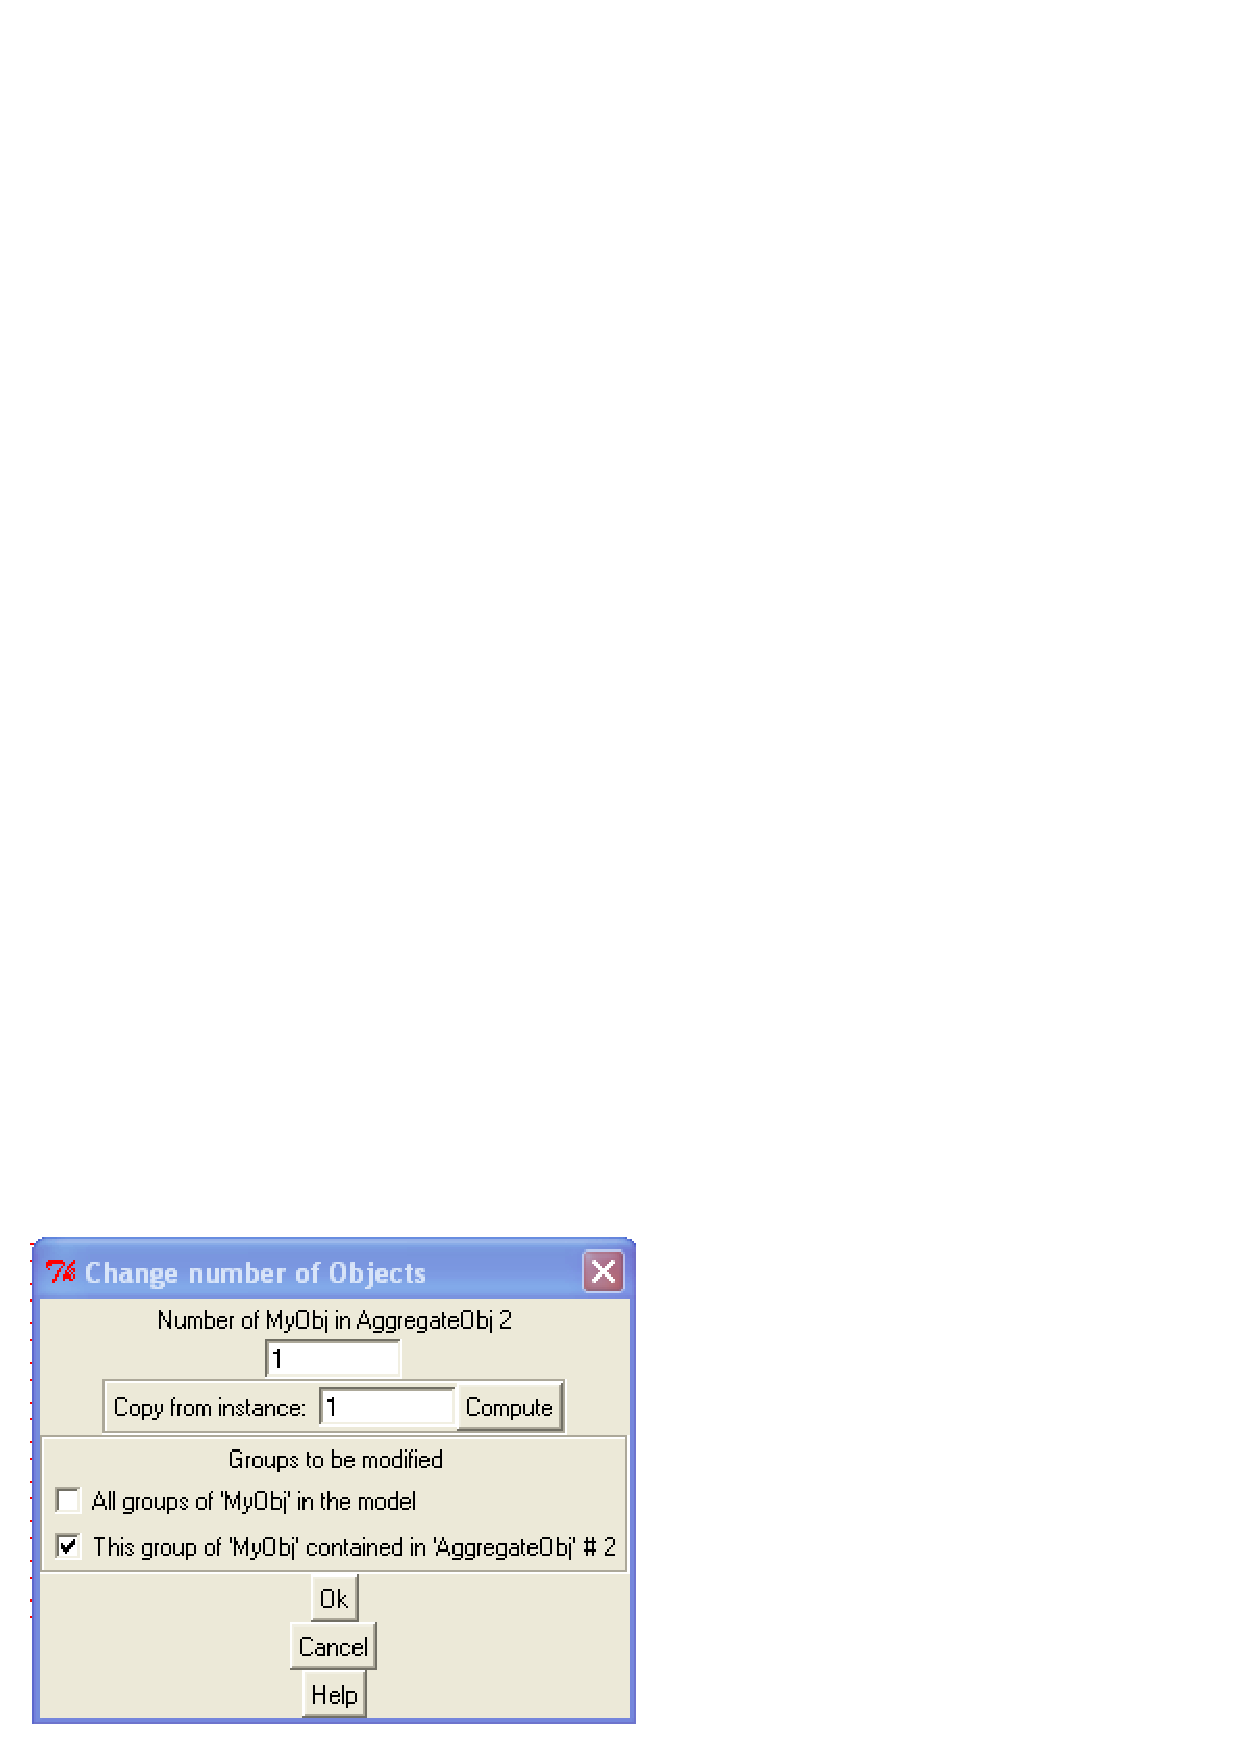
\includegraphics[width=5cm]{numobj.pdf}}
  \caption{Setting the number of descendants. It is possible to modify a single group, or all the groups in the model. Moreover, it is also possible to choose which instance of the existing objects to copy initial values from.}
  \label{fig:numobj}
\end{figure}

This window refers to a specific group of objects \lsd{MyObj}, namely, the group contained in the second copy of \lsd{AggregateObj}. You can decide to modify only the single group of objects, or affect all groups of \lsd{MyObj}. Notice also that when you decrease the number of elements in a single group you have the possibility to decide individually which copy in the group to remove. If this does not matter, by default \LsD will remove the ``leftmost'' objects, that is, the final ones in the group, under the assumption that they are those being added more recently.

Using the features of this window generate three copies of \lsd{AggregateObject} containing 10, 20, and 30
copies respectively. When done press on \menu{Exit} to return to the Browser. Notice how
the graphical representation of the model on the right of the Browser now expresses the
new configuration.

Now that we have created an aggregate object, let's place in it a variable. Put the
Browser on the \lsd{AggregateObject} and add a variable labelled \lsd{AverageRW}
(\menu{Model/Add a Variable}). We need to write the equation for this new variable, and then re-create a new \LsD model program replacing this one. However, for the time being save the configuration (\menu{File/Save}) but keep the program running. It is easier to write the equations having at hand the model structure to visualize. When the equation will be ready we can close the \LsD model program and compile a new one with the new equation.


\section{Equations for multi-layered models}

Back in LMM let's write the equation for \lsd{AverageRW}. The code should simply
implement the expression for the average value of all the \lsd{RandomWalk}, supposing
having n copies of objects \lsd{MyObj}:

$$ AverageRW_t = \sum_{i=1}^n \frac{RandomWalk^i_t}{n} $$

where the index $i$ refers to a succession of copies of the objects \lsd{MyObj}, and $n$ to the total number of copies.

However, in \LsD we don't make use of indexes, nor we need to know the number of copies before starting the computation.  From the programming viewpoint we have the problem of ensuring that each copy of \lsd{AverageRW} is computed using all, and only, the values of \lsd{RandomWalk}
contained in the group of objects \lsd{MyObj} descending from one specific copy of \lsd{AggregateObject}. That is, we want to be sure, for example, that the second copy of \lsd{AverageRW} does not include in the computation values of \lsd{RandomWalk} from objects contained in the first or third copy of \lsd{AggregateObject}. Moreover, when writing the equation, we cannot know how many copies of \lsd{RandomWalk} are used, since
this is defined by the users in the model configuration, and we want our equation to work in general for any number of copies.

The language used for the \LsD equations permits to overcome these problems in a very simple and intuitive way. The operations we are going to write is the computational equivalent of the operations described below. It is anyway necessary define an element of programming language: the \textit{pointer}. Pointers in programming are a special type of variables. A common variable is a label associated to a numerical value, and programmers can assign a value to the variable in a certain line and use this value later on. Pointers have the same function not for numerical values, but for objects: they are variables for objects, but numerical values. Hence, you can assign an object to a pointer, and the use the object \textit{pointed to} by the pointer.

In writing the equations \LsD offers both local variables (\code{v[0]}, \code{v[1]}, etc.) and pointers, called \code{cur}, \code{cur1}, etc. Hence, the pseudo code for computing the average of values in a group of objects is the following:

\begin{enumerate}
  \item define two variables, \texttt{v[0]} and \texttt{v[1]}, both initially set equal to 0;
	\item define a pointer \code{cur} and set it to point to the first \lsd{MyObj} in the group; 
	\item add the value of \lsd{RandomWalk} for the object in \lsd{cur} to \texttt{v[0]};
	\item add 1 to \texttt{v[1]};
	\item are there more objects, after the current one?
  
\begin{itemize}
	\item Yes: replace as \code{cur} the object next to its current copy, and go to step 3.
	\item No: go to step 6.
\end{itemize}
	\item assign to the variable as result the division \texttt{v[0]} / \texttt{v[1]}
\end{enumerate}

In slightly more formal notation figure \ref{fig:cycle} describes the same operations.

\begin{figure}[ht]
  \centering
 \fbox{\includegraphics[width=5cm]{CYCLE.pdf}}
  \caption{Flow chart to compute an average. Command \code{FIRST(cur)} indicates the first object in a group and \code{NEXT(cur)} replaces the pointer pointing to \code{cur} with its following object, like $X_{i+1}$ in respect of $X_i$ with vector notation. }
  \label{fig:cycle}
\end{figure}

The procedure defined by the pseudo-code above computes the average value sequentially, scanning one element per time and cumulating two sets of values for the denominator and numerator of the division.

In \LsD equations commands like this are very frequent, thus the expression is very simplified. The code for the equation is the following:

\small
\begin{verbatim}
EQUATION("AverageRW")
 /* Average value of all the RandomWalk
 values from the descending objects
 */

 v[0]=0; v[1]=0;
 CYCLE(cur, "MyObj")
 {
  v[0]=v[0]+VS(cur,"RandomWalk");
  v[1]=v[1]+1;
 }

RESULT( v[0]/v[1])
\end{verbatim}
\normalsize

Let's see in detail the commands in the code above, keeping in mind that the equation is
computed for a variable contained in \lsd{AggregateObj} and must use the values of
\lsd{RandomWalk} contained in the lower level \lsd{MyObj}.

The first two lines of the code simply set to 0 two temporary variables, which will be
used to cumulate the values of \lsd{RandomWalk}'s and the number of their copies of
\lsd{MyObj}. The actual calculation is done in the command
\code{CYCLE(cur,"MyObj")\{repeated code\}}. This command causes the code contained in the
subsequent group of lines to be repeated again and again as many times as many copies 
\lsd{MyObj} can be found. Notice that the \LsD ``knows'' the object containing the variable that it is computing at any time; call this object the object ``under computation''. \LsD is therefore able, using the command \code{CYCLE}, to scan all and only the objects descending from the object under computation, ignoring the copies contained in other copies of \lsd{AggregateObj}. Therefore the number of repetitions depends on the number of copies of the
objects whose label is \lsd{MyObj}\footnote{If there are no copies of \lsd{MyObj}
descending from the \lsd{AggregateObjext} containing the \lsd{AverageRW} whose equation
is executed the internal calculations in the cycle are never executed.}. During each
repetition the cycle assigns to the pointer \code{cur} a different copy of \lsd{MyObj}. 


In the body of the cycle, that is the code included in between the two curly brackets,
there are two commands. Both commands cumulate numerical values. The second cumulate
simply 1's, so that, after the cycle, \code{v[1]} contains the number of repetitions of
the cycle, that is, the number of copies of \lsd{MyObj}. The first line cumulates in \code{v[0]} a
more complicated stuff: \code{VS(cur,"RandomWalk")}. This command is another form of the \code{V("...")} family, returning the values of elements (i.e. variables or parameters) of the model. The specificity of \code{VS("...")} is that
the programmer must \underline{\textbf{s}}pecify the object where the element is contained.
The difference with the general form \code{V("...")} is that the simple form assumes by default that the object where to search the element to evaluate is stored in the same object\footnote{Within the code for equations modellers can access the object containing the variable under computation, represented by the pointer \code{p}. Therefore, the \code{V(``X'')} is actually equivalent to \code{VS(p,''X'')}.}. 

The general form
\code{V("...")} cannot be used in this equation. In fact, the code for the equation of
\lsd{AverageRW} is executed at level of object \lsd{AverageObj}. In these objects
there is no variable \lsd{RandomWalk} so the system should start a search for an object
containing the desired variable. But all the descending objects \lsd{MyObj} are equally
``distant'' from the object \lsd{AggregateObj}, where the equation for \lsd{AverageRW}
is executed, and therefore the system cannot correctly find any specific copy of
\lsd{MyObj}\footnote{Using \code{V("RandomWalk")} in an equation for a variable in
\lsd{AggregateObj} will return always the value of the very first copy of
\lsd{RandomWalk}.}.

Using \code{VS("...")} instead, we tell the system in which object is contained the
element to compute. We tell the system to use the copy of \lsd{RandomWalk} contained in
\code{cur}, which, through the iterations of the cycle, ``points'' sequentially to all the copies of
\lsd{MyObj} descending from the \lsd{AggregateObj} whose \lsd{RandomWalk} has to be
computed.

Eventually, when the cycle is finished, the equation has scanned every \lsd{MyObj}; for
each of them the equation has added 1 to \code{v[1]} and the value of \lsd{RandomWalk} to
\code{v[0]}, so that we have the denominator and numerator of the division for the
average, which is then assigned as result.


\section{\LsD Simulation Manager}

As we have seen a modeller defines the model structure and the equations, described by chunks of generalized code. However, a program needs a lot more of information to be able to run, determining what the processor must do and when. Users can safely rely on \LsD to fill any explicitly missing information required in order to have a simulation running correctly (i.e. coeherently with the model's definition). In particular, \LsD ensures that the variables' values used in the equations of other variables without lags (and therefore requiring their equations being computed before those where the present-time values are used), are updated in the correct order. Moreover, \LsD ensures that equations making use of elements present in many copies in the model choose the correct values. 

\LsD exploits a default system to ensure that a simulation run performs the most likely operations, though modellers can, if necessary, over-run the default system. In this paragraph we give a hint on how \LsD manages to generate simulation runs out of the information modellers provide. Readers not interested in these technical details can skip this paragraph.

The core of a \LsD model program running a simulation is a system, called \LsD Simulation Manager or LSM. Its task is to assemble all available information concerning the model and produce an actual simulation run\footnote{Or, in case of errors, interrupt the computation, avoid program crashes, and provide as much information as possible concerning the problem encountered.}.

A simulation run is a sequence of time steps, within each of them all the variables must be updated (i.e. their equation executed) according to a specific order, that is, for example, which equation must be executed at the beginning of the time step and which can be executed at the end. The order of updating is important, since it determines whether the values of a variable used within the equation for another variable are those from the previous time step or those from the current one, and, in general, the results obviously differ.

Some simulation languages requires modellers to define explicitly a \textit{scheduler}, that is, the ordered list of equations to be executed within a time step. \LsD uses a different approach, generating on the fly the schedule of the execution of equations by analysing the implicit temporal constraints as can be deduced from the very code of the equations. For this operation the LSM makes use of two bits of information: the general clock of the simulation run (called \code{t}) and a field contained in each copy of the variables indicating what was the simulation time when the variable was lastly computed, a field called \code{lastupdate}.

Let's see how the LSM exploits this information to ensure the correct schedule of updating within a simulation step. At the start of a simulation step the first operation performed by the LSM is to increase the time counter of one unit. After that the LSM begins scanning all the objects in the model and, within each of them, controls all the variables contained. For every variable considered the LSM compares the simulation clock with the field \code{lastupdate} of the variable. If these values are different (that is, \code{lastupdate} is smaller than \code{t}) than the clock, then the LSM begins the execution of the equation for that variable, otherwise (\code{lastupdate}=\code{t}) it skips the variable and moves to the next one.

While executing the equation for a variable the code may require the value of other variables in the model, typically through the command \code{V(...)}, as happens in the computations for \lsd{X1}, \lsd{RandomWalk} and \lsd{AverageRW} in our example model. If the values of the variables is requested with a lag, then the system can use the value as inherited from the previous time step. Otherwise, if the variables are requested as values computed at the present time, they may have it  or not. 
 
The LSM is able to distinguish this cases, comparing the lags of the values required in the equation's code, with the time clock of the simulation and the \code{lastupdate} field of the variables concerned. When a requested variable's value is available LSM returns the value to the equation under computation directly.  When the value necessary to continue the computation of an equation is not available, it means that the variable did not computed its equation at the current time step as yet. In other terms, the scheduler should have computed firstly that equation, and later the one it (erroneously) has already started. In this case the LSM ``corrects'' its mistake by interrupting the computation of the variable to the stage it already reached, and moves to execute the equation for the required variable. When that computation is completed, it then returns to the interrupted equation, provides the updated value of the variable, and continue the computation. When the computation for the equation is terminated, and the resulting value stored in the variable, its field \code{lastupdate} is updated in line with the clock of the simulation.

Note that the system may iteratively continue for several cycles: even the newly computed equation may require, in turn, other values not yet available. LSM can generate, if necessary, a long chain of half-computed, interrupted equations until it manages to compute the last one, and then rolls back all the interrupted computations completing them in reverse order.


Notice that the way the LSM arranges the order of completion of the equations is independent of the order for the starting the computations of the variables. Therefore it is possible to use any rule for scanning the variables of the model; in practice, \LsD begins by (trying to) compute firstly the variables in the higher object (\lsd{Root} is always the first). When the scanning encounters a variable that have been already updated, because another variable requested its new value, it does not re-compute equation.

An important property of the LSM is that the actual order is decided at run-time. There may be cases where a variable's equation contains two alternative computations (distinguished by an \code{IF ... THEN ... ELSE} command), requiring two different order of updating conditional on certain events. The LSM will automatically generate different schedules of updating, depending on which condition applies at every step.

For a similar reason, LSM guarantees that the code for equations can easily be moved across different models. Depending on the equations for the variables within an equation, different models will generate different schedules, without the necessity for the users to pay attention to the schedule.

The LSM allows also to modify, possibly heavily, the schedule of a model in an extremely simple way. For ensuring that one computation (e.g. for variable \lsd{Z}) takes place before the completion of another variable (say \lsd{Y}), it is sufficient that the very first line of the code for the equation of \lsd{Y} contains the command \code{V(``Z'')}. The LSM ensures that any computation occurring after that line, variable \lsd{Z} will be updated, that is, its computation already performed.

Lastly, LSM is able to spot inconsistencies in the model, avoiding never ending cycles where one or more variables require both to be computed before the other. For example, the ``models'' made of two equations: $X_t=Y_t$ and $Y_t=X_t$ is not computable, in that it would generate an infinite bouncing between the two equations. As we will see the LSM identifies this potentially fatal errors and issues messages helping the modeler to fix the problem.

The equations we have written for our example model are the computational translation of a difference equation model that may be expressed with the following equations:

\begin{equation}
\begin{tabular}{ll}

$ \textnormal{AverageRW}_{t}^i$ & = $\displaystyle \sum_{h=1}^{n_i} \frac{_{t}\textnormal{RandomWalk}_t^{i,h}} {n_i} $\\
$ \textnormal{RandomWalk}_t^{i,j}$ & = $\textnormal{RandomWalk}_{t-1}^{i,j} + _{t}\textnormal{X1}_{t}^{i,j}$ \\
$\textnormal{X1}_t^{i,j} $& =$ \textnormal{minimum}^{i}+(\textnormal{maximum}^{i}-\textnormal{minimum}^{i})\textnormal{X}_{t}^{i,j} $\\
$ \textnormal{X}_{t}^{i,j} $& $ = r.v. U(0,1) $ \\
\end{tabular}
\end{equation}



The \LsD representation for these equations, as we have seen, can neglect the time suffix $t$, which is redundant (but includes the lag indication), and relies on the model's structure of objects instead of
using the impractical and error-prone indexing system. In the rest of this paragraph
there are some further details on how \LsD replaces the indexing system.

 In our case, as in practically any model, there are many copies for each variable, one in each copy for any 
type of object. Every copy of the same type of variable executes the same computations, though, obviously, make use of different values. For example, every copy of \lsd{RandomWalk} needs its own lagged value
and its own copy of \lsd{X1}.

\LsD manages to obtain this by using an information stored into the variables: which object contains it. When the
equation is activated all the \LsD functions, like \code{V("...")}, ``know'' the copy of
the object containing the variable whose equation is executed. This bit of information is
available to the modeller, too, as the object pointer (i.e. the C++ variable storing
objects) called ``\code{p}''. For example, the expression \code{V("X1")} is equivalent to
the expression \code{VS(p,"X1")}. In the former case we rely on \LsD to find out the
correct copy of \lsd{X1}. The system is executing the equation for \lsd{RandomWalk} in
some copy of \lsd{MyObj}, so that \code{V("X1")} will return the value of \lsd{X1}
contained in the same object. Instead, in the second case, using \code{VS(p,"X1")}, we
tell the system to return the value of the copy of \lsd{X1} in \code{p}, which is the
same copy of \lsd{MyObj} containing the copy of \lsd{RandomWalk} under computation.

In practice, \LsD dispenses from the use of indexes by using the more flexible concept of ``membership'' to an object. If a variable's equation requires another element the system will provide the copy of the element contained in the same object or, if it is not there, in the ``closer'' object containing the variable under computation. This system ensures that modellers can avoid to specify exactly where each element can be found, and also allows to use the same code of an equation in different model structures, where the same elements are stored in different objects.

This automatic system to retrieve elements system is useful most of the times, but not always. There are cases where the modeller needs to indicate in an equation a specific copy of an element chosen according to elaborated rules. For these cases \LsD provides a set of functions allowing modelers to express any possible strategy.


\section{Extending the model: quality and sales }
We are proceeding gradually adding new equations one by one. This style of proceeding is highly valuable in avoiding ``complexity traps'' generated when one tries to write a complete model before testing any of its components. \LsD favors this style since the simulation program ``adapts'' the simulation run by itself, depending on new elements introduced, changes in the lags of existing variables, etc. Given the speed with which a run can be produced, possible corrected, and analysed, it is possible to test the effects (and the correctness) of each and every variable added to the model.

For the moment we have implemented just a set of random variables that independently create a set of random walk
processes, and we have computed an average of these processes. Let's interpret this model
as a metaphor for (very simplified) processes of technological improvements.

That is, we interpret one \lsd{MyObj} as a firm performing R\&D whose result (totally random)
is a quality level for its product (the \lsd{RandomWalk} variable). We want to link the
relative quality of each firm (relative to the average quality) to the level of sales.
In practice, we need two new variables, and their equations, expressing an indicator of competitiveness based on the quality of the firms, and the levels of sales. In formal terms the
equations are:


\begin{tabular}{ll}\label{eq:relativequality}

$RelativeQuality_t=\displaystyle \frac{RandomWalk_t-AverageRW_t}{AverageRW_t}$
\\
$ Sales_t=Sales_{t-1}(1+alpha*RelativeQuality_t)$

\end{tabular}

The variable \lsd{RelativeQuality} should not pose any problem of interpretation. If a
firm (i.e. \lsd{MyObj}) has a quality level (i.e. \lsd{RandomWalk}) identical to the
average of all firms, then its relative quality is null. If it is higher than the average, its relative
quality is positive, boosting its sales, otherwise it is negative, decreasing sales.

The second equation states that the level of sales for a
firm is inertial, changing slowly in the the direction of the sign of relative quality. The equation
says that the value of sales at any time step equals its previous value plus a share
(\lsd{alpha}) which is added or removed depending on the relative quality. 

Note that the equation for sales relates sales rate of changes to the relative quality. The absolute level of change in sales depends also on the past level of sales.

Let's see the equation's code for \lsd{RelativeQuality}:
\small
\begin{verbatim}
EQUATION("RelativeQuality")
/*
Compute the relative quality
of a firm as the relative ratio
of the difference between RandomWalk
and AverageRW
*/

v[0]=V("RandomWalk");
v[1]=V("AverageRW");

RESULT( (v[0]-v[1])/v[1] )

\end{verbatim}
\normalsize

There is nothing new in this equation, but it is worth noting something we still
did not meet in our model. \lsd{RelativeQuality} is a variable stored in \lsd{MyObj}.
Therefore, the \code{V("RandomWalk")} expression returns the value in the same copy of
\lsd{MyObj} containing the copy of \lsd{RelativeQuality} executed. But what about
\code{V("AverageRW")}? This is a variable contained in \lsd{AggregateObj}
that is in an object ``higher'' than the one where the equation is executed, \lsd{MyObj}.
How does \LsD manage this situation? Assuming the obvious: the copy of \lsd{AverageRW}
returned in each equation is the one contained in the \lsd{AggregateObj} copy
containing the copy of \lsd{MyObj} whose \lsd{RelativeQuality} is executed. This
automatic retrieval of data in ``higher'' objects is possible because \LsD models are
strictly hierarchical, so that a lower level object is directly linked to only one higher
level object.

The second equation's code does not pose any particular problem of interpretation:

\small
\begin{verbatim}
EQUATION("Sales")
/* Compute the level of sales as the relative
growth proportional to alpha of the
relative quality */

v[0]=VL("Sales",1);
v[1]=V("RelativeQuality");
v[2]=V("alpha");
v[3]=v[0]*(1+v[2]*v[1]);

RESULT(v[3])
\end{verbatim}
\normalsize

Now we can compile the model and, if there are no grammar error in the equations'
code\footnote{If there are errors, choose not to run the existing \LsD model program and
see the second line in the window \fmenu{Compilation Results}. There should be a line number, indicating
approximately where the error has been found.}, we can use \LsD model program to make the necessary modifications to the configuration of the model:


\begin{enumerate}

\item load the configuration file (\menu{File/Load});
\item move the Browser to show the object \lsd{AggregateObj};
\item add the parameter \lsd{alpha} (\menu{Model/Add a parameter});
\item initialize the parameter to 0.2 (\menu{Data/Init. Values});
\item move the Browser to show the object \lsd{MyObj};
\item add the variable \lsd{Sales} (\menu{Model/Add a variable}, indicating
that it uses 1 lagged value);
\item add the variable \lsd{RelativeQuality} (\menu{Model/Add a variable});
\item initialize the values in \lsd{MyObj} (\menu{Data/Init. values}) setting all
the \lsd{Sales}' values to 1000.
\end{enumerate}


Before running a simulation double-click on the labels for \lsd{Sales} and
\lsd{RelativeQuality} setting on the option to save the variables' values, so that we
will be able to analyse their values after the simulation run.

If there are errors appearing after the simulation has been launched, chances are that
you misspelled some of the newly inserted variables or parameter. Remember that elements'
spelling must be identical in the \LsD model configuration and in the equation file. If
you have an error, check in the \menu{Log} window which element could not be found by the
system. When a mis-matching error occur you may need to change either the label in the code of the equations or the label in the configuration. 

Another frequent error by beginners is to forget that \LsD model programs cannot execute the code of the equations merely because it has been written. After coding new equations, the modeler needs to shut down the existing \LsD model program and compile a new one. Only after a re-compilation the code for the new equations can be exploited. 


\section{Assessing the model's behaviour}
Let's see how the model behaves. First of all we need to configure the initial values in
a sensible way. Set the number of \lsd{AggregateObj} to 1 containing ten copies of
\lsd{MyObj}, and the \lsd{alpha} parameter set to 0.2. Set the values for parameters
\lsd{minimum} and \lsd{maximum} are all set to -10 and 10 respectively. This ensures that
the random walks are centered on 0 without systematic biases. Finally, set the all the
lagged values for \lsd{RandomWalk} and \lsd{Sales} to 1000, assuming identical initial conditions for all the firms in the model.

Any user of \LsD running this model with the above initialization will produce exactly the
same results. For example, in figure \ref{fig:relqua} it is reported the series for the
relative quality levels over the first 100 time steps.

\begin{figure}[ht]
  \centering
 \fbox{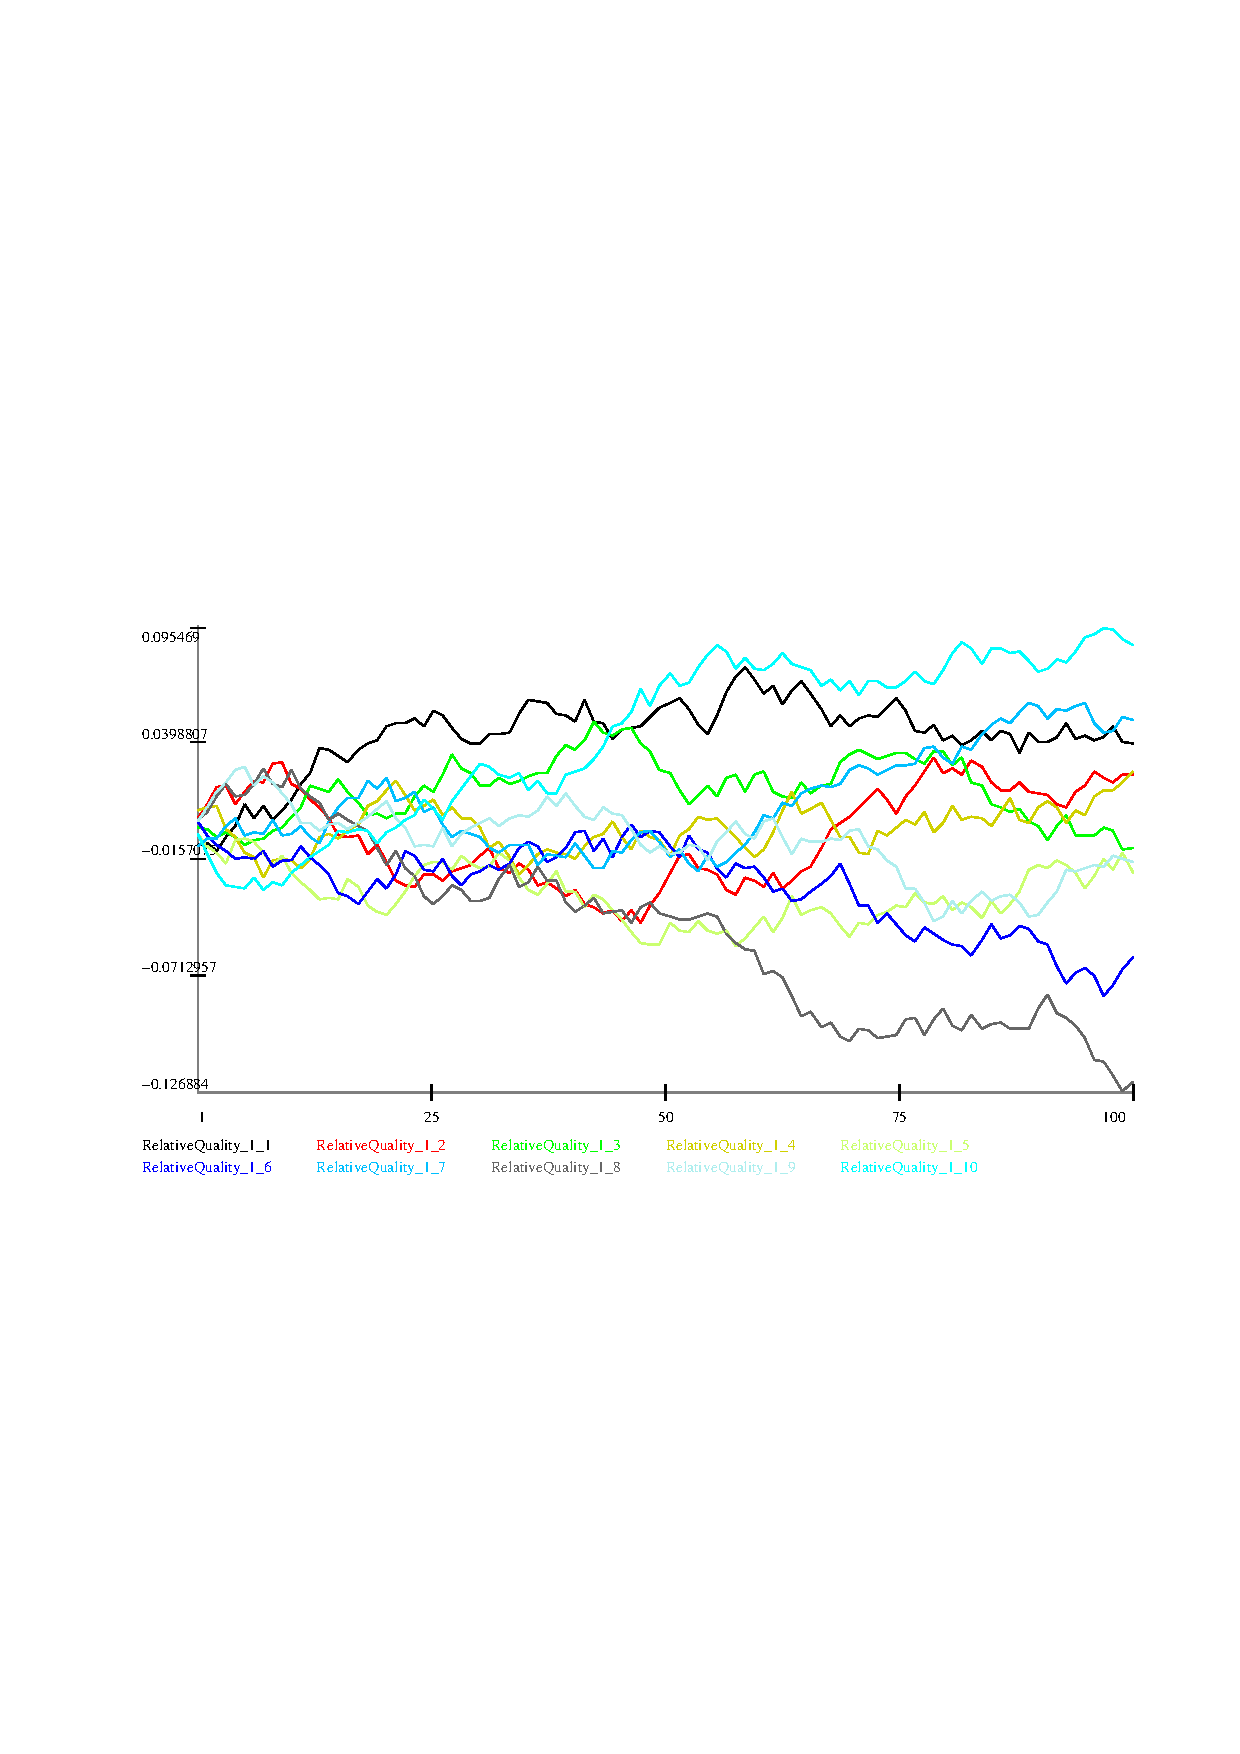
\includegraphics[width=10cm]{relqua.pdf}}
  \caption{Relative quality over time steps from 1 to 100.}
  \label{fig:relqua}
\end{figure}

One may wonder how it is possible that supposedly random events happen identically on any
computer run. This is one of the advantage of using simulations. You do have random
events, but you can re-run a simulation using exactly the same set of (pseudo-)random
events so as to control exactly what happened during (pseudo-)stochastic events. If you want, as usually is the case, to run the same simulation (i.e. same initialization) with different random events, then you
need to change the \code{seed} value, which is set in menu \menu{Model/Sim.Setting}.

We can control whether the model produces, as expected, a relation between the values of sales and \lsd{RelativeQuality}. In Analysis of Results select all the \lsd{RelativeQuality} and all the
\lsd{Sales} series. Then check the options for \menu{Cross Section}, \menu{XY plot}, \menu{Points}, and
press \menu{Plot}. The new window appearing will ask which time step you want to consider the data, besides other options. Leave the existing default value and press \menu{Ok}. The resulting graph will show the points whose coordinates are given by the values of the couples of \lsd{RelatieveQuality} and \lsd{Sales} for each \lsd{MyObj} at time step 100. As we can see, the points indicate a roughly increasing relation, as expected.

Is this model a good representation of the purported effect of quality on sales? If we analyse the model results we see that, actually, something is wrong, if not technically (the model does exactly what we told it to do), but the ``scientific'' interpretation of the results is inconsistent.

In fact, the equation for sales is implemented as a function of the \textit{relative} quality, in that, implicitly, we would like to have some firms increasing their share of the market and some decreasing them. This representation would implicitly suppose that the total level of sales, the dimension of the market, would remain constant. Is this the case?

Though a mathematically skilled reader would immediately induce the answer from the functional form of our variables, the laziest may instead prefer to exploit the model to investigate the matter. For example, we may try to generate the increments in sales of the different firms, $DiffSales_t=Sales_t-Sales_{t-1}$. We know how to introduce and write the equations for such a variable. However, let's use another way, to introduce a new command for the writing of \LsD equations.

When the model computes the level of sales we already have available the past level of sales, so that we may directly compute the values for the variable we are interested, call it \lsd{DiffSales}, during that computation. Though \LsD forces the code for a variable to generate only one single result, it is possible to use a special command to write values on any element of a model. Consider this modified code for the equation for \lsd{Sales}:

\small
\begin{verbatim}
EQUATION("Sales")
/* Compute the level of sales as the relative
growth proportional to alpha of the
relative quality */

v[0]=VL("Sales",1);
v[1]=V("RelativeQuality");
v[2]=V("alpha");
v[3]=v[0]*(1+v[2]*v[1]);

WRITE("DiffSales",v[3]-v[0]);

RESULT(v[3])
\end{verbatim}
\normalsize

The new version of this variable does not modify the result produced by for the variable \lsd{Sales}. But, although obviously an equation can return a single value for its variable, the code for the equation may contain any C++ (and \LsD-specific) statement. In the above example we requested the equation for sales to write a value (the difference between the lagged and current sales) onto an element of the model, called \lsd{DiffSales}. We can now introduce a parameter in \lsd{MyObj} labelled \lsd{DiffSales} that will contain the sales' differences for each firm in the model.

It is worth to notice that the use of a \code{WRITE} command is, in general, non necessary, since a variable with a specialized equation may do the same job. Generally, the reason for using the command \code{WRITE(...)} is to speed up the implementation of the model, or the execution of simulation runs. This command needs also to be used with caution because it does not allow the automatic management of updating. In fact, being a parameter, \LsD does not ``know'' the time when \lsd{DiffSales} is written; therefore, if the model were to use the value of \lsd{DiffSales} in other equations, it would be necessary to manually ensure that the values are used in the correct way (before or after it is updated by equation for \lsd{Sales}). In our case we do not run any risk, since the parameter is used only for statistical purposes and does not affect other results of the model. 

Let's compile the new simulation model program and load the existing configuration. Move the Browser to show the object \lsd{MyObj} and add the parameter \lsd{DiffSales}. You need to open the interface to initialize the elements of these objects (menu \menu{Data/Init. Values}) because, being a parameter, \LsD requires it to be initialized, even though the initial values are never used in the model. Just open the initilization window and close it, which is sufficient to signal that the default value (zero) is accepted by the user. Remember also to check on the option to save these values, by double-clicking on its label in the Browser.

\section{Generating new series} 
Run the simulation and open the Analysis of Result module. You will find the series for the new parameter \lsd{DiffSales}; select them and plot their results after having reset the options to the default values (\menu{Time Series}, \menu{Lines}, \menu{Sequence}). If the assumption that any increase in one firm's sale should be matched by an equal decrease by other firms' sales were true, the average value of \lsd{DiffSales} across all \lsd{MyObj}'s should be null. Is this the case? The graph is not conclusive in this respect, so we need to find a more precise tool. We may re-run the same simulation adding a new equation computing the average, but here we use a different method: generation of new series from those saved in Analysis of Results.

The module we use so far only to to show the results saved from simulation runs has the possibility to create new series from manipulating the available series. Clicking on the \menu{Add Series} button in between the two main listboxes list the possibilities offered to add new series. Choose the option to \menu{Create one series ...} and you will be shown a window as in figure \ref{fig:elab}.

\begin{figure}[ht]
  \centering
 \fbox{\includegraphics[width=4cm]{elab.pdf}}
  \caption{\small Generate new series as elaboration from the currently selected ones. The new series will appear as a single statistics computed over time (first option on the top) or across series (second option). Choose the statistics to be computed, the name of the new series and a tag index to be used.}
   \label{fig:elab}
\end{figure}

Leave the first option selected to generate a series across times steps. Choose \menu{Sum} as elaboration. Note that the label text reflect the origin of the series and the elaboration chosen (you are free to change it). Pressing \menu{Ok} the new series will be added to the list of available series. Empty the central list and plotting a graph of this new series; it will be obvious that the sum of the differences is not null across the simulation steps, and therefore we need to modify the model if we want to force the dimension of the market simulated in our model to remain constant.

\section{Replacing a variable}

Given our interpretation of sales improving according to the relative quality in respect
of the average, what we need to change the way the average is computed. The simple
average we have used so far considers all firms as equally important. Instead, if we want
to interpret this average as an indication of the average quality for a general consumer, we need to ensure that the individual firms' qualities are compared with the \emph{weighted} average of qualities, where the weights are given by the level of sales.

In the next paragraph we will implement the weighted average, and we will discover an
unexpected error, and the tools to fix it offered by \LsD.

The equation for a weighted average is simply:

$$WAverageRW_{t}=\frac{\displaystyle
\sum_{i=1}^nRandomWalk_{t}^i*Sales_{t}^i}{\displaystyle\sum_{h=1}^n Sales_{t}^h}$$

This expression guarantees that firms' qualities with higher sales levels ``count more''
than firms with lower level of sales. Consequently, we will not observe an absolute
growth of the total level of sales, but only a different distribution of a constant
amount. More on this when we will be able to run the model. 

The code for \lsd{WAverageRW} is:

\begin{minipage}[h]{10cm}
\small
\begin{verbatim}
EQUATION("WAverageRW")
 /*
 Weighted average value of all the RandomWalk
 values using Sales as weights
 */

 v[0]=0; v[1]=0;
 CYCLE(cur, "MyObj")
 {
  v[3]=VS(cur,"Sales");
  v[2]=VS(cur,"RandomWalk");
  v[0]=v[0]+v[2]*v[3];
  v[1]=v[1]+v[3];
 }

RESULT( v[0]/v[1])

\end{verbatim}
\normalsize
\end{minipage}


In order to use this new variable, we need to upgrade the equation for
\lsd{RelativeQuality} (see the equation's code in paragraph \ref{eq:relativequality} at
pag. \pageref{eq:relativequality}). In the equation replace the line:

\begin{verbatim}
...
v[1]=V("AverageRW");
...
\end{verbatim}

with

\begin{verbatim}
...
v[1]=V("WAverageRW");
...
\end{verbatim}

Compile and run the \LsD model program (\menu{Model/Run}). Load the configuration and move
the browser in \lsd{AggregateObj}. Here add the new variable \lsd{WAverageRW}, and set its options so that to save it for post-simulation analysis. We are now ready to run the simulation, but the an error message will soon appear.

\section{Dead-lock errors - Spotting and fixing temporal inconsistencies}

The simulation aborts immediately. Writing simulation models, like
any computer program, is prone to two types of errors: firstly, we may write
\emph{grammar} errors. These errors, that you are likely to have already experienced, are
mistakes in the code such that the compiler cannot understand the commands in the code, since they do not respect the grammar of the language used. Typically, you can mistype a command or forget the semi-colon at the end of a line. These errors are recognized at compile time, and they need to be fixed before the program is created.

The second type of errors concerns grammatically correct code, that the compiler can successfully interpret, but
that implements illogical or inconsistent commands. This is what happened to our upgraded
model: the \LsD model program has been created, because the commands were correct, but
during the actual simulation run \LsD realised that there is an inconsistency. Let's see
firstly what a dead lock error is, then we analyse the information provided by \LsD to
find the cause of the error, and, finally, we will fix our model.

The dead lock errors are cycles of computations that the computer is not able to resolve.
They are the equivalent of asking a computer to solve the chicken-egg problem by brute computational force, and the machine applying its typical mechanical attitude of actually trying. 

As an example of a dead-lock error, consider a set of three variables with their equations, each using one of the other variables:

  \begin{eqnarray}
    X_t = f_X(Y_t) \nonumber  \\
    Y_t = f_Y(Z_t) \nonumber\\
    Z_t = f_Z(X_t) \nonumber
  \end{eqnarray}

One of the basic concepts in computing is that of subroutine. They are parts of code that
execute specific operations, for example computing a number as elaboration of other
values. If a subroutine requires a value which is still not available, the program
interrupts its current operation (remembering at which point it was interrupted and any
intermediate result obtained so far) and executes the subroutine for the requested value.
When the subroutine has finished, the initial operations can continue using the result provided by
the subroutine.

Let's see how this work in the example above. Suppose to start trying to compute firstly $X_t$ (though the same
applies starting from $Y$ or $Z$). The equation for $X$ starts to be executed, but its
complete computation requires the value of $Y$. Therefore, the computer interrupts the
execution of $f_X$ and begins computing the equation for $Y_t$. Also $f_Y$ cannot be
completed because it requires a value not yet available, $Z_t$, and therefore also the
equation $f_Y$ is interrupted and the computer begins to compute $Z_t$ using its equation
$f_Z$. But one of the values to be used in this latest equation is $X_t$, whose equation,
though initiated, still did not provide the value for $X_t$. Therefore, following blindly
the rules of computing, the processor would start to compute the equation $f_X$, which is
interrupted in order to compute $Y_t$, etc. ...

In ancient operative systems a circular set of subroutines like this used to freeze
computers because the processor initiated to compute each subroutine without being able
to finish any computation, and refusing to accept commands from the keyboard (therefore
the name). Modern operative systems avoid to lock computers, but the program entering in
this sort of errors crashes without any notice, making impossible for the programmer to
spot the faulty lines in the code. \LsD recognizes  dead locks before the operative system
and interrupts the simulation providing all the information required to fix the error.

Before continuing to analyse the \LsD tool kit for fixing dead lock errors, let's make a
brief comment on dead lock errors. Simulation programs are not mathematical but
computational logical structures, and this is nowhere clearer than in the case of dead
locks. A mathematical model can well contain a set of equations as in the example above.
In mathematical terms those set of equation is interpreted as: \textit{the set of value(s) of X, Y and Z such that the three equations $f_X$, $f_Y$ and $f_Z$ are all satisfied}. In other terms, mathematics interpret a set of equations as conditions, or constraints, to be satisfied, without any indications on how the variables may be computed.

On the contrary, in computational terms a set of equations is interpreted as instructions to be executed, computing the values on the right-hand side of the equation to be stored in the variable indicated on the left-hand side, without any prior indication of the properties of the outcomes of those computations

The difference between computing and mathematics consists in the symbol ``=''. In mathematics it is the condition such that the values on both sides of the equation are identical. In computing, instead, ``=''
means that the variable on the left of ``='' must assume the value on the right.
Therefore, for example, in mathematics you can never write $X=X+1$, since there is no
number equal to its subsequent. Instead this is perfectly legal in computing: the
command assigns to $X$ its own value plus one. Conversely, in mathematics you may write
$X+Y=2$, but it makes no sense in computing, since there is no variable on the left to
which assign the value. Note that, in programming languages, you always have two
different symbols for assigning values to variables (e.g. ``='' in C++) and for testing
the condition on whether two values are identical (``=='' in C++).


So, the main problem with dead lock errors is to identify the chain of equations that,
calling each other, caused the never ending cycle to occur. Let's see the information \LsD
gives us to find out what type of error is and how to fix it. They are contained in the
\menu{Log} window of the \LsD model program. The messages you find consist in several
lines providing information on the status of the model when the error occurred. The
crucial lines are the last ones. In our case these lines are:

\begin{verbatim}
Level   Variable Label
3   RelativeQuality
2   Sales
1   WAverageRW
0   \LsD Simulation Manager

\end{verbatim}

They indicate that the model has started the simulation (level 0). The \LsD Model Manager began the updating of the variables in the model, trying to compute the variable \lsd{WAverageRW} (level 1). This computation was
interrupted in order to obtain the required value for \lsd{Sales}, whose execution
started at level 2. But also the equation for \lsd{Sales} needed to be interrupted in
order to compute first the value of \lsd{RelativeQuality}. Up to here the system worked
normally. In fact, at any time step \LsD tries to compute the new values for each and
every variable in the model, starting from the ones in the top level objects. If their
equations require updated values from variables not yet updated, then it interrupts the
current computation in order to execute first the variables required\footnote{Each
variables is tagged with the time when it was lastly computed. Therefore, it is frequent
the case that one variable is firstly computed because requested by another equation. If,
in the same time step, its value is requested again, its equation is not re-executed, re-using the previously computed value.}. In programming jargon, when a subroutine, like
the equation for a variable, is interrupted in order to compute another subroutine, you
say that it is ``place on the stack''. The level indexes in the \menu{Log} message
concern the ``stack levels'' at which an equation is executed.


In our case, the error is caused by the fact that the equation for variable
\lsd{RelativeQuality} requires the present value of WAverageRW, which cannot complete its
computation. Here the system realized that a dead lock risked to be initiated and issued
the error message, blocking the simulation.


Now we know what is the error in our model: the average quality indicator uses the value
of sales which is a function of the relative quality, which, finally, requires the weighted
average quality. Since all these variables must be computed by their respective equations
before being used, the system does not know how to solve the circularity of the commands
contained in the equations' code. It is up to us, as programmers, to find a solution. The obvious one consists in changing one of the equations involved using a lagged value for one of
the variables. The variable to choose is not important from the computational viewpoint,
but depends on the interpretation of the variables. The most logical option, in our
example, may be to change the equation for \lsd{RelativeQuality} in order to make use of
the past values of \lsd{RandomWalk} and \lsd{WAverageRW}. In this case, we tell the model
that the relative quality of today (time $t$) is a function of the relative qualities of
yesterday ($t-1$), inserting a lag in the response from quality (\lsd{RandomWalk}) to the
relative quality.


Having understood the error, and found how to fix it, we need to change the equations'
code. Firstly, however, we need to kill the \LsD model program that, though the simulation
is blocked, is still running. The program offers four options:

\begin{itemize}
  \item \menu{Return to \LsD Browser}: return to the browser as if the simulation was terminated normally.
  \item \menu{Analysis of Results}: move to analyse the results produced so far.
  \item \menu{Data browse}: show every copy of the objects in the model, and every element within them.
  \item \menu{Quit \LsD model program}: kill the \LsD model program.
\end{itemize}

In our case we don't have data to analyse, because the simulation crashed at the very
first time step. Also the \menu{Data browse} option is not useful, since the error does not
depend on the values produced in the simulation. Therefore, we kill the program clicking
on \menu{Abort} and return to LMM in order to fix the equation for \lsd{RelativeQuality}.


\section{Modelling Time: changing order of \LsD equations}

What we need to do in order to fix our error is simply to switch the order in which the
equations are executed within a time step: first relative quality, and then average
quality. It requires few changes to the equations' file, that we will see in a moment.
Firstly, however, it is worth reasoning on what we have discovered by means of the dead
lock error, and how to go to fix it.

There are two ways to see this: a mathematician, or a modeller used to standard
analytical models, may see this as an annoying quirk required by the stupidity of
computers, unable to solve even the simplest set of linear equations. Under this view, a
dead lock error, and the way to solve it, is only a technical problem. The opposite way
is to interpret the discovery of a dead lock error as an improvement of our knowledge of
the modelled phenomenon. In fact, normally people represent to themselves a model by
individual variables, and equations, neglecting the overall temporal or logical pattern
linking the variables to form the overall model. Actually, this is the very reason for
using simulations: I tell the computer how to compute X, Y, Z etc., and then observe 
to their joint effect through time. The fact that a dead lock error occurred is a signal not much (and not necessarily) that your individual equations were wrong in the first place, but that the system as a whole was incoherent. And this is a potentially useful result: however negative, acknowledging an error is the first step to solve it. 

Most of the times, dead lock errors point to missing conceptual elements of the model,
which is well worth to analyse. For example, consider a model where a set of firms decide
the quantity to produce as a function of the market price, and the market price is a
function of the quantity produced. Besides the functional forms, the model is still not
complete: I need to specify whether firms decide firstly their production as a function
of past price, or if the price is computed first as a function of past quantities.
Generally, I will obtain different results in the two cases, since they assume different
types of behaviour by consumers and producers. A dead-lock error, in this case, shows that a missing part of the
model needs to be filled. This is an example of why simulations are a useful analytical
tool: being forced to think how to implement consistently a given phenomenon, modelers are forced to
devise rigorous algorithms, and therefore to have a precise idea on how the world really
functions. And one of the undeniable properties of real-world events is that they take place in real time, and therefore the timing of the simulated events have a relevance, as much as the timing of real-world events is important. In practice, finding a solution to a dead-lock error is not a difficult problem, considering how real-world examples actually function. 

In our case we can easily solve our the problem by modifying one of the three equations concerned with the error, \lsd{WAverageRW}, \lsd{Sales} or \lsd{RelativeQuality}. The change should consists in replacing the request for the present-time value of the variables \code{V(...)} with the lagged value \code{VL(...,1)}\footnote{Note that in the equation for \lsd{WAverageRW} we are using the values of sales from a specified object, \code{VS(cur, "Sales")}. Obviously, in this case we should use \code{VLS(cur, "Sales",1)}, requesting a lagged value from a specific object.}.


In such a simple model the different alternatives are likely to have similar effects. To minimise the changes to the present version of the model, we assume that the average quality is computed using \textit{past} sales, instead of present time values.


Note that the change modifies the ordering of execution of the variables within a time step, but we need not (and, actually, can not) express this change explicitly, since the \LsD Simulation Manager will take care of modifying the order of execution as necessary. 

The only modification we need to do to the model consists in modifying the code expressing equation for \lsd{WAverageRW}:

\begin{minipage}[h]{10cm}
\small
\begin{verbatim}
EQUATION("WAverageRW")
 /*
 Weighted average value of all the RandomWalk
 values using Sales as weights
 */

 v[0]=0; v[1]=0;
 CYCLE(cur, "MyObj")
 {
  v[3]=VLS(cur,"Sales",1);
  v[2]=VS(cur,"RandomWalk");
  v[0]=v[0]+v[2]*v[3];
  v[1]=v[1]+v[3];
 }

RESULT( v[0]/v[1])

\end{verbatim}
\normalsize
\end{minipage}



Now we can compile our model, load the configuration, and execute successfully a
simulation run.

\section{Interpreting results}

The simulation run, though safely executed, has produced a wild series of values, in
which we can be easily get lost. Let's try to understand what has happened, by running a
simulation without random variability.

In essence, our model contains random elements (\lsd{RandomWalk}) and a distributional
element assigning \lsd{Sales}. Let's see  how the distributional element work, by transforming the \lsd{RandomWalk} variables so that they remain constant throughout a simulation run and having a different values for each firm. 

To do this we can simply edit the structure of the model editing the elements \lsd{RandomWalk} and turning them into parameters, assigning to them different values. A second way is to maintain \lsd{RandomWalk} as variables and squeezing the limits of the random oscillations to zero, that is, assigning 0 to
\lsd{minimum} and \lsd{maximum}. This would produce a constant value of 0 for all the
\lsd{X1} variables at any time step:

$$X1_t=minimum+(maximum-minimum)*X_t=0+(0-0)*X_t=0$$

and therefore leaving unchanged \lsd{RandomWalk} at the initial value for any time step:

$$RandomWalk_t = RandomWalk_{t-1}+0=RandomWalk_{0}$$


Move the \LsD browser to show the objects \lsd{MyObj}. Open the initial values window
(\menu{Data/Init.values}) and use the \menu{Set All} for:

- \lsd{minimum}, setting all of them equal to 0

- \lsd{maximum}, setting all of them equal to 0

- \lsd{RandomWalk (-1)}, setting all of them to increasing values starting from 1000 with
step of 100

All the \lsd{Sales (-1)} should remain to 1000. The above settings ensures that each
\lsd{RandomWalk} is assigned a different value of 1000, 1100, etc. which will remain
constant through a simulation run. 

Save this configuration with a different name, say \menu{sim2.lsd}, in order to not overwrite the previous one. Running a simulation you will see that an orderly pattern is clearly visible, but the eventual distribution cannot be seen because the simulation terminates too early. Reload the configuration (\menu{Ctrl+w}) and change the simulation settings (menu \menu{Run / Sim.Settings}), inserting 1000 steps as limit instead of 100. 


\begin{figure}[ht]
  \centering
 \fbox{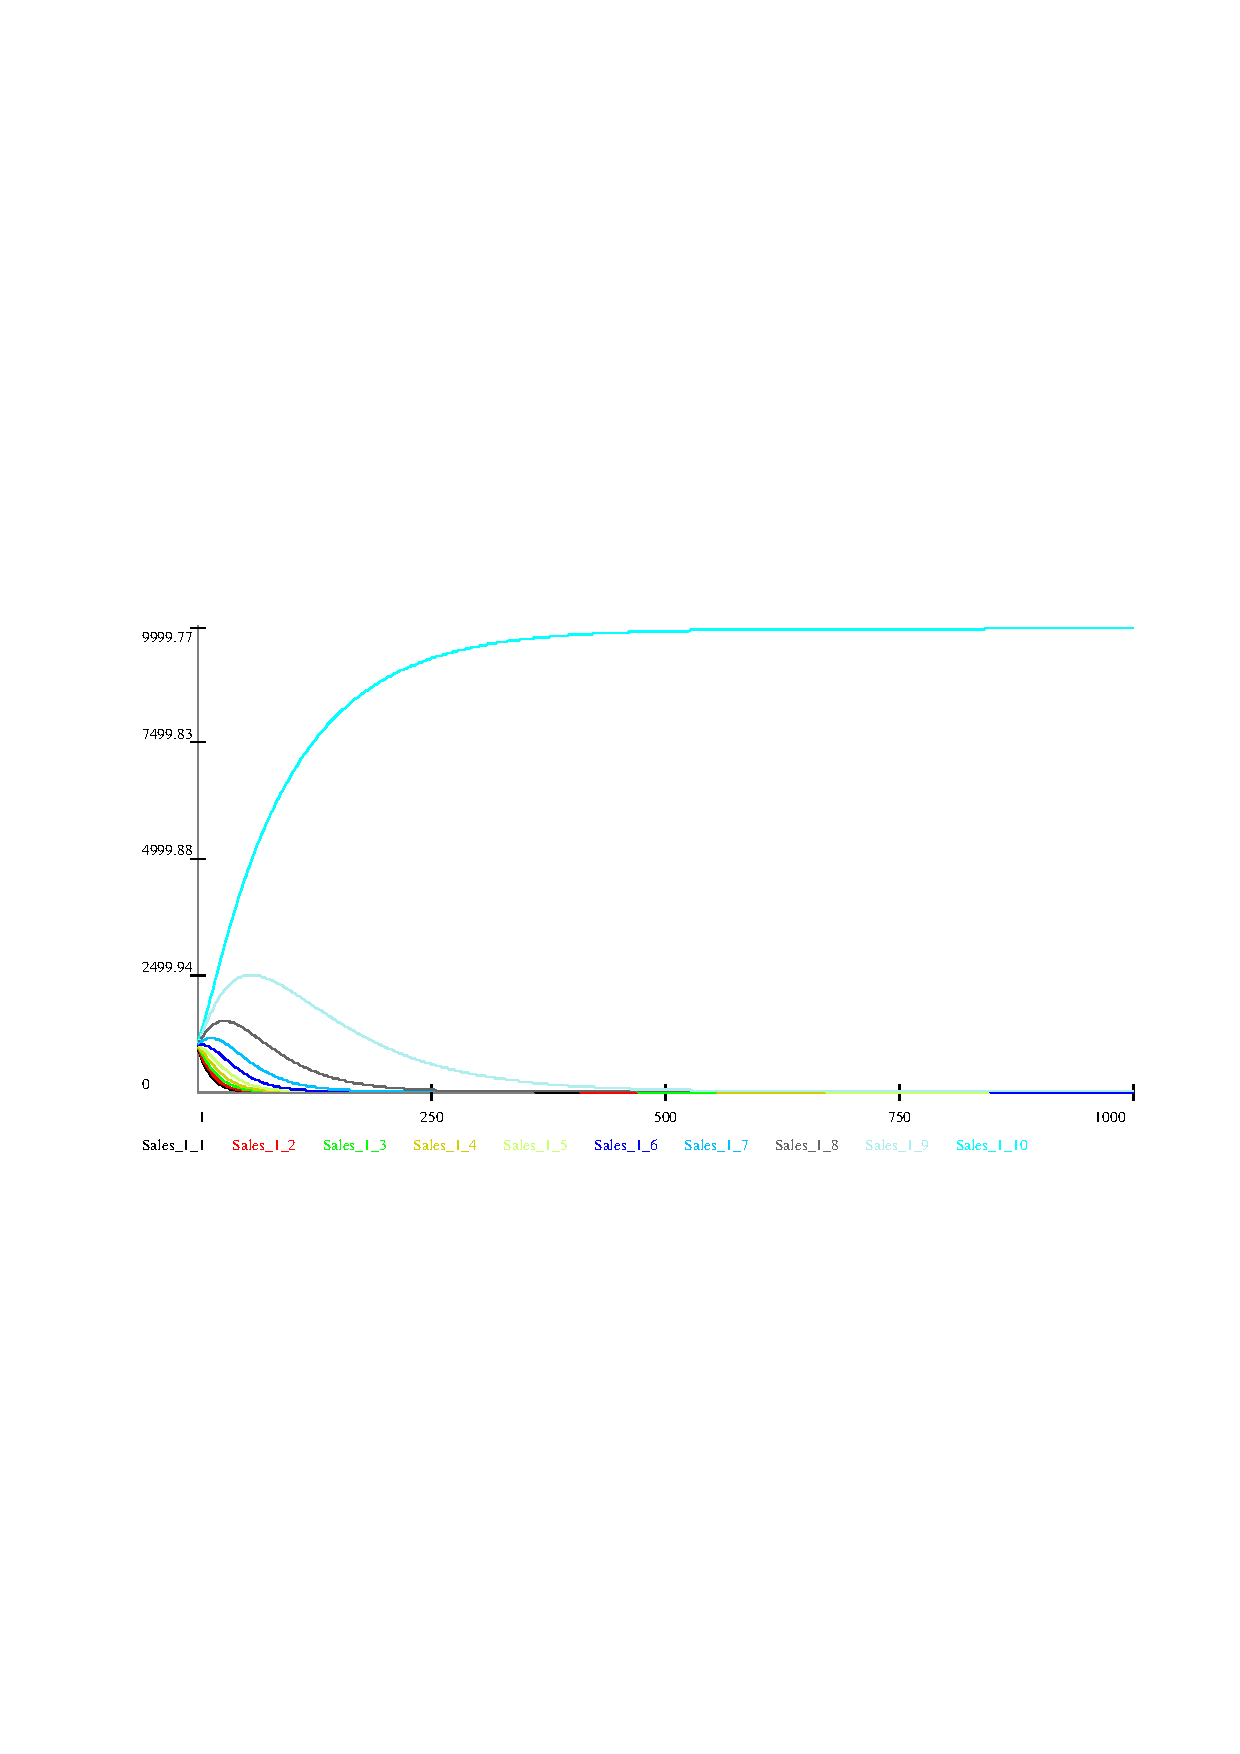
\includegraphics[height=6cm]{sales.pdf}}
  \caption{Sales time sequence with constant qualities.}
  \label{fig:sales}
\end{figure}

Now our model represents a group of firms of different, but constant, quality, and we are ready to test
how their sales levels are affected. Run the simulation, and then open the \menu{Analysis
of Results} module. Select the sales variables and plot their time sequence values. The
result should be like the graph shown in fig. \ref{fig:sales}. We can see that the
10$^{th}$ firm gains in the end all the sales, while the others decrease to 0. This is
obvious because the 10$^{th}$ firm has the highest quality. The interesting aspect of the
simulation consists in the patterns of the different sales' variables. 

Suppose you want to interpret the result according to the explanation: the dynamics of sales depend on the quality of the firms. This seems to be confirmed by the pattern of the worst firms (always decreasing) and of the very best one (always increasing). However, the second and third firm, at least, have their sales initially increasing and then decreasing: don't they have the quality constant as the others? Though the answer can easily be found logically, we can use this question as an excuse to explore another tool of \LsD: how to find detailed evidence of the micro-events within a simulation run.


\section{\LsD Debugger}
In many cases (and we may even claim the most interesting ones) we have a simulation model producing unexpected results, difficult to justify on the basis of the equations. This happen because, however simple may be the equations, the non-linear interactions among many elements through time are very hard to predict, and this is the very reason for performing simulations. Obviously, it may even be the case that our model is simply wrong, containing errors. 

In both cases it is very difficult to investigate the behaviour of the model on the basis of the time series of results alone, as they are provided by the Analysis of Results, or by a sophisticated statistical analysis. This is because reconstructing the dynamics producing the results requires a careful analysis of the events within a simulation run. For this reason you do not necessarily need a lot of data, actually too much data may be as confusing as too little. What is necessary is to access data in the appropriate way. We may even need to run a counter-factual experiment modifying what we suspect to be a crucial value. In general, we need to ``freeze'' the simulated world represented by the running model, and potentially investigate all of its elements, gaining an understanding that is much more detailed than that available looking at the resulting series alone. It is the same difference as having available the census data of a country at aggregate level along, or having the chance to reach each and every person's state: to understand how aggregate patterns emerge you need sometimes to access micro-data.


The \LsD model programs are endowed with a module that permits to interrupt a simulation
run at any moment and investigate the status of each and every element of the model, the
\LsD Debugger\footnote{The name is due to the use of this function for spotting errors,
that is bugs, in programs, when they generate unexpected results. In this case it is necessary to run the program step-by-step to reproduce and identify the sources of the error. In a simulation program, a ``bug'' may be either an error or simply an unexpected result.}.
Let's see how to use the \LsD debugger. Quit the Analysis of Results (\menu{Exit/Exit}) and re-load a fresh
configuration (press the keys \menu{Ctrl+w}).

In order to interrupt a simulation run we need to tell the model two pieces of
information: at what time step we want the interruption to occur, and, within a time
step, which equation's computation we want to observe. That is, which equation will interrupt the simulation. To ensure that no other variable is already to be debugged, use menu \menu{Run / Remove Debug Flags}.

Open menu \menu{Run/Sim.Setting} and write in the field \menu{Insert Debugger at:} a time step, say 10. After having
pressed \menu{Ok} move the \LsD Browser to show the content of \lsd{MyObj}; double-click
on \lsd{RelativeQuality} and check on the option \menu{Debug: ...} in the resulting option window
for this variable, and, finally, press \menu{Continue}. Now we can run the simulation as
usual with \menu{Run/Run}. The \LsD model program will compute the first 10 steps, and
then it will stop as soon as the first copy of a variable \lsd{Sales} complete its equation. 

Run the simulation, and the model should interrupt showing the window reported in figure
\ref{fig:debuggerSales}.


\begin{figure}[ht]
  \centering
 \fbox{\includegraphics[width=9cm]{debuggerSales.pdf}}
  \caption{Debugger set on the variable \lsd{RelativeQuality} at the 10${th}$ time step.}
  \label{fig:debuggerSales}
\end{figure}

This window provides a large number of possibilities to observe the model and, if
necessary, also to modify it in the middle of the simulation run. We will see only a few
of these now; see the menu \menu{Help/\LsD Debugger Help} for a complete
presentation for this interface. Let's see firstly the items contained in the page.

The top part of the figure, the header of the debugger, reports the label of the variable just computed when the simulation was interrupted (\lsd{RelativeQuality}), the value resulting from its computation (-0.353671), and the time step of the simulation (10).

Below the header there is a row of buttons controlling the simulation run. These
buttons operate and provide information on the dynamics of the simulation. For example,
button \menu{Run} would tell the model to continue the simulation until the end,
\menu{Quit} aborts the simulation at current time step; \menu{Step} will continue the simulation until the next variable marked to be debugged is updated. For the moment don't use any of these buttons.

The second row of buttons allows users to browse through the different copies of the
objects forming the model. For example, try to press the key ``u'' (for ``Up'') and ``d''
(for ``down'')\footnote{The underlined letters in the buttons' text indicate the keys
available as alternative to click on the buttons.}; you can also use the arrows to move around the model.

Below the buttons you find the indication on the specific copy of the model you are observing. Contrary to the \LsD browser normally used, the debugger browser does not show only the generic content of an object type, but shows the actual content of a specific copy of an object. Hence, you are shown the ordinal number of the specific copy, including the ancestors of the object up to \lsd{Root}.  Moving ``right'' across the set of \lsd{MyObj} objects you will see that their ordinal number changes.

Below the buttons you observe the how sequence of ancestors of the object currently shown (which is indicated along the label \menu{Object instance:}). Note that each element is indicated as the ordinal number of the object within its group.

The remaining part of the window shows the actual content of the object: the list of all the variables and parameters
contained in the object, indicating their current value. Note that the values of variables are tagged with a number, printed in red. This number is the time step when the variable has been lastly updated. Typically, when the debugger interrupts a simulation
run in the middle of a time step, some of the variables have already been computed, while
others still did not receive their newly computed value (e.g. variable \lsd{Sales} in the figure). Comparing the value
\menu{LastUpdate} for a variable with the current time step of the simulation shown in
the debugger's header you can see whether the variable has been already computed or not.
In our case, we interrupted the simulation when the \lsd{RelativeQuality} of the first \lsd{MyObj} has been completed. Therefore, for example, we will have that copies of \lsd{Sales} in the other \lsd{MyObj} will not be updated for the current time step, as well as all the \lsd{RelativeQuality}'s variables.


So, now we can answer our question: why some copy of \lsd{Sales} decrease while others,
non-optimal, still increase their level? Let's explore the set of objects \lsd{MyObj}. We see that all the values for \lsd{RelativeQuality} (concerning time step 9) are
negative, for the copies from 1 to 6 included. We know, from the equations, that a
negative value is caused by \lsd{RandomWalk} smaller than \lsd{WAverageRW}. Given
our set up (\lsd{minimum} and \lsd{maximum} set to 0), variables \lsd{RandomWalk} never
change. Actually, it is \lsd{WAverageRW} that does change. At time 10 this variable
has the value of 1547.2, as we can observe moving the debugger in \lsd{AggregateObj}
pressing \menu{Up}. The change is due to the changes in the weights of the average: while
higher quality firm's sales increases, so does its weight in the average, pushing up the
value of \lsd{WAverageRW}. Therefore, the values of quality for some firms was above
average in the beginning, and therefore their sales level increased. But later
\lsd{WAverageRW} increased so to overcome the levels of quality for each firm but
the 10$^{th}$, so that eventually all these firms have decreasing levels of sales.

Once a property of the model has been identified it is necessary to find the a suitable format to describe it. While the modeller has a deep knowledge of the model (and of the modeling tool), it is necessary to find a synthetic and clear format to communicate the relevant knowledge to an audience that does not have available the same tools and skills. Let's see how to prepare a clear presentation to answer this question.

Complete the simulation run, clicking on the button \menu{Run} and open the Analysis of Results. As we mentioned before we wanted to understand why sales dynamics of some firms are not monotonous, by change sign even though their qualities are constant. 

Let's consider the case of the $9^{th}$ series (the next-to-best) which increases its sales until about time step 60, and then decreases it. We can produce a graph containing its sales and quality, as well as the weighted average quality. This graph shows that the change of direction of sales for this firm takes place exactly when the firms' quality crosses the average quality.

\begin{figure}[ht]
  \centering
 \fbox{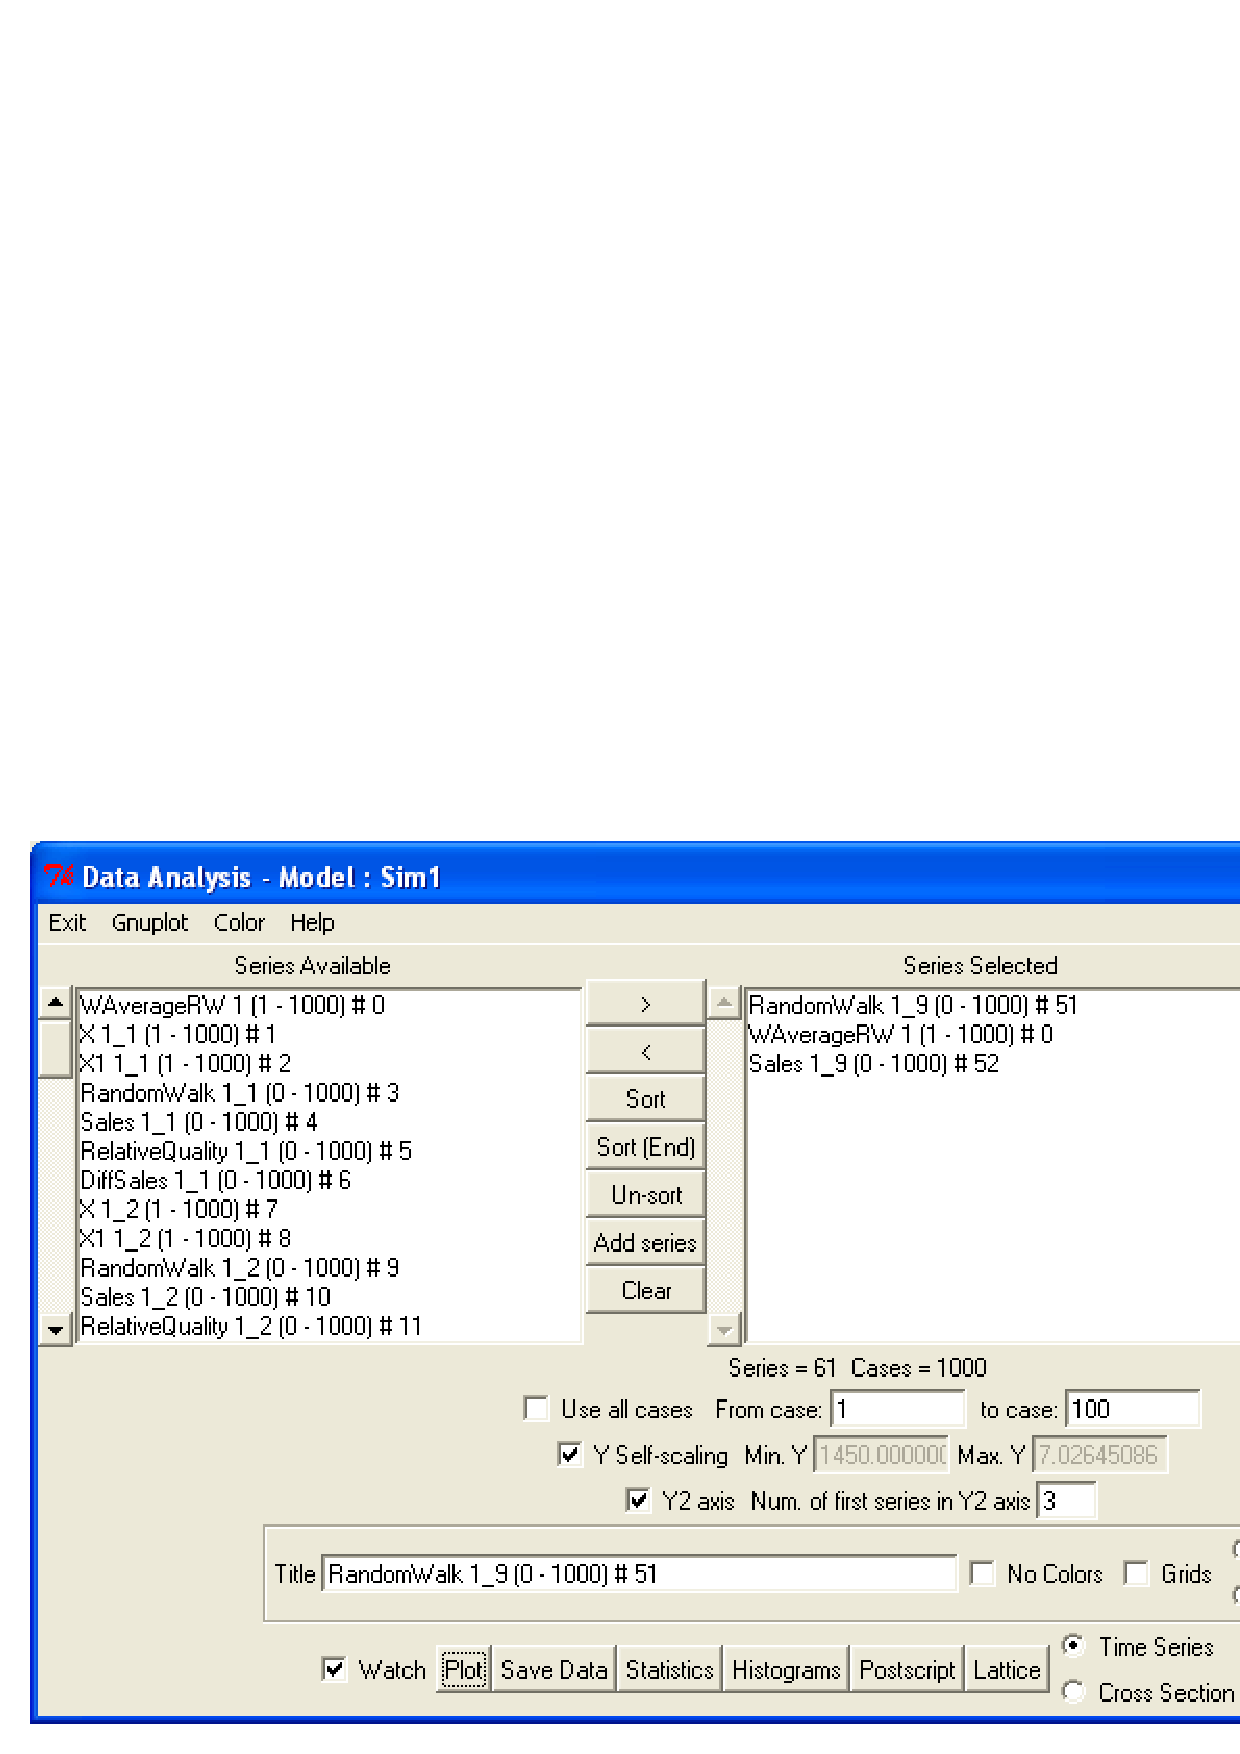
\includegraphics[width=11cm]{ansales.pdf}}
  \caption{\small Options for the Analysis of Result creating a graph using a restricted period of the simulation and using two different scales, with the second scale being used for the third series.}
   \label{fig:ansales}
\end{figure}

To generate this graph we need to make use some of the features of the Analysis of Result window. Firstly, moves in the \menu{Series Selected} box the series for the quality of the firm (\lsd{RandomWalk} with the tag 1\_9) and the average quality (\lsd{WAverageRW}). Finally, add also the sales for the same firm (\lsd{Sales}, with tag 1\_9). We need then to plot a graph restricted to the first 100 time steps, and using two different scales: one for the two qualities and one for the sales. These options can be obtained using the checkboxes and entries in the middle of the Analysis of the Result window, as indicated in figure \ref{fig:ansales}

Once the graph window has been produced we can edit it by adding, removing or editing labels. To add a label keep the shift key pressed and click on the graph window. Type into the resulting entry the text desired and confirm. To edit an existing window click on it with the right button of the mouse, and edit the text or format. To remove a label do as for editing it and assign an empty label. See the help menu for further details.


\begin{figure}[ht]
  \centering
 \fbox{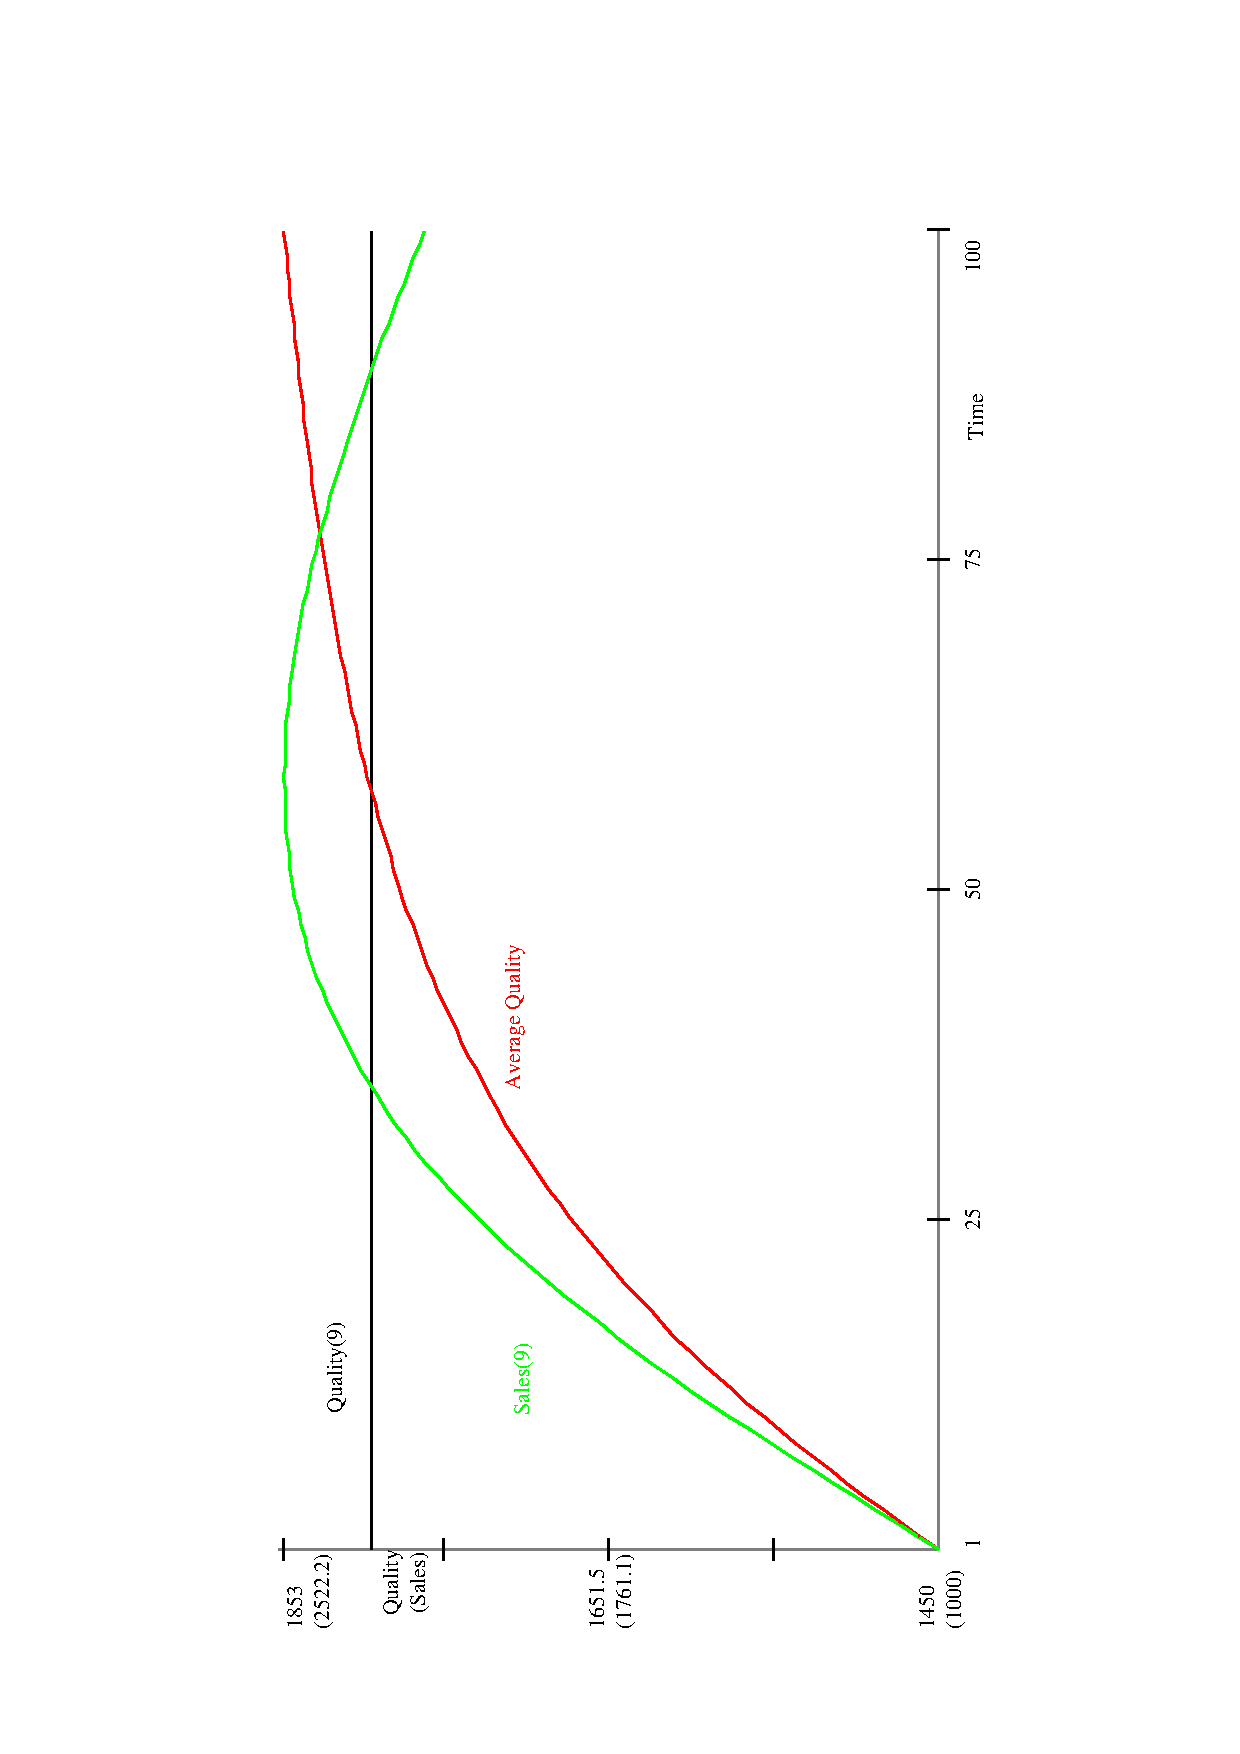
\includegraphics[angle=270,width=11cm]{RandomWalk.pdf}}
  \caption{\small Graph produced with the options as in figure \ref{fig:ansales} and edited by changing labels.}
   \label{fig:randomwalk}
\end{figure}

The resulting graph is reported in figure \ref{fig:randomwalk}. Note that the graph windows can be saved as encapsulated postscript file for use in any word-processor (again, see the help on details).

The model we developed so far is driven by the functional form we impose on the variable \lsd{Sales}. This equation represents implicitly the behaviour of the consumer, who are supposed to act in such a way to generate the prescribed dynamics of sales.

This modeling approach is generally used for mathematical models, since it can exploit convenient mathematical properties of the chosen function. But it also introduces strong rigidities on the type of models that can be generated. In our case, it is impossible, for example, modify the model to obtain a sales level positive for all firms. The model we built is, essentially, a model explaining the pattern to a monopoly, not a model of competition. For such purposes we need to devise a different model, where consumers are explicitly represented and their different preferences used to generate sales levels which are persistently differentiated, but not converging to a monopoly.

We will need to ``deepen'' the model, replacing an imposed dynamics (our equation for sales dynamics) with a derived dynamics, where sales are the result of consumers' behaviour. The resulting model will be more difficult to deal with mathematically, but will be more flexible in the type of representation. From the programming viewpoint we may continue to update the element of the model we have already generated, but it is more convenient to start a new model from the scratch to avoid confusion caused by mismatched labels or spending time re-naming many elements.

\chapter{Implementing \LsD Models: Example 2}\label{sec:tut2}

This tutorial will skip on details of the elementary operations and will focus on relatively advanced features of \LsD coding: use of functions; manual control of precedence; optimization of code. 

\section{Model Content}

The model implemented in this section is the computable version of a model originally\footnote{Smallwood and Conlisk, 1979,  ``Product Quality in Markets where Consumers are Imperfectly Informed'', \textit{Quarterly Journal of Economics}, 93-1.}implemented as a standard dynamic model, where a system of differential equations is ``solved'' providing asymptotic solutions under very strict assumptions. We will reproduce the same results by means of a computational model, which automatically allows also the possibility to observe the path leading to the limit values and provides the basis for infinite extensions.

The model addresses the issue of consumers who are not able to evaluate the quality of products they buy, neither before nor after the purchase, because of undetermined reasons. The only information available to consumer is that their product needs replacement every once in a while because it ``breaks down'', i.e. for some reason does not provide any longer its purported services. The actual quality of products, unknown to consumers, is the probability that a given product will break down at any unit of time. Consider \lsd{ProdUsed} a variable indicating which product a consumer is using. Its dynamic can be represented as follows:

$$ProdUsed_t=\left\{\begin{array}{ll}
	ProdUsed_{t-1}  & \textnormal{, if } isBroken(ProdUsed_{t-1})=0 \\
     Purchase  & \textnormal{, if } isBroken(ProdUsed_{t-1})=1 \\
\end{array}
\right.$$

where the expression $isBroken(i)$ indicates a stochastic event based on the probability that product $i$ breaks down. This may be expressed as:

$$isBroken(i)=\left\{\begin{array}{ll}
	1  & \textnormal{, with probability } BD_i \\
	0  & \textnormal{, with probability } 1-BD_i \\
\end{array}
\right.$$

where \lsd{BD\_i} indicate the quality of product $i$, hidden to consumers.

The model is completed by defining the action of consumers activated when they need to replace their broken product, defined above as \lsd{Purchase}. The model assumes that consumers rely on the only information available to them: the relative popularity of different products. The model assumes therefore that products are branded and consumers are able to recognized the brand of products, though not able to compare quality levels across different brands. Hence, they tend to choose more popular products with higher probability than those with lower market shares.

Crucially, the model assumes differences in \textit{trust} among consumers in respect of the reliability of the market shares to correlate with products' qualities. Markets where consumers have little faith that market shares are a good indicator of products' quality will tend to choose with more even probability any brand. On the contrary, markets where consumers trust market shares as a reliable indicator will concentrate their purchase only on the most popular.

The model implements this assumption by assuming that the probability of choosing any given product $i$ is the following:

$$\textnormal{Prob}(Purchase=i)= \frac{ms_i^{a}}{\sum_{j=1}^{N}ms_j^{a}}$$


\begin{figure}[ht]
  \centering
 \fbox{\includegraphics[width=10cm]{probms.pdf}}
  \caption{\small Probabilities obtained by biasing the market share of one product in respect of different values for $a$.}
   \label{fig:prob}
\end{figure}

The relation between market shares and probabilities depend on the parameter $a$. The higher $a$ the more extreme are differences between probabilities, while lower $a$ indicates flatter probabilities. Figure \ref{fig:prob} shows a visual representation of the effect of $a$. The graph reports the probability resulting for a hypothetical option among two alternatives for different values of the market share of the option and of $a$. Increasing values of $a$ clearly show the increasing polarization of probabilities. At the two extreme we have that for $a=0$ the probability is uniformly distributed irrespective of the market share. On the contrary, for high values of $a$ the product enjoying even minimal advantage obtains a probability of being chosen virtually to 100\%.

Given the two rules on the ``technology'' (when the product breaks down) and on the consumers' behaviour, the model explores the question on whether the market as a whole is able to identify the best product (least probability of breaking down), even though no single participant to the market owns such information.

In the following we are going to implement a \LsD implementation of the model able to answer this question, choosing a version able to illustrate a few advanced features of the system.


\section{Model structure and core equations}

The result produced by an equation in \LsD can (and frequently does) depend on the copy of the object containing the element. That is, the very same code of an equation associated to an element in, say, \lsd{Firm} may produce a different result if moved to \lsd{Market}. This is due to the fact that \LsD fills automatically many details left un-specified in the code by inducing the intention of the modeler from the position of the variable in the model structure. Relying on automatic rules not only requires far simpler code from modelers, but it is also central in the possibility of modifying existing models and re-using code in different models, since the system automatically re-arrange the code to changing conditions.

Because of the importance of the model object structure, let's start by defining the objects into which we will place our computational content. The structure is pretty straightforward: we define an object \lsd{Market} containing a \lsd{Supply} and \lsd{Demand} side. In turn, \lsd{Supply} contains several objects \lsd{Firm} and \lsd{Demand} several objects \lsd{Consumer}. The structure of the model is reported in figure \ref{fig:abm}.

\begin{figure}[ht]
  \centering
 \fbox{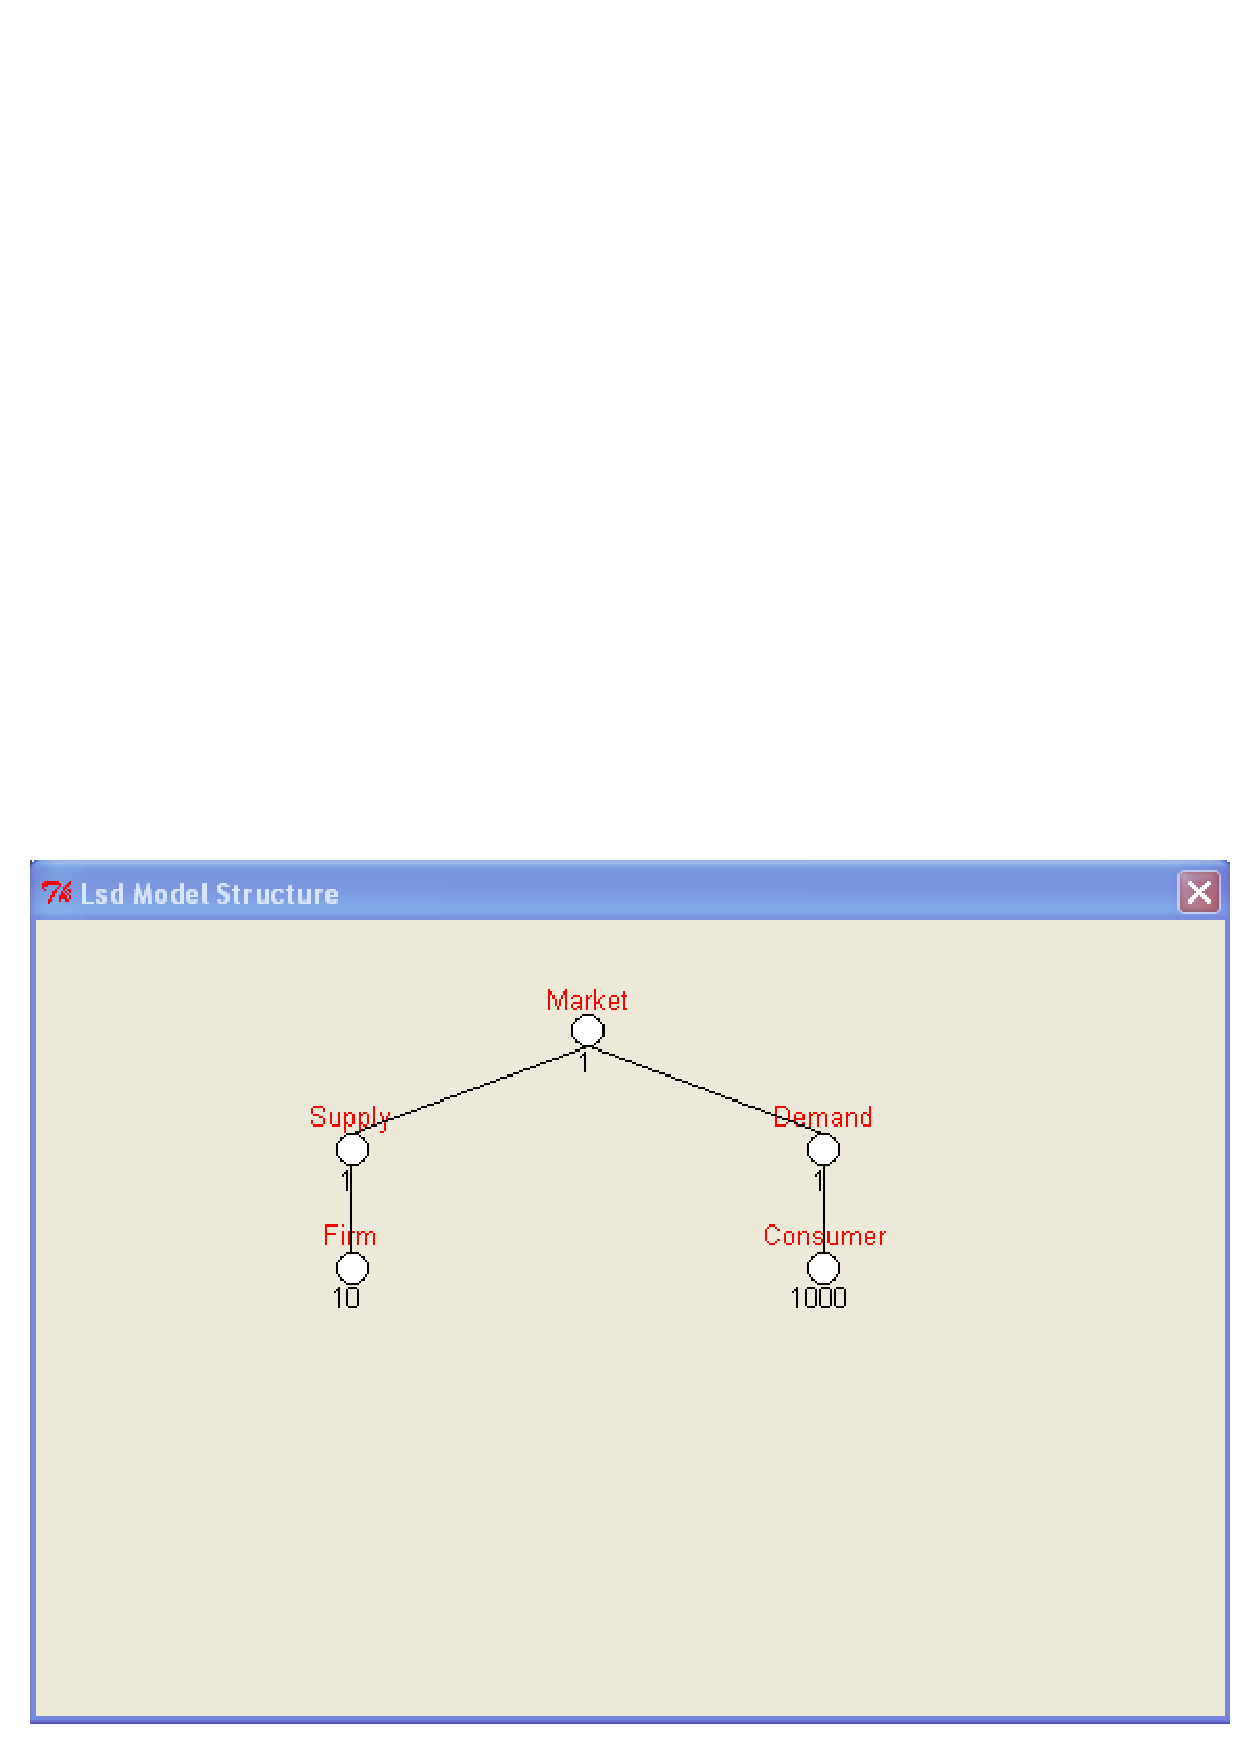
\includegraphics[width=8cm]{abmobj.pdf}}
  \caption{\small Object structure of an model. Object \lsd{Market} contains \lsd{Supply} and \lsd{Demand}, which, respectively, contain \lsd{Firm} and \lsd{Consumer}.}
   \label{fig:abm}
\end{figure}


Let's define a ``brand'' for each firm, that is a way to identify a product from others. To do so we can simply define a parameter in the objects \lsd{Firm} initialize with a different value (say 1, 2, etc.) for each copy. Insert parameter \lsd{idFirm} in the object \lsd{Firm} and assign as initial values increasing integers starting from 1 (use \menu{Set All} and option \menu{Increasing}, using 1 as starting point and 1 as step). Also, assign to the same objects the ``quality'' of products to each firm, that is the parameter indicating the probability of breaking down for users of each firm's products. Insert parameter \lsd{BD} and assign 0.1 to the first firm, and then increase the value by 0.01 to each following firms (as beforem \code{Set All} and \menu{Increasing}, using starting value 0.1 and increasing by step 0.01).


Let's start by writing the code for the equation concerning the product used by consumers. The variable will indicate at time $t$ the id of the product used by the consumer. Its equation can be expressed as follows

\begin{verbatim}
EQUATION("ProdUsed")
/*
Determine the product used by the consumer
*/
v[0]=V("IsBroken"); //breaks ?
if(v[0]==1)
  v[1]=V("Purchase"); //yes, buy a new product
else
  v[1]=VL("ProdUsed",1); //no, keep on using the previous one
RESULT(v[1])
\end{verbatim}

The code is pretty straightforward, but a few comments may be useful. Firstly, we avoided tackling the main problem by delegating element \lsd{IsBroken} to produce the crucial information on whether the product breaks down. Once this is resolved, the equation is a mere conditional statement. Note that the logical condition ``is equal'' is expressed with the double equal sign \code{==} in C++. If the condition is true the first line is executed and the \textit{else} command is skipped, and the opposite in case the condition is not verified.

Similarly, if a new product must be chosen the equation relies on another element of the model to make the necessary operation, \lsd{Purchase}, which will have to return the \lsd{idFirm} of a newly purchased product. Alternatively, if the product is not broken, the variable \lsd{ProdUser} will continue to have the value as at the previous time step.

\section{Finding model data in \LsD equations (equation for \lsd{IsBroken})}

Let's see the code for the variable \lsd{IsBroken} whose main problem concerns the possibility to access the appropriate data from the model. We start by writing an intuitive, but wrong, version for the equation, and then, fixing the errors, we will eventually reach a correct version. The incremental versions of the model will provide the excuse to discuss the different ways modeler can control the data used by equations for their computation, that is, which copy if a given element, among many, is used within the code for an equation. The system provides, by default, a certain copy depending on the location of the element associated to the equation. However, the user can overrule the default system.

The computational content of the equation for \lsd{IsBroken} is not very complex. The difficult part concerns the access to the necessary data. Consider the following formulation:

\small
\begin{verbatim}
EQUATION("IsBroken")
/*
Check if the product is broken. INCREMENTAL VERSION 1.0
*/
v[2]=V("BD"); //should be the b.down probability
if(RND<v[2])
  v[1]=1; //product broken
else
  v[1]=0; //product not broken
}
RESULT(v[1] )
\end{verbatim}

Provided that the local variable \code{v[2]} contains the probability of breaking down, the code is pretty trivial. The conditional statement \code{if(...)} emulates a random event. The \LsD function \code{RND} produces a random value uniformly distributed in [0,1] every time it is executed. Hence, for example, if \code{v[2]=0.1}, the condition \code{RND<v[2]} will be true or false 10\% and 90\% of times  it is executed, respectively. In the first case it returns 1, and in the second 0, providing the required result for the equation of \lsd{ProdUsed}. 

\subsection{Automatic data retrieving}

The code for the equation, however simple, cannot produce the result we expect because the system is not able to produce the correct value of \lsd{BD} in the equation. In fact, without any specifier (i.e. using only \code{V(...)}), the system decides on its own where to retrieve elements requested during a simulation run. Consider the structure of object we built for our model (figure \ref{fig:abm}); whatever object you decide to place variable \lsd{IsBroken} in, the result will not be the one desired. 

To understand why, we need to consider how \LsD retrieves automatically the data within the equations. Consider the equation for a variable, say \lsd{Y}. When the code encounters a command requiring data from the model, e.g. \code{V("X")}, it starts searching an element of the model with label \lsd{X} in the same copy object containing the copy of variable \lsd{Y} under computation. This object is referred to by a pointer, \code{p}, that, contrary to \code{cur}, cannot be assigned by modelers but it is set by the system for each equation. If the object contains the element, i.e. if the object containing \lsd{Y} contains also \lsd{X}, the system returns the value from this copy. Alternatively, if the object containing \lsd{Y} does not contain element \lsd{X}, the system starts a search scanning potentially all objects in the model, according to a precise order. Below is the strategy adopted to automatically search elements necessary for an equation.

\begin{enumerate}
\item Search in the object \code{p}.
\item Search in all objects descending from \code{p}.
\item Search in the object containing \code{p}.
\end{enumerate}
 
 The search routine is recursive, that is, replicates the same strategy in every object visited, with the obvious control that it does never pass twice in the the same object. The first object found during the search containing \lsd{X} the search stops and the value of the element is returned.

\subsection{Manual data retrieving}
Considering that parameters \lsd{BD} are contained in objects \lsd{Firm}, and given the search routine, wherever you placed \lsd{IsBroken} the result of the equation as written above will be wrong, that is, it will not produce the intended result. The problem is that the copy of parameter \lsd{BD} to be used cannot be automatically delivered by the automatic system, but needs to be the one indicated by the content of the past value of \lsd{ProdUsed} of the object consumer using this code. In other word, the same code for \lsd{IsBroken} used by the same copy of object consumer will need to deliver a different copy of \lsd{BD}; this means that the code needs to specify ``manually'' how to retrieve that copy.

The following equation shows how the modeler can by-pass the \LsD automatic retrieval system and find a value for a specified copy of an element, in our case a specific firm.

\small
\begin{verbatim}
EQUATION("IsBroken")
/*
Check if the product is broken. INCREMENTAL VERSION 2.0
*/
v[0]=VL("ProdUsed",1);
cur=SEARCH_CND("idFirm",v[0]);
v[2]=VS(cur, "BD");
if(RND<v[2])
  v[1]=1; //product broken
else
  v[1]=0; //product not broken
RESULT(v[1] )
\end{verbatim}

Let's see firstly the new command introduced in this code. The first line of the equation loads in \code{v[0]} the unique identifier of the product owned by the consumer in the previous time step, \lsd{ProdUsed} with one lag. Notice that \lsd{IsBroken} is computed during the computation of \lsd{ProdUsed}, thus any line in the equation such as \code{v[0]=V("ProdUsed");} would cause a dead-lock error; but here we are asking for the \textit{past} value of a variable under computation, and this value can be obtained without triggering the computation of the equation.

The second line contains the new command, \code{SEARCH\_CND("Label",val)}. In general, this command implements a search for the element called \lsd{Label} following a search strategy identical to the one discussed before for the automatic retrieval system. However, the search does not stop as soon as on copy of the element is found, but continues until the copy of the element has a value exactly equal to \lsd{val}. If the system does not contain any element \lsd{Label} with value \code{val}, then the simulation stops issuing an error. Conversely, if one such an element is found, the command returns the object containing this element. 

Besides the new command, the code of the equation is straightforward. The local pointer \code{cur} will contains the copy of \lsd{Firm} whose parameter \lsd{idFirm} equals the past value of \lsd{ProdUsed} of the consumer. The copy of the \lsd{BD} parameter will be the one contained by the selected \lsd{Firm}, and hence the random event will be computed as before.

\subsection{Functions vs. Variables}
This implementation 2.0 of the equation works provided a crucial condition is respected. The condition is that the line \code{v[0]=VL("ProdUsed",1);} is able to return the (past) value from the copy of the variable of the consumer we are computing. To ensure this we need to locate \lsd{IsBroken} within the same object as \lsd{ProdUser}, i.e. in object \lsd{Consumer}. This choice is not, however, particularly elegant. We likely wish to have a large number of consumers, and the least number of elements we place there the smaller will be the memory requirements. Besides, the simulation needs not to store the information produced by \lsd{IsBroken}, since we are only interested in which product a consumer is using. Hence, we may consider to place the element \lsd{IsBroken} somewhere else, for example in object \lsd{Supply}, so that every consumer may exploit its code, but not own an individual copy. This choice, computationally more efficient, generates however two problems.

The first problem derives from the choice of having a single element \lsd{IsBroken} and many variables \lsd{ProdUsed} asking its value. This implies that the equation for \lsd{IsBroken} needs to be re-computed several times at each time step. In fact, suppose that the first consumer uses \lsd{IsBroken}, adopting the probability of breaking down of its currently owned product. At the same time step, the second consumer will need to re-compute the same code. But \LsD prevents variables to re-execute the code for their equation twice in the same time step. Hence, the result provided by the first use of \lsd{IsBroken} will be passed to all consumers, causing the wrong result that all consumers will have their product broken, or not broken, at every time step. To avoid this result we need to define \lsd{IsBroken} not as a \LsD variable, but as a function. In \LsD functions are not constrained to be computed only once at every time step and to return the same value without recomputing the equation every time they are asked so in the same time step. On the contrary, functions have their equation re-computed again and again an element  of the model (that is, an equation) requires their value, which is exactly what we need here. Nota that it is possible also to ask for \textit{lagged} value of a function, such as, e.g., in \code{v[0]=VL("IsBroken",1);}, though the meaning is different in respect of lagged variables. When asked for lagged values of functions the system does not compute their equation, but returns the value computed at the latest execution of the equations' code, independently from the time step in which it had been computed.

\subsection{Accessing the \texttt{c}alling object}
 
The second problem is that placing the element \lsd{IsBroken} in an object different from consumers, we cannot ensure that the very first line works properly. In fact, if the function is located in \lsd{Supply}, or anywhere else but consumer, the copy of \lsd{ProdUsed} in the first line is not determined, and the automatic data retrieving is almost certain to fail to produce the correct value. We need to ensure that the copy of the \lsd{ProdUsed} used in \lsd{IsBroken} comes from the same copy of consumer that is forcing the computation. This result is not possible by relying on the automatic data retrieval, because this will always return the first copy found. Nor it is possible to use \code{SEARCH\_CND()} because we do not have an identifier for consumers. So, we need to use a third mechanism available to identify a specific element among many copies.

\small
\begin{verbatim}
EQUATION("IsBroken")
/*
Check if the product is broken. INCREMENTAL VERSION 3.0
*/
v[0]=VLS(c,"ProdUsed",1);
cur=SEARCH_CND("idFirm",v[0]);
v[2]=VS(cur, "BD");
if(RND<v[2])
  v[1]=1; //product broken
else
  v[1]=0; //product not broken
RESULT(v[1] )
\end{verbatim}

The difference with the previous version is that the first line does not ask a generic copy of \lsd{ProdUsed}; rather it specifies where the element must be searched in. Note the grammar of the usual command \code{V()}, which in this case it becomes \code{VLS(...)}  combining both the modifier for lags as in \code{VL(...)} and for specific objects \code{VS(...)}. The implementation uses the pointer \code{c}, which is a system-set pointer (as for \code{p}), indicating the object of the element whose equation requested the current equation to be computed (the name derives for the \underline{\code{c}}alling object). In our case, the variables \lsd{ProdUsed} trigger the computation for \lsd{IsBroken}, so any time the equation is computed, the pointer \code{c} will indicate the consumer containing \lsd{ProdUsed} whose equation caused the computation of \lsd{IsBroken}. Using the system-set object \code{c} is almost always restricted to functions, because they are always executed on request by other equations, and therefore there is always an object calling their equations. On the contrary, variables may be computed also because of the mere need to update their value, not because requested by other equations. In this case the pointer \code{c} is not set, and its use in the equation will cause an error. 

\subsection{Accessing a randomly chosen object}

We know that consumers choose a novel product (when they need to buy one) with probabilities proportional to the normalized value of the formula $ms^{a}$. So, we need to produce the equation for this variable, that we may call \lsd{Visibility}.

\small
\begin{verbatim}
EQUATION("Visibility")
/*
Visibility of the firm used by consumers
when purchasing a product
*/

v[0]=VL("ms",1);
v[1]=V("a");
v[2]=pow(v[0],v[1]);
RESULT(v[2] )
\end{verbatim}

The only remarkable aspect of this equation is that you need to use \textit{past} market shares, because this variable is used by consumers to make decisions that collectively will allow to compute present-time market shares. Using the value of $ms_t$ to compute a variable necessary to compute itself will obviously produce a dead-lock. Also, note the grammar for the power function, which one of the mathematical expressions available in C++ and inherited in \LsD.

The equation for \lsd{Purchase} uses this value to pick a randomly chosen firm and return its \lsd{idFirm}. The logical operations for random choices are rather complex: compute the number of alternatives; assign probabilities; draw a random value; etc. However, it is so frequently used that \LsD provides a single line command performing all necessary operations on the basis of the the information provided by the modeler. Thus, the code for \lsd{Purchase} is very small.

\small
\begin{verbatim}
EQUATION("Purchase")
/*
INCREMENTAL VERSION 1.0
Make a purchase for the calling object (supposedly a consumer).
RNDDRAW("Obj", "Label") is a Lsd function choosing randomly an
object called "Obj" probability equal to "Label".
*/
cur=RNDDRAW("Firm","Visibility");
v[0]=VS(cur,"IdFirm");
RESULT(v[0] )
\end{verbatim}

The \LsD command \code{RNDDRW("Obj", "Label")} can be used only in the equations for elements contained in objects up in the hierarchy that contain as descendants the group of objects to choose, \code{Obj}. The element \code{Label} refers to the elements whose (normalized) values must be used as probabilities. The command returns the pointer to the chosen object which, in our case, provides the id of the firm to be used as result of the equation. Note that the command \code{RNDDRW()} automatically normalizes the values used as probabilities so that, as in our case, the sum of \lsd{Visibility}'s is not, in general, 1.

\lsd{Purchase} needs to be located in an object containing the firms, so will be located in \lsd{Supply}. Moreover, the code of purchase serves all consumers, and needs to be re-computed every time a consumer needs to make a purchase. Hence, this must be defined as a function, not a variable, otherwise once chosen a product $i$ for one consumer, all other consumers will choose the same product in that time step.


\section{Using parameters as ``passive'' variables}

We have seen that the model needs to compute the market shares of different firms. The equation for market share is pretty trivial:

\small
\begin{verbatim}
EQUATION("ms")
/*
Market shares of a firm, computed as number of consumers 
using the product (NumUsers) divided by total number 
of consumers (TotUsers)
*/
v[0]=V("NumUsers");
v[1]=V("TotUsers");
RESULT(v[0]/v[1] )
\end{verbatim}

Obviously, we expect that the variable \lsd{ms} will be located in objects \lsd{Firm} together with \lsd{NumUsers}, indicating the current customer base of the firm. Variable \lsd{TotUsers} will instead be located in an aggregate object, such as \lsd{Supply}\footnote{The code for \lsd{TotUsers} is not reported, assuming the reader is able to implement the code for the sum of \lsd{NumUsers}.}.

The equation for \lsd{NumUsers} will be expressed as the net variation of previous period value after summing newly acquired customers and subtracting lost ones, i.e. customers owning the product of the firm but discovered it has broken in the current time step.

\small
\begin{verbatim}
EQUATION("NumUsers")
/*
Number of consumers using this product
Computed as NumUsers[t-1]+Sales[t]-Lost[t]
*/
v[0]=VL("NumUsers",1);
v[1]=V("Sales");
v[2]=V("Lost");
RESULT(v[0]+v[1]-v[2] )
\end{verbatim}

While their meaning is trivial variables \lsd{Sales} and \lsd{Lost} pose a serious problem: how can we compute them?

In \LsD variables express the changing values according to a computational algorithm, i.e. they represent an ``activity'' of the object in which they are located. But in the case of these variables we do not want to express any active computation by firm; on the contrary, they are sort of passive accounting book in which the model actors (the consumers) will write the result of their actions. In \LsD it is possible to use variables without a specific equation, that rely on other equations to change their value. Actually, though they are conceptually variables in the model because they change value through time, they are technically implemented as \LsD parameters, because they lack an equation. So, add the two parameters \lsd{Sales} and \lsd{Lost} in object \lsd{Firm} and then we need to refine previous equations to ensure that the information required to have \lsd{Sales} and \lsd{Lost} correctly computed in inserted.

Consider, first, the case for \lsd{Lost}. This variable needs to express the number of customers of a given firm whose product broke down. Interpreting the variable as an action by the firm, this would need to write the code to scan each and every consumer controlling whether its product broke down. This is obviously highly inefficient, because we would need to scan all consumers for each firm. Besides, we already know whether a consumer has its current product broken, and therefore we can piggyback on the code for \lsd{IsBroken} to play two distinct roles in the model: to consumer provides the information of breaking product, and to the firm provides the information on a consumer lost.

Consider this fourth version for \lsd{IsBroken}:

\small
\begin{verbatim}
EQUATION("IsBroken")
/*
Check if the product is broken. INCREMENTAL VERSION 4.0
*/
v[0]=VLS(c,"ProdUsed",1);
cur=SEARCH_CND("idFirm",v[0]);
v[2]=VS(cur, "BD");
if(RND<v[2])
 {
  v[1]=1; //product broken
  INCRS(cur,"Lost",1);
 } 
else
  v[1]=0; //product not broken
RESULT(v[1] )
\end{verbatim}

The additional code contains the command \code{INCR("Label",val)} that modifies the content of an element in the model. As for most of the \LsD commands there are several variations of the command grammar; in our case we use the \code{INCRS(pointer, ...)} version that allows to specify a given object where it should be applied, as in \code{VS(...)}.

The command is among among a few that changes the value of the element indicated by \code{Label}. The command increases the value of the element by adding the value \code{val} to the previous value. In short, the amended code not only provides the consumer with the information on whether its product broke down, but also tells the firm that it had lost a customer, updating the counter of the consumers who had the same experience.

We can use the same system for \lsd{Sales}. Since \lsd{Purchase} already gets the firm chosen by a consumer, we may use this code to update the (passive) variable. 

\small
\begin{verbatim}
EQUATION("Purchase")
/*
INCREMENTAL VERSION 2.0
Make a purchase for the calling object (supposedly a consumer).
RNDDRAW("Obj", "Label") is a Lsd function choosing randomly an
object called "Obj" probability equal to "Label".
*/
cur=RNDDRAW("Firm","Visibility");
INCRS(cur,"Sales",1);
v[0]=VS(cur,"idFirm");
RESULT(v[0] )
\end{verbatim}


\section{Manual scheduling: semaphores}

Whenever the value of one variable, say $X_t$, is used in one equation the modeler generally does not need to ensure that the variable is already updated. The system ensures that $X$ have executed its own equation to get updated before using its value in another equation.  However, this system cannot work for passive variables, such as \lsd{Sales} and \lsd{Lost}. The system considers them as parameters, and does not attach any time tag to their values, being constant or changing. It is the modeler then that needs to ensure that the simulation cycle is such as to schedule all the operations involving these elements in the correct order.

If we ran the model as it is coded now the result would be disastrous. Suppose, for example, that you initialize \lsd{Sales} to 0. At the first time step all firms get their copy of \lsd{Sales} reflecting the number of customers who bought their product. For example, assume one firm gets its \lsd{Sales} equal to 100. Consider the content of \lsd{Sales} at the end of second time step. These parameters have been increased by the sales in the first step, and again increased by those in the second. Hence, \lsd{Sales} and \lsd{Lost} represent not the values at each time step, but the \textit{cumulated} values, which is clearly not what we want to implement.

This is due to the passivity of these elements, reflected in their nature as \LsD parameters. The system does not have the means to control when the parameter is modified by the equations of the model, hence it is up to the modeler to manually construct a computational schedule ensuring that the desired values are correctly computed.

If we want that \lsd{Sales} and \lsd{Lost} reflect the behavior of consumers at a single time step only, and not the cumulated values from previous periods, we need to ensure that the very first operation at the beginning of a time step consists in resetting to 0 the values of \lsd{Sales} and \lsd{Lost}.  This is done by the following equation.

\small
\begin{verbatim}
EQUATION("InitTrade")
/*
Ensures that Sales and Lost
are set to 0
*/
CYCLE(cur, "Firm")
 {
  WRITES(cur,"Sales",0);
  WRITES(cur,"Lost",0);
 }
RESULT(1 )
\end{verbatim}

The code contains a member of the command \code{WRITE("Label",val)} which search in the same object as the computed variable the element \code{label} and replace its value with \code{val}. The version used in the code (\code{WRITES(...)}) searches the element in the object specified by the pointer in the first field.

The element \lsd{InitTrade} is of no interest as far as the results of the model are concerned, as reflected by the fact that the result value is a constant (may be any value but it is necessary to specify a number, 1 in the example). The equation is purely a service element that only prepares the stage for the passive variables to get properly computed.

In general \LsD modelers do not need to worry on the precedence of computations, that is, the schedule of the equations of the model because the system is able to use the variables time tags to arrange a coherent order of computation, if it exists (or issue a deadlock error message). But this is not the case when we use passive variables. The system may execute the equation for \lsd{InitTrade} \textit{after} consumers made their decisions, therefore preventing firms to read the values they need. So, we need to tell the model that \lsd{InitTrade} needs to be computed before any other equation. There are two alternative systems to obtain this result.

Firstly, modelers can exploit the way \LsD produces its own automatic schedule of operations, i.e. how it design one of the possible order of execution of the model equations. The general rule is that \LsD starts trying to update the elements in the top objects of the hierarchy: first \lsd{Root}, then its descendants, and so on. Hence, placing \lsd{InitTrade} high in the hierarchy we have a high probability that its equation is computed before anything else. But this solution dangerous. If the very first equation executed at the beginning of a time step requires an updated value from another variable, the system turns to compute the latter before completing the former. Hence, even if we painstakingly control that this does cause disruption in our model, we still leave the possibility that any future change to the code will overlook the need for \lsd{InitTrade} to be computed early on in the schedule. So, if you produce an extended version of the model, or one user wants to re-use the code, the priority is no longer ensured. These types of errors are particularly nasty because the system does not issue any error: simply the results are different from what one expects.

The second solution is, contrary to the former, highly reliable and robust to changes of the model. It consists in exploiting the automatic scheduling system by explicitly preventing the wrong precedences to occur. That is, we can tell the system that it can proceed with a certain operation only after another one has been completed. In our case we need to we can obtain this result by editing the equation for consumers as follows:

\small
\begin{verbatim}
EQUATION("ProdUsed")
/*
Determine the product used by the consumer
*/
V("InitTrade"); //the semaphore
v[0]=V("IsBroken"); //breaks ?
if(v[0]==1)
  v[1]=V("Purchase"); //yes, buy a new product
else
  v[1]=VL("ProdUsed",1); //no, keep on using the previous one
RESULT(v[1])
\end{verbatim}

The code is identical to the former version but for the very first line. It asks the (useless) value of the variable \lsd{InitTrade}. Obviously, it is not its value we are interested into (which is not even assigned to any local variable). We just want to ensure that the system proceed to the following lines only after \lsd{InitTrade} is computed. If the copy of \lsd{ProdUsed} is executed when \lsd{InitTrade} have not been updated at the present time step, then the necessity to compute its value triggers its equation. Since it is a variable, any subsequent call for its value will not trigger another computation, but the previously computed (useless) value will be returned. In essence, \lsd{InitTrade} acts as a \textit{semaphore}, stopping the traffic of computation until a given equation completes its own.

Our model needs a second semaphore, again because of the presence of passive variables in the model. While \lsd{InitTrade} ensures that the cumulation of data starts at each time $t$ from 0, without carrying erroneously data from the past time step, we need similarly to ensure that we use the computed values for \lsd{Sales} and \lsd{Lost} only when their values are correctly computed. In fact, we use \lsd{Sales} in the equation for \lsd{NumUsers}, and we need to avoid that a firm uses the passive variables before all consumers have made their choices. So, we build a second semaphore, call it \lsd{EndTrade}, and place it in the equation for \lsd{NumUsers}.

\small
\begin{verbatim}
EQUATION("EndTrade")
/*
Semaphore signaling the end of 
consumers activity
*/
CYCLE(cur, "Consumer")
  VS(cur,"ProdUsed");
RESULT(1 )
\end{verbatim}

This variable, located in \lsd{Demand}, appears as updated to the system only if all consumers completed their choice. Hence, we can edit the equation for \lsd{NumUsers} as follows in order to ensure that the levels of \lsd{Sales} and \lsd{Lost} for the firm reflect the decisions of all consumers.


\small
\begin{verbatim}
EQUATION("NumUsers")
/*
Number of consumers using this product
Computed as NumUsers[t-1]+Sales[t]-Lost[t]
*/
V("EndTrade");
v[0]=VL("NumUsers",1);
v[1]=V("Sales");
v[2]=V("Lost");
RESULT(v[0]+v[1]-v[2] )
\end{verbatim}


\section{Initialization by code}

Any  \LsD model program is automatically endowed with interfaces allowing rather sophisticated initializations, i.e. assigning number of objects and initial values to parameters and lagged variables. However, there are some aspects of models that are difficult, time-consuming and error prone the initialize properly. In these cases it may be fare easier to write the code of an initialization routine assigning values to the model element at the very start of a simulation run.

In our model we could run the model as it has been defined so far, but the initialization would be relatively annoying. For example, and primarily, we need to ensure that the value of parameter \lsd{TotUsers} is identical to the number of copies of objects \lsd{Consumers}, meaning that every time we change one we need to remember to also change the other. 

There are also other constraints we need to respect in the initialization. The reason is that the model is designed to maintain a rigid coherence between data from different objects, namely consumers' and firms' data. That is, the values in \lsd{NumUsers} need to correspond to an equal values of \lsd{ProdUsers} showing the identification of the firms. So, for example, if the firm with \lsd{idFirm}=3 has the value of \lsd{NumUsers}=154, you need to ensure that in your model there are 154 consumers whose variable \lsd{ProdUsers}=3. The model ensures that a coherent configuration is maintained through time, but at the very beginning it is the initialization that needs to ensure we have a coherent condition to start from.

The manual initialization using the \LsD interfaces is feasible but not practical, unless to force very peculiar conditions (e.g. all consumers start using the same product, which will start with 100\% of market shares). Thus, we better write the code for an equation whose variable exist only at the beginning of a simulation run and is then removed. As we will see the time necessary to write the code for a generic equation is a fraction than those required for a single coherent configuration by manual initialization.


\small
\begin{verbatim}
EQUATION("Init")
/*
Initialize the model coherently
*/
V("InitTrade");
v[0]=V("TotUsers");
cur=SEARCH("Demand");
ADDNOBJS(cur,"Consumer",v[0]-1);
CYCLE( cur, "Consumer")
 {
  v[1]=V("Purchase");
  WRITELS(cur,"ProdUsed",v[1], t);  
 }
PARAMETER
RESULT(1 )
\end{verbatim}

The equation implements the code for a \LsD variable located in \lsd{Root}. We already mentioned that it is good practice not to use this object to contain elements because of the specificity of this object. However, for the same reason \lsd{Root} is particularly convenient to store an initialization routine. The object \lsd{Root} is the only one in a model that cannot be replicated in many copies. Moreover, the automatic update of variables start always from \lsd{Root}, hence the first variable in this object will certainly be executed before anything else.

Let's see the code for the equation. The first line fires the semaphore so that, at the very first time step, it is not re-computed again. At time \code{t=1} in fact the semaphore is useless, since the values of \lsd{Sales} and \lsd{Lost} will be empty because there were ne previous computations loading into them past values.

The second line reads the number of consumers in the model as expressed in \lsd{TotUsers}. The following command (whose grammar is obvious) searches the object \lsd{Demand} and stores it in the pointer \code{cur} . Then the code shows an advanced command; the line generates a number (exactly \lsd{TotUsers}-1) of new copies of objects \lsd{Consumer}, and place them into \lsd{Demand}. This line obviously assumes that the model configuration is defined as containing a single copy of object \lsd{Consumer}. 

The subsequent cycle scans all consumers in the model and, for each of them, imposes a new value for \lsd{ProdUsed}. Note that the command \code{WRITELS(cur,"ProdUsed",v[1], t);)} is used in a peculiar version. Firstly, it needs to specify the object containing the copy of \lsd{ProdUsed} it needs to write onto at that round of the cycle, hence, following the usual convention in \LsD it has the modifier \code{-S}.  Secondly, it also uses the modifier \code{-L} normally used to mean lagged values. In this case, however, this indicate the time at which the variable concerned by the command must appeared as being computed. The last field of this command indicates that all the variables \lsd{ProdUsed} for consumers will show as time tag the value contained in the system variable \code{t}, which is a variable controlled by \LsD indicating the current time step of the simulation run. In our case we may replace \code{t} with 1, since we know that this equation will be computed only in the first time step and never again.

To ensure that the equation is computed only once, the last line of the equation contains a command that affects the very element whose equation is computed. The command \code{PARAMETER} orders to the element using the equation (which, having an equation must necessarily be either a variable or a function) to turn itself into a parameter. By doing so, the model ensures that the same code will never be repeated again in the time step following the first. In the rest of the simulation, the system passing through \lsd{Root} will find not variable \lsd{Init}, but \textit{parameter} \lsd{Init}, and therefore will not bother to search for its equation. To avoid repeating the execution of the initializing equation is crucial, because otherwise we will have a new bunch of consumers at each time step, which is not what it is supposed to happen.

Now the model is ready to be simulated. Complete the configuration as reported in table \ref{tab:smco}

\begin{table}[h]
\centering
\small
\begin{tabular}{||c|l|l||}
\hline \hline
\textbf{Object(parent)} & \textbf{Element(type)} & \textbf{Initial value} \\ \hline \hline
\lsd{Root}(none) &  & 1\\ \hline
& \lsd{Init}(0)  & \\ \hline \hline

\lsd{Market} (\lsd{Root}) & & 1 \\ \hline
& \lsd{InitTrade}(0) & \\ \hline

& \lsd{EndTrade}(0) & \\ \hline
& \lsd{TotUsers}(P) & 10,000\\ \hline \hline
\lsd{Supply}(\lsd{Market})& & 1 \\ \hline
& \lsd{IsBroken}(F,0) & \\ \hline
& \lsd{Purchase}(F,0) & \\ \hline
& \lsd{a}(P) & 0.2 \\ \hline \hline
\lsd{Firm}(\lsd{Supply}) & & 10 \\ \hline
& \lsd{idFirm}(P) & 1, 2, 3, ..., 10 \\ \hline
& \lsd{NumUsers}(1) & 0, 0, 0, ..., 0 \\ \hline
& \lsd{ms}(1) & 0.1, 0.1, 0.1, ..., 0.1 \\ \hline
& \lsd{BD}(P) & 0.1, 0.11, 0.12, ..., 0.19 \\ \hline
& \lsd{Sales}(P) & 0, 0, 0, ..., 0 \\ \hline
& \lsd{Lost}(P) & 0, 0, 0, ..., 0 \\ \hline
& \lsd{Visibility}(0) &  \\ \hline \hline

\lsd{Demand} (\lsd{Market}) & & 1 \\ \hline

\lsd{Consumer} (\lsd{Demand}) & & 1 \\ \hline
& \lsd{ProdUsed}(1) & 0 \\ \hline \hline

\end{tabular}
\caption{\small Configuration for the Smallwood and Conlisk model. First column reports the object and their parente. Second column reports elements within the object and their type: (n) for variable with 'n' lags; (P) for  parameters; (F,n) for functions with 'n' past values. Last column number of objects or initial values where necessary.}
\label{tab:smco}
\end{table}


\section{Testing models}

\LsD models are particularly useful because with a simple click it is possible to pass from a prototype model to a full-scale one. For example, you the model will work equally well if you change the number of consumers to 100,000 or millions. 

In many case, in order to exploit the model, we need not much to simulate very large models, but to compare the results from a large number of different versions of the model, i.e. models whose configuration changes for only one option. This is similarly simple, albeit it requires a small change. If you use the configuration suggested above and you increase the number of \lsd{Markets} from 1 to, say, 100, you will have 100 independent simulations running in parallel. Initializing, for example, the value of parameter \lsd{a} to different values you will be able to appreciate the weird role it plays in the model.

Beware that if you increase the number of markets the initialization equation \lsd{Init} will not be able to perform its function. For doing this, move the variable to \lsd{Market} and ensure that it is the very first variable in that object using the command \menu{Ctrl+ArrowUP} from the \LsD browser.

When the configuration becomes large you will probably face time and dimensional constraints, which may be at least partly met by opimizing the model.
   
\section{Code optimization}

The model we have developed can run in a few seconds when the consumers are in the range of the thousands, but can become increasingly expensive for large dimension. 

There are two main areas in which users may wish to optimize their code: reduce the memory requirements of the model in order to accomodate large models to hardware with limited memory, and reduce the simulation time of a given configuration. Both issues can be addressed by \LsD exploiting its underlining C++ layer, so that the simulation program produced by \LsD can be optimized to the highest levels and for all systems, including super-computing systems.

To reduce the memory requirement of a model it is possible to reduce drastically the number of time series saved, which are the most expensive burden in terms of dimension, or to split a large model in separate chunks to be computed sequentially.  

Concerning the speed of execution there are sever ways to cut the simulation time without making specific changes to the model. They are reviewed in the following paragraph, after which we will discuss how to change the model content for optimization purposes.

\subsection{Optimization running options}



The first possibility to generate fast code consists in using the LMM option to compile optimize code. See the LMM menu entry for system and model compilation options. 

A given \LsD model program can be run faster by reducing the number of variables saved for post-simulation analysis. Also, having Run Time Plots reduces the speed of execution. During a simulation run, it is possible to click on the button \menu{Fast} in the \menu{Log} window to avoid any refreshing at run time, hence devoting all the computing power to the computation of the model. Finally, it is possible to tell the system to ignore some objects as not relevant for the updating of the system. Clicking on the label of an object when shown in the main browser of a \LsD model program you are shown the window for option (see paragraph \ref{ssec:objopt}). There you find the option \menu{To Compute} checked on, meaning that the system will take care of updating the variables contained in that object and in its descendants. Checking the option off will instruct the simulation to ignore the variables contained in that object. Note that the variables may still be computed, if triggered by other equations. For example, suppose that you checked off the option \menu{To Compute} for the objects \lsd{Consumers} in the example model. The simulation will still run properly because the equation for the variables \lsd{ProdUsed} are triggered by the variable \lsd{EndTrade}. The only limitation is that elements from objects not marked to be computed cannot be saved for post-simulation analysis.

\subsection{Optimizing code: \texttt{hook}}

Besides any generic trick to optimize the execution time of C++ code, which applies also to \LsD,  the specific nature of \LsD models may generate computational inefficiencies that can be easily reduced. In general, the programming strategy to reduce the time of execution of a \LsD simulation is to reduce the number of steps necessary to fetch the data used in the equations.  As a rule of thumb, any time an equation makes use of elements not stored in the same objects, and particularly when the command \code{SEARCH\_CND} is used, then it is likely that there is room for optimization.

In the following we will explain how to make use of particular tricks that are generally used only for optimization, albeit they may be useful for particularly complex models.

As a first step, generate a copy of the existing model so that your attempts will not destroy the work done so far. Shut down any \LsD model program running and, in LMM, use the \menu{Model Browser} to copy and  the existing model and past it as a new one, changing the name of the directory containing the model (see par. \ref{ssec:bromod}). 

The target of the optimization in the model is to eliminate the use of \code{SEARCH\_CND} in the equation for \lsd{IsBroken}. The alternative method we will use is to establish a ``hard'' connection between a consumer and the object \lsd{Firm} it is used. 


\LsD provides three types of hard connections linking objects: parents; siblings; descendants. Thus, any object is able to access to its immediate neighbours in the model structure, but requires computationally expensive search strategies crawling the model to reach objects further away. 

Besides the links create by the system to form the structure of the model, \LsD offers also a ``free'' link for each object that modelers can use to establish direct links cutting across the model structure. This link is implemented as a pointer, evocatively called \code{hook}. Thus, in the equations we can manipulate the \code{hook} of any object in order to establish or exploit links. Notice that objects can be accessed in the equations as pointers. In particular, the following pointers are available to modelers:


\begin{itemize}{\itemsep -0.5cm}
\item  pointer \code{p} is the object containing the element of the equation;
\item pointer \code{c} is the object ``calling'' the equation, that is, containing the element whose variable requested the computation of the present equation;
\item pointer \code{root} indicating is the \lsd{Root} of the model;
\item a number of un-assigned pointers, \code{cur}, \code{cur1}, etc. to be used in association to \LsD commands returning pointers, such as \code{SEARCH}, \code{SEARCH\_CND}, etc.
\end{itemize}

To access the \code{hook} of each of these objects it is necessary to use the grammar \code{obj->hook}, as, for exampe, in \code{p->hook} or \code{cur->hook}.

For example, consider the following revised version for \lsd{IsBroken}.


\small
\begin{verbatim}
EQUATION("IsBroken")
/*
Check if the product is broken. HOOK-based version
*/
//v[0]=VLS(c,"ProdUsed",1);
//cur=SEARCH_CND("idFirm",v[0]);
v[2]=VS(c->hook, "BD");
if(RND<v[2])
  {
   v[1]=1; //product broken
   INCRS(c->hook,"Lost",1); //here is the hook, again
  }
else
  v[1]=0; //product not broken
RESULT(v[1] )
\end{verbatim}

The code reports the old code, commented out, as a reminder of what it is the functionality we need to replace. Instead of searching the object with a specific \lsd{idFirm} at every execution, this version relies on the existence and appropriate setting of the \code{hook} for the consumer asking the computation, which is indicated by \code{c} because the function \lsd{IsBroken} is always and only requested by a consumer. So, the whole search process is removed, relying on the fact that \code{c->hook} has the same content as the \code{cur} in the previous version. The modeler must pay extreme attention to ensure that the implementation is correct, because the errors in case of ``broken'' \code{hooks} are particularly devastating. In the best cases the simulation run is interrupted signaling the problem. But it may also continue using the wrong firm, so that the results produced are technically valid, hence issuing no warning, but wrong.

Note that also the updating of the passive variable (i.e. parameter) \lsd{Lost} is done using the hook of the consumer to its product.

To ensure that the consumers are linked to the product they use we need to modify also the equation for \lsd{Purchase}, where the consumer must be associated to the product they choose.

\small
\begin{verbatim}
EQUATION("Purchase")
/*
Make a purchase for the calling object (supposedly a consumer).
RNDDRAW("Obj", "Label") is a Lsd function choosing randomly an
object called "Obj" probability equal to "Label".
*/
cur=RNDDRAW("Firm","Visibility");
INCRS(cur,"Sales",1);
v[0]=VS(cur,"idFirm");
c->hook=cur; //here is the assignment of the hook
RESULT(v[0] )
\end{verbatim}

The code is actually not changed. The only difference is an additional line in which the object \code{c} gets its hook assigned to the chosen firm, an operation of negligible computational cost.

Now the model is ready to execute a generic time step of the simulation run: each consumer is \code{hook}ed to its product allowing quick access to the data of the firm, and the procedure for purchasing updates the \code{hook} when consumers change product used. However, the simulation still has an initialization problem: at the very start of a simulation run the \code{hook} are not set, hence we need to update the equation for \lsd{Init}.


\subsection{Optimizing code: \texttt{V\_CHEAT}}

At an early consideration it may appear that the problem of initialization is already solved. One may reason that, since \lsd{Purchase} sets the \code{hook} for the consumer making a purchase, and the initialization uses the \lsd{Purchase}, then the problem is already solved. In fact, this is not the case. To have a direct experience, try to run the model with the two equations we made so far. It will create an error because the \code{hook} of consumers are not set. Why is this so?

You can use the \menu{gdb} debugger (see the manual for information) placing a break on the line \code{c->hook=cur;} in the equation for \lsd{Purchase}. Then run the simulation; \menu{gdb} will interrupt the simulation at the first occasion in which the line indicated is executed. In the \menu{gdb} console type the command: ``\code{print *c}''. After pressing enter the debugger will show you the content of the object pointed to by \code{c}. The information from the screen should be sufficient to clarify the origin of the error.

The problem is that when \lsd{Purchase} is executed because \lsd{Init} requires its value, in the equation for \lsd{Purchase} the object referred to by \code{c} is not a consumer, but the object containing \lsd{Init}, that is \lsd{Market}. This is the appropriate way \LsD works: pass to an equation as \code{c} the object containing the element asking for its computation. Since, in this case, the element requesting the computation is \lsd{Init}, which is contained in \lsd{Market}, this is the object appearing as \code{c} in \lsd{Purchase}. However correct, in this specific case we don't need to use the generic system, but a peculiar one, therefore we need a workaround.

When using the standard command \code{V()} the system reads the object containing the element under computation (appearing as \code{p} in the equation) and assigns it to \code{c} to the called element. There is a similar command that allows the modeler to define arbitrarily which object will appear as calling object \code{c}  in the equation for the required element, in effect cheating the system by letting it believe that the calling element is not the actual one. The command is called \code{V\_CHEAT("Label",fake\_c)}. The command search for the element \code{Label} like a normal \code{V()}, but if the equation for \code{Label} uses its calling object \code{c}, instead of using the true one, the system will use the \code{fake\_c}.

In conclusion, to fix the problem you need to cheat the equation for \lsd{Purchase} that when it is called by \lsd{Init}, it is not \lsd{Market} the calling object, but one of the \lsd{Consumer}. This is expressed as follows, revising the initialization equation we described aboce.

\small
\begin{verbatim}
EQUATION("Init")
/*
Initialize the model coherehntly
*/
V("InitTrade");
v[0]=V("TotUsers");
cur1=SEARCH("Demand");
ADDNOBJS(cur1,"Consumer",v[0]-1);
CYCLE( cur, "Consumer")
 {
  v[1]=V_CHEAT("Purchase",cur); //cheating Purchase
  WRITELS(cur,"ProdUsed",v[1], t);  
 }
PARAMETER
RESULT(1 )
\end{verbatim}




Now the model will run correctly, and much faster, saving about 25\% of the computational time in respect of the original implementation.


\subsection{Optimizing large models: \texttt{turbosearch}}

There are classes of models in which the search for specific objects needs to be taken frequently, and the number of copies among which to search is very large. Typically, this is the case for models on dynamic networks in which a large number of nodes are constantly explored to generate new links replacing old ones. 

In these cases the use of \code{hook} may speed up the use of existing links, e.g. to exchange information, but does not affect the costs of accessing new nodes, e.g. to evaluate the creation of a new link. For these cases \LsD offers a command that decreases dramatically the time required to access a generic copy among $N$, in effect transforming a $O(N)$ problem in a $O(\textnormal{log}_{10}(N))$ (i.e., a simulation run costing 1 hour to access elements would be reduced to less than 4 seconds



















\chapter{Implementing \LsD Models: Example 2}\label{sec:tut2a}

In this section we describe a second example model using more sophisticated functionalities than in the previous example. As before, the goal of the example is to show the use of the main operations required to represent particular computational structures. The reader is assumed to have already followed the example in the previous section, so that in this case the text will not describe the operations required to perform the steps already covered, like adding an element to the model, initializing a configuration, etc. 

The example model in this section will start from a general operation, and will eventually generate the discrete version of a published model concerning the behaviour of demand for heterogeneous goods by ill-informed consumers.


If you are working on an existing model, use LMM to generate a new model. Open menu \menu{Model/Browse Models} and in the resulting window use the menu \menu{Edit/New Model} to create a new model. Call the model \lsd{Agent Based Market} to be placed in directory \lsd{abm}. Confirm the creation and we are ready to build a model from the scratch.

\section{Functions}

Let's start by running the model without any equations' code and build the structure of the model similar to that used in the previous example, just using more sensible labels and adding a demand side of the market. The structure of the model should be as shown in figure \ref{fig:abm}. Save the structure and let's see a new \LsD function.

\begin{figure}[ht]
  \centering
 \fbox{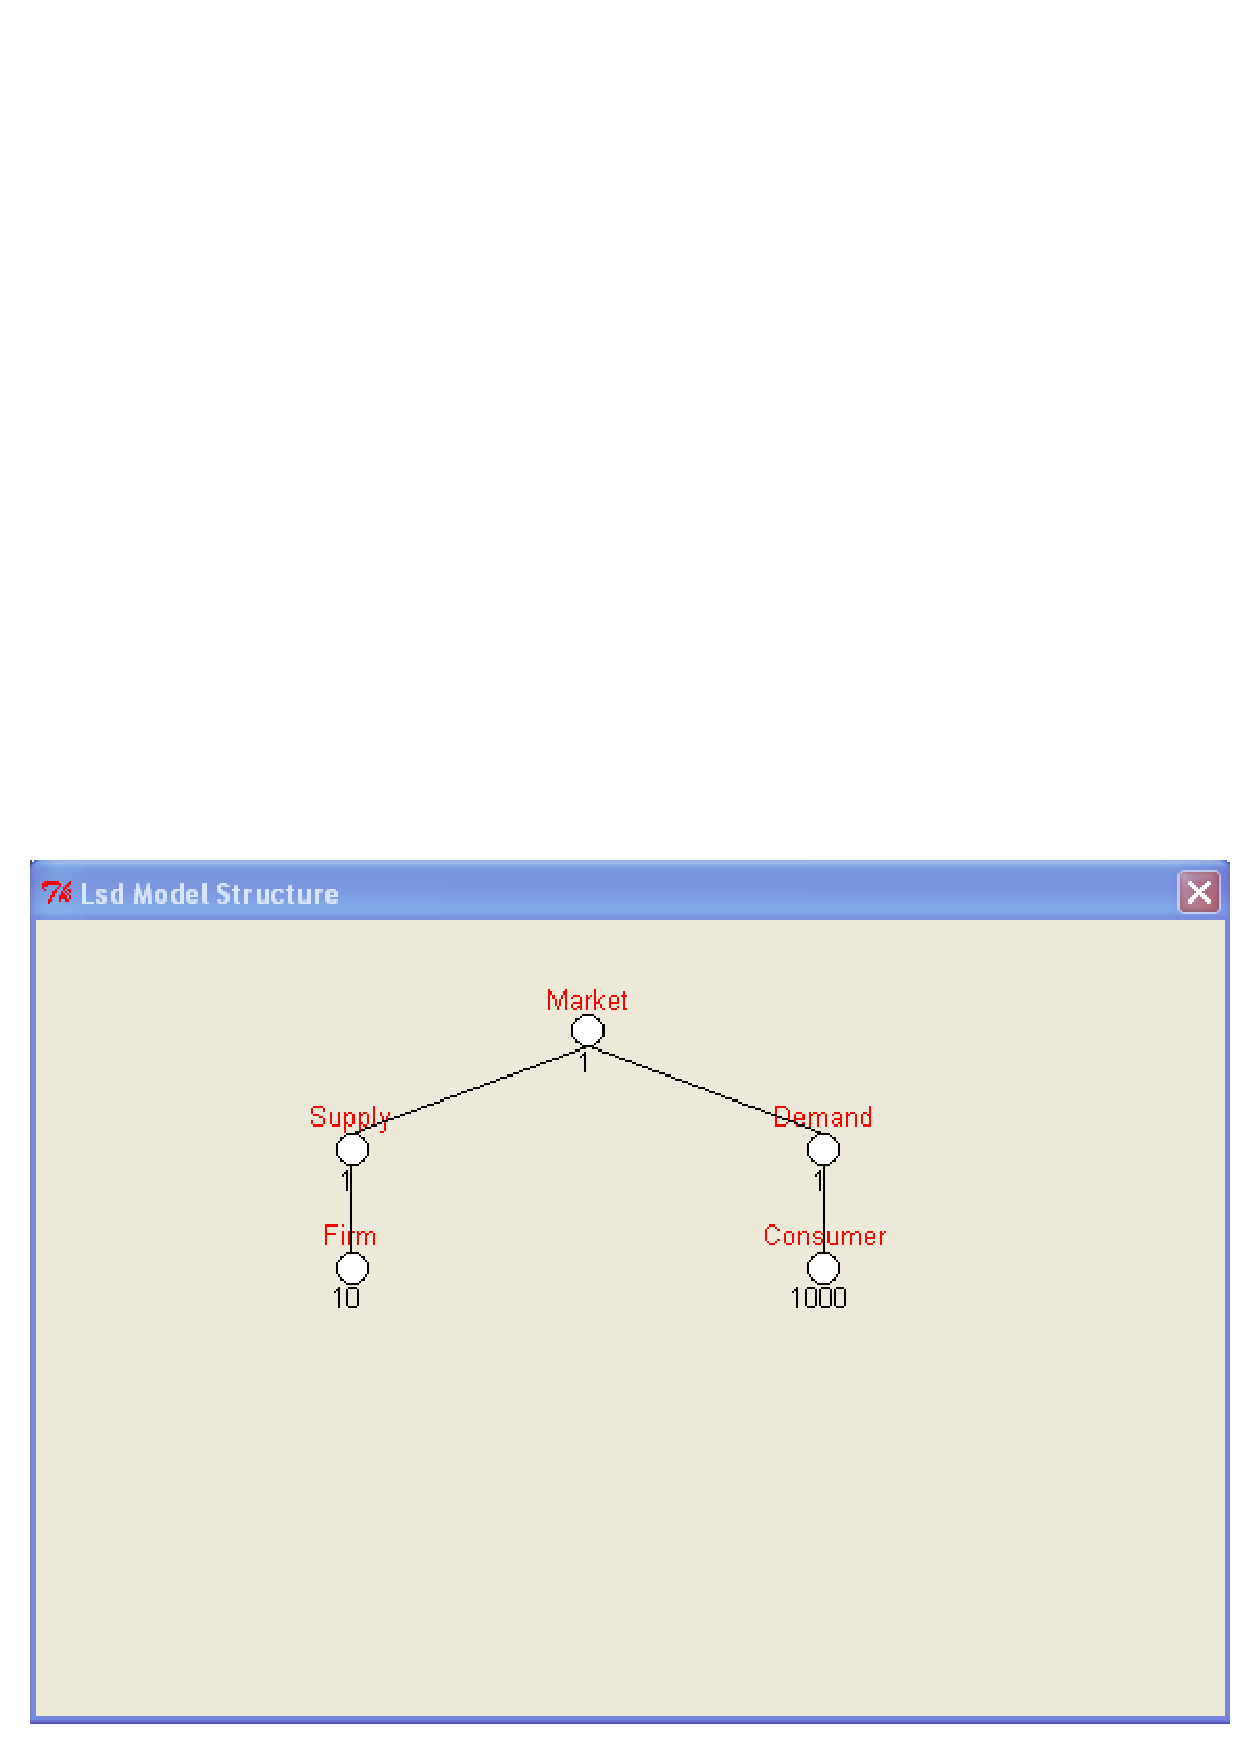
\includegraphics[width=12cm]{abmobj.pdf}}
  \caption{\small Object structure of an model. Object \lsd{Market} contains \lsd{Supply} and \lsd{Demand}, which, respectively, contain \lsd{Firm} and \lsd{Consumer}.}
   \label{fig:abm}
\end{figure}

Let's assume that consumers choose the different products randomly, with the probability of choosing each firm being proportional to a firm's parameter, call it \lsd{Quality}. That is, the probability for choosing the generic firm $i$ should be equal to $p_i=\frac{q_i}{\sum_j q_j}$. The \LsD equation for such code is:

\begin{minipage}[ht]{10cm}
\small
\begin{verbatim}

EQUATION("Choose")
/*
Choose on of the product in the descending Firm's objects
*/
cur=RNDDRAW("Firm","Quality");
v[0]=VS(cur,"IdFirm");
RESULT(v[0] )

\end{verbatim}
\normalsize
\end{minipage}
 
This equation uses the \LsD function \code{RNDDRAW(``ObjLab'', ``Prob'')}, which chooses randomly one of copies of objects called \lsd{ObjLab} with probabilities proportional to the element \lsd{Prob}. This function expects that the variable \lsd{Choose} is contained in an object that contains a set of objects labelled as indicated. It sums up all their values for \lsd{Prob} (which must be non-negative) and assigns to each element the probability of being chosen.

The \LsD function \code{RNDDRAW(``ObjLab'', ``Prob'')} returns a pointer, that is, the copy of the object selected, so that the equation uses \code{cur}, to store it. We have already encountered this element before: it does for objects what the local C++ variables \code{v[i]} do for numerical values. In practice, it stores temporarily a specific object, so that the modeller can then operate on them. In our case, the equation reads from the object a parameter, \lsd{IdFirm}, which supposedly is an identification for firms with different values for each object \lsd{Firm}. This value is returned by the equation.

The code for this equation is a rather simple and straightforward representation for the consumers' behaviour. However, we have a problem. In fact, comparing the code for the equation and the object structure we defined before, it is not obvious where the variable \lsd{Choose} should be located. In fact, it clearly represents the behaviour of consumers, and hence we may consider placing it there. On the other hand, the grammar of the equation requires the variable to be placed on an object containing the firms, which is not the case of the objects \lsd{Consumer}. 

This problem is one of the many cases where the very building of a model forces to think carefully of the reality simulated. The necessity to implement a logically consistent model will clarify how the actual system works, and will also suggest solutions to the problems of modeling it.


We may solve our problem by storing many different sets of copies of the firms descending from each consumer. In this case, we are implicitly representing each consumer as having her own perception of the firms, different from that of all other consumers. This approach may be necessary if we want to develop a model in a specific direction. But this approach implies a lot of duplication, and, at least for now, we need not to differentiate all the consumers. We are rather representing several identical consumers who, in turn, ``go shopping'' and choose one product. This is the key to solve the modelling problem we have.

We can place \lsd{Choose} in the object \lsd{Supply}, and then placing a variable in consumer, say \lsd{ProductChosen} which simply calls \lsd{Choose} and copies its result.


\begin{minipage}[h]{10cm}
\small
\begin{verbatim}
EQUATION("ProductChosen")
/*
Product used by the consumer
*/
v[0]=V("Choose");
RESULT( v[0])

\end{verbatim}
\normalsize
\end{minipage}

In this way we have both requirements satisfied. The consumers' variable \lsd{ProductChosen} will contain the identification of the firm that sold her the product, and \lsd{Choose} can be placed within \lsd{Supply}, being able to ``see'' all the descending firms. This way manages to represents formally in the model the existence of many, independent consumers, each of them exploiting the ``shopping'' method, located where all firms are accessible. But this model still cannot run as intended, if we don't pay attention to a serious potential error. Before discussing this, however, we'd better construct the full model configuration.

Compile this \LsD model program and initialize the configuration with 10 firms and 1,000 consumers. Insert variable \lsd{ProductChosen} in \lsd{Consumers} and parameter \lsd{Quality} in \lsd{Firm}. Initialize parameters \lsd{Quality} with increasing values from 10 to 19. Now we can discuss \lsd{Choose}; we know it should be located in \lsd{Supply}, providing each consumer with a product id, which will be stored in variable \lsd{ProductChosen}. But \lsd{Choose}  cannot be defined as a variable. In fact, variables in a discrete difference equation models are labels associated to a single value within each time step, and we know that the \LsD model manager ensures that the code for the equation of a variable is computed once, and only once, for each $t$. If \lsd{Choose} were defined as a variable, at a time step it would execute its code once, and the resulting value (the id of the chosen firm), would be returned to each consumer. But this is not what we meant: we designed the model to have the code for \lsd{Choose} be re-executed every time a consumer needs to buy a product, many times within the same time step. On the other hand, \lsd{Choose} is not a variable that we may be interested to observe, for example plotting its time series result: its meaning is to serve consumers, not to take independently values.

\LsD allows to define other numerical elements, besides variables and parameters. They are called \textit{functions}: labels associated to a piece of code, much like variables, but that are not constrained to be computed once at every time step. The code for a function is executed only, and every time, the code for an equation in the model requests its value. This is the nature of \lsd{Choose}, which is a sort of ``extension'' of the variables \lsd{ProductChosen}; the latter must be computed only once, but the former needs to re-execute its code every time its value is requested. Note also that \LsD does not compute the code for a function unless it is requested, differently from variables. 

Place in \lsd{Supply} the function \lsd{Choose}, using menu \menu{Model/Add a function}. Now we can run the model. We can expect firms with higher quality selling more than firms with lower quality. But how can express this results?

\section{Analysis of Results: Histograms}

In this paragraph we explore one of the features of the Analysis of Results, motivated by the little information produced by the model so far. Later we will develop the model so to generate more sensible and clearer results, so, uninterested readers, may skip this paragraph.

Our model is pretty basic, containing only one variable and its ``extension'' as a function. This variable being the only result, mark it to be saved, run the simulation and open the Analysis of Result window. We will have the 1,000 series of the \lsd{ProductChosen} variables available, but they are of not much use, since they assume only integer values between 1 and 10. If we tried to plot the time series of one of these variables we will be shown a line jumping at different integers for each time step, indicating the id of the product chosen by that consumer for the time step. What we can do, however, is to count the different values assumed by the variable through time. Select one variable and click on \menu{Histograms}. A new window will ask the number of classes to use; type in 10 (since there are 10 values we are interested into, the id of the existing firms). 

The resulting window as contains as many columns have been requested, 10 in our case. The horizontal axis refers to the variable measured, in our case the integers from 1 to 10. The height of the columns refer to the frequency by which values were registered. We can expect that higher values, referring to the id of higher quality firms, should be more frequent than lower id's. 

The histograms are formed in the following way. The system computes the range of variability of the series considered; in our case it ranges from 1 to 10 (unless one of the extreme is never reached, but this is highly unlikely). This range is then divided in evenly spaced sub-ranges, whose number is decided by the user (we asked for 10). Then, the series is scanned again and system counts how many times the variable values fall into each of the sub-ranges, or classes, defined. Such values are then used for the height of the columns. Note that moving the mouse over one of the classes shows, in the lower left corner of the window, information about the class.




However, we have considered the results of only one consumer, over 100 periods, therefore it is likely to produce high random variability. Try to generate histograms for the same variable using only two classes. Doing this you group together all the results in the first half of the range. Notice that the lowest value of the vertical axis is automatically set on the frequency of least frequent class, so that there will be at least one ``empty'' class. Users can change this option removing the automatic vertical scaling, and using any minimum value.

Time series histograms can be generated for only one variable. A normally more sensible use of histograms is to consider a large set of series and compute the frequency at a given time step, that is, making a cross-section analysis. Remove the series you were using, and select all of them. Use the ``batch selection'' system by clicking with the right button of the mouse on the series to speed-up the process. Change the option on the lower right part of the window from \menu{Time Series} to \lsd{Cross Section}, and press the \menu{Histograms} button.

Now you are requested two types of information. One, as before, concern the number of classes to use; type in 10 in the second entry. The other concern which time step should be considered. By default the system suggests the latest time step available, 100 in our case, and you can leave this value.

The resulting graph will contain the frequencies computed at the indicated time step computed over all the variables considered. The larger sample use is now more likely to produce a representation to the expected results: firms with higher id's (i.e. those with better quality) have higher frequency than those with lower id's.

Though these results confirm the proper functioning of the model, we may want to extend the model to express more clearly this result, besides making it more interesting.

\section{\LsD equations: the calling object \code{c}}
An obvious extension of the model consists in implementing a variable to compute the number of customers for each firm. The most straightforward code for such a variable consists in having firms scanning all the consumers and counting how many of them have the consumers' variable \lsd{ProductChosen} identical to the firm's own \lsd{IdFirm}\footnote{This is obviously highly inefficient, though, given the speed of \LsD simulations, it will not be too onerous, at least for relatively small number of consumers. In any case, we will later discuss how to optimize the model to speed up the execution.}.

We encounter again a familiar problem. On the one hand we need a variable located in the firms, but this variable needs to be able to access all the consumers. We know how to solve this problem: place a variable in \lsd{Firm} and a function in \lsd{Demand}, where the function performs the actual counting and the variable simply store the result. Call \lsd{Num} the variable to be placed in \lsd{Firm}, whose equation can be written as follows.

\begin{minipage}[h]{10cm}
\small
\begin{verbatim}
EQUATION("Num")
/*
Number of customers of the firm
*/

RESULT( V("ComputeSales"))

\end{verbatim}
\normalsize
\end{minipage}


For the function \lsd{ComputeSales} contained in \lsd{Demand} we have, however, an additional problem. The function will be executed on request by every firm, but it needs a piece of information from each of them. The function  \lsd{Choose} we used before did not need to know which consumer had requested its value: the result was identical for each consumer. While for \lsd{ComputeSales} this is not the case: the code needs to provide different results depending on the firm that requested it. How can this be expressed? Let's see the code for the function.

\begin{minipage}[h]{10cm}
\small
\begin{verbatim}
EQUATION("ComputeSales")
/*
Compute the customers for each firms
*/
v[0]=VS(c,"IdFirm");
v[2]=0;
CYCLE(cur, "Consumer")
 {
  v[1]=VS(cur,"ProductChosen");
  if(v[0]==v[1])
   v[2]++;
 }
RESULT(v[2] )

\end{verbatim}
\normalsize
\end{minipage}

The first line of the equation is what allows the function to behave differently for each firm. It uses the usual \code{VS(...)} \LsD function, requesting the value of an element (\lsd{IdFirm}) from a specified object. The particularity is the object specified, \code{c}. This a pointer, that is, a C++ ``variable'' meant to contain objects instead of numerical values, as the \code{cur}. The difference is that \code{c} cannot be set by the modeller, as \code{cur} requires, but is automatically set by the \LsD model manager: it contains the \textit{\underline{c}aller} object, that is, the object containing the variable requesting the value for the code under execution. In this case, we have the variable \lsd{Num} stored in \lsd{Firm}; when one of these variables is executed it calls \lsd{ComputeSales}, and the equation for this function is given the object containing the specific object \lsd{Firm} that have its \lsd{Num} under computation. The modeller can use this object referring to \code{c}. As a result, the equation for \lsd{ComputeSales} is able to access all the content of that specific copy that requested its value.

The computational elaboration of the equation is rather obvious. Firstly, the local variable \code{v[2]} is set to zero. Then all consumers are scanned, using the \code{CYCLE(...)} command. For each consumer we read its value of \lsd{ProductChosen}; if this value is identical to the value of \code{v[0]}, then we increase the counter \code{v[2]}.

To perform these operations we use two C++ expressions. The \code{if(...)} command is a conditional statement: it control whether the condition expressed within parentheses is true or false. If it is true, the following line is executed, otherwise it is skipped. Note that the condition uses the expression \code{==}, which differs from \code{=} in that the latter is the assignment command in C++. Confusing the two generates dangerous errors. In fact, the ``condition'' \code{v[0]=v[1]} is always true, since it means: ``place in \code{v[0]} the value of \code{v[1]}'', which C++ interpret as a true value.

The counter assignment, executed under condition of \code{v[0]} and \code{v[1]} being equal, is expressed using a piece of C++ jargon. The \code{++} placed after a variable is interpreted as \code{v[0]=v[0]+1}. It is merely a formatting rule, allowing to simplify the writing (and reading) of the code. 

We can now run the model. Save the configuration, containing the new variable and function, and close the \LsD model program. Place the code for the new elements in the equation file and compile the new \LsD model program using \menu{Model/Run}. Once this appears, load the configuration, ensuring that variables \lsd{Num} are marked to be saved, and run the simulation. You should now to be able to see the series for \lsd{Num} representing the number of consumer for each firm,


\section{More on the \LsD Debugger}
Our model is getting more elaborated. Let's imagine that something is going wrong or, in any event, that we want just to control that simulation runs as it is expected to. Before running a simulation open the simulation setting (\menu{Run/Sim. Setting}). Place 50 in the entry corresponding to \menu{Insert Debugger at}. Then, mark the function \lsd{ComputeSales} as being debugged. Now run the simulation and it will show the \LsD debugger immediately after the marked function just completed its code at time step 50.

The window will show the content of the object containing the element that interrupted the simulation, \lsd{Demand} in our case. We know that this is a function, which can be executed only if a variable \lsd{Num} requested its value. To confirm this, press the button \menu{Print stack}, in the first row of buttons. The \menu{Log} window will show the state of the stack at the moment the simulation was interrupted, showing the following message.

\begin{minipage}[h]{10cm}
\small
\begin{verbatim}

List of Variables currently under computation.
(the first-level Variable is computed by the simulation manager, 
while possible other Variables are triggered by the lower level ones 
because necessary for completing their computation)

Level	Variable Label
2	ComputeSales
1	Num
0	\LsD Simulation Manager

\end{verbatim}
\normalsize
\end{minipage}

It means that \lsd{ComputeSales} have been executed as ``stack level'' 2, as a consequence of being requested by a variable \lsd{Num}. 

The debugger allows to observe the values of all the temporary C++ variables \code{v[i]} with their value at the end of the just completed equation. Press the button \menu{v[...]} in the debugger window, the second from the left in the first series of buttons, and a new window as in figure \ref{fig:v} will appear.


\begin{figure}[ht]
  \centering
 \fbox{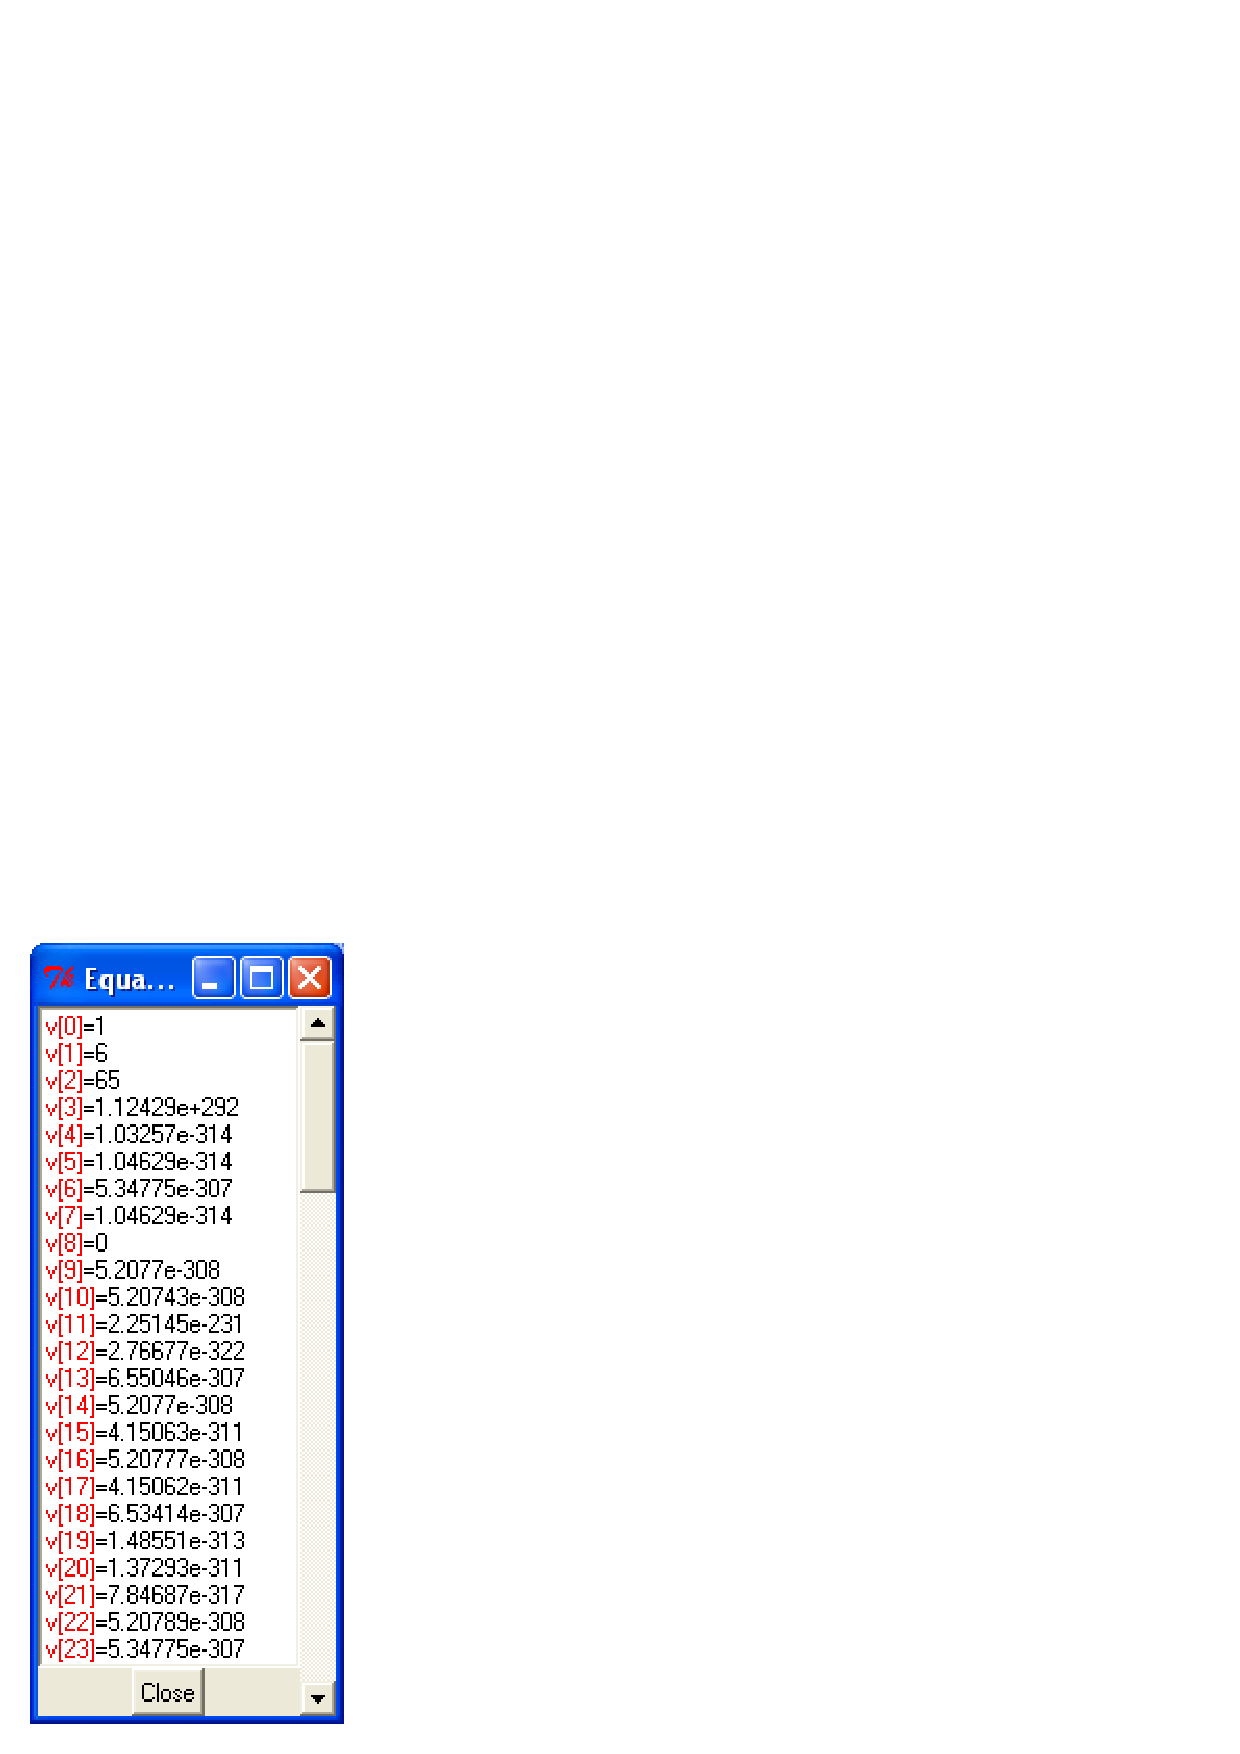
\includegraphics[width=3cm]{v.pdf}}
  \caption{\small Series of the \code{v[i]} provided by the debugger.}
   \label{fig:v}
\end{figure}

Of the values shown, only the first three, \code{v[0]}, \code{v[1]} and \code{v[2]} are used in the simulation:\footnote{The other ones express a value reflecting the state of the memory allocated, so that they are, to all effect, random values over the entire set of real numbers. This also shows why we need to set to zero the counter \code{v[2]}, since the content of these variable is impredictable.} \code{v[2]} is the counter, so that it has the same value of the \lsd{ComputeSales} value; \code{v[1]} is the product used by the last consumer; and \code{v[0]} is the id of the firm requesting the computation of \lsd{ComputeSales}.

We can use the debugger to control whether these values are indeed correct. Press the button \code{Caller}, second from right in the second row of buttons. The debugger will be moved to show the \textit{caller} object, that is, the one containing the variable that triggered the debugged element. In our case, it is the very first copy of the \lsd{Firm}, with \lsd{IdFirm} equal to 1. Notice that variable \lsd{Num} will be not udpated at the $50^{th}$ time step, because the simulation stopped just after \lsd{ComputeSales} completed its equation, and therefore it has not provided the result to \lsd{Num}, which appears still as not computed.

Use then the arrows to go up the firms (\lsd{Supply}), right (\lsd{Demand}) and down (the first \lsd{Consumer}). Press now the button \lsd{Last}; the debugger will then move to the last object of the set of \lsd{Consumer}. The variable \lsd{ProductChosen} for this consumer will be the same as that indicated by \code{v[1]}, since this C++ local variable was loaded with this value in the last round of the cycle for \lsd{ComputeSales}.

Clicking on the button \menu{Step} will cause the model to continue the simulation until the next equation for an element to be debugged is encountered. In our case, we have only the function \lsd{ComputeSales} set to interrupt a simulation run for debugging, and thus we will see again the debugger showing the \lsd{Demand} object, at, again, the same $50^{th}$ time step. This would be impossible if \lsd{ComputeSales} where defined as a variable, since variables would be computed once, and only once, at every time step. But this being a function, its code is re-executed when another equation requires its values. Press \code{Caller}, and you will see the object for the second \lsd{Firm} shown by the debugger, since it is its own copy of \lsd{Num} which caused \lsd{ComputeSales} to be (re-)computed.

Press \code{Run} to continue the simulation until its natural completion.

\section{Extending the model}

We have now a model producing the sales of each firm as a function of a (rather basic) consumers' behaviour. To analyse in detail the results we need to generate some statistics on the model results. Though statistical packages may be used for the purpose, feeding them with the raw model results (\lsd{Num} in our case), it is generally simpler to write the statistics as \LsD variables directly in the model. In fact, C++ is faster than any statistical package, and moreover we can observe directly the statistics at run time, speeding up the process of analysing the results. Moreover, writing the code for the most of statistical indicators is rather trivial, and we may use this as a further exercise.

Let's implement the code computing an indicator of concentration for the market shares. Consider the Herfindahl index, expressed as:

\[
H=\displaystyle \sum_{i=1}^N ms_i^2
\]

where $ms_i$ are the market shares of firm $i$. Actually, a better indicator is the inverse of the Herfindahl index, $InvH=1/H$, which becomes an index of dispersion. This indicator (which is always larger than 1), reports the equivalent number of firms with identical shares of the market that would generate the same concentration measured in the actual market.

To write this equation in \LsD we need also to write the equations for the market shares and total sales.


\begin{minipage}[h]{10cm}
\small
\begin{verbatim}

EQUATION("ms")
/*
market shares
*/

v[0]=V("Num");
v[1]=V("TotalNum");
RESULT(v[0]/v[1] )

\end{verbatim}
\normalsize
\end{minipage}

The equation for market shares pose no problem, being a ratio between \lsd{Num}, which the model already computes, and \lsd{TotalNum}, that we still need to implement. Its equation is:

\begin{minipage}[h]{10cm}
\small
\begin{verbatim}

EQUATION(''TotalNum'')
/*
Sum of all the sales
*/

RESULT(SUM(''Num'') )

\end{verbatim}
\normalsize
\end{minipage}

The code for \lsd{TotalNum} uses one of the \LsD functions, \code{SUM(''Lab'')}. This function returns the sum of all the elements \lsd{Lab} contained in the group of objects descending from the object containing the variable. Therefore, in our case, we need to place \lsd{TotalNum} in the object \lsd{Supply}\footnote{We may even place this variable in \lsd{Market}, since it is an object superior to the ones containing \lsd{Num}.}.


As for the inverse Herfindal we use the usual system to cycle throughout the firms.


\begin{minipage}[h]{10cm}
\small
\begin{verbatim}

EQUATION("InvHerf")
/*
Inverse Herfindal index
*/
v[0]=0;
CYCLE(cur, "Firm")
 {
  v[1]=VS(cur,"ms");
  v[0]+=v[1]*v[1];
 }
v[2]=1/v[0];
RESULT(v[2] )

\end{verbatim}
\normalsize
\end{minipage}

Notice the C++ expression \code{v[0]+=v[1]*v[1]}, which is a short version equivalent to \code{v[0]=v[0]+v[1]*v[1]}. As we have seen before, this equation simply cumulates in \code{v[0]} some values for each firm (in our case, the square of market shares). The result is simply the inverse of the cumulated values.


We can now compile and run the \LsD model program, if there are no compilation errors. If you typed the three equations, than the probability of typos, or forgetting elements, will be rather high. Consider that error messages can be spurious. If, for example, the code lacks a closing parenthesis, the compiler is likely to generate many errors for the legal code following the missing character. Therefore, if the compiler signal many errors, try always to fix only the very first error indicated in the list (which is the earliest in the file of the equations), and ignore the others. Re-compile and, it is likely that at least some of previously signalled errors have now disappeared from the list.


Once the \LsD model program embedding the equations is running, load the existing configuration and add the variables \lsd{TotalNum} and \lsd{InvHerf} in \lsd{Supply}, and \lsd{ms} in \lsd{Firm}. Mark all of them to be saved and \lsd{ms} to be also plotted at run time.

When you will launch the simulation a new window will appear, called \menu{0 Run Time Plot}. This window generates the time series graph for the variables marked to be plotted at run time. The vertical scale is automatically adjusted, and therefore users should not set the run time options variables with very different ranges of values (say, putting \lsd{Num} and \lsd{ms}), since the vertical scale (topping the thousands) will make all market shares to be squeezed in a unreadable line close to the bottom of the graph.

In any case, the run time windows are useful to provide a quick understanding of the overall results of a simulation run without stopping it and using the analysis of result module.

The results produced in the model reflect the randomness governing the behaviour of consumers, producing fluctuating market shares. However, higher quality firms have consistently higher shares, on average, than lower quality ones, as we may have expected. We can now move to consider how the concentration of the market can be controlled.

\section{Multiple parallel simulations}

An obvious way to extend or restrict the dispersion of the market consists in changing the distribution of qualities across firms. At the moment we initialized the model to have firms with quality ranging from 10 to 19. If we modified this distribution ranging, say, from 10 to 30 or more we would clearly generate higher concentration, since the quality differences will increase the probability of consumers choosing high quality firms.

A less obvious, but, in some cases, more efficient way to model the concentration of shares consists in modifying the transformation of qualities in probabilities. We implemented the model representing the probability of each consumer to choose product $i$ as $p_i=\frac{q_i}{\sum_j q_j}$, where $q_i$ is the quality of the product. Consider the slightly different generation of probabilities as follows: $p_i=\frac{q^\alpha_i}{\sum_j q^\alpha_j}$, where $\alpha$ is a non-negative parameter. Maintaining constant the qualities $q_i$ the lower $\alpha$ the more similar will be the probabilities, while the higher $\alpha$ the steeper will be the probabilities differences. Figure \ref{fig:prob} shows how $\alpha$ affects the probabilities. 

\begin{figure}[ht]
  \centering
 \fbox{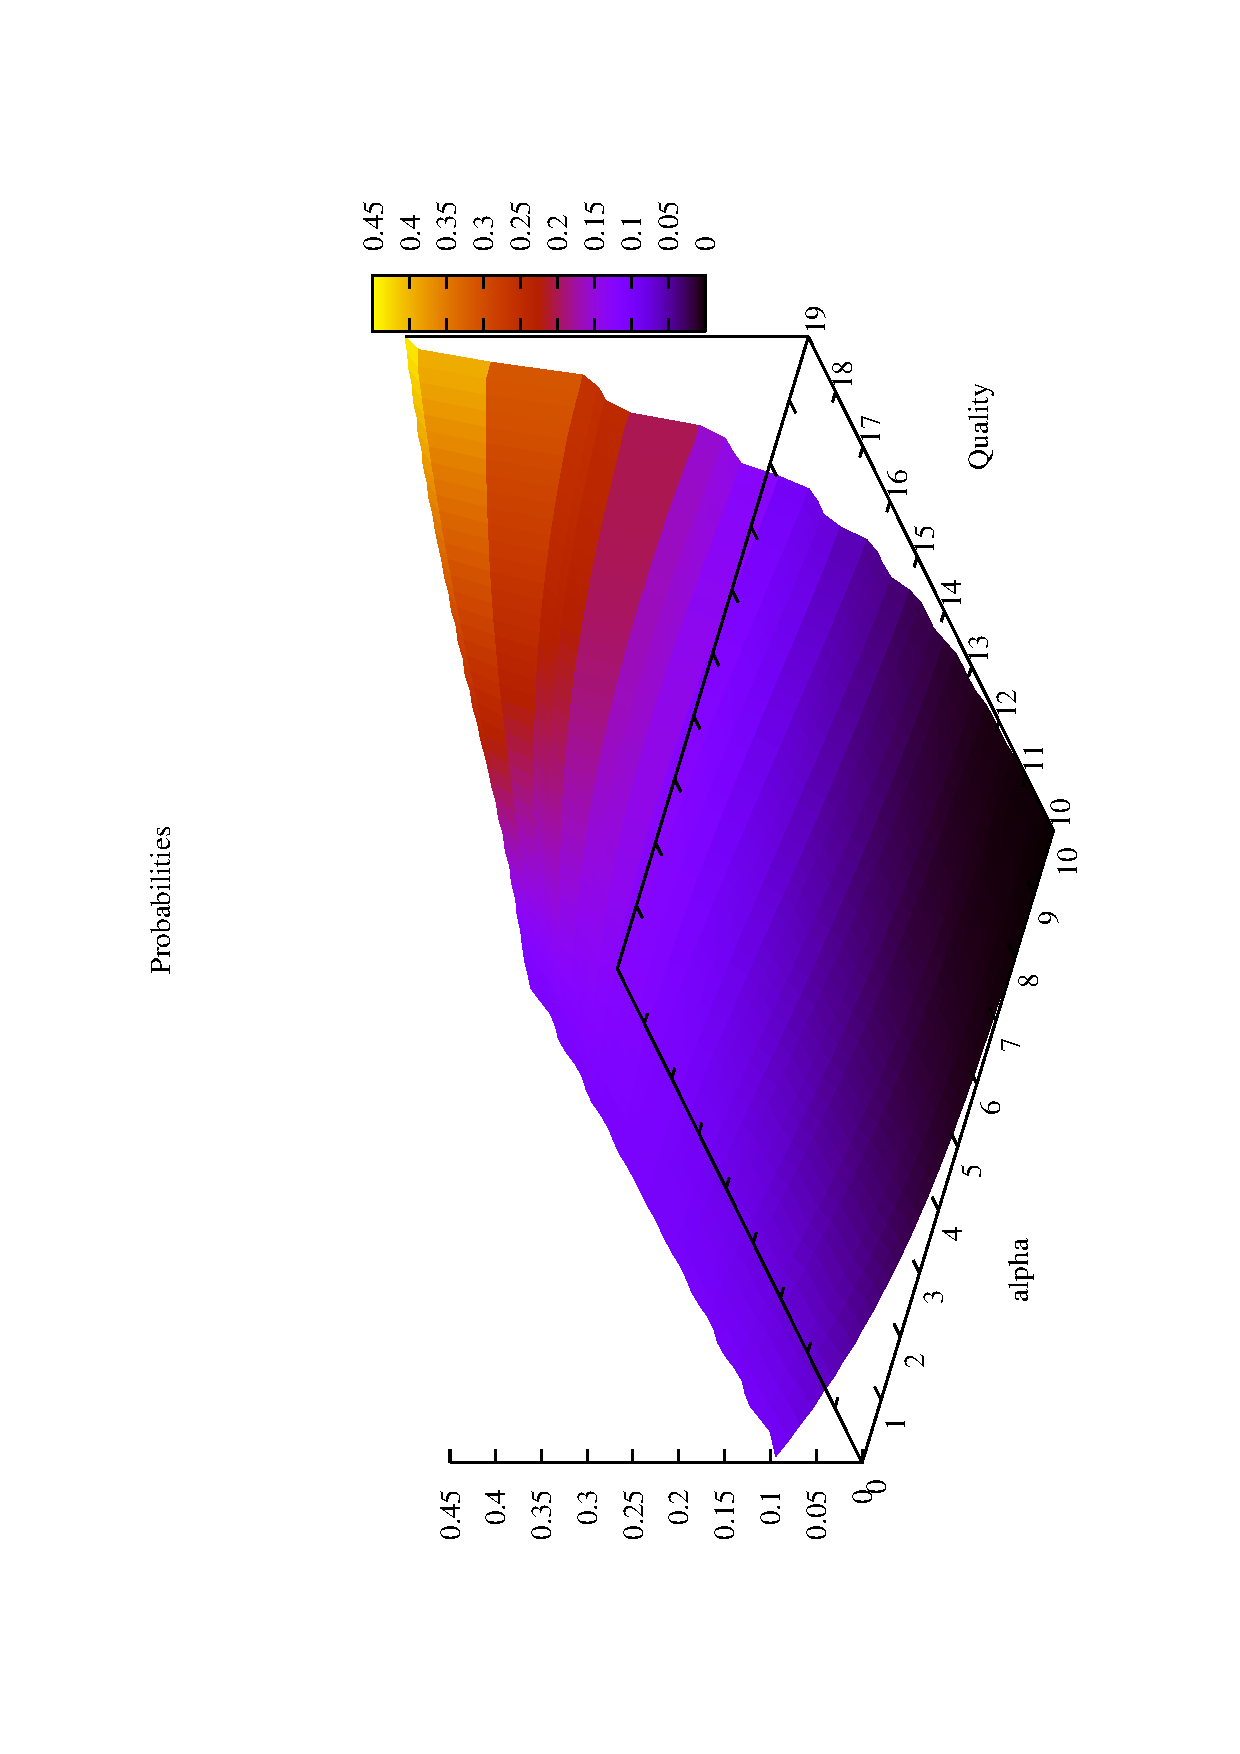
\includegraphics[angle=0,width=12cm]{prob.pdf}}
  \caption{\small Distribution of probabilities for the same distribution of qualities corresponding to different $\alpha$'s. Higher values generate stronger differences of probabilities, while values closer to 0 generate almost identical probabilities.}
   \label{fig:prob}
\end{figure}

The graph\footnote{The figure has been generated with \LsD, after having suitably implemented the equations for the probabilities, and using the 3D features for scatter-plot. Below we will provide details on how to generate these types of graphs.} shows an identical distribution of qualities and different values of $\alpha$, so that summing up across the axis for qualities we always obtain 1. However, lower values of $\alpha$ generate almost identical probabilities (close to 0.1, given that there are 10 firms). Instead, high values of $\alpha$ concentrate the whole probabilities only on the high quality products.



Let's modify the model so that the consumers' choose proportionally to the power \lsd{Quality}$^\alpha$, instead of \lsd{Quality}. Close the \LsD model program and introduce the equation for a new variable, call it \lsd{Visibility}:

\begin{minipage}[h]{10cm}
\small
\begin{verbatim}

EQUATION("Visibility")
/*
Evaluate the visibility of the product for the consumer
*/

v[0]=V("alpha");
v[1]=V("Quality");
v[2]=pow(v[1],v[0]);
RESULT(v[2] )

\end{verbatim}
\normalsize
\end{minipage}

Note the \code{pow(base, exp)}. This function one of the mathematical functions available in \LsD, providing $base^{exp}$, where \code{base} and \code{exp} are two positive real numbers or variables. We also need to change the equation for \lsd{Choose}, replacing the line 

\code{cur=RNDDRAW("Firm","Quality");} 

with 

\code{cur=RNDDRAW("Firm","Visibility");}


Compile the \LsD model program and load the configuration. Since \lsd{alpha} must be identical for all the firms, we can place it in object \lsd{Supply}. Finally, introduce the new variable \lsd{Visibility} in objects \lsd{Firm}. Initialize \lsd{alpha} to 1 and run the simulation. Observe the results, then re-load the simulation and test two runs with \lsd{alpha} equal to 0.1 and equal to 10. As expected, the sales (or market shares) are more concentrated with lower \lsd{alpha}, producing higher dispersions measured by \lsd{InvHerf}, while the opposite happens for high values of \lsd{alpha}. The next step would be to compare the results for a full range of \lsd{alpha}, for example producing a graph reporting the values of \lsd{InvHerf} as a function of \lsd{alpha}.

In order to comparing the results from different simulations, identical in all conditions but for one parameter, there are two possible alternatives. We may generate a simulation, save the results on a file, then change the parameter, re-run the simulation, save the results, and so on. Finally, we may merge all the results and making our comparison. 

This strategy, though technically viable\footnote{\LsD allows to save the results in such a format to be later loaded in the Analysis of Results module, as if they were just produced by a simulation. The operation can be also performed for many different result files, whose content will be then merged in a single result dataset.} is not very efficient. It would require to launch tens of simulations manually and, for each of them, executing the following step: save the results; reload the configuration; change the parameter's value; re-lunch the new simulation run. Though each step takes a few seconds, repeating them, say, 100 times would occupy the modeller for the good part of an hour, in a quite boring activity.

The object structure of \LsD model allows a much simpler and faster strategy: multiply the object \lsd{Market} and assign to each of them a different \lsd{alpha}. A single simulation run will then produce all the data we need to perform the comparison. Each object \lsd{Market} will be independent from the others, in effect representing a separate simulation run. The great advantage of using object, instead of vectors, is that having many \lsd{Market}'s instead of one makes no difference to the equations of the model. The only potential problem we may encounter is that we will have a large number of variables, potentially slowing down the simulation to unacceptable levels, and generating problems to identify variables from different firms and markets. However, the underlining C++ layer of \LsD is able to exploit at best the computational power of the available harwdare, as well as the memory, so that there are rather loose constraints in this respect.

The second potential problem is that we may get confused in dealing with the huge number of variables, not being able to identify related series, as, for example, those generated by the firms in the same market. \LsD avoids such problems by automatically attaching each series with a \textit{tag} identifying uniquely the object to which the series refers to. Moreover, \LsD offers an efficient tool to search and select series on the base of the tags, so to avoid being forced to scan manually thousands of series.

Re-load your configuration and move the browser to show object \lsd{Market}. Opening menu \menu{Data/Set number of obj.} you will be given two options. The first, \menu{All types ...}, allows to show the whole tree of objects of the model. The second, \menu{Only current ...} allows instead to set only the number of objects in the browser, in our case \lsd{Market}. This second option is faster to use when you need to change only one type of objects, so choose this and type in 100. Pressing \menu{Ok} you have generated 100 copies of \lsd{Market}, as shown by the \menu{\LsD Model Structure} graphical representation of the model.

All copies of the newly created objects are identical, but we want to assign different values for \lsd{alpha}. Therefore, move the browser to \lsd{Supply} and select menu \menu{Data/Init. values}. In the resulting window click on the \menu{Set all} button corresponding to the parameter \lsd{alpha}. We can now assign to each copy of this parameter in the different \lsd{Market}'s a different value. Choose the initializing function \menu{Range} and set the values 0.1 and 10 for the extremes. This function computes how many copies of the element to initialize are present in the model, and divides the requested range in evenly-spaced subranges, assigning to each of the elements the extreme for the subranges. See the \menu{Help} button on this window for further details on this and the other initializing functions.

In order to control that the initialization worked as expected you can control on the initial values' window. However, this window is limited to contain a maximum of 100 cells for each element\footnote{The reason is that such a window will become exceedingly ``heavy'', given the large number of elements and their links to the actual C++ representation of the model. Moreover, it can hardly be imagined a user willing to type more than 100 initial values manually. Obviously, the initialization functions apply to every object in the model.}, and therefore, in general, it is not sufficient to control all initial values, when these exceeds this number.

Another interface to control the values contained in the model is the same used for the debugger, which can be also activated to observe the model content before or after a simulation run. Open menu \menu{Data Browse} and you will see the \menu{Debugger} window, but for the button controlling the simulation flow (e.g. \menu{Run}, \menu{Step}, etc.), which are meaningless in this context. Use the arrows to move around the model, controlling that there are actually 100 markets, and each of their supplies has the prescribed values for \lsd{alpha}. Notice that you can move only following the links of the objects; for example, you cannot move from one object \lsd{Supply} to the next object of the same type using the right arrow only. In fact, you will find firstly the \lsd{Demand} contained in the same \lsd{Market} and then the right arrow will not be able to move beyond that. To reach the next object \lsd{Supply} you need to move up to go to the \lsd{Market}, then right to reach the next one, and down to show its own copy of \lsd{Supply}.

\begin{figure}[ht]
  \centering
 \fbox{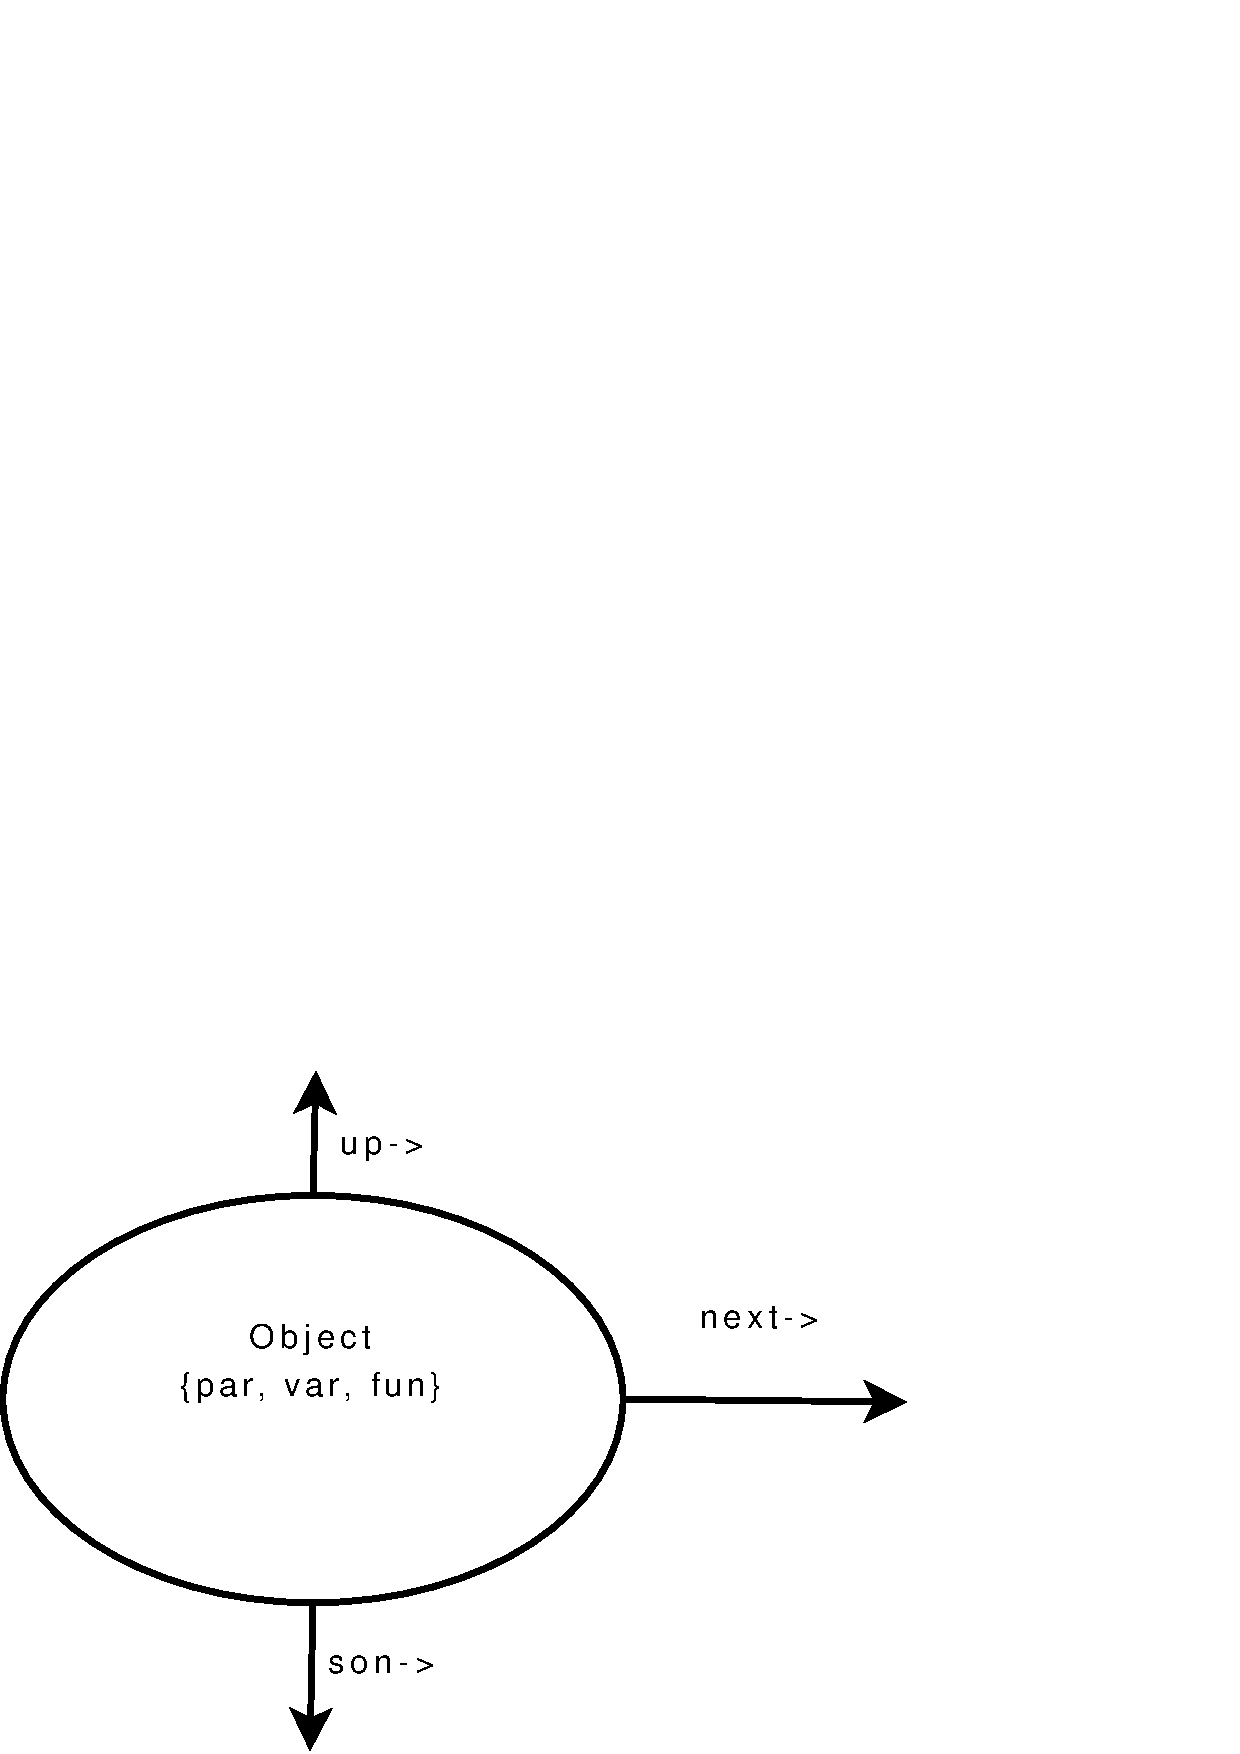
\includegraphics[width=8cm]{object.pdf}}
  \caption{\small Object structure representation in \LsD. An object contains the minimum information possible, besides its content of variables, parameters and functions. In particular, the structural content of the objects, allowing to place the object within the model structure, are only three: \code{son->} indicates the very first copy of the objects descending from it; \code{next->} indicates the subsequent object in the list of the parent object; \code{up->} indicate the ``parent'' object, containing it. The internal \LsD functions exploit these three fields of any object to perform any activity, like searching for variables, showing the objects' content, etc.}
   \label{fig:object}
\end{figure}

The pattern among objects is determined a very limited number of links, which the \LsD functions exploit to travel the model when needing to perform some activities. Figure \ref{fig:object} represents the three only objects that can be access from any given starting object: the one ``up'', containing it; the one ``down'', the first of the descending objects; and the one ``right'', the next in the list of the objects contained in the parent (``up'') object. 


Ensure that \lsd{InvHerf} and \lsd{alpha} are both set to be saved. Also, it is better to remove the options to generate the Run Time Plot. In fact, this option set for the market shares (\lsd{ms} in object \lsd{firm}) would produce a graph comprising 10 x 100=1,000 series. Besides being rather useless, generating such a heavy graph would slow down the simulation. You can use the menu \menu{Run/Remove Plot Flags} to remove any option (``flag'') to plot an element of the model in the Run Time Plot.

The simulation will be quite slow, anyway. Partly this is due to the sheer amount of computation requested: 1,000 consumers per market, each scanned by each of the 10 firms. However, the model we built so far is particularly inefficient, requiring each firm to repeat the cycle through all consumers. This strategy can obviously be improved, as we will see below. Anyway, for the time being we can keep the model as it is and analysing the results produced.

\section{Series tags and advanced selection}

\LsD models allow the generation and saving of so many series that simply identifying the ones to be selected (for example, for plotting) can be all but impossible using only the normal scrolling and clicking\footnote{Relatively complex models may require to analyse several thousands of series.}. In this paragraph we describe the use of the advanced selection system for series in the Analysis of Result module, to be used when the number of series available is too large to use the manual selection.

At the end of the simulation open the analysis of results. We have generated 100 groups of series, one for each \lsd{Market}. Each group contains one series for \lsd{alpha} and \lsd{InvHerf}, plus 10 series for market shares \lsd{ms} and sales \lsd{Num}. Notice the tags generated along the elements' names in the \menu{Series Available} list, a sample of which is shown in figure \ref{fig:tags}.

\begin{figure}[ht]
  \centering
 \fbox{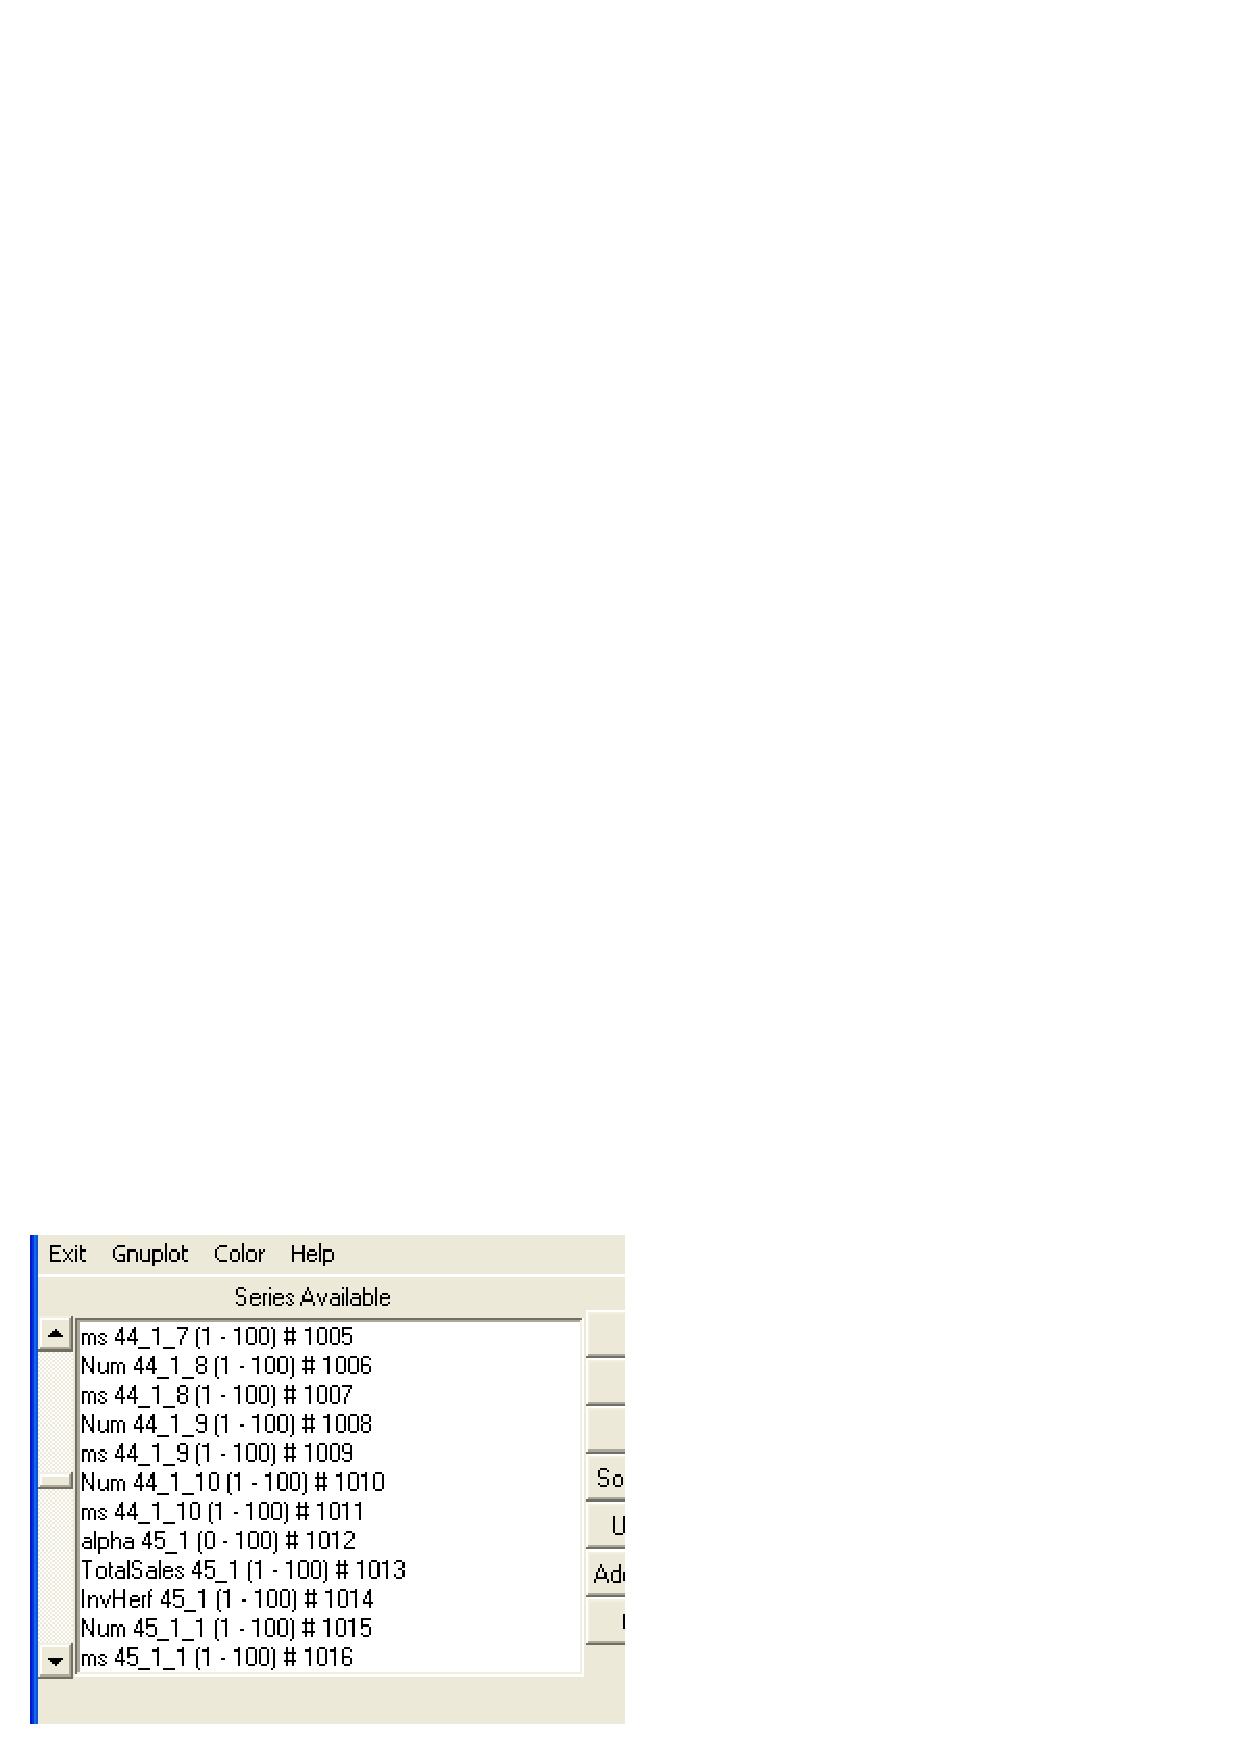
\includegraphics[width=6cm]{tags.pdf}}
  \caption{\small Sample of a numerous set of series available for analysis of results. Each series is indicated with the label of the element it refers to; a tag identifying the copy of its object (see the text); the simulation time span it existed; and a unique identification number.}.
   \label{fig:tags}
\end{figure}

\LsD automatically generates a tagging system in order to identify series from different objects. Each tag includes a number of digits equal to the ``layer'' referring to the object containing the element. The first layer is composed by the objects contained in \lsd{Root}; second layer is composed by the objects contained in first-layer objects, etc. For example, \code{alpha 45\_1} is the series for \lsd{alpha} contained in the $1^{st}$ object (\lsd{Supply}, in a second layer) which in turn is contained in the $45^{th}$ object (\lsd{Market}, first layer). Series from firms (third layer, contained in \lsd{Supply} and \lsd{Market}) use three digit tags for the \lsd{Market}, \lsd{Supply} (always 1, since the model contains only one copy per market) and \lsd{Firm}.

As we have already seen, clicking with the right button of the mouse on a series creates a new window allowing the use of selection criteria concerning all the series sharing the label of the series considered. For example, right-clicking on a series for \lsd{ms} in our model generates the window shown in figure \ref{fig:selectionb}.


\begin{figure}[ht]
  \centering
 \fbox{\includegraphics[width=8cm]{selectionb.pdf}}
  \caption{\small Selection criteria for the series \lsd{ms}. Since market shares are contained in objects located in the third layer, the selection via tags permits to use three digits for, respectively, the (\lsd{Market}, \lsd{Supply} and \lsd{Firm}. }.
   \label{fig:selectionb}
\end{figure}

The first option (set by default) allows to select all the series with the label specified. The second option makes use of the tagging system. The user can specify in the cells located in the box for the option \menu{Select for series' tags} any desired value. The system will compare the values in each cell with those of the series, applying the condition specified in the lowest part of the window, \menu{Set condition to meet}. For example, the criterion used in the figure requires to select all the series with label \lsd{ms} having the value of 23 in the first part of the tag. Since this part identifies the markets, the result will be to select all \lsd{ms} contained in the objects \lsd{Firm} in the $23^{rd}$ market. Notice one may change the condition to meet; instead of equality one may for example select \menu{Larger >}, so that the selection will include all the \lsd{ms} from the market 24 included until the last market, 100. It is also possible to fill more than one cell: the selection will include the series satisfying all the conditions for each filled cell. Empty cells are supposed to be always satisfied.

Besides using the tag system, it is possible to use a further selection system, based on the values of another series in the same or related object. For example, this third option allows to select all \lsd{ms} located in objects containing specific values for \lsd{Num} at a given time step. Also, it is possible to select the market shares contained in firms part of a market with specific values for \lsd{alpha}.

Selecting the third option \menu{Select for values in another series} it is necessary to indicate the label of one of the existing series, a time step and a comparison value. The system will then associate the series under selection (in our example, \lsd{ms}) with the series indicated. The association is based on the tags, that is, each copy of the series under selection will be associated to a copy of the indicated series sharing the same tag. Then, the system controls if the indicated series (at the time step specified) has a value meeting the condition with the comparison value: if the condition is met, the series is selected. Try, for example, to select all \lsd{ms} such that the values of \lsd{alpha} at time step 100 is larger than 5. The \menu{Series Selected} will then contain all market shares from the $51^{st}$ market and following, since these are the markets containing \lsd{alpha} satisfying the indicated condition.

A similar system can be used clicking with the right button of the mouse on the \menu{Series Selected} list box. In this case, the system add to the selection a group of series, for possible removal.

\section{Cross-section scatter plots}

In this paragraph we present the use of the Analysis of Results module to generate scatter plots, that is, graphs having two variables on the two axes and reporting a point at the coordinates indicated by two the elements of two. Such graphs can be generated using either a time series perspective or a cross-section one. In the time-series case you define a series whose values will appear on the horizontal axis and one series that, for the same time step, generates the vertical coordinate. In the cross-section case you need to select two blocks of series that, at a given time step, will produce the horizontal coordinates (the first block) and the vertical one (the second block). Obviously, the two blocks must have the same number of series.

We have generated now a series for \lsd{alpha} and \lsd{InvHerf} from each market. Select firstly all the series for \lsd{alpha} and then all the series for \lsd{InvHerf}. In the \menu{Series Selected} you will find therefore 200 series in total. Select the plotting options (lower right panel of the Analysis of Results window) for \lsd{Points},  \menu{Cross-section} and \menu{XY plot}. Click then on the button \menu{Plot}.

\begin{figure}[ht]
  \centering
 \fbox{\includegraphics[width=4cm]{xycs.pdf}}
  \caption{\small Options to generate a cross-section (i.e. same-time) scatter plot.}.
   \label{fig:xycs}
\end{figure}

The first entry defines the time step to consider, by default the latest available. Each series will provide its value referring at the time step indicated here. The last entry requests the number of ``dependent'' variables, those to be reported on the vertical axis. The system will read the series in ``blocks'', defined on the basis of their positions in the \menu{Series Selected} list box (and independently from their label). If there is only one dependent variable the system infers that there are two blocks: the first half of the series is to provide the values to be measured on the horizontal axis, and the the second half those for the vertical axis. Inserting 2 dependent variables the system divides the series selected in three blocks, the first for the horizontal axis and the others for two (reciprocally independent) variables to be plot on the vertical axis.

In general, assume that there is 1 dependent variable, that there are $N$ series in the \menu{Series Selected}, and that $v_{t}^i$ indicates the value at time $t$ of the series in $i^{th}$ position in the series selected. In this case, there will be $\frac{N}{2}$ points plotted in the graph with coordinates:

 $(v_t^1, v_t^{\frac{N}{2}+1}); (v_t^2, v_t^{\frac{N}{2}+2}); ...; (v_t^i, v_t^{\frac{N}{2}+i}); ...; (v_t^{\frac{N}{2}}, v_t^{N}) $
 
 If there one indicates 2 dependent variables there will be two ``variables'' plotted in the graph, each comprising $\frac{N}{3}$ points. The first will have coordinates:
 
 $(v_t^1, v_t^{N\frac{1}{3}+1}); (v_t^2, v_t^{N\frac{1}{3}+2}); ...; (v_t^i, v_t^{N\frac{1}{3}+i}); ...;
 (v_t^{N\frac{1}{3}}, v_t^{N\frac{2}{3}}) $
 
 The second will have the same horizontal values, and the last block as vertical ones:
 
 $(v_t^1, v_t^{N\frac{2}{3}+1}); (v_t^2, v_t^{N\frac{2}{3}+2}); ...; (v_t^i, v_t^{N\frac{2}{3}+i}); ...; (v_t^{N\frac{1}{3}}, v_t^{N}) $
 

Obviously, the user can place as many dependent values as necessary. The system will control that the number of series selected is a multiple of this number plus 1. Moreover, the option window above will show the number of points resulting from the indicated number of dependent variables.

Accepting the default options we will create a scatter plot graph having the values of \lsd{alpha} on the horizontal line and the values of \lsd{InvHerf} measured on the vertical axis. Clicking on button \menu{Ok}, the system will generate the data necessary for \textit{gnuplot} to generate the graph\footnote{Gnuplot is a graphical package available for free (see its distributional license) for Linux and Windows platforms. The distribution of \LsD for Windows includes a copy of this package. \LsD uses Gnuplot to generate all scatter plots.}. However, before actually seeing the graph, a new window offers another option. The graphs generated by gnuplot can be embedded in standard \LsD graph windows, exploiting their facilities as, for example, exporting the graphs in postscript files. However, the translation produces a lower quality graph. Alternatively, it is possible to generate the graph in directly as a gnuplot result, external to \LsD, obtaining a higher quality. In this latter case, the graph window will not be under control of \LsD (e.g. closing \LsD the window will remain open), and there will be a button-only window closing the gnuplot graph\footnote{Users may access gnuplot directly by opening its shell from menu \menu{Gnuplot/gnuplot}. Any scatter plot graph generates also the script necessary to create the graphs in gnuplot (extensions \textit{.gp}), that users can customize to change titles, variable names, etc.}.


Pressing \menu{Yes} (i.e. generating a low quality graph embedded in \LsD window) will generate the graph reported in figure \ref{fig:alpha}.

\begin{figure}[ht]
  \centering
 \fbox{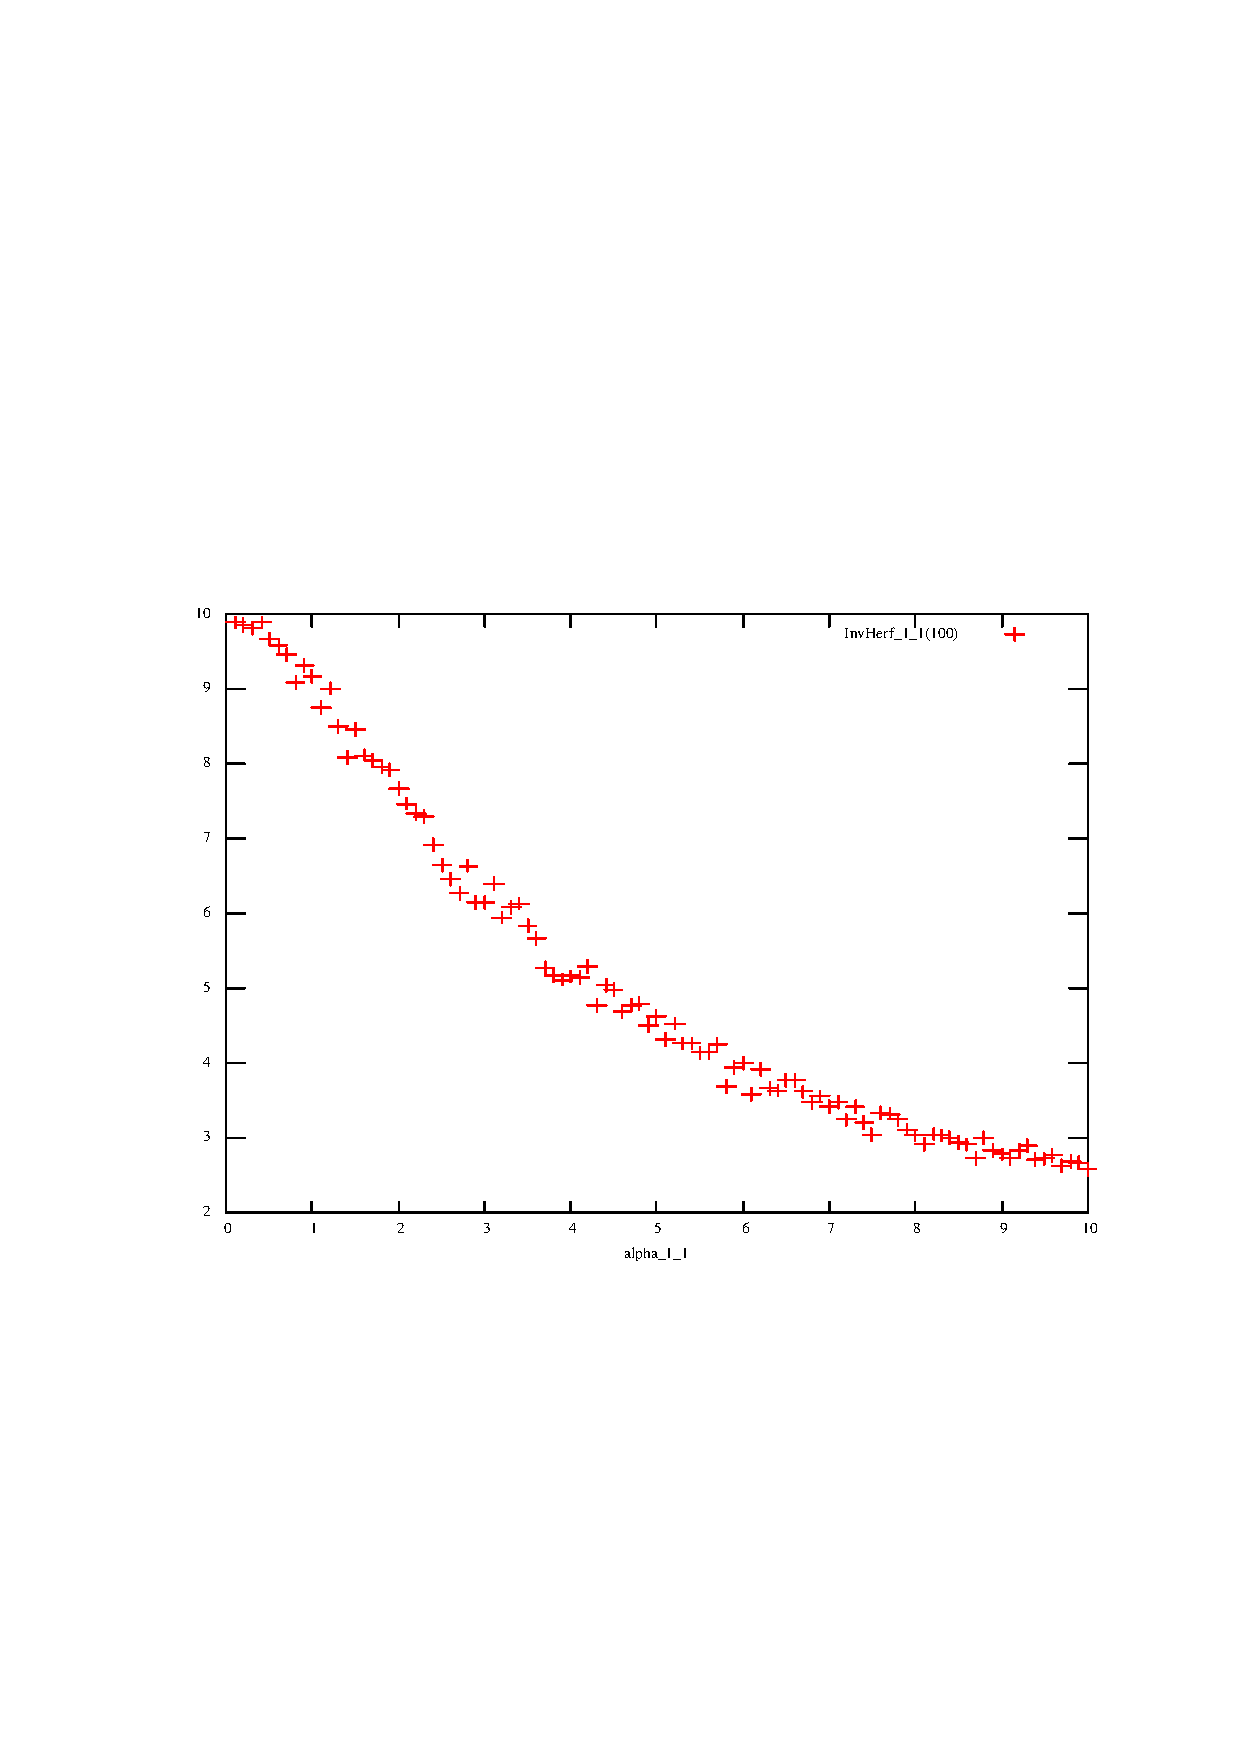
\includegraphics[width=12cm]{alpha.pdf}}
  \caption{\small Values of \lsd{InvHerf} at time 100 expressed as a function of \lsd{alpha}.}.
   \label{fig:alpha}
\end{figure}


This graph shows that lower values of \lsd{alpha} generates higher dispersion, and viceversa. Although the relation is clearly visible, the graph reflects the randomness of the consumers' choice. However, our data contain 100 time steps, each with constant \lsd{alpha} and with (randomly based) different \lsd{InvHerf}. Clearly, getting the average values for each series across all the time steps should provider a clearer relation.

\section{Creating new series}

The Analysis of Results windows can manipulate existing series (as those generated from simulations, but also loaded from files or taken from the current model configuration) to generate new series. Clear the \menu{Series Selected} pressing the button \menu{Clear} and insert all the series for \lsd{InvHerf}. Therefore, there will be 100 series (one for each market) defined over 100 time steps (from 1 to 100), the length of the simulation run.

Press the button \menu{Add Series}. A new window will ask which type of series you want to add to the data set already available. 

\menu{Current model configuration} allows to add to the series available for analysis the data from the current state of the model. These series will result as having a single time step datum available,conventionally indicated with time 0. Any cross section analysis done with these ``singleton'' series will always use the 0 time step, even when used (as in the scatter plot) with other series indicated with other time steps. 

\menu{File(s) of saved results} allow to load a data from a previously saved \LsD simulation. This series will be identical to the data from a just terminated simulation, but for the letter ``F'' added to their label.

\menu{Create series from selected series}. Choose this option and press \menu{Ok}. A new window, reported in figure \ref{fig:createseries}, will ask for a few options.

\begin{figure}[ht]
  \centering
 \fbox{\includegraphics[width=5cm]{createseries.pdf}}
  \caption{\small Options to generate a new series from elaboration of the series in \menu{Series Selected}.}.
   \label{fig:createseries}
\end{figure}

The new series can be generated as one of five statistics: average, sum, maximum, minimum and variance. There are two possible ways to compute the statistics. The first, \menu{Compute over series}, generates a series with the same number of steps as those selected. Each time step of the newly created series will contain the statistics computed on the value for that time step across the selected series. 

The second option, relevant for our purposes, is \menu{Compute over cases}. Choosing this option the system will create a new series with a different virtual time scaling, different from that of the simulation. In effect, this option operate a sort of ``transposition'' of the original data, turning a statistics over time steps in a single element of a new series, whose ``time'' actually correspond to a series. Every ``time step'' for such a series will correspond to one of the series selected: first series will generate the ``time step'' 0 of the new series, second selected series generates time step 1, and so on. For each time of the created series the statistics is computed across all the simulation time steps in which the selected series is defined (in our case from 1 to 100). Choose this option and leave the default choice \lsd{Average}. If desired, you can also set a different label for the new series, whose default value uses the first label and a modifier indicating the statistics used. There is also an entry to associate the new series to a tag, which may be used for searching purposes.

Pressing \menu{Ok} on this button a new series will be generated, placed in the last position of the \menu{Series Available} list box. Notice that the new series has the label and tag defined, and contains as many ``time steps'' as the series originally selected for its creation. It also is attached the name \menu{(created)} to distinguish it from other series.

We now have a series composed, for each of its ``time steps'', of the average values for the different \lsd{InvHerf}. If we generate a time series plot of this series we, in effect, will generate a cross-section plot over all the markets, and using the average value that \lsd{InvHerf} had in each market across all the simulation. This graph is clearly more well-defined that those produced as a scatter plot over a single period, given that the random variability is sensibly smoothed down. However, the time series plot of a created series is, in general, a bad substitute for an actual scatter plot. However, we cannot generate a scatter plot using the existing series \lsd{alpha}'s, since these values are represented as different series, while our average \lsd{InvHerf} is stored as a 100 time steps series. We need therefore to generate another series, using the original \lsd{alpha} and creating a matching \lsd{Avalpha}, following the same way we used to generate the first newly created series, \lsd{AvInvHerf}. 

When the two series are available, both defined over time steps from 0 to 99, we can then generate a scatter plot. Select first the series for \lsd{Avalpha} and then for \lsd{AvInvHerf}. Select the option \menu{XY plot} and \menu{Points} but, differently from the previous scatter plot, select \menu{Time Series}. In fact, the 100 points to generate on the graph must be taken from the series across the same ``time steps''. Press \menu{Plot} and choose between a low-quality, \LsD windowed graph, or a high-quality, external gnuplot graph. The resulting scatter plot will show a much neater relation between the \lsd{alpha} and average \lsd{InvHerf}.


\section{Random events}

The model we have developed so far is still not a proper dynamic model. In fact, it simply draws randomly a new product for each consumer at every time step, ignoring any past event, so that, in effect, generates a series of unrelated random events. In this paragraph we start to modify the model adding a dynamics: past events condition current ones. The objective is to have consumers that generally stick to the currently owned product, and make a purchase only if the currently used product fails in some, unspecified respect. Therefore, the sales observed at any time will depend on the number of consumers per firms in the previous time step, introducing a dynamic content of the model. Before this, however, we need to introduce some new \LsD functions for models' equations

Let's suppose that the model provides consumers with a probability for the product to fail, or need a replacement for whatever cause. To represent in the code a probabilistic event we need two computational structure: a conditional statement and a random event with variable probability. \LsD offers a large number of probability functions. We will use the \code{RND} function which generates a new random value in [0,1] every time it is executed in the code. This function provides a real value with a uniform distribution, that is, the probability of producing a value smaller than a given threshold is the threshold itself: $P(x<X)=X$, with $X \in [0,1]$. Thus, for example, if we execute 1000 times the function \code{RND} we can expect a value smaller than 0.3 about 300 times and a value between 0.3 and 1.0 the remaining 700 times.

This property allows to turn a continuous random uniform function like \code{RND} in a discrete random event (say 0 or 1) whose probabilities can be decided arbitrarily. Consider the following code:

\begin{minipage}[h]{10cm}
\small
\begin{verbatim}
...
if(RND<0.3)
 {/*
 this block of code is executed with 
 30% probability
 */
 }
else
 {
 /*
 this block is executed with the 
 remaining 70% probability
 */ 
 } 
...
 
\end{verbatim}
\normalsize
\end{minipage}

The the program executes the first line of code, it draws a uniform random value; if this value is smaller than 0.3, then executes the first block, and ignores the second. Otherwise, ignores the first block and executes only the code following the \code{else} statement.

Notice the C++ notation for comments: they comprised any text within the \code{/* ... */} symbols. Everything in between is ignored by the compiler. Also, as we have seen also in the case of \code{CYCLE(...)}, the blocks are delimited by \code{ \{ \}}. If the block delimiter are not indicated, the compiler consider the single line following  the \code{if} and \lsd{else} statements as the only component of the blocks.

In our case, the equation for product chosen will then become:


\begin{minipage}[h]{10cm}
\small
\begin{verbatim}

EQUATION("ProductChosen")
/*
Product used by the consumer
*/
 v[2]=... //to place here the probability of the consumer's product to be replaced
 if(RND<v[2])
   v[1]=V("Choose");
 else
   v[1]=VL("ProductChosen",1);

RESULT( v[1])
 
\end{verbatim}
\normalsize
\end{minipage}

The equation needs the probability of the product to breaks down and needing replacement, which we will discuss shortly. If the event ``breaks'' actually occurs, it then calls \lsd{Choose} providing a new product. Otherwise, the equation returns the previous value for \lsd{ProductChosen}. 

The next question is how this equation can obtain the correct value of the probability.

\section{Conditional searches}

As we have seen the equations in \LsD can, most of the times, take the values from other elements of a model without specifying where the elements are contained, that is, in which object. The \code{V(...)} \LsD function returns the most likely copy each equation needs to use. 


However, in some cases the modeller needs to explicitly indicate one of the copies of a multiple-copy element. In our case, we assume that the probability of a product to fail depends on the producer of that specific product. Say that objects \lsd{Firm} contain a parameter, called \lsd{ProbBreak} expressing this probability. In this case, we cannot rely on \LsD to find which firm should provide this parameter when \lsd{ProductChosen} is executed. The reason that any consumer can need to use products through the simulation time, and therefore requires different copies of \lsd{ProbBreak}. Indeed, the very structure of the model tells that we cannot rely on the automatic \LsD identification of a specific copy of \lsd{Firm} for each copy of \lsd{Consumer}. In facts, the two groups of these objects are contained in different ``branches'' of the model, and there is no obvious path leading from one object to another.

To obtain the value of \lsd{ProbBreak} we need therefore to make two steps: firstly, obtain identify a property of the copy of the firm we need; secondly, to identify the object satisfying that particular property. In our case, the property to use is the identification of the product used in the past by the consumer, which can be obtain by the command: \code{v[1]=VL("ProductChosen",1);}. Secondly, we can use a new function returning a specific object, the \LsD function: \code{SEARCH\_CND(''label'', value)}. 

This function scans the model searching for an object, and returns the copy of the object containing an element that meets a condition. The condition is that the copy of the object must have the element \code{label} having the value \code{value}\footnote{If there are many copies meeting the condition, the ``closer'' to the calling object is returned. If no object satisfies the condition, the function returns a conventional value.}.

In our equation the use will be:

\code{cur=SEARCH\_CND(''IdFirm",v[1]);}

whose meaning is: scans the model searching for a copy of the object that contains \lsd{IdFirm} with value equal to \code{v[1]}. The object found is assigned to a temporary pointer, \code{cur}, that is, a C++ variable that stores, instead of numerical values, copies of objects.

Finally, the value of the element \lsd{ProbBreaks} contained in that specific object can be computed:

\code{v[2]=VS(cur, ''ProbBreak'');}

The complete equation's code will then be:


\begin{minipage}[h]{10cm}
\small
\begin{verbatim}

EQUATION("ProductChosen")
/*
Product used by the consumer
*/
 v[1]=VL("ProductChosen",1);
 cur=SEARCH_CND("IdFirm",v[1]);
 v[2]=VS(cur, "ProbBreak");
 if(RND<v[2])
   v[1]=V("Choose");
 else
   v[1]=VL("ProductChosen",1);

RESULT( v[1])
 
\end{verbatim}
\normalsize
\end{minipage}

\section{Endogenizing parameters}

The model represents now consumers that make a new purchase with a probability which is a characteristic of the producer. When they do make a purchase, they choose according to another characteristic of firms, \lsd{Quality}. We may now ask what would happen if the consumers have no information on the quality of products, and choose (when making a purchase) according to probabilities proportional to the market shares of the different sellers.

This assumption amounts to consider consumers as ``trusting'' the market as a whole to suggest the best products, those lasting longer and breaking less frequently. The parameter \lsd{alpha} can then assume a more explicit meaning. The higher this value, the stronger consumers trust the market, giving higher probability to higher market shares. Lower \lsd{alpha} represent, instead, consumers more suspicious of the signals provided by market shares. We can then ask ourselves whether the market is able to funnel the ``correct'' information to consumers, giving higher market shares to products with the lowest probability of breaking down\footnote{This question and the model developed to solve it was posed in Smallwood and Conlisk, 1979, ``Product Quality in Markets where Consumers are Imperfectly Informed'', \textit{Quarterly Journal of Economics}, 93-1. The original authors developed a rather complex system of differential equations, which provides only limited results. The simulation version here developed replicates those results, besides being able to extend the assumptions imposed in the original article.}.

To explore this question we need to modify the model by changing the equation for \lsd{Visibility}:

\begin{minipage}[h]{10cm}
\small
\begin{verbatim}

EQUATION("Visibility")
/*
Evaluate the visibility of the product for the consumer
*/

v[0]=V("alpha");
v[1]=VL("ms",1);
v[2]=pow(v[1],v[0]);
RESULT(v[2] )
 
\end{verbatim}
\normalsize
\end{minipage}

Notice that we are forced to use the past market shares. In fact, consumers makes their decisions at time $t$ before the market shares can be computed, and therefore, using time $t$ market shares for time $t$ decisions would cause a dead-lock error. For this reason we need to edit the variable \lsd{ms} to have 1 lag. 

Compile the model including the new equations for \lsd{ProducChosen} and \lsd{Visibility}. With the new \LsD model program load the previous configuration and add the parameter \lsd{ProbBreak} to the object \lsd{Firm}. Initialize this parameter assigning different probabilities, from 0.19 to the first firm to 0.1 to the last one\footnote{You can use the \menu{Set all} button for this parameter and using the \menu{Increasing} option, starting from 0.19 and steps -0.01.}. We need to make further changes to the configuration. In fact, variables \lsd{ms} and \lsd{ProductChosen} are now used with lagged values. Try to run a simulation without editing these variables: an error message will be issued by the system, signaling the mismatch between the code and the configuration. After the error, close the \LsD model program.

To fix the error we will simply need to edit the variables in the configuration indicating that they need to have a one lag, instead of 0 lags. However, doing this we will need to provide initial values for these variables, that is, assigning initial market shares and initial products used by consumers to be used as time 0 values at the first time step. Though the \LsD initialization functionality is quite flexible, we have now a conceptual problem. In fact, the two initializations need to be consistent: the market shares at time 0 must reflect the number of consumers for each product. The next paragraph discusses how this problem may be easily solved.


\section{Custom initialization: overwriting elements' values}

The initial values for a model sometimes need to be computed in a special manner, ensuring consistency between different series of values. For example, suppose that in our model we want to have that consumers appear, in the beginning of the simulation, to have a uniformly random distribution. The actual number of consumers starting with \lsd{ProductChosen} will likely deviate from the expected value, and we want this deviate to be reflected in the market shares initially assigned to the firms. To obtain this result would be very difficult by using the standard initialization functionalities of \LsD model program\footnote{It may be possible assign 1 to the variable \lsd{ProductChosen} for the first 10\% of the consumers, 2 to the second 10\% and so on, so that to ensure exact 10\% market shares for each firm. However, this approach would need to be repeated if we change the number of consumers in the model.}. Conversely, it would be easy to express the initialization function as the code for standard \LsD variable, but for the fact that the variable needs to be computed only at the very beginning of the simulation run, and never again within the same run.

The content of the equation needs, for each consumer, to choose randomly one \lsd{Firm}, and write the value of its \lsd{IdFirm} onto the variable for \lsd{ProducChosen} of the consumer, making it appear as if the written value was computed at the previous time step, that is, time 0. In the process, the equation needs also to track how many consumers are assigned any given copy of firms, so to be able to compute the market shares. 

The following code represents these computations.

\begin{minipage}[h]{10cm}
\small
\begin{verbatim}

EQUATION("Init")
/*
Initialization function, executed once and then transformed into a parameter
The function 'assigns' randomly one of the firms to each consumer.
In the process computes also the market shares, which must be initialized to 0.
*/
v[2]=0;
CYCLE(cur, "Consumer")
 {
  cur1=RNDDRAWFAIR("Firm");
  v[0]=VS(cur1,"IdFirm");
  WRITELS(cur,"ProductChosen",v[0], t-1);
  INCRS(cur1,"ms",1);
  v[2]++;
 }
CYCLE(cur, "Firm")
  MULTS(cur,"ms",1/v[2]);
  
PARAMETER
RESULT( 1)

\end{verbatim}
\normalsize
\end{minipage}

Let's see how the equation works. First of all, the variable must be located in object \lsd{Root}. This ensures that the variable is executed before anything else in the model at the beginning of a simulation step, since the \LsD Simulation Manager begins from this object to update variables. Moreover, it will be executed only once. In fact, the last command of the code is \code{PARAMETER}. This command transforms the currently executed variable into a parameter, therefore avoiding its code to be executed twice in the same simulation run.

Concerning the operations executed by the equation, they start by setting a C++ temporary variable to 0, which will be used to store the total number of consumers (providing the denominator of the market shares). The equation executes then a cycle throughout all the consumers in the model and all the firms in the model.

In the cycle for consumers, the equation performs the following operations. \code{cur1=RNDDRAWFAIR("Firm")} draws with identical probabilities one of the firms in the model. This command is equivalent to the already seen \code{RNDDRAW(...)}, but for the fact that it needs not to have a distribution of the probabilities specified, and chooses one of the elements with even probabilities. The chosen copy of \lsd{Firm} is returned and stored in the pointer \code{cur1}\footnote{This is another temporary pointer available to modellers. We cannot use the \code{cur} since this pointer is already used in the command for the cycle.}. The \lsd{IdFirm} value from the chosen firms is then read and stored in \code{v[0]}.

The line with the command: \code{WRITELS(cur,"ProductChosen",v[0], t-1);} performs the actual overwriting. This command is a member of the family of \LsD functions \code{WRITE(...)}, which allows to specify which object contains the variable to be written, and the time stamp to be associated to the value. Therefore, this line in the equations writes the value of \code{v[0]} in the variable \code{ProductChosen} contained in the object \code{cur}, and the system will understand as if the value had been computed at time step \code{t-1}. The global variable \code{t} indicates the time step of the simulation, and can be accessed by the modellers but, obviously, must not be modified.

The line \code{INCRS(cur1,"ms",1);} does a similar operation on the variable \lsd{ms}, contained in object \code{cur1}. However, this \LsD function does not writes a specific value, but increases whatever value previously had the variable by the amount specified, in our case 1.

Finally, the cycle terminates by increasing the counter \code{v[2]} by one unit, using the C++ short version equivalent to \code{v[2]=v[2]+1}.

When the cycle through the consumers is terminated, the next cycle scans all the firms in the model. For each of them (stored in \code{cur}, which is now available since it is not used anymore), the line \code{MULTS(cur,"ms",1/v[2]);} performs a similar operation of \code{INCR(...)}, but, instead of adding, multiplies the content of the element by the specified amount, in our case, the inverse of the total number of consumers.

\section{Nested cycles}

Before running the model we'd better make a small change, possibly useless, to the equation for \lsd{Init}. In fact, the code reported above works properly in case we have a configuration including a single market. While we may never be interested in testing configurations using many markets, it is good practice to write equations' code that work safely with any type of numerical initialization.

The code we wrote above makes the two cycles without specifying where the groups of objects for consumers and firms are located. Therefore, the equation for \lsd{Init} will initialize only the first groups (that is, those in the first market). In the hypothetical case there were many markets, the consumers and firms in the markets from the second onward would remain non initialized.

The following code fixes this potential problem.


\begin{minipage}[h]{10cm}
\small
\begin{verbatim}

EQUATION("Init")
/*
Initialization function, executed once and then transformed into a parameter
The function 'assigns' randomly one of the firms to each consumer.
In the process computes also the market shares, which must be initialized to 0.
*/
v[2]=0;
CYCLE(cur3, "Market")
{
 CYCLES(cur3,cur, "Consumer")
 {
  cur1=RNDDRAWFAIRS(cur3,"Firm");
  v[0]=VS(cur1,"IdFirm");
  WRITELS(cur,"ProductChosen",v[0], t-1);
  INCRS(cur1,"ms",1);
  v[2]++;
 }
 CYCLES(cur3,cur, "Firm")
  MULTS(cur,"ms",1/v[2]);
}  
PARAMETER
RESULT( 1)

\end{verbatim}
\normalsize
\end{minipage}

The new equation uses the same code as before, with the only difference that the two cycles for consumers and firms respectively are included within another cycle which scans through all the markets of the model, sequentlly stored in the local pointer \code{cur3}. The two cycles need to be modified so to search the groups of objects from the market pointed to by the \code{cur3} object, using therefore the format \code{CYCLES(pointer, ''label'')}. Also, the command \code{RNDDRAWFAIR(...)} needs to be updated, in order to draw a firm from the set of firms located in the market initialized by the cycle. 

We can now compile and run the model. Load the previous configuration, which should already include the modifications we made before (\lsd{ms} and \lsd{ProductChosen} defined with 1 lag, and parameter \lsd{ProbBreak} defined in objects \lsd{Firm}). Insert the new variable \lsd{Init} in \lsd{Root} and run the model.

\section{Testing the Smallwood and Conlisk (1979) model}
The model is now ready to be tested. The problem we want to investigate is to understand whether a group of consumers unable to evaluate the products on offer, but only to observe their popularity (i.e. market shares), can eventually individuate, collectively, the products with the best (hidden) quality. 

The model represents a number of firms whose quality is implicitly defined by the probability of their products to breaks down, needing replacement, at any time step. Consumers cannot observe this quality, but only the realization of the random event concerning their own currently used product, that is, whether it breaks or not. In case they do need to replace the product, consumers choose randomly among producers with probabilities proportional to $ms_i^\alpha$, where $ms_i$ is the market share of firm $i$ and $\alpha$ is a parameter. We can interpret $\alpha$ as an indicator on the trust of consumers on the market. The higher $\alpha$ the larger probabilities are given to comparatively larger firms, as if consumers ``trusted'' the market to indicate correctly the best producers. Conversely, a smaller $\alpha$ represents markets where consumers tend to ignore market shares as indicators of products' qualities, and choose with similar probabilities all the firms. 

The configuration we prepared contains 10 firms (with decreasing break down probabilities from 19\% to 10\%) and 1,000 consumers. Let's start testing the model for $\alpha=1.0$. Set the number of steps to 1,000 and run the simulation, after having set the market shares to be plotted in the Run Time plot. The result is quite volatile, though the best firm eventually dominates the market and lower quality firms seem to exit the market following the order of their qualities (worse qualities firms exit earlier).

Re-load the configuration and increase the consumers to 10,000. The \lsd{Init} variable ensures that the initialization would work correctly whatever the number of consumers, thus we can directly run the extended simulation, though it will take obviously longer to complete. The results are much clearer, as expected, since the larger number of consumers reduces the random volatility. If you are patient enough, you may still increase the number of consumers to 100,000, whose results are reported in figure \ref{fig:sc}.

\begin{figure}[ht]
  \centering
 \fbox{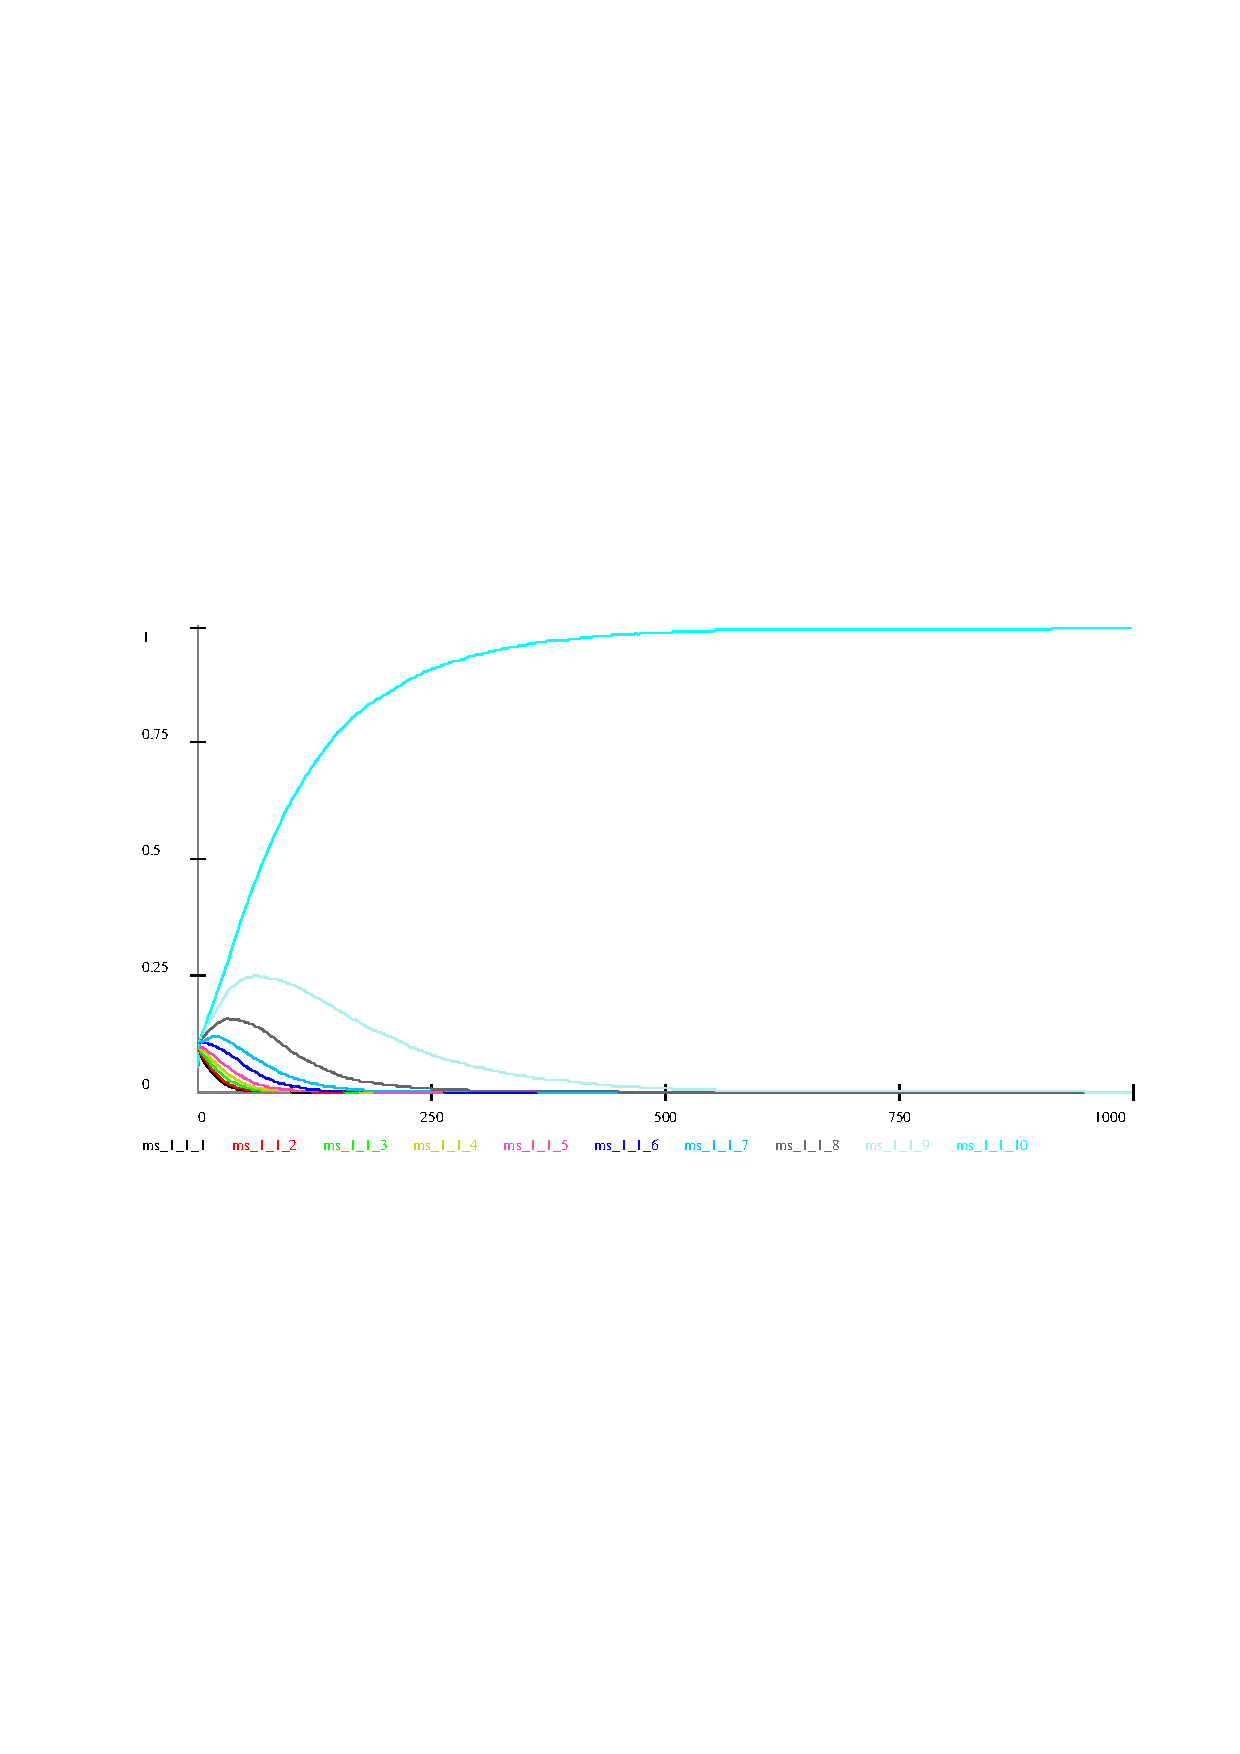
\includegraphics[width=12cm]{sc.pdf}}
  \caption{\small Smallwood and Conlisk model with 100,000 consumers and $\alpha=1.0$. The pattern is identical to that of the replicator dynamics model.}
   \label{fig:sc}
\end{figure}

The results resemble strikingly those produced by the replicator dynamics model, though being generated with a totally different computational structure. In fact, in one case we have the model described at aggregate level, that is, we describe the dynamics of the sales of firms. In the other, this variables' values are obtained as the result of lower level entities, the consumers choosing the products. Moreover, one model is deterministic, and the other is stochastic. Still, they produce identical results, at least with the present configuration.

Re-load a configuration (say that with 10,000 consumers), and test a few simulations using different $\alpha$'s, for example with values 0.7, 0.5, 0.3. As you will observe, all the firms maintain a positive market share, though the high quality ones have consistently higher shares. Moreover, the lower is $\alpha$ is the smaller are the differences between the average share levels of high and low quality firms. Finally, testing the model for $\alpha=0$ generates small, but persistent, differences, even though the consumers choose among firms without any bias.

The model seems, though simple enough, rich of different results that require further investigation. This means that we will need to run many simulations using a large number of consumers, and therefore the speed of execution of a simulation becomes a crucial issue, possibly relevant for the very possibility to exploit the model to its full extent. The reason is that we will need to test many different configurations, comparing the results with different parameterization. If the simulation producing the results we know are relevant takes hours, or even days, this is not a big problem, since we can wait and then having our results. But when we are running a simulation in order to understand the motivations for its results, how certain parameterizations managed to generate certain properties, we cannot wait for hours just for one of many dozens of relevant tests.

In the next paragraph we will introduce new features that allow a simulation model to sensibly increase the speed of computation.




\section{Optimizing simulations: semaphores}

Generally it happens that when we build a working version of a model and begin to make heavy tests on it, we realize that the speed of execution of a simulation run is too slow to allow for an extensive exploration of the relevant parameter space. Though \LsD models are implemented in the possibly fastest language available, the first implementation of a model cannot be focused on minimizing the simulation time. However, once the model has been defined, it is possible to try different versions that, though producing the same results, are far more computationally efficient. 

The present implementation of our example model is highly inefficient, from the computational viewpoint. In fact, we implemented the variable \lsd{Num} in each firm to scan all existing consumers searching for those that are its customers, in effect duplicating the search as many times as many firms are present in the model. A first step to speed up the simulation consists in avoiding this replications. The goal is to implement the model such that, the scanning of all consumers is executed once for each time step, providing all the firms with changes in the number of their customers, \lsd{Num}.

This result can exploit the fact that each consumer either does not make any purchase, or, when it does, ``knows'' both the firm whose product is dropping, and the firm selling its new product. At this moment it is possible to ``tell'' these two firms that they respectively lose a customer and gained a new one.

Suppose that objects \lsd{Firm} contain two parameters, \lsd{Lost} and {Sales}, intended to contain, at each time step, the number of consumers that respectively, dropped the firm and made a purchase from it. Then, we can re-write the equation for \lsd{Choose} as follows:


\begin{minipage}[h]{10cm}
\small
\begin{verbatim}

EQUATION("Choose")
/*
Choose one of the products for the calling consumer
*/

v[1]=VLS(c,"ProductChosen",1);
cur=SEARCH_CND("IdFirm",v[1]);
INCRS(cur,"Lost",1);

cur=RNDDRAW("Firm","Visibility");
v[0]=VS(cur,"IdFirm");
INCRS(cur,"Sales",1);

RESULT(v[0] )

\end{verbatim}
\normalsize
\end{minipage}


The first lines of the equation tell the firm who used to supply the consumer that it lost a consumer. This result is obtained by firstly checking what was, in the previous time step, the \lsd{ProductChosen} of the consumer who activated \lsd{Choose} (that is, object \code{c}). The second line searches for the object containing \lsd{IdFirm} with the same value. Finally, the parameter \lsd{Lost} in that firm is increased of 1.

The next two lines remain as before, providing the new supplier for the consumer. The last line exploits the fact that we have the pointer to the new seller to increase the number of its parameter \lsd{Sales} of 1. 

The modification we made to the equation for \lsd{Choose} allow now to re-write the code for \lsd{Num} as follows:


\begin{minipage}[h]{10cm}
\small
\begin{verbatim}

EQUATION("Num")
/*
Number of customers of the firm
*/

v[0]=VL("Num",1);
v[1]=V("Sales");
v[2]=V("Lost");

v[3]=v[0]+v[1]-v[2];
RESULT(v[3])

\end{verbatim}
\normalsize
\end{minipage}

In fact, we do not need anymore to scan all the consumers to count the ones using the firm's own customers. Knowing the number of previous customers that defected, and the new ones, it is sufficient to adjust the previous values with the balance between these two values.

This implementation avoids firms to use the function \lsd{ComputeSales}, which requires scanning all the consumers, but generates a potential problem, that we need to fix. In fact, \lsd{Sales} and \lsd{Lost} are parameters, they do not change on their own, but are simply overwritten by other equations of the model. This means that one a time step have been completed, the values stored in them remain there. At the subsequent time step the counting of \lsd{Sales} and \lsd{Lost} in each firm will begin from the previous values stored there, messing up the computation. Therefore, we need to reset these parameters to 0 before starting a new counting.

For this purpose we need to introduce a new variable, which ensures that \lsd{Sales} and \lsd{Lost} are set to 0 before any consumer begins to make its purchases. Consider a new variable to be placed in object \lsd{Market}, computed with the following equation:


\begin{minipage}[h]{10cm}
\small
\begin{verbatim}

EQUATION("Trade")
/*
Initialize to 0 all the sales in all firms, 
and then activate all consumers.

*/
CYCLE(cur, "Firm")
 {
  WRITES(cur,"Sales",0);
  WRITES(cur,"Lost",0);
 }
CYCLE(cur, "Consumer")
  VS(cur,"ProductChosen");

RESULT(1 )

\end{verbatim}
\normalsize
\end{minipage}

This variable returns a useless value, which is set to a constant 1. Its code simply sets to 0 the ``trading'' parameters for all the firms, and then asks for the values of variables \lsd{ProductChosen} for all the consumers. Notice that these values are not used: they are simply requested, so that the \LsD Simulation Manager is forced to compute them before \lsd{Trade} can be completed. This variable acts, in effect, as a semaphore: when its value (useless) is computed at time $t$, it means that all firms' parameters have been reset and all consumers completed their purchase.

We can edit now the final version of the \lsd{Num} equation:

\begin{minipage}[h]{10cm}
\small
\begin{verbatim}

EQUATION("Num")
/*
Number of customers of the firm
*/

V("Trade");
v[0]=VL("Num",1);
v[1]=V("Sales");
v[2]=V("Lost");

v[3]=v[0]+v[1]-v[2];
RESULT(v[3])

\end{verbatim}
\normalsize
\end{minipage}

This version of the equation ensures that any copy of \lsd{Num} will begin to execute its relevant code only after \lsd{Trade} completed the execution of its equation's code. That is, \lsd{Trade} acts as a semaphore signaling to \lsd{Num} that the operations on the model required before its code can be correctly executed have actually taken place.

Having used variable \lsd{Num} with a lag, we now need to initialize this variable, as we did with variable \lsd{ms}. This can be easily done editing the variable \lsd{Init}:

\begin{minipage}[h]{10cm}
\small
\begin{verbatim}

EQUATION("Init")
/*
Initialization function, executed once and then transformed into a parameter
The function 'assigns' randomly one of the firms to each consumer.
In the process computes also the market shares, which must be initialized to 0.
*/
v[2]=0;
CYCLE(cur3, "Market")
{
 CYCLES(cur3,cur, "Consumer")
 {
  cur1=RNDDRAWFAIRS(cur3,"Firm");
  v[0]=VS(cur1,"IdFirm");
  WRITELS(cur,"ProductChosen",v[0], t-1);
  INCRS(cur1,"ms",1);
  INCRS(cur1,"Num",1);
  v[2]++;
 }
 CYCLES(cur3,cur, "Firm")
  MULTS(cur,"ms",1/v[2]);
}  
PARAMETER
RESULT( 1)

\end{verbatim}
\normalsize
\end{minipage}


Edit the equation file inserting the \lsd{Trade} variable and modifying \lsd{Choose} and \lsd{Num} as indicated. Run the model and, after loading the configuration, insert the new variable \lsd{Trade} in object \lsd{Market} and the new parameters \lsd{Sales} and \lsd{Lost} in object \lsd{Firm}. Also, edit the definition of variable \lsd{Num}, defining it as having 1 lag. You need to open the \menu{Init. values} window for objects \lsd{Firm} since, containing elements that need an initialization, the system requires the user to initialize them, even though the initial value will be useless.

You can now test the simulation, and, as you will see, will be much faster, specially in the configuration with a large number of consumers. 

After the simulation, reload the configuration and observe the order by which the \LsD Simulation Manager executes the equations. Mark the function \lsd{Choose} to be debugged and set the debugger to be activated at time 1 (\menu{Sim. settings}), and start the simulation. When the debugger interrupts the computation after the first time \lsd{Choose} has been computed, click on button \menu{Print stack}. This will list in the \menu{Log} window the variables currently under computation. The list will start with the first variable in object \lsd{Market} (\lsd{TotalNum}), which triggers the equation for \lsd{Num}, which requests \lsd{Trade}, which triggers \lsd{ProductChosen} (for the first consumer) and, eventually, \lsd{Choose}.

Semaphores are mainly used to implement efficient simulations, replacing the automatic ordering of executions when the model cannot induce the correct order in which the equations need to be executed. This is typically the case when the equations make use of the commands \code{WRITE} or \code{INCR}.

\section{Optimizing simulations: pointer \code{hook}}







\section{\LsD Automatic Documentation}

One of the biggest problems in the use of simulation modelling for scientific research is that the ``proof'' of a simulation results are difficult to provide. Even in the case the author makes available the code for the model and the reader is able to read the language (rare circumstance, at least in social sciences), making sense of the code written by other people is normally extremely difficult, and generally impossible. On the other hand, a verbal or pseudo-code full description of the model is, besides extremely tedious, generally extremely large, taking far more space than the reasonable number of pages available for a paper. And, for even moderately large models, it is likely to be no more readable than the very code. 

The documentation of a model is not only necessary for readers to understand the content of a model, but it is necessary also to the same modeller. In fact, a model is likely to be developed during an extended period, when the modeller stops working on a model and return on it after some time, forgetting the many of the details of the code.

\LsD already simplifies the documentation of the model by dividing the computational part of the model in separated equations. Adding a short comment to each equation's code is a good, and cheap, practice. However, the ``raw'' code of the model is not sufficient to appreciate the full content of the model, mainly for two reasons. Firstly, the code lacks the numerical initialization. Secondly, because, for making sense of the model's working, it is necessary to jump across the code of different variables, while the equations' code, contained in a text file, is necessarily linear.

Having \LsD installed one can load the model and use the \LsD browser to investigate its content. Clicking on the name of a variable one obtain the window shown in figure \ref{fig:variable} (pag. \pageref{fig:variable}). This window can be used also as a documentation tool. The large window in the center can be used to write any text commenting the element. Pressing the button \menu{Auto docum.} the window will be automatically loaded with the comments present in the beginning of the code for the variable, in the equation file. This comment is therefore relevant to be properly maintained, because it will be transferred in all the documentation of the model.

The other two buttons provide the links of the variable (or of the parameter) to the other elements of the model. (\menu{List Vars. using 'X'} shows the list of the variables using \lsd{X} in their code. \menu{List Vars/Pars used in 'X'}) provides, respectively, the list of elements used in the equation for \lsd{X}. Finally, the button \menu{See code} shows the very code for the variable in a new window.





people reading
a paper based on the results of a simulation model are sceptical since it is very
difficult to understand the code written by someone else (and frequently people cannot
even understand their own code after months they have written it). The solution is to
fully document the simulation program, including comments explaining what the code does,
why those initial values have been chosen, and how the elements of a model interact
together. Of course, this is a tedious work, that hardly any modeller does. \LsD tries to
obviate to this problem providing a fully automatic documentation of models providing a
sort of ``manual'' for each model that immediately permits to understand the code and the
working of the model.

Each element of a model (object, variables and parameters) is endowed with a textual
documentation, called \menu{description}, that modellers can use to describe what the
element does. For the modeller it is therefore easy to sketch out in few words for each
element the description of each element. Moreover, \LsD does part of the job
automatically, obviating to the lack of documentation from lazy modellers. Let's see how
\LsD generates the model documentation automatically.

Use menu item \menu{Model/Generate Automatic Descriptions} (and subsequently choosing
\menu{All elements}). The system scans all the model elements and the equations' code and
allocates the resulting information for each and every element. The information differs
for different elements, indicated below:

\begin{itemize}
  \item \textbf{Object}: Include the list of the equations where the name of the object appears (for
  example because the variable creates or destroys the object).
  \item \textbf{Variable}: If exists, copy in the description the comment written by the
  modeller in the very first lines of the code for the equation of the variable. Then
  include the list of variables whose equation contains the name of the variable,
  typically because they use its value.
  \item \textbf{Parameter}: Include the list of variables whose equation contains the name of the parameter,
  because they use its value.
\end{itemize}


 Besides the description, parameters and any other element that need to be
initialised\footnote{We will see in a moment that some variables need to be assigned one
or more values in order to start a simulation. These are the variables that are used with
past values in some equation, and that, therefore, in the very initial steps of the
simulation require user-defined values for ``negative'' time steps.} are also endowed
with a text document describing how the values for the elements have been decided.

The elements' descriptions (and the comments on the initialization) appear in the
options' window of the model elements activated by clicking on the element label in the
Browser (see fig. \ref{fig:variable} at pag. \pageref{fig:variable}). In this window it
is also possible to gather other potentially useful information concerning an element,
like the code of the equation for a variable, or the list of the elements used that can
be used to open these elements' option window.

These \LsD interfaces and texts allow a very easy way to comprehend how even a large
model, with many elements works and is simulated. However, it is also possible to export
all this information in a standard HTML document, called \lsd{Model Report}, that allows
an exploration of the model using a standard HTML browser (i.e. Netscape). To create the
\lsd{model report} for your model use menu item \menu{Browser/Create Report}. The Browser
will open window like the one depicted in fig. \ref{fig:createreport}.

\begin{figure}[ht]
  \centering
 \fbox{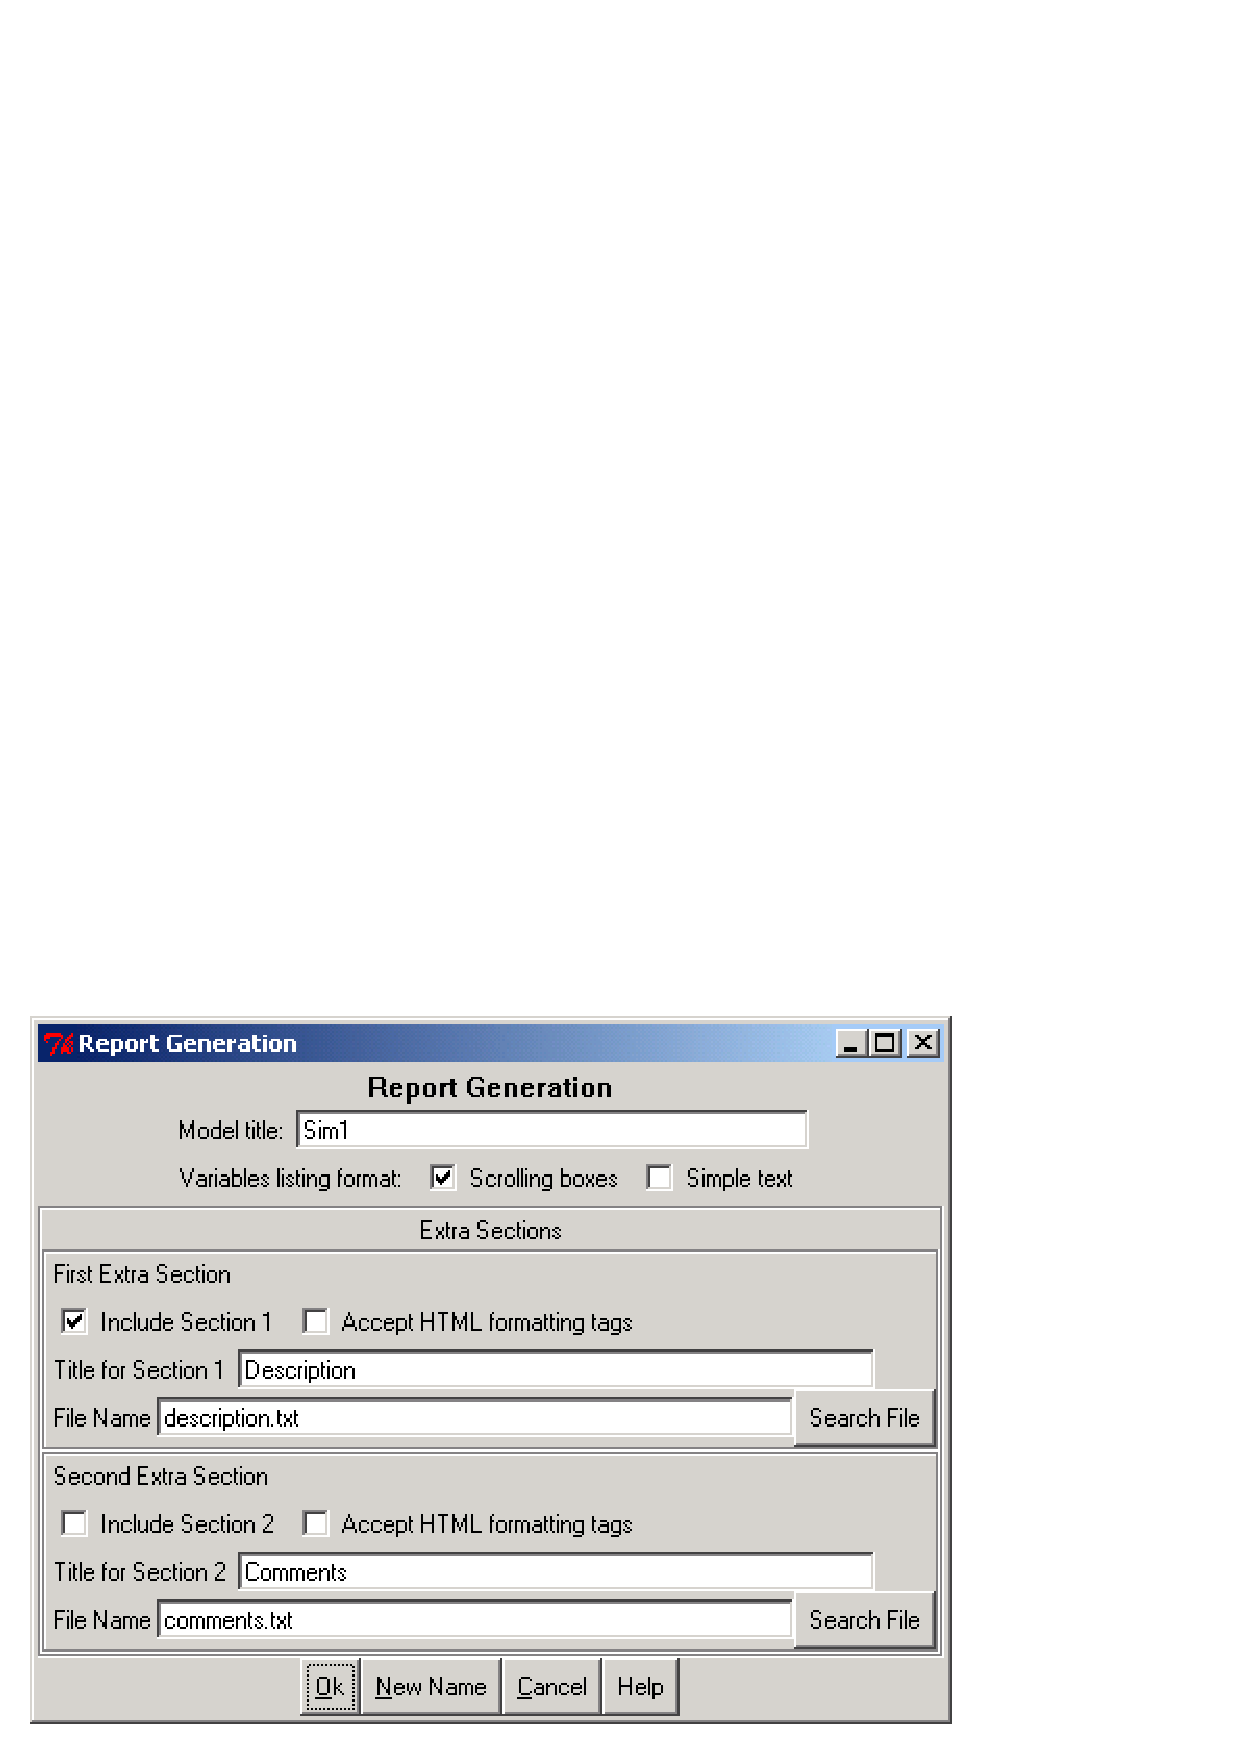
\includegraphics[width=10cm]{createreport.pdf}}
  \caption{Options for the Model Report}
  \label{fig:createreport}
\end{figure}

This window permits to set several options, for example including an external file with
comments on the aim and the results of the model. However, most of times the default
options should suffice.

Pressing \menu{Ok} will start the creation of the report. At the end of the process the
system will start your default web browser to open the report (see the next paragraph for
the use of the \lsd{Model Report}).

Notice that the operation of updating the description of the variables of the model costs
just two clicks of the mouse, and the same applies for the creation of a new report.
Therefore, this document is also a very useful tool for modellers when they are revising
a model editing the equations in order to control for possible conflicts with other
elements of the model.

\section{Using the Model Report}

\begin{figure}[ht]
  \centering
 \fbox{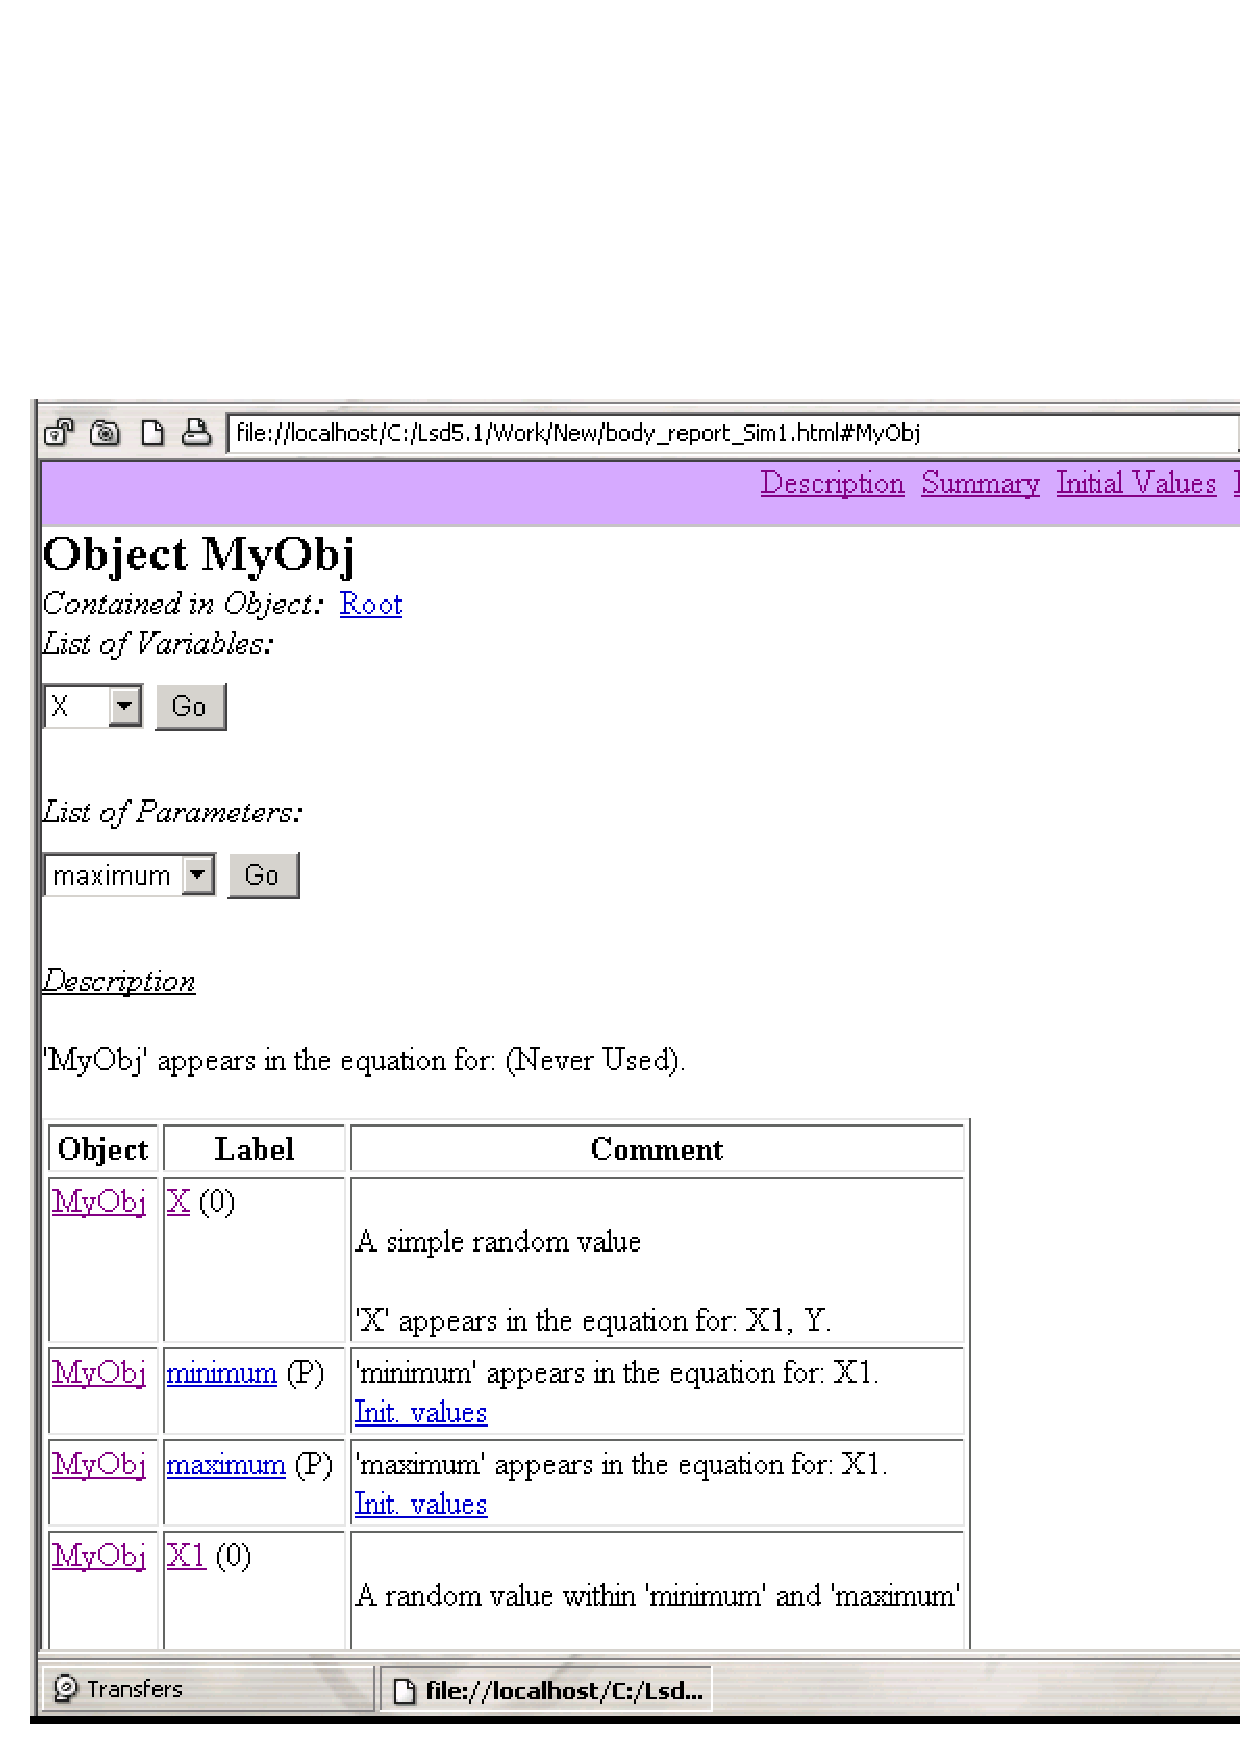
\includegraphics[width=14cm]{report.pdf}}
  \caption{Example of Model Report}
  \label{fig:report}
\end{figure}

Fig. \ref{fig:report} shows a portion of the Model Report for the model developed until
now. The Model Report is opened using the menu item \menu{Help/Model Report}.

The report is composed by four sections reporting different types of information
concerning the elements of the model, each of which is linked to the others with
hyperlinks in order to easily move around the report.

The sections, whose beginning can be reached clicking on the header bar of the document,
contain the following information:
\begin{itemize}
  \item \textbf{Description}: If exists, this section includes a text describing the
  model or any information the modellers considers relevant for the users. Our Model
  Report lacks, for the moment, a description section.
  \item \textbf{Summary}: This section begins with a textual representation of the
  objects forming the model. The labels of the objects can be clicked to reach that
  object's sub-section. Then there are the sub-sections for objects, each formed by a table
  whose columns report:
  \begin{enumerate}
    \item A link to the beginning of the subsection to the same object
    \item The label of the parameters and variables in the object, which is also a link
    to the row of the same element in the section \menu{Detail}.
    \item The text forming the description of the element and, if exists, the text
    commenting the initial values for the element.
  \end{enumerate}

  \item \textbf{Initial Values}: This section begins with a textual representation of the
  objects forming the model. The labels of the objects can be clicked to reach their
  sub-section. Below are listed the sub-sections for the objects, each formed a label of the objects and the number of copies for that object in the
  model, and by a table
  whose columns report (only for parameters and variables requiring initial values):
  \begin{enumerate}
     \item The label of the parameters and variables in the object, which is also a link
    to the row of the same element in the section \menu{Description}.
    \item The values used to initialise the element for a simulation run.
  \end{enumerate}
  \item \textbf{Details}: This section begins also with a textual representation of the
  objects forming the model, which can be clicked to reach their subsection in this section.
  Then there is the list of elements reporting the most detailed information, which
  differ depending on the nature of the elements (any element cited is a link to its cells in the summary section):
\begin{itemize}
  \item \textbf{Objects}: the detailed description of objects report the object that
  contains it; the list of objects contained; the list of variables; and the list of
  parameters.
  \item \textbf{Variables}: the detailed description of variables contain: the label of
  the object that contains it; the list of the variables and parameters used in the
  equation for the variable; the list of the variables whose equation makes use of its
  values; two links to the sub-section for the variable in sections \textbf{Summary} and \textbf{Initial Values}\footnote{This latest link exists only if the variable requires initial values.};
  a link to the beginning of the section \textbf{Summary}. Eventually, this subsection
  contains also the code for the equation of the variable (whose quoted model elements are themselves
  links).
  \item \textbf{Parameters}: the detailed description of parameters includes the link to
  the object containing the parameter; the list to the variables that use the the values
  of the parameter; three links to the sub-section for the parameter in section
  \textbf{Summary}, to its sub-section in section \textbf{Initial Values}, and to the beginning of the
  section \textbf{Summary}.
\end{itemize}


\end{itemize}

The Model Report provides not only all the information concerning the elements of the
model, but also how they are connected, thus providing a useful guide on how, for
example, changing an equation affects the model. Moreover, the report provides readers of
a model with the complete knowledge concerning the model components and how it has been
implemented and initialized, all in a very easy to access manner. Ideally, modellers
presenting the results obtained via simulation could distribute the model report in order
explain readers the inner mechanism of their model, without requiring a full immersion in
the whole code of the model program itself.

The Model Report is extremely useful to be kept updated during the development of the
model. All the descriptions of the model elements are stored in the configuration files,
and therefore loaded and saved together with the configuration itself. When a new
elements is added to the model (i.e. a new variable with its equation) it is enough to
add the description of the new element in the configuration and re-create the Model
Report.

\chapter{Example Models}\label{sec:ex}
\textit{[to be completed]}

\section{Logistic chaotic model}
\textit{[to be completed]}

\section{Spatial market model}
\textit{[to be completed]}

\section{Moving snake model}
\textit{[to be completed]}

\section{Financial market model}
\textit{[to be completed]}

\section{Business plan assessment}
\textit{[to be completed]}

\section{Network externality model}
\textit{[to be completed]}

\section{Nelson and Winter (1982) model}
\textit{[to be completed]}

\section{Lotka Volterra model}
\textit{[to be completed]}

\section{Richardson's dynamic competition}
\textit{[to be completed]}


\section{Percolation model}
\textit{[to be completed]}

\section{Social network model}
\textit{[to be completed]}


\section{Bounded rational demand}
\textit{[to be completed]}


\section{NK fitness landscape}
\textit{[to be completed]}

\part{\LsD Manuals}\label{ch:manuals}

\chapter{LMM interfaces}\label{sec:LMM}

LMM is an auxiliary program supporting the management and constructions of \LsD models. The most frequent activities done using LMM are: identify the model to work with (or create a new one), write the code for the equations of the model, set the options to be passed to the compiler, and run the \LsD model program. LMM is not essential to generate a \LsD model program; any editor can be used to write the equations' file, and the \LsD model program may be generated using a standard makefile. However, LMM simplifies sensibly the usual activities, besides providing other functionalities similar to those provided by an IDE.

\begin{figure}[ht]
  \centering
 \fbox{\includegraphics[width=15cm]{LMM2.pdf}}
  \caption{\LsD Model Manager - LMM}
  \label{fig:LMM2}
\end{figure}

The section documents in detail all the functionalities provided by LMM. The first paragraph below describes the features for the editing environment, while the following describe the menu entries as they appear in the LMM window.


\section{Editor features}

The LMM window contains e menu row, a header, and a main editing window. The header indicates the group and the model currently used by LMM, and the name of the file loaded into the editor.

The LMM contains a standard editor for text files. The editor admits all the standard features concerning selection and movements across the text\footnote{Some of these features depends on the operative system used, and may vary slightly.}, like \menu{Ctrl+arrow} to move the cursor across whole words or paragraphs.

The text for C++ files is colored in blue for strings of characters (recognized by the double-quotes) and green for comments. Moreover, the editor is endowed of with some event-driven functionalities and shortcuts to frequently used commands.

\subsection{Click with the right button of the mouse}
Right-clicking on a text makes a small menu appear, referring to the position of the text cursor where the mouse cursor is located.
\begin{figure}[ht]
  \centering
 \fbox{\includegraphics[width=4cm]{LMM_minimenu.pdf}}
  \caption{Right-clicking on the editor generates a short menu.}
  \label{fig:LMM_minimenu}
\end{figure}

The commands offered by the menu depend on the position of the mouse pointer when the right button have been used. Most of these functions are identical to the equivalent commands accessible through the standard LMM menus. The \menu{Place a break and run gdb} has an additional features. Besides running the gdb debugger on the model, it also places a break in the line indicated by the mouse when right-clicking the text. This will cause the model to be executed and the simulation will be interrupted at the break line.

\subsection{Insert \LsD Script }

\begin{figure}[ht]
  \centering
 \fbox{\includegraphics[width=9cm]{LMM_script.pdf}}
  \caption{Pressing \menu{Ctrl+i} the system automatically inserts one of the most frequently used \LsD commands at the cursor position.}
  \label{fig:LMM_script}
\end{figure}

Pressing the key combination \menu{Ctrl+i} the system will insert in the text at the position of the cursor one of the most frequently used commands for the equations. The resulting window can be operated with the arrows and offers users context-dependent help on the different commands, as well as suggesting default values.

\section{Menu \menu{File}}

The standard menu \menu{File} allows to open, create and save the text files loaded into the LMM editor. 

Unix and MacOS users have also a menu entry allowing to set options for the external programs to be used as terminals (required for the gdb program, see menu entry \menu{Model/gdb Debug}) and the web browser, used for the manual pages.

\section{Menu \menu{Edit}}

The menu \menu{Edit} offers the usual editing functions, plus special functions dedicated to the generation of C++ code. 

\subsection{\menu{Go to line} (\code{Ctrl+l})}

Moves the cursor to the text line indicated by the users. 

\subsection{\menu{Match \{\}} (\code{Ctrl+m})}

When the cursor is position just before a curly bracket \code{\{} or \code{\}}, this command scans the matching bracket, discounting the nested brackets.


\subsection{\menu{Match ()} (\code{Ctrl+p})}
As the command \menu{Match \{\}}, but concerning parentheses.

\subsection{\menu{Insert \{} and \menu{Insert \}} (\code{Ctrl+(} and \code{Ctrl+)}) }

Insert curly brackets in the text, useful for keyboard layouts missing these symbols.

\subsection{\menu{Wrap/Unwrap} (Ctrl+w)}

This command alternates the text between being entirely contained in the horizontal width of the screen, or extending beyond the borders for long line. The wrapping concern only the visibility, and does not affect the actual content of the text file.

\subsection{\menu{TkDiff} }

This entry run a program comparing different text files (supposedly different versions of the same file) highlighting differences between them.

\subsection{\menu{Compare models}}
This command allows to select two files from different models, and launches the \menu{TkDiff} with the two equation files.

\section{Menu \menu{Model}}

This menu contains the commands concerning the model currently loaded in the LMM, if any (otherwise, most of the commands are not active).

\subsection{\menu{Browse Models}}\label{ssec:bromod}

Open the interface to select the model to work on, or to create a new model.

\begin{figure}[ht]
  \centering
 \fbox{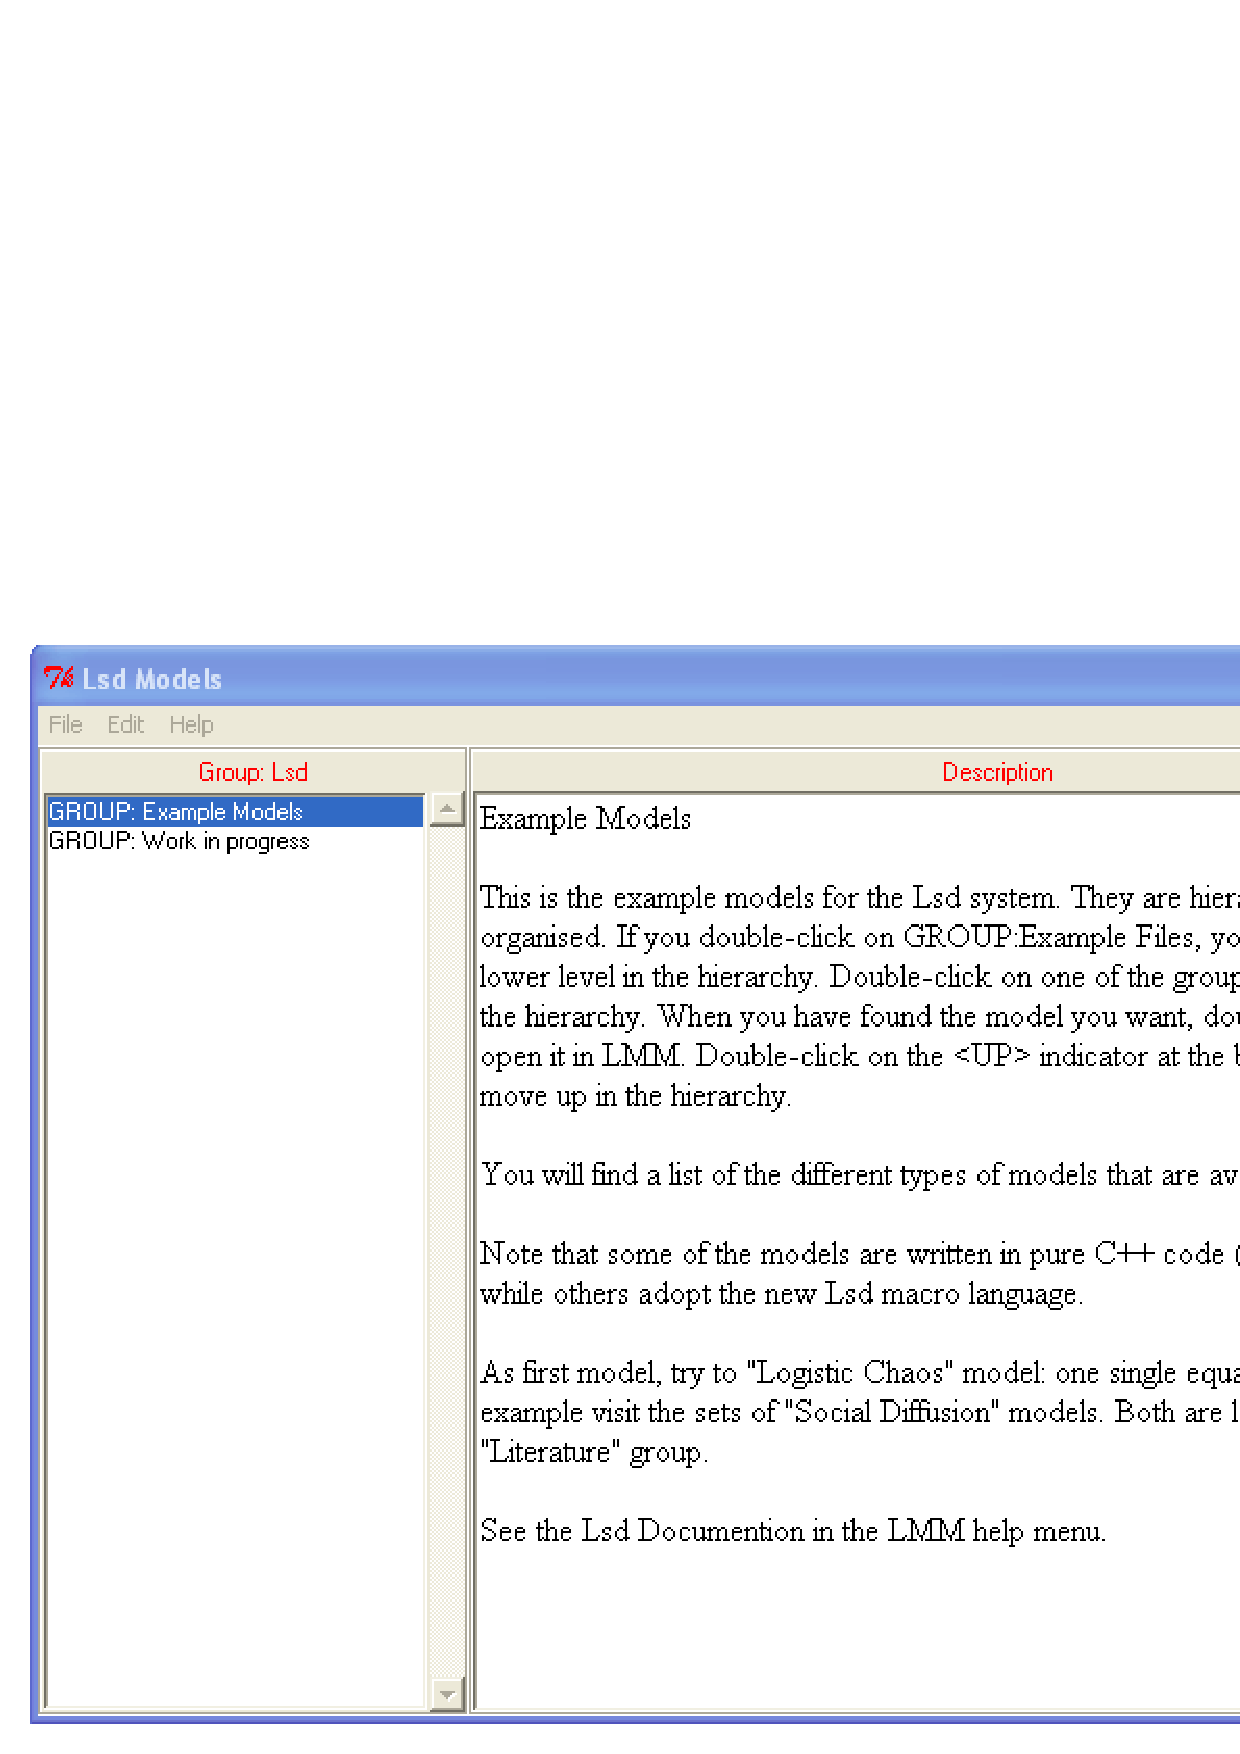
\includegraphics[width=8cm]{browsemodels.pdf}}
  \caption{Menu \menu{Model/Browse Models} activates this interface to select the model to work on, or to create new models.}
  \label{fig:browsemodels}
\end{figure}

The model browser allows to move across the models available in the disk where \LsD is installed. Models are defined within \menu{Group}'s, that is, directories, which can be explored with the arrow keys and pressing \code{Enter}, besides clicking with the mouse. Entry \menu{$<$UP$>$} moves the browser to show the models and groups in the upper directory.

Besides selection, menu \menu{Edit} allows to create a new group or model. From this menu it is also possible to \menu{Copy} a model, which can then be \menu{Paste}d in another or the same group. When creating a model the user is requested to provide a name for the model (a few strings), and the directory name associated to the model. Obviously, the name for the directory must be non-existent and must contain only non special characters (i.e. no spaces, quotes, etc.)

\subsection{\menu{Compile and Run model}}\label{sssec:run}

This entry actually executes three different operations in sequenct. Firstly, it controls whether the text currently shown in LMM has been saved on the disk, comparing the text in the editor with the content of the file. If the text and the file differ, LMM offers the option to save, since the compiler reads the file, not the content of the LMM editor. 
Secondly, after this control LMM generates the \LsD model program concerning the model. This process entails the constructions of the compilation instructions concerning the system code and the model-specific code.  The compilation may fail because the equation file contains illegal code; in this case LMM shows the list of errors as recognized by the compiler.

\begin{figure}[ht]
  \centering
 \fbox{\includegraphics[width=9cm]{comp_err.pdf}}
  \caption{Window showing compilation errors as passed by the compiler. Each line refers to a line of the equation file, indicated by file name (\code{fun\_sd.cpp} in the example) and the line number where the error was recognised.}
  \label{fig:comp_err}
\end{figure}


Each line from the list of errors refers to a line in the equation file (that can be reached with \menu{Ctrl+l}). In figure \ref{fig:comp_err} the compiler found two errors. At line 13 there is a call to command \code{VL(...)} containing only one field and not two, as expected. Moreover, at line 17 the compiler gave up waiting for the semicolon \code{;} ending a command, which actually should have been placed at line 15. This second error is a typical case in which the error occurred not in the line indicated but the preceding one. The window with the list of compilation error can be closed and re-opened using the LMM menu entry  \menu{Menu / Show Compilation Results}.



If the compilation succeeds LMM returns available and the newly compiled \LsD model program is automatically executed.

\subsection{\menu{GDB Debug}}

The gdb debugger is a program allowing users to execute a C++ compiled program line-by-line, normally used to investigate unexpected behaviours of a program. The gdb debugger is a command line program, whose main commands are described in the on-line help of the relative section in the LMM help.

This command runs the command-line GDB debugger loaded with the existing \LsD model program. Notice that this command does not compile the \LsD model program. Therefore, users must be sure to compile and run the model, then close the automatically run instance of the \LsD model program, and only then run gdb.

Notice that for gdb to work properly it is necessary to compile the model with specific options. In LMM you can use the menu entry \menu{Model / Model Compilation Options} and then assigns to the line \code{SWITCH\_CC=-g}.

\subsection{\menu{Show Equation File}}
This command opens in the LMM editor window the equation file used for the model. Users working on a model should always use this command to ensure that the file they are editing is the actual file used to generate the \LsD model program. Obviously, renaming the file opened by the \menu{Show equation} command should never be done, since the saved version is not used for the generation of the \LsD model program.

\subsection{\menu{Show Makefile}}

This command shows the \code{makefile} concerning the loaded model. This command is used only for reading the content of this file, which contains the complete set of instructions required to compile and generate a \LsD model program. This file should not be edited, since the \code{makefile} for any compilation (\menu{Model/Run model}) is re-created any time it is requested. Therefore, changes to one copy of the \code{makefile} have no effect.

To change the compilation options, see the compilation options, in this same menu \menu{Model}.

\subsection{\menu{Show Compilation results}}

This commands shows the error messages generated by the latest attempted compilation, in case it failed. The errors are listed by line numbers on which the compilation identify an error. Normally, the actual error is located just before the line numbers indicated in these error messages. See paragraph \ref{sssec:run} for details.

\subsection{\menu{Show Description}}

This command opens the text file containing the description of the model. Its name must not be modified. The model description is a user-generated text presented at various occasions when the model is observed by users, such as while browsing models and as header of the automatically generated model documentation. Normally, it should contain a summary of the aims and content of the model.

\subsection{\menu{Model Info}}

This command shows the name of the model and its version number (which is associated to the name), allowing the users to modify it, permanently. Also, the user can observe, in read-only, the date of creation and last modification of the model's equations, along the full path of the directory containing it.

\subsection{\menu{System compilation options}}

This command shows the section of the \code{makefile} concerning the options used to compile the \LsD model program. Changes to these options concern the way all the \LsD system code is treated, leaving untouched the way to compile the equations' of the model.

The options are expressed in terms of variables used in the \code{makefile}. These variables concern the location of libraries and files necessary for the compilation, as well as options on the type of executable to generate.

Users may have three reasons to edit these options. In case of installation problems, (i.e. failures to compile because errors not located in the model equations' file) they need to change one or more of the variables indicating the location of the necessary libraries and other files.

The second reason is to generate different types of optimized code. This choice is operated setting to different values the variable \code{SSWITCH\_CC}.

The third reason is to link the executable to an external library. This option can be operated extending the \code{EXTRA\_PAR} content.

\subsection{\menu{Model compilation option}}

This command changes the compilation options specific to the \LsD model program currently loaded in LMM. Three options are permitted: the name of the executable; the name of the equation file to be used; and the optimization options. For the latter use: \code{SWITCH\_CC=-O3} for fastest code and \code{SWITCH\_CC=-g} to use the gdb debugger.


\subsection{\menu{Generate a 'NO WINDOW' makefile}}\label{ssec:nowin}
This command generates within the directory of the model a reduced distribution of the current installation (i.e. the files in directory \code{src}) and of the model file that can be compiled using exclusively pure C++, omitting the graphical libraries 	used for the windows of \LsD model programs. Versions compiled with these options can be compiled on any super-computing machine.

Compiling this reduced version generates a version of the model that is not able to create configurations, but only to execute simulations, even in batch mode. In this latter case at the end of each run the model saves all results in a result \code{.res} file before starting a new one, so that users may leave the program to run and collect later the results (including the \code{.tot} result files).

The NO WINDOW version needs to be compiled at command line, using the associated makefile named \code{makefileNW}. The resulting executable can perform two different types of batch runs. Firstly, it is possible to run many repetitions with the same identical configuration and changing the pseudo random numbers. Secondly, it is possible to use a sequence different configurations.

In both cases it is necessary to prepare the configuration files for the batch runs with a normal version of the \LsD model program. For multiple repetitions of the same configuration just prepare the configuration and specify the number of simulation runs and the initial seed. Save the configuration and run the NO WINDOW \LsD model program from command line as follows:

\begin{verbatim}
$ ./lsd_gnu -f sim.lsd
\end{verbatim} 

This will execute the configuration in file \code{sim.lsd} as many times as indicated in the configurations. The results will be stored in files \code{simX.res} where \code{X} refers to the seed value used for the configuration. Moreover, the final values from each run will be aggregate in a special result file, \code{sim.tot}, where the ``step'' refers to different simulation runs.

The second version of the command has the format:

\begin{verbatim}
$ ./lsd_gnu -f sim -s 1
\end{verbatim} 

(where 1 can be replaced by any positive integer) the program expects to find many configuration files starting from \code{sim1.lsd}, \code{sim2.lsd}, etc. The program will execute all configurations as indicated by the number of repetitions in the very first configuration file, using the increasing indicators. Also in this case the results are saved independently from each tun and collectively in the \code{.tot} file.


\section{Menu \menu{Help}}

This menu provides help pages for LMM and for the general use of \LsD. The three entries in the menu concern help pages on LMM, the list of all the functions available to write \LsD equations, and documentation on \LsD. In particular, a set of slides form a course on \LsD use starting from lessons for beginners in simulation and providing several examples for most \LsD function.


\chapter{\LsD model program interfaces}\label{sec:lsd}

The \LsD model program is a stand-alone executable containing the compiled version of the equation of the model. The \LsD model program allows users to perform every function concerning the model besides changing the equations: create the structure of a model, insert numerical initializations and simulation options, run simulations, analyze the results, etc. 

This section lists all commands provided by the interfaces, which change in accord to the content of models and to the operation currently performed by the user.

\section{Browser window features}
The browser window shows the content of one single type of object in the model and includes all commands necessary to define, modify and exploit a \LsD model program. 

\begin{figure}[ht]
  \centering
 \fbox{\includegraphics[width=6cm]{browser1.pdf}}
  \caption{\small The browser window is the main interface of a \LsD model program. It shows the content of one object and gives access to all commands to the simulation program, like defining a model, initializing its elements, or run a simulation.}
   \label{fig:browser1}
\end{figure}

The left-hand list shows the variables, parameters and functions contained in the object. The right-hand window shows the \textit{descendants}, that is, the objects contained in the object. On the top of these two lists, the browser shows the name of the object shown, and the parent object of this object. Clicking on the descendants the browser moves to show the selected object, while clicking on the parent object the browser moves to show the parent object. It is possible also to use the arrow keys to move across the labels of the objects. The key \menu{u} shows the parent object.

The browser window, besides its menus, allows observe and edit the elements contained in the object, by double-clicking, respectively, on the label of an element in the left-hand list, and on the label of the shown object. 

\subsection{Moving elements}
Within both the list boxes for variables and descending objects it is possible to change the order of elements of the elements using the arrow keys up and down while pressing the control key. The order of the elements normally does not modify the computational content of the model.

\subsection{Options for an element}\label{subsub:opt_ele}

Clicking on an element in the \menu{Variables} list (variables, parameters or functions) the window changes to show the possible options concerning that element, as shown in figure \ref{fig:element_opt}.

The top part of the window is a a header indicating the nature (i.e. variable, function or parameter) and label of the element, besides the object containing it. Double-clicking on the label of the element it is possible to edit its label, or change its nature, for example, turning it from a variable into a parameter. It is also possible to change the position of the element, choosing a different object. Finally, assigning a new empty label to the object the element will be removed from the model.

Below the header there are up to four check boxes. The option \menu{Debug} mark the element to be debugged, meaning that when the simulation is run in debug mode (see below), the simulation will be interrupted showing the state of the model at the very end of the computation of the equation for the element marked as debugged (if any). This option appears only for \lsd{Variables} and \lsd{Functions}.

\begin{figure}[ht]
  \centering
 \fbox{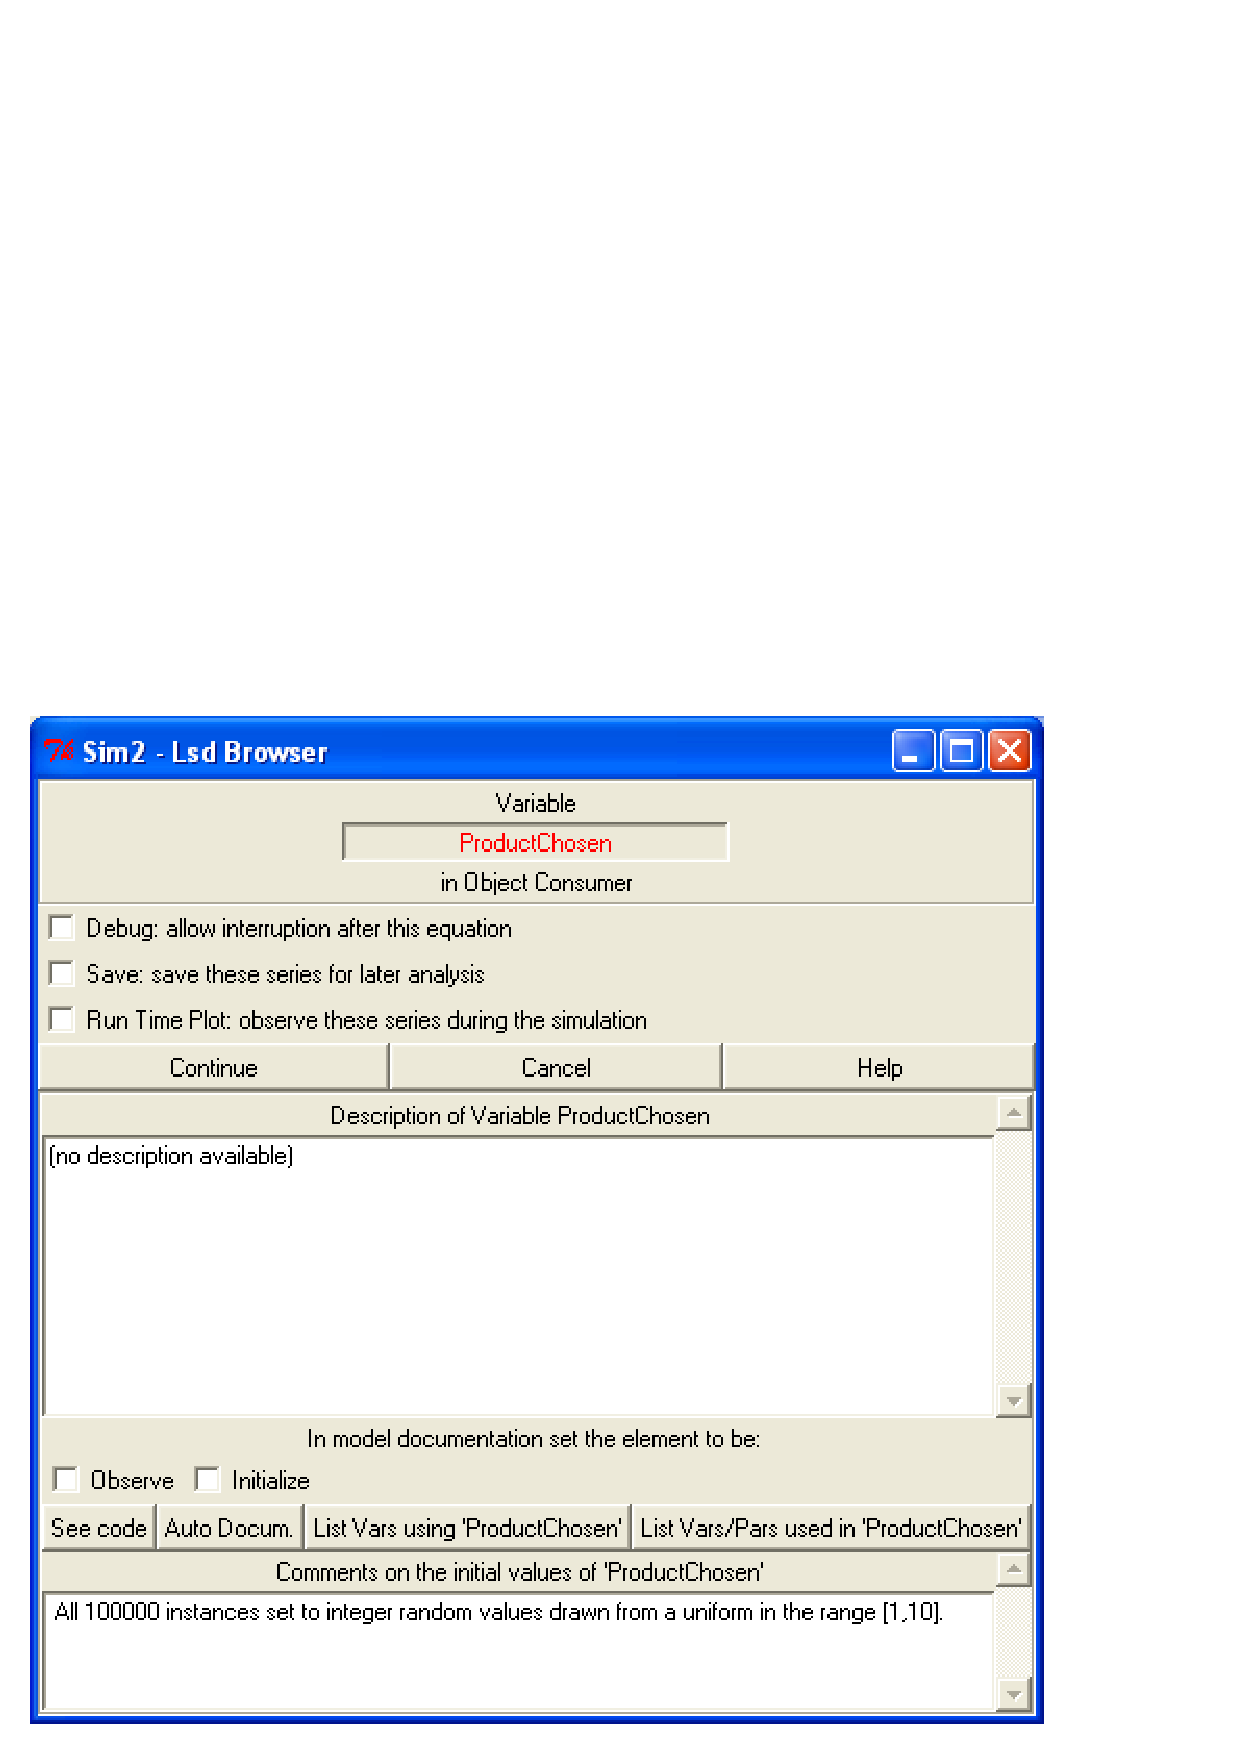
\includegraphics[height=9cm]{element_opt.pdf}}
  \caption{Options for an element, activated by double-clicking or pressing enter on the element's label.}
  \label{fig:element_opt}
\end{figure}



There are several modes to activate the debug mode. Users can set the time step at which the debug mode must be activated (in either the \menu{Simulation Settings} before running a simulation, or the button \menu{Until} in the debug module). Otherwise, users can press button \menu{Debug} in the log window at run time. In any case, when in debug mode, the simulation will be interrupted when the first element marked as being debugged is computed.

Option \menu{Save} impose the system to store every value at each time step to be saved for analysis. Elements with this option unchecked will loose their values as soon as they are no more needed (normally, the subsequent time step of their computation).

Option \menu{Save in a separate files each series} will store the values for this element in a separate file labeled after its name and a code referring to its position in the model structure.

Option \menu{Run Time Plot} set the element's values to appear in the dynamic Run Time plot graphical representation while running the simulation.

Button \menu{Continue} confirm any change made to the options and return to the browser.

Button \menu{Cancel} reject any change made to the options and return to the browser.

Button \menu{Help} opens the help page for this window.

The text window entitled \menu{Description of the ...} can be filled with any text documenting the element, supposedly explaining its meaning to readers of the model documentation. See the button \menu{Auto Docum.} below.

The option \menu{Observe} allows to include the elements whose results should be relevant to observe my the model users.

The option \menu{Initialize} is present only for the elements admitting initial values, that is parameters or other elements defined as being used with a lag. This option allows to include the element within the set of elements whose initialization is relevant for the model.

The button \menu{See code} is present only for variables and functions. Press this button generates a new window containing the code of the equation for the element.

Button \menu{Auto Docum.} fills the text for the description of the element. The text inserted depends on the nature of the element. If it is a \lsd{Variable} or a \lsd{Function}, it is the text contained in the first lines of comment present in the equations' code immediately after the beginning of the equation's code. This comment is supposed to contain the relevant description for the element. For any kind of element, including parameter, the text is completed with the list of elements (if any) whose equations contains the element shown. This information is assumed to be relevant as documentation to understand which part of the model is affected by this element, but does not affect the model results

Button \menu{List of vars. using '...'} generates a list of the elements whose equations make use of this element. This list can be clicked to move the browser to the elements selected.


Button \menu{List of vars./pars. used in '...'} generates a list of the elements appear in the equation's code code for the element. This button appear only for variables and functions.

The final text window appears only for elements that may be initialized, like parameters and other elements declared with a lag. The text contained here describes how the element has been initialized. By default, the initialization functions fill automatically this window.


\subsection{Objects' options}\label{ssec:objopt}
Clicking on the label of the object in the main  \LsD browser (figure \ref{fig:obj_opt}) it is possible to change the name of the object or, assigning an empty label, to delete the object from the model. Removing the object removes also all the descending objects. 

\begin{figure}[ht]
  \centering
 \fbox{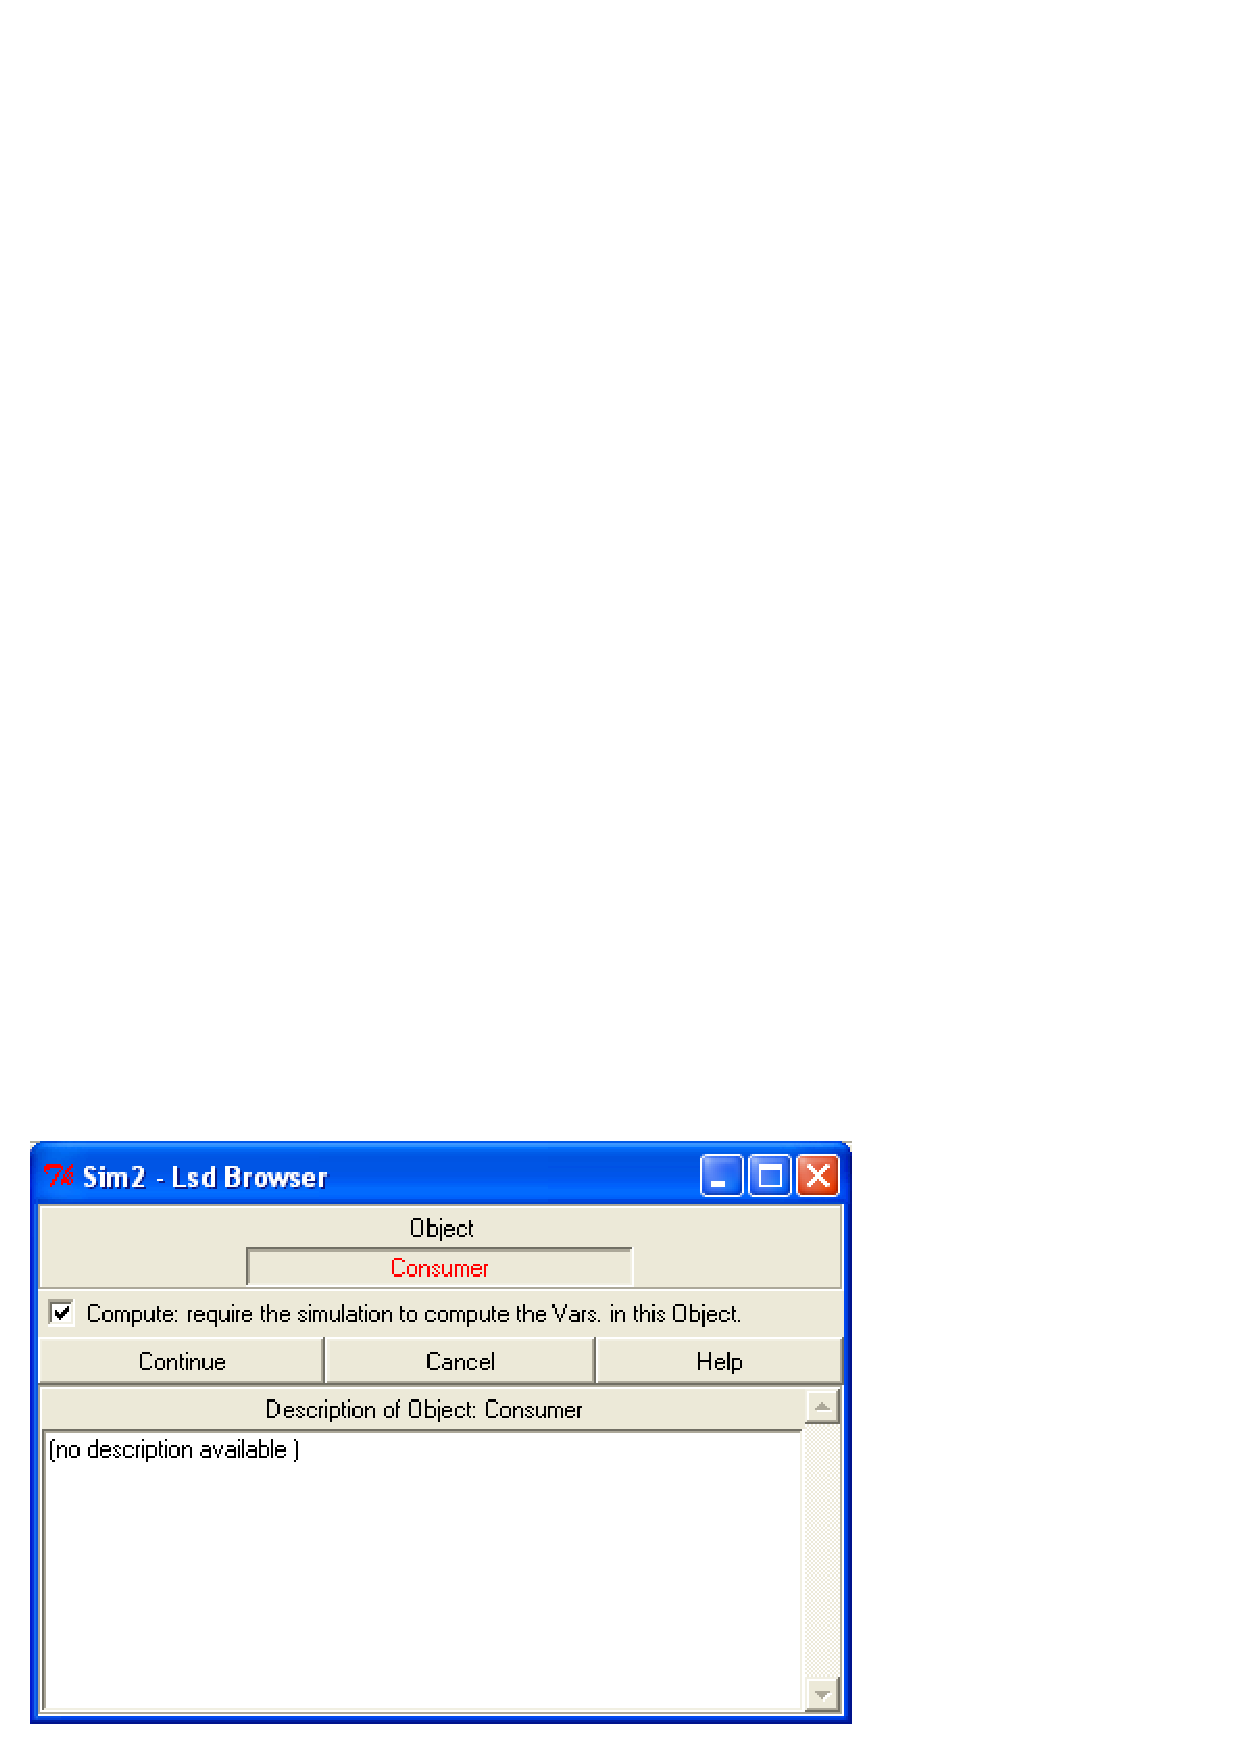
\includegraphics[height=4cm]{obj_opt.pdf}}
  \caption{Options for an object, activated by pressing the label of the object shown by the \LsD browser.}
  \label{fig:obj_opt}
\end{figure}


The check box \menu{Compute} (set on by default) allows the \LsD simulation manager to visit the object at every time step and compute the variables contained in the object. Checking off this option prevents the \LsD simulation manager to update automatically the variables contained in the objects, including also the variables in the objects contained in the object. As a consequence, the simulation will be faster, but the modeller must ensure that, if any variable is contained in the object or its descendants, they are updated because explicitly triggered by the code for other equations. Moreover, any element contained in the objects not visited by the \LsD simulation manager will not appear in the elements saved for analysis of results, even though they have been marked to do so.

The text section in the option window defined as \menu{Description of object ...} can contain any text describing the object, which will be used for the documentation of the model.



\section{Menu \menu{File}}

The model contained in a \LsD model program can be stored in a file to be later reloaded. These files, called configuration files, store every relevant information containing the model. Loading a configuration file restore the \LsD model program in the same conditions as when the file had been saved (aside possible simulation results, if any).

The menu \menu{File} concerns the opening and saving of configuration files. Note the \menu{Re-load}, with its shortcut \menu{Ctrl+w}. This command loads the configuration with the same name as that currently loaded into the \LsD browser. This is mostly used at the end of a simulation run to reload the configuration and run another simulation, possibly after editing the initial values or other settings.


\section{Menu \menu{Model}}

This menu allows to modify the structure of the model, for example, adding elements to the object shown in the browser. This menu should be used only when building a model;  data and simulation options are controlled by the other menus.

\subsection{\menu{Add a variable} (\menu{Ctrl+v})}

Add a variable to the object shown in the browser (figure \ref{fig:new_var}). Variables are elements associated to an equation, which is used at each time step to compute a value for the variable. 

\begin{figure}[ht]
  \centering
 \fbox{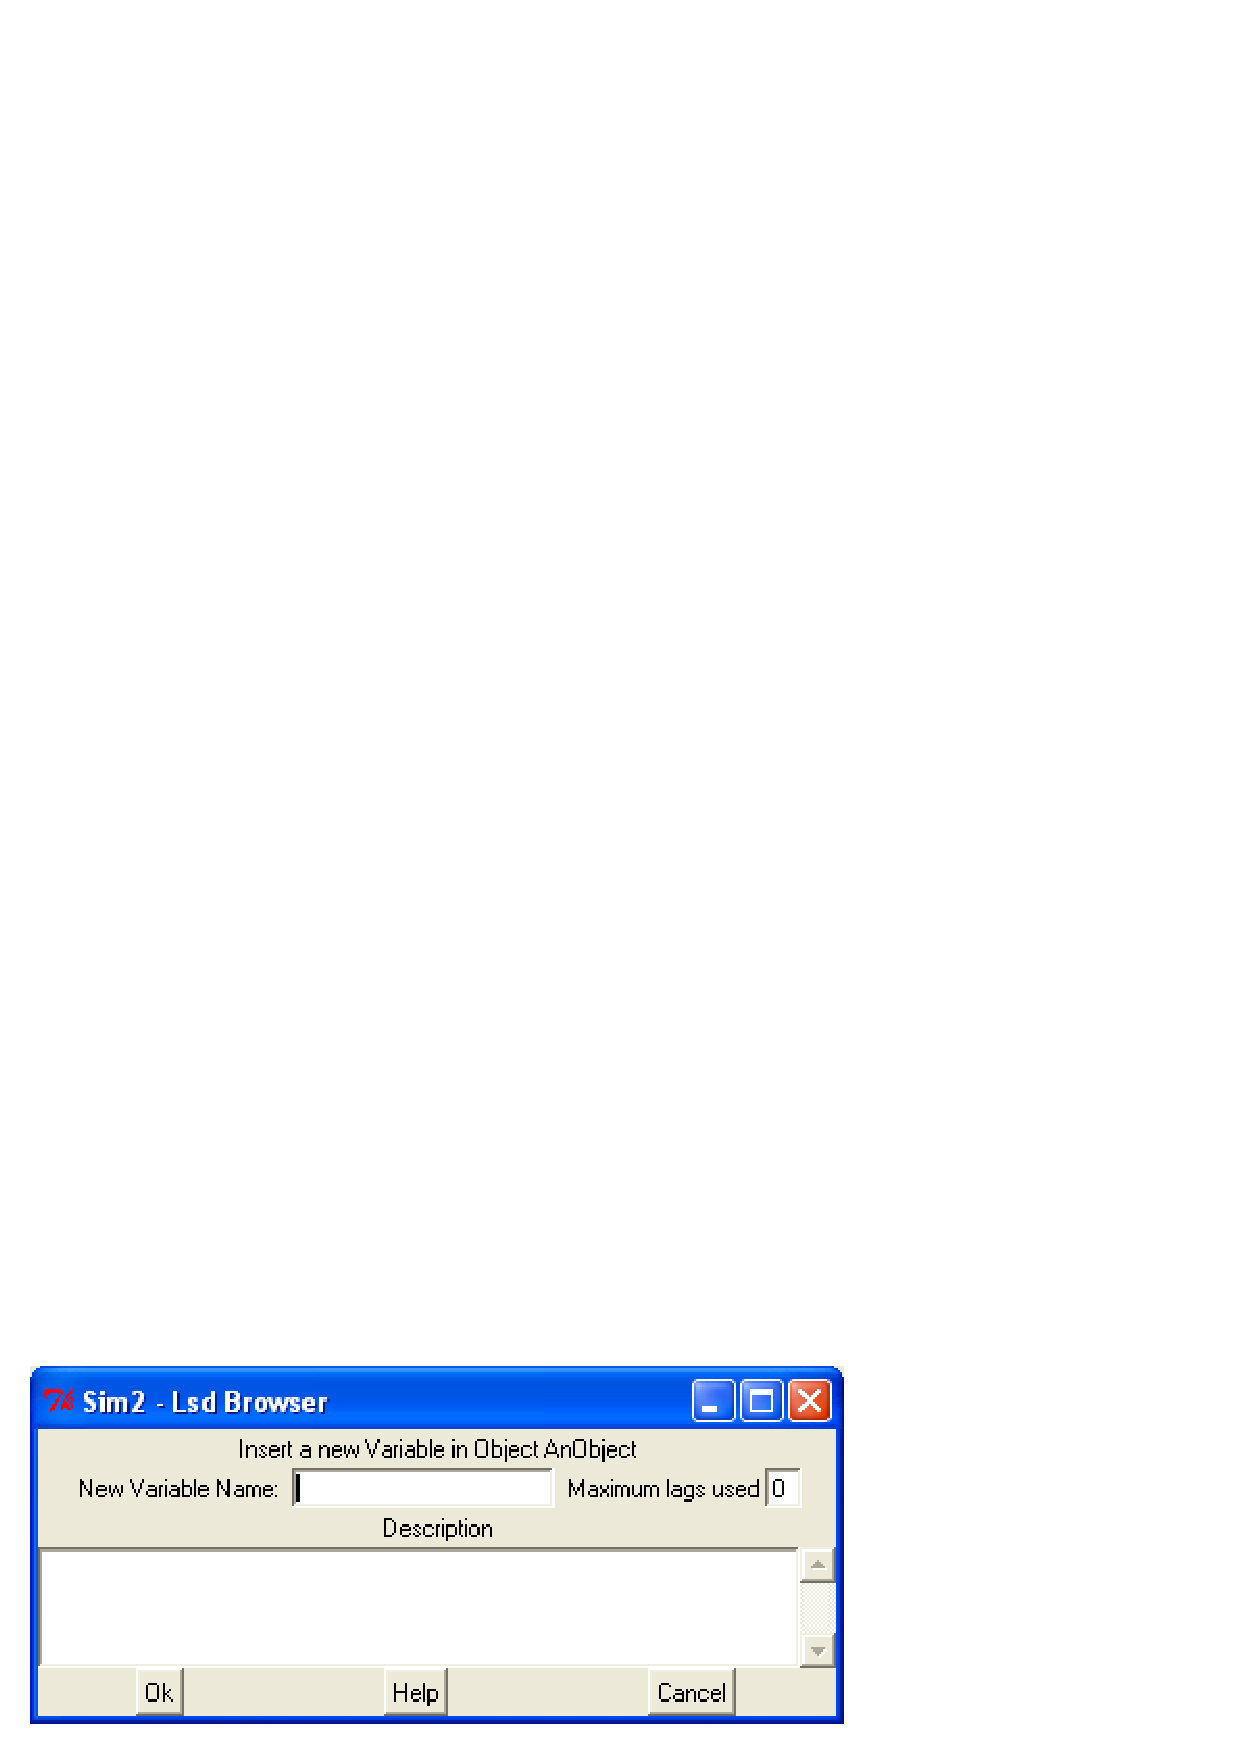
\includegraphics[height=3cm]{new_var.pdf}}
  \caption{Adding a new variable to an object requires the label of the variable and a number of lags.}
  \label{fig:new_var}
\end{figure}

New variables are inserted by assigning a label and a number of lags. The label must be a text string without special characters, as spaces, quotes, etc., and must not be used elsewhere in the model. The label must match the variable's equation headers, and the matching is case-sensitive (i.e. \lsd{X} is different from \lsd{x}). When the variable is created it is not necessary that the corresponding equation already exist, but the model can be successfully executed only if the \LsD model program is compiled with the equations for all the variables and functions declared in the configuration.

The number of lags must be the highest lag by which the new variable is used in some equation of the model. If, for example, the variable value is never requested by other equations with its past values, then the number of lags can be zero. Conversely, if the model includes an equation where the new variable must provide its past value (at time $t-1$), then, the number of lags must be 1. If it is requested with its values at time $t-k$, then the number of lags must be $k$.

Notice that variables declared with lags must be provided with initial data, that is, the values to be used in the earliest time steps as past values, which would refer to a negative time.

If a variable is declared with a number of lags smaller than those used in the model's equations, the simulation run will be interrupted and generate an error. In these cases, it is possible to edit the variable's definition accessing the variable's options, and change its nature by clicking on the variable labels. 

When inserting a new variable it is possible to provide a textual description of the variable, although this information is generally provided automatically using the text inserted in the equation's code (see the section on elements' options \ref{subsub:opt_ele}). The elements' descriptions are used for the various forms of documentation of a model.


\subsection{\menu{Add a parameter} (\menu{Ctrl+p})}

Add a parameter to the object shown in the browser. Parameters are elements that do not change value of their own accord during a simulation run, although they can be written over by the code of some equation. Parameters can be saved as sequences of values, to be used in the analysis of results, if this makes sense.

The label of a parameter must be a string without special characters. As for variables, a textual description may be provided.

\subsection{\menu{Add a function} (\menu{Ctrl+n})}

Add a function to the object shown in the browser. Functions are like variables, but for a crucial difference. Both functions and variables are associated to equations that compute their values. The difference is that variables are computed always once, and only once, at each time step, and the system ensures that this happens under every possible circumstance. Instead, functions are computed (i.e. their equation is executed) only, and every time, the function's value is requested. Therefore, a function may have its equation computed several times or never within a time step, depending on the calls by other equations, while a variable has its equation executed once and only once at each time step. In a sense, variables are used to time-driven dynamics, taking new values in synch at each time step, while functions are used for event-driven dynamics, when a computation is triggered by other events. In \LsD models the two approaches are normally used in the same model, using the most appropriate for each part of the model.

Functions can be declared, like variables, with lags. However, the ``past'' values of functions do not refer to the number of previous time steps, as variables, but to the number of previous activations of the function. Variables cannot be saved, as they do not produce meaningful time series.

\subsection{\menu{Add a descending Obj.} (\menu{Ctrl+d})}

Add a new type of object to the object shown in the browser. The new (empty) object will be located as contained in the object shown by the browser. The label of the object must be a string without special characters.

\subsection{\menu{Insert a new parent} }

Insert a new object above the currently shown object, so that the latter will have the new object as parent. For example, if object \lsd{A} contains object \lsd{B}, and this command is used when the browser shows \lsd{B}, the new object will be located as contained in \lsd{A} and will contain \lsd{B}.

\subsection{\menu{Change obj. Name} }
Modify the label of the object shown by the browser. Inserting an empty string delete the object from the model.

\subsection{\menu{Set equation file label} }

Define the file name of the equation file. This field is automatically filled by LMM when generating the \LsD model program, and it is subequently stored in the configuration file, normally transmitted in different configuration files without need for the user to change it. The file name is used only for presentation purposes, in that the \LsD model program cannot modify the equations of the model. The equation file is used to generate the automatic documentation.

\subsection{\menu{Ignore equation file controls} }

A copy of the equation file is contained in the configuration file, and it may be compared with the actual equation file of the model. If this option is not checked, the \LsD model program compares the equation file of a configuration with that of the actual equation file. If the two files differ, a warning is issued. 

\subsection{\menu{Upload equation file} }

Store in the current configuration the equation file present in the model directory. This file is used only for presentation and control, not for actual computations.


\subsection{\menu{Offload the equation file} }

Generate a new file exporting the part of the configuration containing the equation file. This command is used to transfer a model, by sending only the configuration file and, with this command, re-creating the equation file.

\subsection{\menu{Compare eq. files} }

Generate a temporary file with the equation file stored in the configuration file, and compare (using TkDiff) this file with the actual equation file present in the model directory. TkDiff highlghts the difference in two text files, smartly managing lightly modified texts.

\subsection{\menu{Generate automatic documentation} }

Any element in a \LsD model is associated to a text that the modeller can use to document that element. This text is then used for the model report and, in any case, store in the configuration file for potential users of the model. 

However most of the descriptions' content can be automatically derived, or copied from previously written text. Using this command the system deletes the description of the elements and replace them with the automatically generated ones.

For variables and functions the description is copied from the earliest commented lines located in the equation file, just under the line stating the beginning of the equation for that element. Normally, this is the very only text that modellers need to write (and keep updated) concerning an element.

For objects and parameters the system reports the list of the elements whose equations include the label of the object or parameter. This last part of the description is optional, so that users may update only the text associated to variables and functions.

\subsection{\menu{Create report} }

Generate automatically the \LsD model report, a documentation of the model in HTML format that links together all the information on the model elements and their interactions. See the paragraph on menu item \menu{Help/Model report} for more details.

\begin{figure}[ht]
  \centering
 \fbox{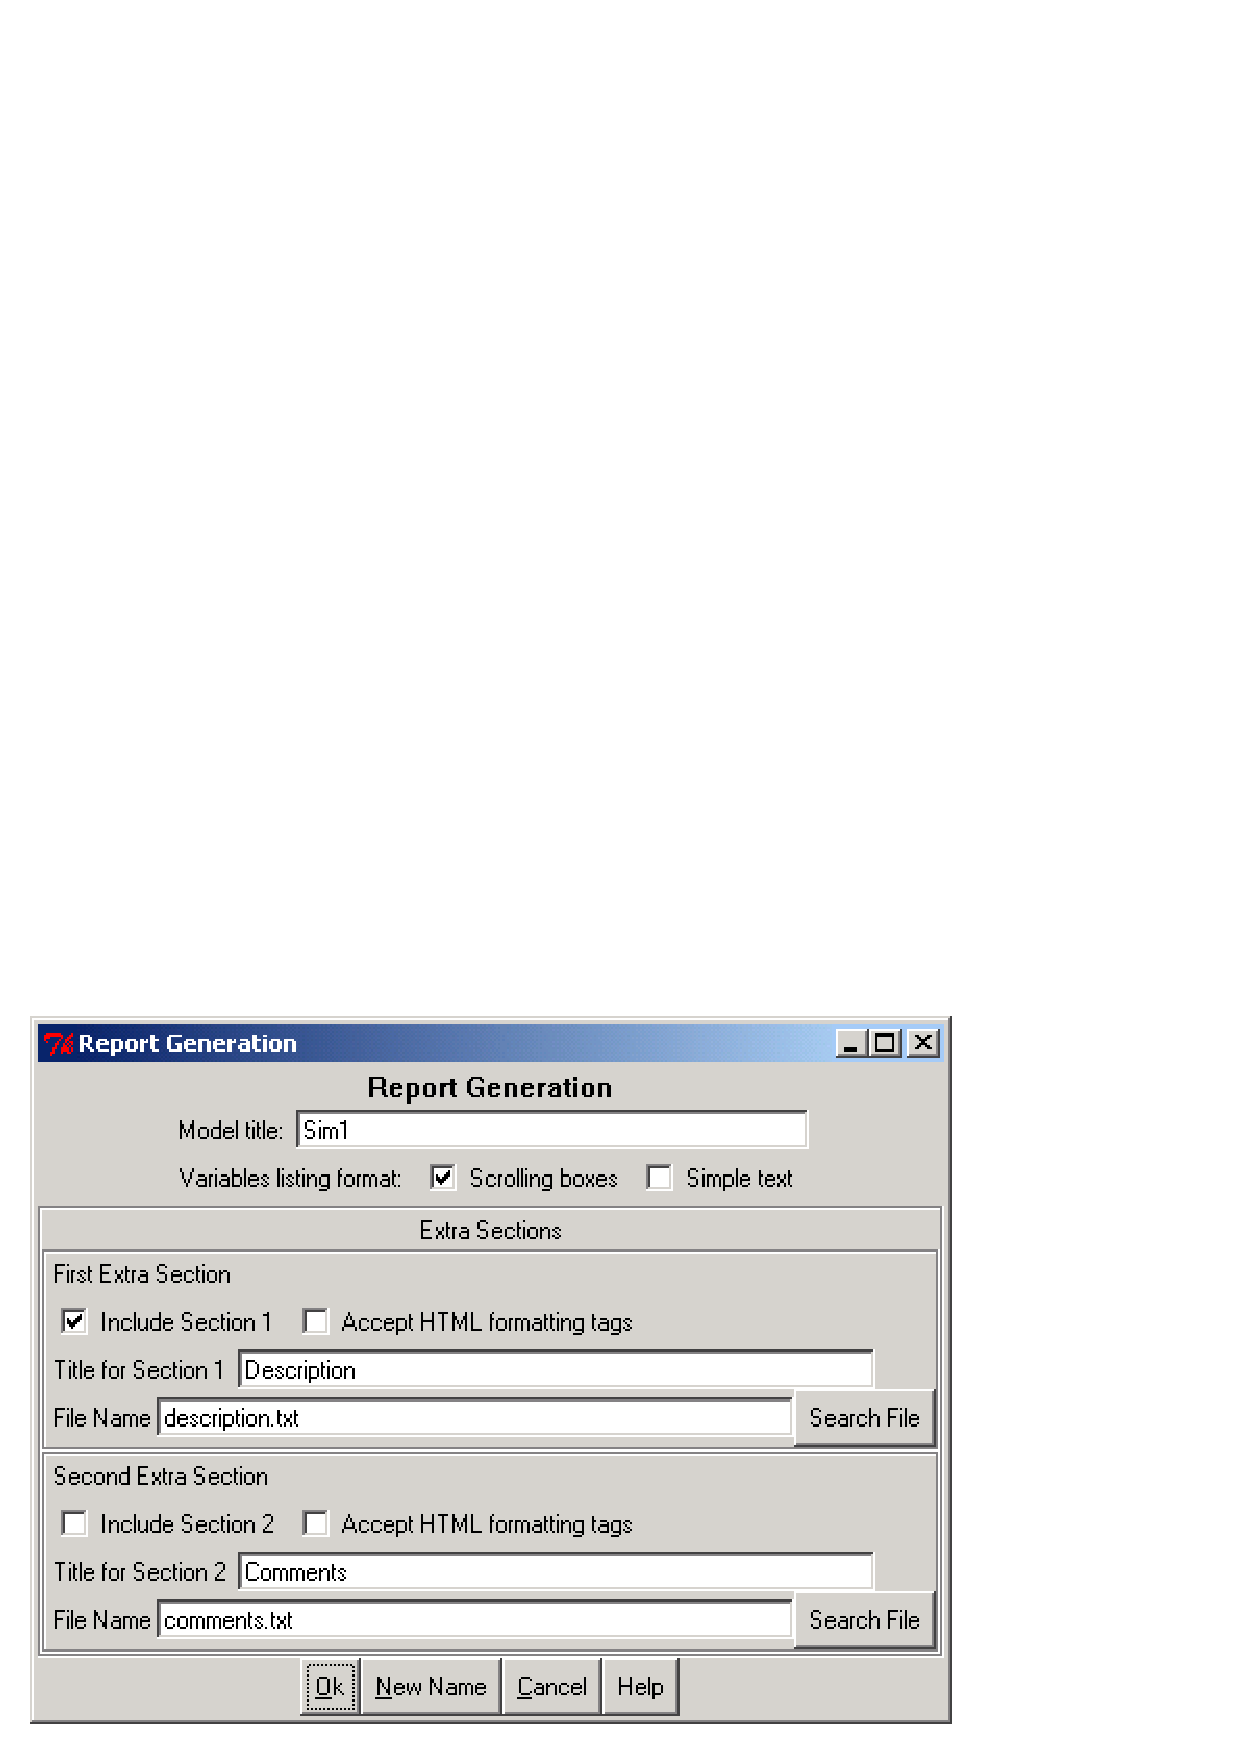
\includegraphics[width=7cm]{createreport.pdf}}
  \caption{Creating a \LsD report the user can set a few options concerning the report naming and additional files to insert in the report.}
  \label{fig:create_report}
\end{figure}

The report is given by default the title, as well as the file name, of the the configuration currently loaded. Users can choose different titles and different file names to store the report. The report contains several lists of elements. When creating the report it is possible to choose between lists presented as pull-down menus or simple lists of links. Moreover, the report normally includes an introductory text, and the user can choose whether to use one, two, or no file to copy the text from.



\subsection{\menu{Create LaTex report} }

This commands generates a report in Latex format. These reports contain the same information as the \LsD reports, but for the sets of initial values used. Latex reports are composed by sets of tables in Latex format containing the list of elements for each object, and the documentation for each element. Latex report should be edited as appropriate, and then inserted in a Latex document.




\subsection{\menu{Find an element of the model} (\menu{Ctrl+f})}

Search the model with an element with the specified label. The browser will show the object containing the element.



\section{Menu \menu{Data}}

This menu contains the commands related to the numerical content of the model. The data concern the initialization of the model before a simulation run, the analysis of results produced by a simulation run, and the observation of the current state of the model.

There are two types of data necessary to execute a simulation run and that can potentially affect the results. First, the user needs to specify the number of each type of object. Second, numerical values must be assigned to all the elements requiring a value at the start of a simulation run, i.e. at \code{t=1}: parameters, lagged values for variables and functions.

Below we list the different commands present in the menu and describe in detail the use of the modules triggered by those commands

\subsection{\menu{Set number of objects} (\menu{Ctrl+o})}

This command allows to define the number of objects in the model. There are two options available. The first option (\menu{All types of objects}) allows to determine the number of objects for the whole model structure. This command permits to customize potentially complex model structures, such as diverse numbers of objects for different branches of the model. For example, in a model with objects \lsd{Market} containing sets of objects \lsd{Firm}, allow to define many \lsd{Market}'s, each containing a different number of \lsd{Firm}'s.

The second option (\menu{Only current type of objects}), allows to determine only the number for all the groups of objects of the same types as the objects shown in the browser. This second option is obviously more limited, but it is much faster to implement, and it is the only practical way to define very large number of objects whose sheer number would crash the initialization interfaces.

Notice that for very specialized initialization there is a third way to solve the problem of complex initialization. In many models it is possible to devote a \LsD variable to implement the initialization.

See the section on \ref{ssec:numobj} (p. \pageref{ssec:numobj})  for the use of the module on setting the number of objects.


\subsection{\menu{Init. values} (\menu{Ctrl+i})}


The initial values necessary to start a simulation are the values of parameters and lagged variables (and functions). Lagged elements require at least one value because they are requested in the equations with a lag, that is, for example, with their value at $t-1$. At the very first step of the simulation ($t=1$) it is obviously not available any value for previous (non-existent) step and therefore the system needs the modeler to provide these values. If a variable or a function is used with more than one lag, then the modeler must provide as many values as the lags. 

Using this command the user activated a module of the \LsD model program allowing to set the initial values for all the necessary elements contained in all the copies of one object type. See paragraph \ref{ssec:initval} (p. \pageref{ssec:initval}).

\subsection{\menu{Sensitivity (parallel) }\label{sssec:senspar}}

The goal of sensitivity analysis is to replicate a given simulation run (i.e. a model with the same setting) many times, where each simulation run differs from the others for the values of of one or more elements to initialize, including the random number generator.

There are two types of sensitivity analysis: parallel and sequential. In the first case the tree of a model is multiplied in many copies each containing one parameters configurations to test, and therefore executing in a single run all the desired tests. This is the most efficient way to test many different configurations, but obviously impose limitations on the dimensions of the model and/or on the number of tests.  In the sequential case the system generates many distinct configuration files to be uploaded and executed independently. In this second case the most logic application is to run the program from command line with the options to execute sequentially all the configurations. This way is possible to test very large models in any number of configurations, as it is also applicable on systems lacking graphical interfaces as those for super-computing.

 

The first step to make sensitivity analysis on a model is to decide the parameters you want to
vary. They'd better be contained in the top-most object of the model,
but must NOT be contained in \lsd{Root}, since this is the only object which cannot be present with multiple copies. For example, suppose you want to test a model configuration varying
two parameters with the following values: $A \in [1;2]$ and $B \in
[2;3;4]$. Open the \lsd{Init. values} page for the object containing the parameters and use the  \lsd{Set All} button for each of them. In the resulting window select the method \lsd{Sensitivity} indicating the number of values you want to test: 2 for $A$ and 3 for $B$. When you click \lsd{Ok} on that window a new text window appears, where you have to place the values you want to use, with any separation you want (space, newlines, comma, etc.); you may also paste values copied from somewhere, such as text editor or a spreadsheet. 

After having assigned the initialization in this way, the configuration has not apparently changed, but it is ready to accept one of the two commands in menu \lsd{Data}: either \lsd{Sensitivity (parallel)} or \lsd{Sensitivity (sequential)}. If you choose the first option the system automatically
generates as many replicas of the model each with a different combination of the data
inserted, in our case 6 (2x3) different copies.

You can generate combinations of as many initializing elements as you
want, just beware of memory limitations. For example, a model where 5 parameters are tested each with 10 values produces would produce 100,000 combinations. Of course this is feasible only for models of limited dimensions, otherwise one needs to use the sequential option where each the different configurations are executed sequentially saving data for later (collective) analysis.

If the model must be tested against randomness it is sufficient to replicate the same values for the parameters initialized for sensitivity. For example, setting $A$ for 20 values it is possible to provide:
[1;1;1;1;1;1;1;1;1;2;2;2;2;2;2;2;2;2;2]. This will cause to produce effectively two distinct configurations, one with $A=1$ and the other with $A=2$, but each of those will be replicated 10 times using different random values.




\subsection{\menu{Sensitivity (sequential)} }\label{sssec:sensseq}

This option performs the same function as for the parallel case, but instead of generating a single configuration with multiple copies of the model structure, it generates multiple configurations each with the same model structure and with the different parameters combination. The resulting set of files can be used to run \LsD in batch mode (see paragraph \ref{ssec:nowin}, p. \pageref{ssec:nowin}) to be executed sequentially with separate result files generated at the end of each simulation run.

Contrary to the case of parallel simulation run, this method poses far less dimensional constraints on the simulation model.

The use of this command will also generate a text file (named \code{sensitivity\_sq.txt}) reporting the elements used for the initialization, including how many values and the list of values for each element.

\subsection{\menu{Analysis of Results} (\menu{Ctrl+a})}

This command activates the module \menu{Analysis of Results} that allows the user to analyse the results of simulation runs. The data may come from the simulation just finished, from previously saved simulation results, or both. The module is very efficient being able to manage huge datasets and provides essential manipulation of data, such as graphical presentations and a few descriptive statistics. 

See the section \ref{ssec:analres} (p. \pageref{ssec:analres}) for details the module of  \menu{Analysis of Results}.

\subsection{\menu{Save Results} (\menu{Ctrl+z})}

This command generates a \LsD result file containing all the values saved during a simulation run. Users are requested to provide a name, to which the system attach the extension \code{.res}. This file can be loaded into the module \menu{Analysis of Results} for later analysis.

The command generates also a \LsD configuration file (\code{.lsd}) with the same name as the result file, so that the user can store both the simulation results and the configuration that generated them.

\subsection{\menu{Data Browse} (\menu{Ctrl+b})} 

This command switch the browsing of the model from the standard browser to a detailed, object-by-object perspective. While the standard browser does not show the content and the number of object types, the \textit{data} browser allows to navigate the model inspecting each single copy of the objects, and observe the actual values contained in each element of the model.

The data browse is mostly used at the end of a simulation to inspect the state of the model in any detail. The interface is identical to the \LsD Debugger, but for the commands referring to the control of the simulation run (e.g. \menu{Run}, \menu{Step}, etc.). See paragraph \ref{ssec:debugger} (p. \pageref{ssec:debugger})  for instructions on the \LsD debugger and data browser.


\section{Menu \menu{Run}}
This menu contains all commands affecting the way a simulation is run not directly referred to the model content, as the number of time steps, number of simulation runs, etc.  


\subsection{\menu{Run} (\menu{Ctrl+r})}

This command starts a simulation run. Before executing the very first step of the simulation the system writes the configuration file for the model contained in the \LsD model program. This ensures that it is always possible to replicate the same simulation by re-loading the model from the configuration file. To avoid overwriting an existing configuration file users need to change the name of the configuration before running the simulation.

The system prevents to run a simulation using a model that just completed a simulation run. This is because the state of the model differ from its configuration file. If the user wishes to do so, it is necessary firstly to save the state of the model (at the end of a run) as a new configuration, and then load the resulting file.

Activating this command the system asks for confirmation of the execution summarizing the action it is going to perform. In case of a single simulation run the results will be stored in memory only, to be analysed at the end of the simulation with the analysis of result module. In case of multiple simulation runs the system will create many files, one for each run, containing the results 
 for that run.
 
\subsection{\menu{Set sim. settings} (\menu{Ctrl+m})}

This commands allows to configure options for simulation run not represented within a the definition or initialization of the model. The available options are the following (see figure \ref{fig:simset}):

\begin{figure}[ht]
  \centering
 \fbox{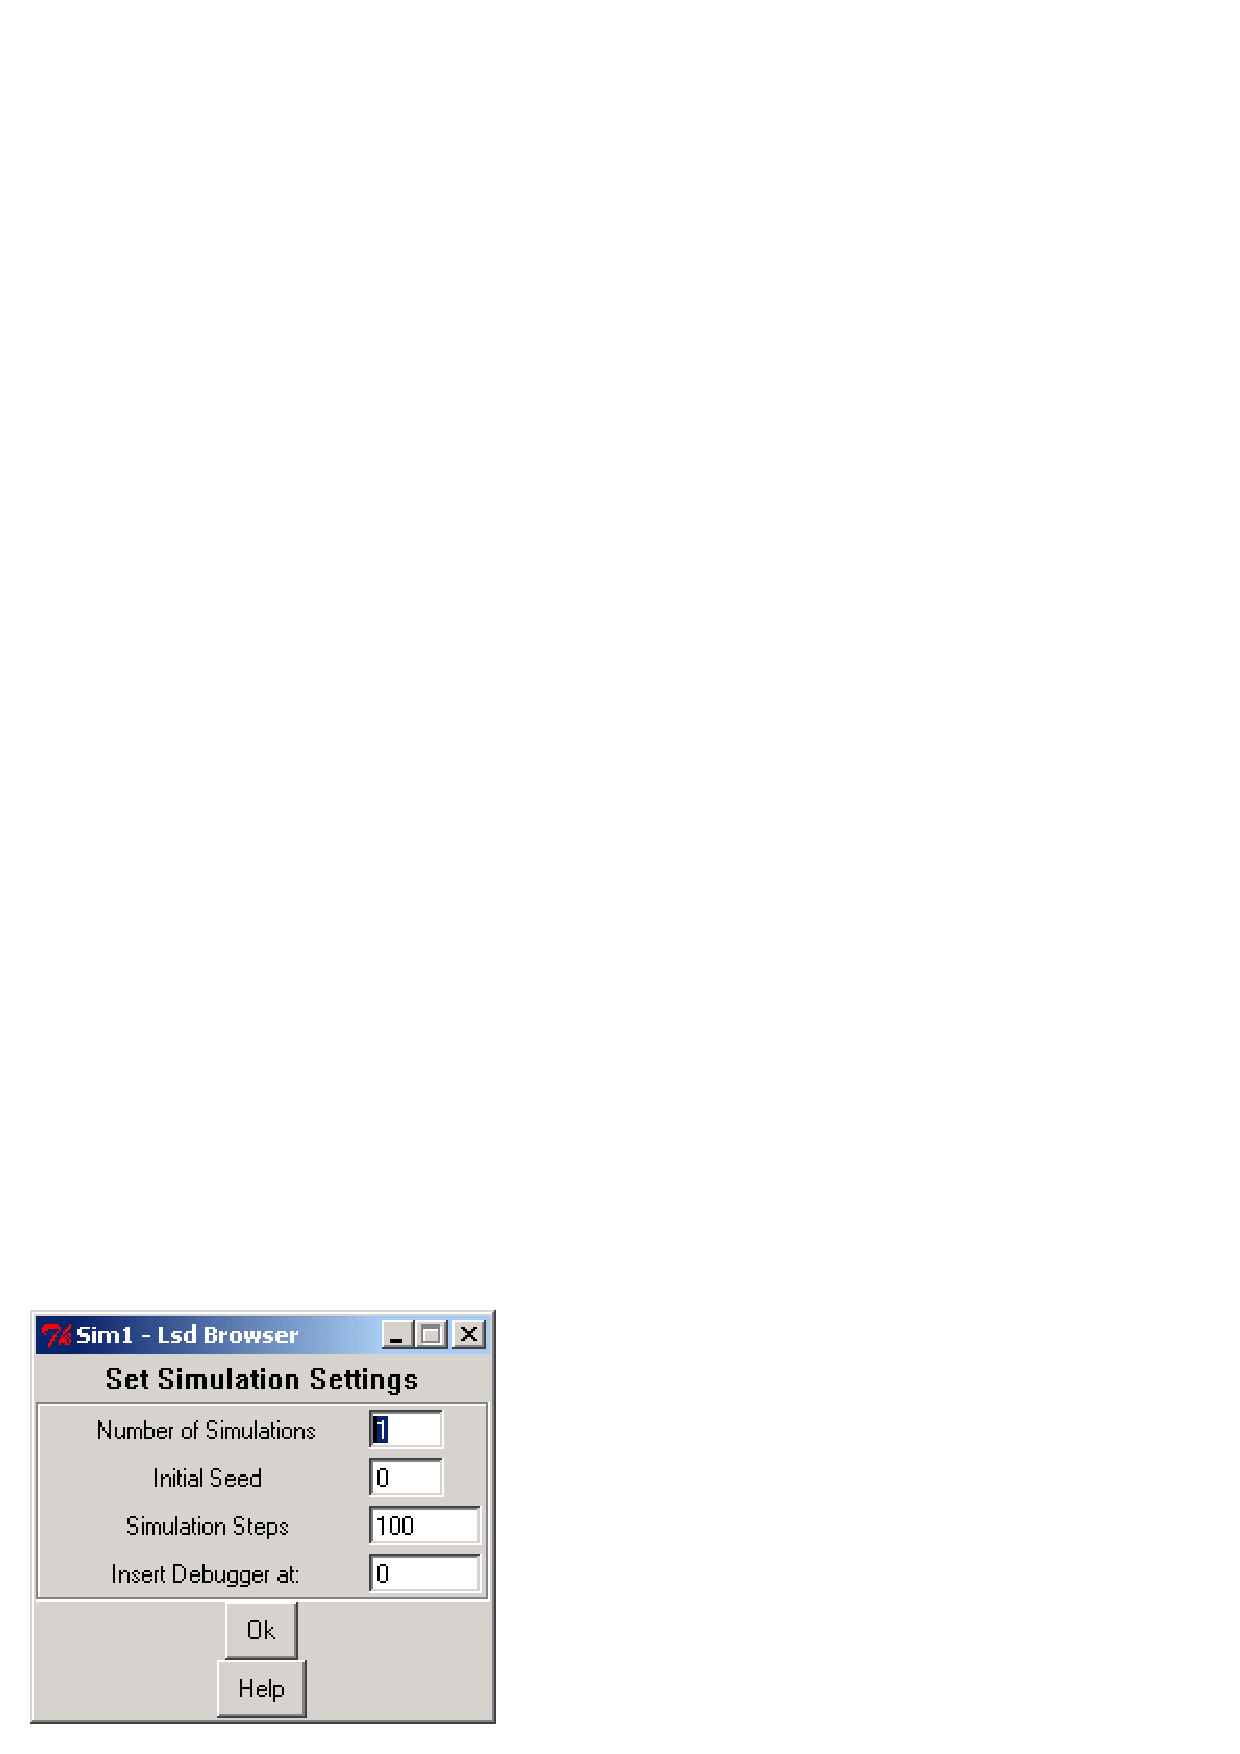
\includegraphics[width=4cm]{simset.pdf}}
  \caption{Simulation options, setting the environment conditions for the model.}
  \label{fig:simset}
\end{figure}

\bigskip

\textbf{Number of simulations}
This value determines how many simulations must be run in sequence. A sequence of simulations consists in many simulations run with the same configuration but using different sets of random numbers. Multiple simulation runs are therefore used to test the robustness of results against variations due to random events.


If this option indicates a single simulation run (value 1), then the system will execute the simulation and, at the end, will retain the simulation results in memory, to be analysed by the Analysis of Results module. If more than one simulation is requested the system produces the first simulation, saves the results in a \LsD result file, re-load the configuration and execute again a simulation run after increasing the seed for the pseudo-random number generator, in effect using a different set of random values.

The result files saved during multiple simulation runs are labeled after the configuration file, extended with the number of the pseudo-random seed generator. Therefore, any simulation  saved during a multiple run can be reproduced using the configuration and the seed indicated. For example, if the configuration contained in the file \code{MyConfig.lsd} is defined to run 10 simulations with initial seed 2, the simulation results will be stored in files named from \code{MyConfig\_2.res} to \code{MyConfig\_11.res}. The result files can be loaded collectively in the Analysis of Results module analysing single simulation runs or comparing the patterns across different runs.

Collective simulation runs generate also a file (named after the configuration and extension \code{.tot}) containing the very final value for each element in each line, and as many lines as the number of simulation runs. This file can be loaded also in the Analysis of Result module, although for this case the ``time steps'' will actually refer to different runs.

It is worth notice that multiple simulation runs are rarely necessary in \LsD. Robustness against random variations may be produced simply multiplying the number of objects in the model. Multiple runs are necessary only when the model dimensions are so large that they wouldn't fit in the computer memory, but are small enough that it is not worth to run in batch mode.

\bigskip

\textbf{Initial seed} 
The random numbers used in stochastic simulations are in effect pseudo-random values generated by means of deterministic functions. This functions produce sequences of values that have the statistical properties of the random function requested. The \textit{seed} for pseudo-random functions initialize the function so that it will generate a given series of (pseudo-)random values. Using twice the same seed will therefore generate the same series of values. When a simulation starts the \LsD model program initializes the pseudo-random functions with the seed specified in this box. Therefore, the same model using the same random values will replicate exactly the same result. Using different seed will instead use different pseudo-random values.

\bigskip

\textbf{Simulation steps} 
Number of time steps to be executed in the simulation run. Note that the modeler may use a command in the equations to close the simulation run in advance, typically under certain conditions. Moreover, users can choose to stop a simulation run at any moment.

\bigskip


\textbf{Insert debugger at} 
Indicate the simulation time step at which to enter in debug mode. At the indicated time step the model will start controlling whether the variables or functions computed have been marked as to be debugged. If one of these is encountered, the system interrupts the simulation just at the end of the equation computing the new value for the element. When the simulation is interrupted in debug mode (which may happen also when an error occurs, such as a division by zero) the system shows the Lsd Debugger interface, showing every detail of the model (see paragraph \ref{ssec:debugger}, p. \pageref{ssec:debugger}).

Inserting in this box values lesser than 1 or above the maximum number of time steps have no effect.


\bigskip

\textbf{Print until stack} 
In some cases, generally for optimizing purposes, it may be relevant to know the exact order of completion of equations within a time step. This order is determined by the \LsD simulation manager at run time, depending on the state of the model at each time step. The \LsD simulation manager tries to compute the equations for all the variables in any object of the model, starting from \lsd{Root}, and then going ``down'' in each object. Normally, equations for variables contained in ``higher'' objects are executed before those for variables of lower objects. However, in some cases this is impossible, since the equations for high objects' variables necessitate the updated value of variables contained in lower objects. 

An equation (say \lsd{X}) being executed because of normal updating required by the \LsD simulation manager is said to be executed at ``stack 0''. If such an equation requires the value of another variable (say \lsd{Y}) not yet updated, the equation for \lsd{X} cannot be completed. It is therefore interrupted (placed on the \textit{stack}), and the equation for \lsd{Y} starts to be executed. This latter equation is said to be executed at stack 1. In turns equations computed at stack 1 may require the values of other values, which will be produced by equations computed at the next stack.

Reading the print-out of the stacks involved in a simulation step, and the label of the variables computed, allow to interpret the order of completion the \LsD simulation manager managed to find (among the generally many feasible). 

This option allows to specify the ``depth'' of the stack one is interested to read. Setting this value at, say, $k$ will generate in the log window a line for each element computed at level $k$ or below. Each line will indicate various information, including the equation result value, the ``triggering'' variable (which variable at stack level $k-1$ requested the value) and the identification tag of the objects containing the variables. Moreover, the lines will also provide the time necessary for the equation to be completed.


\subsection{\menu{Remove debug flags} }
Variables and functions marked to be debugged cause the simulation to stop when the debug mode is inserted. This command removes all the debug marks, or flags, from every element of the model.

\subsection{\menu{Remove save flags} }

The values generated for any element during a simulation run are normally deleted as soon as they are no more necessary to compute the subsequent steps. The modellers need to explicitly indicate which elements' values need to be saved for post-simulation analysis. This command removes all the flags for every element of the model possible marked to be saved. If a simulation is run just after this command, no data will be available for analysis.

\subsection{\menu{Remove plot flags} }

During a simulation run it is possible to generate a dynamic graph for the values of some elements. Using this command all elements possible marked to be plotted dynamically during a simulation run are removed, and no dynamic graph, or run time plot, will be produced.

\subsection{\menu{Show elements saved} }

This command generates a list in the log window for all the elements marked to be saved in the model. It has no effect on the configuration of the model.

\subsection{\menu{Show elements to observe} }

Modellers can mark some elements of the model as series relevant to be analysed. This option is independent from the indications of which elements are actually saved during a simulation run, so that a modeller may indicate with the \menu{observe} flags the meaningful elements for the model, while setting a different set of values to be saved.

This command generates a list in the log window for all the elements marked as worth to be observed in the model. It has no effect on the configuration of the model, but the list of elements worth to be observed is given a prominent role in the automatic documentation of the model.

\subsection{\menu{Show elements to initialize} }

By defaul \LsD forces the modeller to assign initial values to all the parameter of the model and all the lagged variables. However, frequently the initial values for many of such elements have no effect on the model results, because, for example, the model generate its own ``customized'' initialization. The user can indicate the list of the elements whose initialization is mostly relevant for the model results, as marking them ``to be initialized''.

This command generates a list in the log window for all the elements marked whose initialization is considered as particularly relevant. It has no effect on the configuration of the model, though the elements marked as relevant  to initialize are given a prominent role in the automatic documentation of the model.

\subsection{\menu{Remove run time plots} }

The windows containing the dynamic graphs during simulation runs are ``sticky'' and cannot be removed by the usual commands for closing windows. This command removes permanently all the run time plot windows from the screen.


\section{Menu \menu{Help}}

Users may need assistance on the use of the model in two respects. Firstly, they may need help on the use of the \LsD interfaces, commands, meaning of error messages, and any other possible aspect of the \LsD system in general. Secondly, they may need to understand aspects of the model not easily accessible by the \LsD browser. For the first type of issues the entry \menu{\LsD help} gives access to the \LsD manual included in the \LsD distribution. Concerning the information on the model use the second entry \menu{Model Report}, which opens the model report for the configuration used.

\begin{figure}[ht]
  \centering
 \fbox{\includegraphics[width=12cm]{ex_report.pdf}}
  \caption{\LsD model reports are HTML files automatically created describing the elements contained in the model and presenting them in a variety of formats, from textual only to the actual code and values used.}
  \label{fig:ex_report}
\end{figure}

\LsD model reports are HTML files containing all the information contained in the model, presented in different formats, and enriched by hyperlinks allowing to follow the model description according to the preference of the reader.


In a model report there is an introductory section, and three sections for as many lists of the model elements, with  links among related elements within the same sections (e.g. parameters used in an equation) or to other sections (for the same element).

The introductory section includes a textual description of the model and list the main elements to initialize and those containing the main results. As for the other lists the entities are grouped in tables listing sequentially the elements of a single object. Links allow to jump to related objects and/or elements.

The second list provides for each variable and function the actual code used for to compute the element, including also the list of the elements whose values are used in the code. For any element, this list provides the list of equations making use of their values.

The third list includes all the initial values for the elements whose initialization may affect the model.

The structure of the model report is such that users with different programming experience can be provided with the best suited form of documentation. Moreover, the hypertextual format allows users to skip through technical variables, such as averages etc., and focusing only on the interesting parts of the model. Lastly, model reports are easy to transfer and use (basically, they are text files, opened with any web browser), and easy to generate.

If the model report does not exist, the user can open another HTML file, possibly referring to the report of another configuration of the same model. In generaly, however, it is necessary to create a model report from the scratch. This can be done using menu \menu{Model}, which allows to create the model documentation automatically (endowing the model elements with all the information automatically accessible) and the create the model report.


\section{Module \menu{Set Objects' number}}\label{ssec:numobj}

This module determines the number of copies for the objects in the model.

\begin{figure}[ht]
  \centering
 \fbox{\includegraphics[width=10cm]{objnum.pdf}}
  \caption{\small The main window to set the number of objects presents each type of object with their number of copies in the present model configuration. Clicking on this number it is possible to modify the number of copies. Note that the window may be set to hide the number of lower hierarchical levels, in order to identify more quickly the groups of higher level objects.}
  \label{fig:objnum}
\end{figure}

The module report the number of copies  in different lines. The labels of the objects are indented on the right following their parent objects, that it, the objects they descend from. Given the number of objects up in the hierarchy, there will also be consequently groups of descending objects. Hence, each line refers to the ordinal number of  the copy each group of object descends from. 


Clicking on a group of objects, contained in specific copies of higher order objects, it is possible to set the number of objects for that ``branch'' of the model tree independently from the other groups of the same object in other parts of the model.


Besides the setting for individual groups of objects, the module offers also the possibility to modify at once every group of that object in different ``branches'' of the model structure. Suppose your model includes 3 copies for \lsd{Market}, each containing 1 copy of \lsd{Supply}. In the 3 resulting groups of objects there can be a different number of copies of \lsd{Firm}. Suppose that now you want to increase the number of \lsd{Firm}'s to 200, but not only in a single copy of \lsd{Market}, but in all the copies of \lsd{Market} of the model. As indicated in figure \ref{fig:objnum1} it is possible to mark the option to extend the chosen number of descendants to the whole model, or to the specific branch of the model structure.


\begin{figure}[ht]
  \centering
 \fbox{\includegraphics[width=4cm]{objnum1.pdf}}
  \caption{\small When setting the number of a group of object contained in a complex model structure, it is possible to apply the new number of objects to all groups of the concerned objects at different levels in the model.}
  \label{fig:objnum1}
\end{figure}

The interface determining the scope of the changes allows to choose not only among the objects one layer above, as in the example case, but to any possible higher layer. For example, suppose that \lsd{Market} is defined as contained in objects of type \lsd{Country}. One may decide whether the change should be applied to a single \lsd{Market}; to all \lsd{Market}'s in a single \lsd{Country}; or to all \lsd{Market}'s in all \lsd{Country}'s. 

The system always appends new copies after the set of previously existing copies. The new copies of the objects  will replicate the content (e.g. parameters' values, number of descendants, etc.) of an example object. By default the system uses the very first copy of the object as example, but users can choose a different one. This is done inserting the ordinal number of the desired example copy in the field \menu{Copy from instance: }. For example, if the first \lsd{Market} contains 10 \lsd{Firm}'s and the user wishes to use the first object in the second \lsd{Market}, then the field should indicate 11. For complex models the ordinal number of a specific copy may be difficult to calculate. Clicking on \menu{Compute} helps to find out the ordinal number of a copy by specifying the ordinal numbers by different layers of the model.

In case the new number of copies of an object is smaller than the previous value, the system by default would remove the last copies in the set of objects, but the user can indicate specifically which copies must be removed. For example, suppose you have a model containing three copies of an object. Setting one to the copies of this object it is necessary to remove two previously existing copies. If the system decides automatically the copies to remove, it applies the rule that the last copies in the sequence of previously existing objects should be removed. Therefore, the copies removed will be the second and the third, leaving only the first copy. Alternatively, the user can decide to choose the copies to remove. A sequence of windows will ask the ordinal numbers of the copies to remove. For example, the user can indicate the first and third copy to remove, and the new configuration will retain only the second copy. The option to specify each individual copy to delete cannot be used when the new number of objects is applied to several groups, for example, to all groups of \lsd{Firm}'s in the previous example. In this cases, the system always remove the last copies in each group.

\section{Module \menu{Initial values}}\label{ssec:initval}

This module allows insert the initial values for all the copies of a specific object. The initial values for a simulations are all the parameters, lagged variables and lagged functions present in the model, that is the values necessary to compute the equations at the initial time step(s).

Parameters obviously need to be assigned an initial value\footnote{Note that modelers may have equations to overwrite the value for parameters, though this may produce uncertain results given that the system is not able to control the timing of parameters' value changes.}. Lagged variables are variables whose values are used in some equations of the model with a lag, that is, it is the values from previous time steps. In the earliest time step of the simulation, $t=1$, there are no past values to be used, and therefore the user must explicit provides this value, to be associated to the elements' values at time $t=0$, $t=-1$, etc.

Lagged functions are functions whose values are required for previous computation of the function. In this case, the very first time function's values are used there are no previous values to be supplied to the ``calling'' equation, and, again, the past values must be initialized.

\begin{figure}[ht]
  \centering
 \fbox{\includegraphics[width=10cm]{init1.pdf}}
  \caption{\small Module to set initial values for the elements requiring initializations within one type of object. Elements are presented in rows and each column refers to a copy of the object in the model.}
  \label{fig:init1}
\end{figure}

The module to insert initial values concerns all elements to be initialized contained in one single type of object. The module's interface provides one row for each element to initialize (and each lag for past variables' and functions'). The columns refer to the different copies of the object. They are identified with a ``tag'', a combination of digits referring to the ordinal copy of the objects containing the elements and all objects in higher layers. For example, a model containing objects \lsd{Market} in turn containing objects \lsd{Firm}, the columns for the initial values of elements in \lsd{Firm}'s will contain two digits: the first for the ordinal copy of \lsd{Market} and the second for the ordinal copy of \lsd{Firm} in that copy of market. A tag may for example be $12 - 25$, indicating the initial value for the element indicated in the row and the copy contained in the $25^{th}$ copy of \lsd{Firm} among the set of this object contained in the $12^{th}$ \lsd{Market}. A similar model composed by objects \lsd{Country} containing \lsd{Markets}, then the initial values for \lsd{Firm} will be composed by three digits, as in $2 - 12 - 25$: $2^{nd}$ \lsd{Country}, $12^{th}$ \lsd{Market}, $25^{th}$ \lsd{Firm}. The tag for the cell with the cursor is reported in the bottom line of the initial values interface

The interface for the initial values allows to insert manually the initial values for an element. Typing one value and pressing the key \menu{Enter} moves to the next cell. This interface can contain a maximum of 100 columns, assuming that larger number of initial values will never be assigned manually, but using an initialization function.

\subsection{Initialization functions}\label{sssec:setall}

The initialization functions are mathematical expressions assigning the values to the sequence of initial values for an element, that is, all the initial values for, say, a parameter in every copy of the object containing it. For example, an initialization function may consists in assigning identical initial values to all the copies of the element. Initialization functions obviously affect all copies of the element to initialze, even beyond the 100 shown in the module's interface.

\begin{figure}[ht]
  \centering
 \fbox{\includegraphics[width=6cm]{setall.pdf}}
  \caption{\small The \menu{Set all} buttons permit to apply an initialization function to all the copies of one element.}
  \label{fig:setall}
\end{figure}


The initialization function for an element to initialized are determined using the button \menu{Set all} appearing in the beginning of each row, just after the label of the element. This interface is very flexible, providing an extended set of different initialization function, besides the possibility to control which copy of the elements need to be assigned with that function. For example, one may use a given initialization to the first half of the elements and another for the second half. 

The \menu{Set all} interface is composed by three sections: the nature of the initialization function; the values of parameters for the initialization function; the choice of pseudo-random values; frequency of application; the extension of its application.

The initialization functions available are the following, each of which uses the two cells containing numerical values in different ways. In the following we will refer to these numerical values as those indicated in the first and second cell.

\menu{Equal to}. Assign the same value, as indicated in the first cell, to all the copies of the element.

\menu{Range}. Assign equally spaced values starting from the value in the first cell and finishing to the value of the second cell. For example, suppose that there are 100 copies of the element to initialize, and the initialization function \menu{Range} is used with values from 0 to 100. Then, the first and last copy of the element will be 0 and 100, respectively. The intermediate cells will have equally spaced values: 0, 1.010101, 2.020202, 3.030303, etc.

\menu{Increasing}. Assign increasing values to the copies of the element to initialize starting from the value indicated in the first cell and increasing of the value in the second cell for each subsequent copy. For example, using \menu{Increasing} and setting the values of the data cells to 10 and 1 respectively, the initial values will be: 10, 11, 12, etc.

\menu{Increasing (group)}. This initialization function is identical to the \menu{Increasing} one, but it is re-set to the starting value for each separated group of objects. For example, consider a model composed by objects \lsd{Firm} contained in \lsd{Market}. Suppose there are many copies of \lsd{Market}, each containing many copies of \lsd{Firm}. Initializing an element contained in \lsd{Firm}, using this initialization function will assign increasing values to the set of elements contained in the first \lsd{Market}. Then, the initial value for the copy of the element in the first \lsd{Firm} contained in the second \lsd{Market} is reset to the starting value, equal to the value used for the first \lsd{Firm} in the first \lsd{Market}. 

\menu{Random (uniform)}. Assign a real number as a random value for each element to initialize, using a uniform random function whose lower and upper limits are determined by the values in the first and second cells respectively.

\menu{Random integer (uniform)}. Generate an integer number as a random value for each element to initialize, using a uniform random function whose lower and upper limits (included) are determined by the values in the first and second cells respectively.

\menu{Random (normal)}. Generate a real number as a random value for each element to initialize, using a normal random function whose mean and deviation are those indicated in the first and second cell respectively.

\menu{File}. Load the initialization values from a file. Files for initial values must be text files containing one single column. The first element of the column is ignored, assuming to be a label.

\menu{Sensitivity}. The user is requested to indicate in the first cell the number of values to use for the element. On confirmation a new window will ask for the list of the values, separated by newline or spaces (may even be pasted from the clipboard). If the list contains fewer value than those specified in the first cell the remaining ones will be considered to be 0. This initialization does not modify the initial values of the model, but allows to generate automatically configurations for sensitivity analysis. When two or more elements are initialized, the  \menu{Data / Sensitivity} (see paragraphs \ref{sssec:senspar}, p. \pageref{sssec:senspar}) creates configurations including all possible combinations for the values of the elements initialized as to be included in the sensitivity analysis.

\bigskip


The random initialization functions can be assigned using a specific seed generator. Using a specific initialization ensures that the random values they are drawn from the same or a different (pseudo-)random sequence as other initializations. Checking on the option to use the seed, the random sequence will be regenerated using that seed.

\bigskip

The two sections in the bottom of the initialization window allow to specify which sub-set of the copies of the element must be initialized according to the specified function. The first of these section concerns the \menu{Frequency} of the initialization, while the second concerns the \menu{Extension}. 

By default, the system applies the function to every copy of the element, that is, it has a frequency of 1. Setting a higher frequency $N$ (say, for example, 3), the initialization function will regularly skip $N-1$ copies and apply the initialization rule to the $N^{th}$ copy, in the example the third. If the option \menu{Fill in} is not checked, the copies in between those initialized are not set, leaving the previously existing values. If, instead, this option is marked, the intermediate copies will be set with the values previously generated by the initialization function. For example, suppose to have selected the function \menu{Increasing}, starting from 10 and with step 1. If the frequency is 3 and the option \menu{Fill in} is on, then the sequence of initial values for the copies of the elements will be: 10, 10, 10, 11, 11, 11, 12, 12, 12, etc.

Concerning the extension, the user can choose to apply the function to all the copies of the element in the model, or only to a range of contiguous elements (that is, of elements contained in contiguous objects). The two cells in this section refer to the first and last object containing the element of the model, which must be indicated with the sequential number of the objects. To identify the sequential number it is possible to right-click the cells opening the interface to individuate the sequential number of an object by giving the ordinal number of the higher level objects (see figure \ref{fig:objnum1} at page \pageref{fig:objnum1} and the related text).

The final option \menu{Update description} does not affect the values inserted in the model but only the documentation. If checked on, the system will automatically update the description of the initialization concerning the element, specifying the function used and its values. If the function used concern all the elements, then the new description will replace the previous one. Otherwise, it will be appended, possibly requiring the editing of the modeller in case of potential confusing text.



\section{Module \menu{Analysis of Results}}\label{ssec:analres}

\begin{figure}[ht]
  \centering
 \fbox{\includegraphics[width=12cm]{AnaResult.pdf}}
  \caption{\small Main Analysis of Result window. Series available are listed in the left-hand box, series to be processed in the central box, and graph produced in the right-and box. The user needs to move some of the series in the central box, select the options and the operation required. The analysis of results module is highly efficient in managing large data sets.}
  \label{fig:anaresult}
\end{figure}



The analysis of results module is designed to present the data produced in (one or more) simulation run(s) in formats suitable for the purposes of the researcher. Here is summary of the functions of the module:

\begin{itemize}
	\item Time series plots. Variables are plotted across time steps.
	
	\item Cross-section plots. Values of different variables are plotted at the same time step.
	
	\item Scatter plots. Variables' values are represented as function of other variables' values, generating both bi- and tri-dimensional graphical representations.

	\item Phase diagrams. Values of a variable at time $t+1$ are represented as function of the same variable's value at time $t$.
	
	\item Frequency histograms. Values across time for a variable, or across variables at a given time, are counted and grouped in frequency classes.
	
	\item Lattices. Values stored in matrices are plotted as lattices.
	
	\item Temporal or cross-section statistics. Descriptive statistics as average and variances can be produced across times or across variables.
	
	\item Options. It is possible to let the system automatically assess the scale of the graphs, or force the extremes of the axis. Other options include the symbols for series (lines or points), grids, colors, labels, etc.
	
	\item Exporting graphs. Plots can be exported as encapsulated postscript files.
	
	\item Exporting data. Series can be exported as text files in a variety of formats (e.g. choosing a separator, or fixed-column lenght; with or without labels, etc.).
	
	\item Gnuplot. The MS Windows distribution includes gnuplot, a specialized graphical package, to produce advanced graphs, for example on data exported from \LsD simulations.
\end{itemize}



The typical use of the Analysis of Results module consists in selecting one or, more in general, a set of series to process; set the options for the type of operation desired; generate the results (graph or statistics); replace the series and continue the process. Eventually, some graphs or data may be exported, or the user returns to the \LsD browser to generate a new configuration and running new simulations.


In the following we report the instructions to perform the operations allowed by the module.

\subsection{Selecting series to process}

The first operation in using the Analysis of Result module (AoR) consists in individuating the meaning of the available series and moving the selected ones in the central listbox.

A simulation model may generate large data sets, composed by several thousands of series each containing thousands of data. For this purpose, the module includes also a powerful selection interfaces, allowing to identify a specific set of series by their labels, values, or positions in the model structure. For this purpose, the system identifies each series by a unique combination of labels and digits, which can be exploited by the user to select series to process with many different criteria. The label of a series contains the following elements:

\begin{verbatim}
Label TAG (TimeStart - TimeEnd) # order
\end{verbatim}

The first components in a series identification is, obviously, its label.  Secondly, each series is associated to a ``tag'', a group of digits identifying the ``branch'' of the model structure in which its object containing the element generating the series was contained. For example, a tag as $X\_Y\_Z$ indicates that the variable was contained in an object placed at the third layer in the model hierarchy (\lsd{Root} is the only object at level 0, level 1 refers to objects contained in \lsd{Root}, level 2 their descendants, etc.). That particular series was contained in the $Z^{th}$ copy of object at level 3, which descended from the $Y^{th}$ copy of the object at level 2, which, finally, was contained in the $X^{th}$ copy of the object at level 1. Note that if a level contains one single instance of an object, then its digit may be skipped, since it is not necessary to identify different series in descending objects.

Finally, the identification includes the time steps at which the copy of the element (that is, the copy of the object containing the element) started to exist in the model and the date at which it was removed. 


The last code is unique ordering value, used for technical purposes and of no interest to users.




The first step in using the Analysis of Result module consists in selecting a group of series from the left box \menu{Series Available} and placing them in the central box \menu{Series Selected}. In order to access the series one can scroll the \menu{Series Available} box, and sort its content in three different modes. Firstly, the unsorted mode (used by default, and activated by pressing button \menu{Un-sort}), list the series according to their position in the model: first the series generated by elements in high level objects, and followed by their descendants, then series from elements from the subsequent objects. This sorting mode is useful since arranges the series in a sequence resembling the model hierarchy.

Secondly, it is possible to sort the series in the ascending alphabetical order of their labels. This model is useful to identify a series without knowing their location in the model structure. Press button \menu{Sort} to generate this sorting.

Thirdly, it is possible to sort series in alphabetical order but putting firstly all the series contained objects still present in the model (not removed) at the final time of the simulation, and then the series according to the descending time step of their removal. This sorting mode (activated by pressing \menu{Sort (end)}) is useful when the model stores many variables from objects created and destroyed during a simulation run.

After having sorted the sets of series available as suited, the selection of the series one wants to process can take place by the usual selection standards: click and drag, use of the \menu{Ctrl} key to add a new item to the selection; use of the key \menu{Shift} to add sets of items to the selection and removing previous ones, etc. Double-clicking on a series moves this directly to the central box, while it is necessary to click on the button \menu{$>$} to move there the whole selection from the left box.


\subsection{Advanced selection}
The system to select and move the series is practical only insofar users need to select a few series. However, \LsD simulations can produce hundreds or thousands of series, and the user may need to select all of them, or a well specified sub-set. In these cases, using the mouse to select the series is impractical, or totally unfeasible. An alternative selection mechanism consists in pressing the right-button of the mouse on one of the series that the user needs to select.


\begin{figure}[ht]
  \centering
 \fbox{\includegraphics[width=5cm]{sselection.pdf}}
  \caption{\small Clicking with the right button on a series a powerful selection mechanism allows to choose among the series available with the same label.}
  \label{fig:sselection}
\end{figure}

This selection mechanism allows to choose the series according to three possible criteria of filtering the series with the specified label.

Firstly, and most frequently used, the option \menu{Select all the series} allows to select all the series with the specified label in the model. As mentioned, the label concerns the series the mouse has been right-clicked, so that, in effect, the user needs not to type any text at all. This is the default option.

Secondly, it is possible to filter the series with the specified label according to the tags, that is, to the obejcts containing the series. This option is used by marking the window section \menu{Select for series' tags}. This section contains a number of entry cells equal to the hierarchical level of the object containing the element specified (in the example, three cells since the series specified concern an element located in the third level). As mentioned above, this number is equal to the number of digits forming a series' tag. The user can enter integer values in one or more of the cells, or leave them empty. The values entered in these entries will be used as reference values for the condition chosen in the last section of the window \menu{Set condition to meet}. For example, using the default condition \menu{Equal to: =}, the system will select all the series having the elements of the tag equal to the value(s) entered in the entry cells (empty cells are read as accepted condition). Using, instead, condition \menu{Larger: $>$} the system would select all the series with tag's values higher than those specified in the entry cells.

The third filtering mechanisms (\menu{Select for values of another series}) is based on the conditional filtering based on the values of some element of the model, whose series is among those available. The user must enter: the label of the element by which the to filter the series; the time step of the series to consider; and a reference value. The elements used for the conditional part must be located in the same objects as the elements whose series are selected. The system will compute for each copy of the objects the value for the conditional element (at the specified time step). It will then evaluate whether this element's value satisfies or not the condition indicated in the last section, as compared to the reference value. Only the series whose associated element satisfy the condition will be selected. 

For example, consider to use this filtering system and specifying: label for the filtering element \lsd{Age}, time step 100, comparison value 10, and condition \menu{Smaller: $<$}.  The system will select only the series with the specified label being contained in the objects that contained the element \lsd{Age} at time 100 with values smaller than 10.


\subsection{Graphs general options}

The procedures to create any type of graph follows the same steps: insert one or more series in the \menu{Series selected} box; set the options for the graph; set the options for the type of graph; press button \menu{Plot}. For all graphs the user can set the following options.

\menu{Use all cases} - \menu{From case ... to case ...}. If the first option is used the system will use all the data available for the elements plotted. If different series have different starting and final times the time series graphs will ignore data for missing times. For cross-section graphs series missing the relevant data will be ignored. Using the second option (relevant only for time series graphs), the user must specify the time step to be used as origin of the graph and that for the last time step. Notice that when using the automatic option to use all cases, the system inserts in the cells the first and last case (i.e. time step) used.

\menu{Y self-scaling} - \menu{Min. Y ... Max. Y}. The first option lets the system compute automatically the vertical minimum and maximum values. Note that the maximum value is not the actual maximum value of the highest series, but extends a bit the range of the vertical axis to allow for the points plotted to appear in the window. The second option allows the user to force specified values for the minimum and maximum vertical axis.

\menu{Y2 axis}. This option is used only for time series sequential plots, and requires the use of the option \menu{Y self-scaling}. When this option is checked on the system will use two independent vertical axes. The user needs to specify the series from which the second vertical axis is used. All the series before the indicated one will make use of the first vertical axis. This plot allows to plot different series normalized on two independent scales.

\menu{Title}. This entry is automatically filled with the identification label of the first series entered in the \menu{Series selected} box. The text in this series is used to name the graph generated, and is used only to identify the different graphs. Note that each graph is assigned also a progressive index.

\menu{No color}. Generates black-only or gray scale graphs, depending on the type of graph.

\menu{Grids}. Plots a grid in the graph, for readability purposes.

\menu{Lines} - \menu{Points}. Use lines (connecting separated points) or points only. The entry cell along the points' option allows to set the points' size.

Menu item \menu{Color}. This menu allows to modify the color associated to the indexes. This color will be used to differentiate the series according to their order.
 
\subsection{Graph windows' features}

The graphs generated are normally\footnote{Some 3D graphs can be created in separate windows managed by GNUPLOT.} stored in \LsD independent windows. These windows have many features useful to interpret the results contained in the graph.

The lower border of the window shows the coordinates of the plane corresponding to the mouse pointer position. Moving the pointer over one series shows the name of the series on the lowest left corner of the window. Cross-section graphs reports also the order position of the series concerned.

Double-clicking anywhere on the graphs brings the main AoR windows on the foreground. 

Pressing the \menu{Shift} key and clicking allows to add a text label on the graph, which can be then moved around with the mouse.


In the following we report some examples of graph generated with the AoR window depending on the options chosen.


\subsection{Graph type \menu{Time Series - Sequence}}

This graph generates one line for each series, placing the time on the horizontal axis. 

\begin{figure}[ht]
  \centering
 \fbox{\includegraphics[width=7cm]{example_graph.pdf}}
  \caption{\small The default options produce a standard graph with time on the horizontal axis and each series selected generates one line. Moving the mouse on the area of the graph reports the pointer's coordinates, and, crossing a line, its label.}
  \label{example_graph}
\end{figure}

\clearpage

\subsection{Graph type \menu{Cross section - Sequence}}
This options generate a graph containing one or more line referring each to a specified time step and reporting all the values for the different series for that time step. This graph requires additional information: the time step(s) to use and the ordering of the variables. When pressing the button \menu{Plot} with these options a new window asks for the necessary information (figure \ref{fig:crosssection}).

\begin{figure}[ht]
  \centering
 \fbox{\includegraphics[width=7cm]{crossection.pdf}}
  \caption{\small Cases to be used as ``variables'' for cross-section plots are inserted in this window, by typing the times to appear as lines. By default, or pressing the \menu{No Sort} button, the order of the series on the horizontal axis is the same order of the series in the series available box. Alternatively, it is possible to sort the series in ascending or descending order pressing the relative buttons when a time step is highlighted.}
  \label{fig:crossection}
\end{figure}


The user must type at least one time step (in the top-left entry cell), and pressing the button \menu{Add} for each of them (or just the \menu{Enter} key). The inserted cases will appear in the box below the entry cell. Cases can be removed by selecting them and pressing \menu{Delete}. When all the cases have been inserted the user can highlight one of them and press the one of the buttons to sort the series. The order of the series as appearing on the horizontal graph will be then re-arranged to sort the series depending on their values in respect of the chosen time step.

The window has also a hidden feature. Pressing the following combination of keys, and using the the content of the entry cell, the system automatically add whole batches of series. The combinations are the following:

\begin{itemize}
\item \menu{Controf+f} (\textit{from}): use the value as starting time.
\item \menu{Controf+t} (\textit{to}): use the value as final time. 
\item \menu{Control+z}: add to the list of time steps selected all the times from that indicated as starting time to the final time.
\item \menu{Control+x}: indicate a step, so that if 100 is the starting time and 10 is the step, the times inserted will be: 100, 110, 120, etc.

\end{itemize}
 
Pressing \menu{Continue} will generate the graph, while button \menu{Abort} terminates the window without generating the graph. The graph will show on the horizontal axis the series and will link the points corresponding to the same time step for each series.


\begin{figure}[ht]
  \centering
 \fbox{\includegraphics[width=7cm]{cross_section.pdf}}
  \caption{\small Example of a cross section sequential graph. 100 series selected have been evaluated at time 300, and ordered according to their descending values at the chosen time step. The mouse pointer crossing the line indicates the series concerned and its ranking order.}
  \label{fig:cross_section}
\end{figure}

\subsection{Graph type \menu{Time Series - XY plot}}

These options produce a scatter plot where the values of some series are used as independent variables and others as dependent, creating graphs where each point is a single time step. Choosing the option \menu{Lines} the system tries to interpolate the points forming smoth curves. It is anyway better to use the option \menu{Points} for most of cases.

The system behaves differently depending on the number of series in the \menu{Series Selected} listbox.

\subsubsection{Single series}

When the system finds a single series it generates a phase diagram where each point is defined at the coordinate  $X_t$ on the horizontal axis and $X_{t+k}$ on the vertical axis. In this case the system asks for number datum from the series and the number of lags $k$. The system also offers the possibility to generate the graph as image in a standard \LsD graph window or in a higher quality gnuplot window (default option). As all gnuplot windows there are special functions embedded in the window, such as the possibility of rotating the graph and direct exporting to file; these options and their control depend on the operative system.

Optionally, the user can plot a line in the graph placed at 45'. 

\subsubsection{Two series}

When two series are present in the \menu{Series Selected} the system directly generates the scatter plot where the values of the first series are reported on the horizontal axis and the values of the second are measured on the vertical axis.

\subsubsection{Three or more series}


When plotting this graph with more than two series selected, the module generates a new window, asking for additional information concerning the graph.

\begin{figure}[ht]
  \centering
 \fbox{\includegraphics[width=4cm]{23d_time.pdf}}
  \caption{\small To create a scatter plot from time series the system asks whether the graph should be 2D (one independent variable) or 3D (two independent variables). For 3D graphs it is possible to use gridded data (interpolating points) and generating color mapped surfaces. Finally, the user can decide to have the graph as a standard \LsD graph window (low quality), or having the graph plotted in an interactive gnuplot window.}
  \label{fig:23d_time}
\end{figure}

The user can choose a bi-dimensional scatter plot (2D) or a tri-dimensional (3D) one. In the first case the first series in the set of series selected will be used as independent variable (measured on the horizontal axis), while the second and following series will be plotted generating as many independent lines, one point for each time step. 

Choosing 3D graphs there are several options. The default option generates a 3-dimensional space where the first and second series are used as coordinates on the plane. Any subsequent series is considered as independent surface measured on the vertical axis. Figure \ref{fig:example_scatter_time} shows an example of a 3D scatter plot with two independent series defined on the same plane.

\begin{figure}[ht]
  \centering
 \fbox{\includegraphics[width=7cm]{example_scatter_time.pdf}}
  \caption{\small Example of a 3D scatter plot computed across time. The model generating the data is $Y_t=K_t^\alpha*L_t^{1-\alpha}$. 10000 random values for $K$ and $L$ are used to compute two different series of $Y$'s using different $\alpha$'s. The plot is generated with lines and gridded data.}
  \label{fig:example_scatter_time}
\end{figure}

The second option generates, in effect, bi-dimensional graphs placed, however, in a three dimensional graph where the time dimension is one of the two dimensions on the horizontal plane.

The third option plots each series independently as time series, using the ranked position of the series as one dimension of the plane, and the time as the second dimension.

The last technical option allows to choose between a standard \LsD graphical window or a high quality gnuplot one. As all gnuplot windows there are special functions embedded in the window, such as the possibility of rotating the graph and direct exporting to file; these options and their control depend on the operative system.


\subsection{Graph type \menu{Cross section - XY plot}}

These options generate a graph at a single time step, indicated in the first cell of the option window, using the data from all the series selected. The system divides the selected series in blocks, with each block providing the sets of values to be used as variables for the axes of the graph.

\begin{figure}[ht]
  \centering
 \fbox{\includegraphics[width=4cm]{cs_xy.pdf}}
  \caption{\small Plotting a cross section scatter plot use only one time step value from each series selected. The graph generates the horizontal axis (or axes, for 3D graphs) using the values from the first (or first two) blocks of variables, while the subsequent blocks will provide the values for the dependent variables.}
  \label{fig:cs_xy}
\end{figure}

In case of 2D graphs the system by default divides the available series in two halves, assuming a single dependent variable. In this case the first half provides the horizontal coordinates of the points and the second half provides the complementary vertical coordinates. Users can indicate a larger number of dependent variables. Indicating the series must provide data for $k$ dependent variable the system divides the data in $k+1$ blocks, where the first block provides the common coordinates for the horizontal axis and the system plots $k$ independent series on the vertical axis. The users must ensure that the number of series is a whole multiple of $k+1$; the system reports the number of points implied by the number of series selected and the indicated number of dependent variables. Figure \ref{fig:xy_cross} shows an example of a 2D graph.

\begin{figure}[ht]
  \centering
 \fbox{\includegraphics[width=7cm]{xy_cross.pdf}}
  \caption{\small Example of a cross section 2D scatter plot using points, represented in a gnuplot window. The series selected contained 200 series. The first 100 provided the values for the horizontal axis. The label reported on this axis is the label for the first series of this block. The second half of the series provided the value (at time step 300) for the dependent variable, again, the label is reported from the very first series in this block.}
  \label{fig:xy_cross}
\end{figure}

\bigskip
In case of 3D graphs the same system applies. The system divides, by default, the series selected in three blocks, using the first two as coordinates for the plane and the third as height of the plotted surface. Similarly to the 2D case, users can set a different number $k$ of dependent variables. In this case the system divides the series selected in $k+2$ groups generating the horizontal plane coordinates with the first two blocks and $k$ independent surfaces on the vertical axis. 



\subsection{Graph type \menu{Histograms}}

\begin{figure}[ht]
  \centering
 \fbox{\includegraphics[width=7cm]{ex_histo.pdf}}
  \caption{\small Example of an histograms. The data are produced by a generating 1,000,000 random draws from a standardized normally distributed  function. The histograms computes the frequency for 50 classes and interpolates a normal function computed with the same mean and variance of the data.}
  \label{fig:ex_histo}
\end{figure}

Clicking on the button \menu{Histograms} generates a graph containing a representation of the frequency of the values indicated in the series selected. The histograms are built dividing the range of the values used in as number of classes, as indicated by the user, with each class having the same width. For example, if the values used to generate a histograms have a minimum of 10 and a maximum of 30 and the user asked for 10 classes, the first class boundaries will be [10-12], [12,14], ..., [28-30]. The system then counts how many values fall in each class and reports on the graphs columns with height proportional to the frequency in each class.


The graphs for histograms show the information on each class when the mouse pointer is moved onto a class, including the class' boundaries and middle value, actual minimum and maximum value in the class, etc. Moreover, the user can ask for the information to be printed in the log window.

Histograms may be computed from a single series using its values across time, or from many series using one single value for each of them. The option \menu{Time series} or \menu{Cross section} determines which type of histograms are computed. When \menu{Time series} is selected, there must be one single series selected, otherwise the system will issue an error message. A maximum of 100 classes can be specified by the user.



\subsection{Graph type \menu{Lattice}}

\begin{figure}[ht]
  \centering
 \fbox{\includegraphics[width=5cm]{ex_lattice.pdf}}
  \caption{\small Example of a lattice. The series selected are taken from a 400 x 400 matrix, represented in \LsD as 400 objects \lsd{Row} containing each 400 objects \lsd{Col}. The series concern an element located in \lsd{Col}, taking values 0 or 1.} 
  \label{fig:ex_lattice}
\end{figure}

Lattices are graphs formed by grids of with each cell colored according to a value specified by a non negative integer. Lattices require to insert as selected series as many series as the number of cells. The system assumes that the series are contained by lines: first all the values for the first line, then the values for the second line, etc. 

The user must provide the data for the time step to be used from the series selected, and the number of columns for the graph. This number must be an exact divisor of the number of series selected, since the division of this two numbers provides the number of lines. The user must also specify the number of pixels to be used for total width and height of the lattice window, which obviously must be larger than the number of lines and columns. See figure \ref{fig:ex_lattice} for an example.


\subsection{Statistics}

%\begin{figure}[ht]
 % \centering
 %fbox{\includegraphics[width=7cm]{ex_statistics.pdf}}
  %\caption{\small Example of descriptive statistics. The data are computed over 10 series for 500 time step each. The values concern average, minimum, maximum and sigma values.} 
%  \label{fig:ex_statistics}
%\end{figure}

The system can compute descriptive statistics from the series selected. The statistics concern average, minimum, maximum, variance and standard deviations of the values indicated. The computation can be performed across time or across series, as indicated by the options \menu{Time series} or \menu{Cross section} respectively. The results will be shown in the log window.

\subsection{Exporting data}

Clicking on the \menu{Save data} button the system exports the values from the series selected in a text file. The data can be exported as \LsD result file or as plain text files. In the first case the data can be uploaded by any \LsD model program using the appropriate command in the Analysis of Result module (\menu{Add Series}).

Choosing to export data as text file it is possible to choose a variety of options, such as the delimiter symbol and names of the variables.


\subsection{Exporting graphs}
Clicking on the button \menu{Postscript} the user can save a graph window as postscript file, for inclusion in a document. 

\subsection{Adding further series}

The values that the user can process in the AoR module are those produced during the last simulation run by elements marked as being saved for this purpose (see paragraph \ref{subsub:opt_ele}, pag. \pageref{subsub:opt_ele}). However, the module allows also to add more series in the set of the available series. Additional series can be obtained pressing button \menu{Add series} in between the two listboxes. 

\begin{figure}[ht]
  \centering
 \fbox{\includegraphics[width=4cm]{create_series.pdf}}
  \caption{\small A single new series can be created as a statistics computed on the data contained in the series selected. The new series can be computed by computing the statistics for each time step across all the series, or for each series across all its time steps.}
  \label{fig:create_series}
\end{figure}

The new series can be obtained from several sources.

\textbf{Current state of the model}. It is possible to insert the data from an element of the model not saved during a simulation run. In this case, the number of new series will equal to the copies of the objects containing the element. Each of the new series will contain a single value, which will be assigned the conventional time step of $t=0$. This series can be used as independent variable in cross-section scatter plots even in case the user specifies different time steps for the dependent variables.


\textbf{Previously saved result files}. User can add new series stored in files previously generated during past simulations. Users can select single files or whole batches of them, as those, for example, generated during batteries of simulations. In this case, the system will add all the new series as contained in the result files, assigning them the original names extended with the letter \menu{F} (so that \lsd{Label} will appear as \lsd{LabelF}). Moreover, these series will have a further digit attached to the tag, indicating a progressive index for any file. The log window will report the code for each file so as to associate series to specific simulation runs.

\textbf{Moving averages from selected series}. If one or more series are reported in the \menu{Series Selected} listbox it is possible to create as many new series computed as moving average of the selected series smoothed over the indicated number of time steps.

\textbf{New series from elaboration of selected series}. The user can elaborate the values from the selected series generating a single new series. The options available are listed as in figure \ref{fig:create_series}.


The options available are the following. By default the system considers the creation of a new series with the same number of time steps as the selected series, and considering the elaboration across the selected series. Alternatively, the user can choose to elaborate the data across time steps to generate a new series having as many virtual time steps as the number of series.

The second option allows to remove from the elaboration outliers, i.e. data too small or too large, where the user imposes the treshold. 

The type of elaboration includes: average; sum; maximum; minimum; variance; standard deviation (times a constant); counting.

Finally, the user can specify the new variable's label and a tag number.


\section{Module \menu{\LsD Debugger\xspace} and \menu{Data Browser}}\label{ssec:debugger}

The \LsD browser shows the content of the model by means of their structure, but does not allow to inspect the copy of each element. The \LsD debugger and the data browser use similar windows to provide access to each individual element of the model, object by object. The data browser is used when a simulation is not running, activated by menu \menu{Data/Data Browse} of the \LsD browser. The \LsD debugger is instead used during a simulation run, when it is interrupted. The \LsD debugger includes, besides the data browser, also the commands to control the simulation run. In the following we will refer for rbrevity only to the \LsD debugger, though all the commands work also for the data browser.


\begin{figure}[ht]
  \centering
 \fbox{\includegraphics[width=9cm]{debugger.pdf}}
  \caption{\small Debugger set on the equation for \lsd{Purchase} at the 42$^{nd}$ time step. The debugger window, as the data browses, show the state of a model for each individual copy of an object. The user can observe the state of the elements within the objects, moving through the object structure, modify the values, activate equations, analyse the results, and continue the simulation run.}
  \label{fig:debugger2}
\end{figure}

The \LsD debugger shows the state of one copy of an object. Starting from the button, the debugger window includes: 

\begin{itemize}
	\item The list of elements contained in the object, including their current value.
	\item The position of the copy shown in the debugger within the object structure of the model.
	\item A set of buttons to move the browser through the object structure.
	\item A set of buttons to control the simulation run (not present in the data browser).
	\item The label of the equation just executed, which caused the debugger to be activated (not present in the data browser).
\end{itemize}



The \LsD debugger is activated during a simulation run under a variety of conditions:
\begin{itemize}
	\item The equation for an element marked to be debugged is just computed and the simulation is running in debug mode.
	\item The value for an element just computed meets a condition previuously specified by the user.
	\item The equation's code executed encountered the command \code{INTERACT(...)}.
	\item The execution of an equation caused an unrecoverable error, aborting the simulation.
\end{itemize}

In all the cases the debugger contains the state of the model during a simulation run at a specific point of the simulation. This point is indicated by the computation for a variable (or a function) and the copy of the object containing the element. Users can perform several actions with the debugger window.

\subsection{Inspecting and changing elements' states}
The list of the elements in the debugger shows all the elements contained, their values and their nature. For variables, the window shows the time step at which the variable was lastly updated, that is, executed its equation. Note that in the top right corner of the window it is reported the current time step, so that the user can assess whether a variable has been already updated or still waits for its equation to be executed within the current time.

Every element can be modified, that is, its values changed. Double-clicking on its label, a new window appears, showing its value(s) used in the model, and offering a variety of options.


\begin{figure}[ht]
  \centering
 \fbox{\includegraphics[width=3cm]{variab_debug.pdf}}
  \caption{\small Double-clicking on one element in the list shows the value contained in the element and various options to edit its state and properties, both for that single copy or for all the copies of the same element in the model.}
  \label{fig:variab_debug}
\end{figure}

This option window shows the value of the element, which can be modified by the user, including, if existing, the lagged values. Along the cells to enter the new value, the button \menu{Set all} activates the initialization function for the same type of elements of the model, so that the user can change, at a single stroke, a whole set of elements. 

Below the cell(s) for the value(s) of the elements, it is possible to decide the debug option for the element (obviously, not present for parameters). Marking this option will cause the simulation to be interrupted as soon as this specific element is computed. The option to debug or not the element can be applied to every copy of the same element in the model marking also the second option.

The rest of the buttons perform the following operations:

\begin{itemize}
	\item \menu{Done}. Concludes the option setting for the element and return to the \LsD debugger;
	\item \menu{Equation}. Shows in a new text window the equations' code for the element (not present for parameters).
	\item \menu{Execute}. Computes the code for the equation of the element, if the computation is compatible with the state of the element. That is, always for functions, and only if the variable's last update time is more recent than the current time.
	\item \menu{Set conditional break}. It is possible to define a comparison value and one of three conditions to determine whether the debugger should be activated again. The condition will be computed every time the element is updated, and, if met, will activate the debugger in any case.
\end{itemize}

\subsection{Inspecting and changing objects}

The central square in the window shows the position of the object in the model structure, and the ordinal number of its copy within the group of the same type of objects descending from the same copy. Similarly, the same information is reported for all the objects at higher hierarchical level, up to the \lsd{Root} of the model.

It is possible to click on the \menu{Object instance:} label of the window to access the automatic setting of the number of objects. This window (shown in figure \ref{fig:objnum1} pag. \pageref{fig:objnum1}) allows to increase or decrease the number of objects within the model.

\subsection{Moving the browser through the objec structure}

The lower row of buttons allows to move the debugger window through the objects. 
\begin{itemize}
	\item \menu{Up}, or the up arrow. Move to show the object containing the current copy.
	\item \menu{Next} or the right arrow. Move to show the following copy (on the right) of the current object.
	\item \menu{Next type}, or the key \menu{t}. Move to show the first copy of a different type pf object following the current object.
	\item \menu{Last}, or the key \menu{l}. Show the last copy in the group of the object of the same type as the current object.
	\item \menu{Down}, or down key. Show the first object contained in the current object.
	\item \menu{Prev.}, or left arrow. Show the previous object contained in the same parent as the current object.
	\item \menu{Caller}, or key \menu{c}. If pressed as soon as the debugger was activated, show the object containing the element whose equation caused the present equation to be computed. Otherwise, and in case the equation was computed because of the \LsD simulation manager normal activity, does nothing.
	\item \menu{Hook}, or key \menu{h}. Move to the object linked through the \textit{hook} (a link set by the modeller) to the current object.
	\item \menu{Search for}, or key \menu{f}. Show the object containing a specific element with a specific value.
\end{itemize}


\subsection{Simulation run' controls}

The first row of buttons is available only for the debugger window, not for the data browser. These commands provide information about the state of the simulation and allow to set the options to continue the simulation run.

\begin{itemize}
	\item \menu{Print stack level} $X$. When the simulation re-start, the log window will show the time spent and various information about the execution of equations computed below the stack level specified. This is the same option available from menu \menu{Run/Sim. settings} in the \LsD browser.
	\item \menu{Print stack}. Prints in the log window the current content of the stack. That is, which equations initiated their computation and were interrupted because other equations needed to be computed firstly.
	\item \menu{v[...]}. Shows the list of the temporary C++ variable used to store intermediate results during the execution of the equation that caused the debugger to be activated.
	\item \menu{Step}, or key \menu{s}. Continue the simulation in debug model, in order to interrupt the simulation as soon as another element marked as to be debugged has its equation computed.
	\item \menu{Until}, or key \menu{i}. Set the next time step at which the simulation must enter the debug mode.
	\item \menu{Run}, or key \menu{r}. Exit the debug mode and continue the simulation.
	\item \menu{Analysis}, or key \menu{A}. Exit the debugger and activate the analysis of results module. The module will be given all the data produced by the simulation until the previous time step. However, if new data, besides the series explicitly saved, are requested in the module, they will concern those contained in the current state of model, without controls on which time step they refer to.
\end{itemize}

\subsection{Debugger header}

The top row of the debugger shows the element just computed (which caused the debugger to be activated), its most recent value, which can be modified, and the current time step of the simulation. 

If the debugger is activated by the modeller's command \code{INTERACT(...)} inserted within an equation, the header will contain the message and the value specified by the modeller. The return value of the command will be those inserted by the user.



\section{Log window features}
This window shows the messages generated by the system, as warnings, errors, or statistics. Moreover, this window prints the step completed for a simulation when the users do not use the run time plotting.


\begin{figure}[ht]
  \centering
 \fbox{\includegraphics[width=9cm]{log.pdf}}
  \caption{\small Log window, used to communicate messages from the system to the user and to issue commands while a simulation is running.}
   \label{fig:log}
\end{figure}


The window is formed by a text editor, and a row of buttons. The editor can be used to select and copy the text contained. The buttons serve exclusively at simulation time, while a simulation is executed. 

\subsection{Button \menu{Stop}}

Quit the simulation, keeping the data up to the last time step available.

\subsection{Button \menu{Fast}}
Iconify the run time plot window and interrupts the printing of the steps completed. While running in this state the simulation is sensible faster.

\subsection{Button \menu{Observe}}
Return the \LsD model program to execute the simulation as before pressing button \menu{Fast}. The simulation is slower, but the run time plot is visible, or the time steps plotted in the log window.

\subsection{Button \menu{Debug}}

Activates the debugging mode. In this mode the simulation is interrupted at the first occasion an element marked as being debugged completes the equation computing its new value. See instructions on the module \menu{\LsD debugger}. 


\subsection{Button \menu{Help}}
Show the manual page for the log window.

\subsection{Button \menu{Copy}}
Copy in the clipboard the text selected in the \menu{Log} window, useful when, e.g., statistics are written from the Analysis of Results module.

\section{Model structure window features}
The model structure window contains a graphical representation of the tree of objects for the model. The object \lsd{Root} on the top is not shown. Any other object contains the number of instances for that object in the configuration, possibly divided in groups of digits in case the parent of the object is present with many copies. The window shows only the number of the first 5 groups.

\begin{figure}[ht]
  \centering
 \fbox{\includegraphics[width=9cm]{model_structure.pdf}}
  \caption{\small Graphical representation of the model structure. This window provides an overview of the object structure of the model and gives access to the most frequent commands, like moving the browser to show an object, list its content, or opening the module to initialize its elements.}
   \label{fig:model_structure}
\end{figure}

Moving the mouse over the symbol for one type of objects makes appear a window detailing the elements contained in the objects. The window disappear when the mouse leaves the symbol for the object.

Double-clicking on the symbol of an object moves the \LsD browser to show the object indicated.

Right-clicking on the symbol of an object, or keeping the key \menu{Ctrl} pressed and left-clicking, the \LsD browser activates the window to initialize the content of that type of object.




















\chapter{\LsD modelling language }\label{sec:lan}

\section{Introduction}

Simulation models can be thought of as computer programs sharing some common features, such as defining a simulation clock, or saving and plotting simulation results. \LsD provides the opportunity to exploit the computational power of C++, a basic programming language, to represent the computational content of a simulation model, but generating automatically all the features common among all simulation models. Therefore, any type of model can be implemented in \LsD, and the implementation is extremely fast and simplified, since it requires no further programming knowledge than that required to express the model's own computational content. 

A \LsD model is composed by four types of elements: objects, variables, parameters and functions. Objects must be thought as the simulated counterparts of real-world entities, and in the model act as containers of the any types of element. 

A simulation run consists in executing a sequence of time steps, during which the system ``scans'' all the objects present in the model at the time and ``updates'' the variables there contained. The updating consists in executing the ``equation'' for the variable, that is, a chunk of programming language code that returns a numerical value.

The modeller writes the model by defining the model structure and the equations. The structure of a model consists of the lists of objects, variables, parameters and functions, that are inserted in the model by means of simple and intuitive graphical interfaces, requiring basically only to type the element's label. The equations are written as text in a file that is then compiled along with the rest of the \LsD source code. The code of an equation consists of a header (declaring which variable or function it refers to), a body, in which any computational command can be inserted, and a numerical results, to be associated to the variable or function as equation's result.


The results of the simulation depend on the interaction between the equations of the model and the model structure. As any program, simulation models also have generally many different possible implementations generating the same results. Therefore, one may choose among at least a few different approaches to implement the model.  In the following we present the description of the rules governing the definition of a model structure, and of the language available to write the equations of the model. It is worth to notice that building a model entails working in parallel on the model structure and on the equations, writing, testing, and editing them by small incremental steps. Therefore, there is no rigid priority on whether to start defining the configuration or from the equations.

Ideally, a modeller should start by having on paper a set of equations expressed as discrete difference equations, and trying to implement them while generating the structure within which the elements required by the equations are inserted. Any new equation should be tested by testing its behaviour, and then adding further elements. Modifications of either the structure or the equations can be easily introduced. Therefore, for example, a model containing several variables, each computed as elaboration of others, can still be tested by initially defining one single equation for a variable, and defining as parameters the other elements, so that the model can run and undergo testing. Once the first equation is reliably tested, one of the model parameters can be turned into a variable, its equation added, and a new round of testing can be performed. Following this cautious approach, one is guaranteed to quickly develop a model without wasting time in hunting tens of errors, or missing crucial implicit aspects of the model.


\subsection{Model structure}

The structure of a model is composed by a hierarchy of objects, where each object is contained within another one, and, in turns, contains variables, parameters and functions, besides, possibly, other objects. The object \lsd{Root} is necessarily the top-most object of any model, is the only object that cannot be multiplied in many copies, and its label cannot be changed. Therefore, the first steps in building a model structure consists in defining one or more objects as contained into \lsd{Root}.

Given this constraint, any user-defined object has necessarily one of three possible relations with the other objects of the model. Considering, for example, a model composed by only two objects labelled \lsd{A} and \lsd{B}, we may have that \lsd{A} contains \lsd{B}; \lsd{B} contains \lsd{A}; or they have not relation. The issue is to determine therefore whether two objects should be placed in the structure in one of the above relations.

However uneasy one may feel at the beginning when designing the model structure, a little time working on it will quickly remove obvious mistakes, and will speedily produce a sensible structure. In the following we provide a few rules of thumbs to apply when in doubt about the relation between any two objects.

The relation of containment among objects represents, literally, that the contained object is part of the ``parent'', or container, object. Let's use the convention that \lsd{Root} is the top-most object, and that contained objects are at a ``lower'' a lower level than containers. High level objects should be thought as aggregate entities, containing variables that have a relevance over the whole set of elements contained in the lower level objects. For example, an aggregate object may contain as a variable the average of variables stored into lower level objects. Or the high level object may contain a parameter used by all the variables in the lower level objects.

The major role of the structure is evident when a model is configured with many copies of object types. In fact, the structure of the model, how the objects are organized in the hierarchy, determines how the equations in the model access the elements stored in other objects. Given the hierarchical structure, all the copies in lower level objects are contained within a single copy of a high level object type. Suppose, for example, that a model is defined as having two objects, \lsd{Market}'s and \lsd{Firm}. Defining \lsd{Firm} as contained in \lsd{Market} implies to assume that any given firm will be assumed to stay within the same copy of \lsd{Market} during a simulation run. Alternatively, placing \lsd{Market} as contained in \lsd{Firm} implies to assume that every firm will act upon several, independent markets. The independence is due to the fact that each firm will have its own set of markets, which are not related to other firms. A third option is to consider the position of \lsd{Market} and \lsd{Firm} as ``parallel'' in the hierarchy, but contained within a third object, as \lsd{Root} or another, high level object. In this third case, firms and markets will not have a structurally determine relations, and the model will be able to relate any firm to any market, and vicevera, though the modeller will have to write equations determining the relations any time they may occur.


The relation among objects are relevant because of the way \LsD computes the equations, in particular, how the system provides, at run time, the data from the model necessary for an equation to be computed. \LsD offers a simple default system, and many possible ways to work around the default choices. The test of a structure, whether it is a ``correct'' one or not, consists in checking whether the equations computing the elements in the objects can be easily written using the default \LsD system, or require an extensive use of manually instructing the code. In this latter case, one may be certain that a different structure is more likely to allow for an easier implementation of the code.


\subsection{\LsD equations}

Modellers express their equations as chunks of C++ and \LsD code producing a numerical
value\footnote{\LsD limits to consider only real valued numbers (double precision floating
point).} which is attached, during a simulation run, to one copy of the variable which
the equation refers to. Modellers can control the steps executed during a simulation run exclusively by writing code for one element of the model. 

\LsD is inspired to the representation of a model as normally used in discrete difference equation models. Therefore, equations must be conceived as pieces of code to be executed at the generic time step $t$ for the generic copy of an element (say, a variable) that can be present in the model with several copies. Therefore, the theoretical representation of a model's code can be directly transcribed in \LsD from a set of equations as:

$X=f(X_{-l}, Y, Z, ...)$

Notice that \LsD equations do not need redundant information, which, being redundant, risks generating inconsistencies. In particular, the \LsD equations do not need to use a time index $t$, since it is implicitly assumed that the value produced will refer to the present time step of the simulation. If the arguments of the equation need to be evaluated at a past time, then the modeller will indicate only the number of lags.

Also, the equations' code does not distinguish between types of elements for the arguments. They may be parameters, variables or functions, but, in the equations' code they are always referred to by their label. These feature is very handy since one can turn an element from, say, a parameter to a variable, or viceversa, without affecting the code for the equations using the element.


More relevantly, the modeller needs not to provide (necessarily) an identification, by means of an index or other data structures. For example, suppose that the model includes several copies of entities representing markets, and that each market is formed by a group of firms. Standard representation of the equations for variables contained in markets and firms would use a combination of indexes to refer to the elements contained in the different entities. For example, elements referring to the markets will be indexed with $i$, and elements in firms with a double index $(i,j)$, for the market and firm.

\LsD equations ignore these indexes, referring only to the labels of the elements without making explicit reference to the position of these elements in the model. For example, consider that the quantity of a firm is a function of the price. The \LsD equation will be the equivalent of the following expression: $Q=f(p)$, independently from the price being an element part of firms or of markets. \LsD system will use in the equation the most ``sensible'' price: if there is such an element associated to the firm, then it will be used. Otherwise, the system will search for the copy of the market containing the firm, and, if found, will use that copy.

These properties of \LsD rely on the system to retrieve the appropriate elements for the computations of an equation. Such run-time solution of potential indeterminacies is extremely useful to easily edit a model and re-using parts of it. In fact, we may change the behaviour of the model by maintaining intact the equations' computational content, but modifying only the positions of the elements in the model structure. Also, we may extend the model without requiring the modification of the existing code. Consider, for example, the case of a model that, after having defined markets and firms, decide to introduce countries as new entities, each containing many markets. The indexing system referring to the elements of markets and firms would need to be changed, in order to include also the information on the country each market and firm is contained into. \LsD would operate this modification automatically without requiring any modification to the existing code.

The automatic system used to provide each equation with the ``correct'' elements necessary for the computations will be described in the following of this section. It needs to be noted, however, that this system can be overruled by the modellers to express different choices, for example, when an equation needs to change, according to some rule, some specific elements to use. For example, suppose that a firm has a rule to shop around different markets to spot the currently highest price, and that it will then compute accordingly the quantity produced. Such equation cannot rely on the automatic \LsD system to find the ``correct'' copy of the price, since the rule needs to be explicitly defined. The language available for express \LsD equations allows to easily cope with such cases.


\section{Computable elements: variables and functions}

\LsD admits two types of elements that can execute computational operations, and consequently (potentially) change values. It is only the execution of the equations associated to these two classes of elements that the modeller can control. The two classes are variables and functions. Variables are elements of the model that need to be computed once and only once at each time step. That is, at each time step a variable will assume a new value which is the result produced by the equation associated to the label of the variable. The equation associated to a variable will then be computed once and only once at each time step.

Functions in \LsD models are elements similar to variables, in that their value is computed as the result of an equation, but the timing of updating for functions is different. Functions are not updated automatically at each time step, but only if other elements of the model (that is, other equations in the model) require their values. If, in the same time step, several equations require the value of a function, then the equation for that function is re-computed at every requests. Conversely, if the value of a function is never requested during a time step, then its equation is not computed at all.

As example of a variable, consider a model where variable \lsd{Price} is determined at market level, and it is meant to be the same variable (and the same value) at each time step for all the firms in the model. Each of many firms uses \lsd{Price} (say to determine the profits), so that
each time step the value of \lsd{Price} is requested many times by all the equations for \lsd{Profits} in the model. Of course, the modeller wants that, at the same time step, an identical value of \lsd{Price} is used by all
firms.

As example of a function, consider a model where firms can innovate the technology
randomly, with a probability determined by several factors, like the total investment in
R\&D of the industry and its own investment. The modeller may desire to create one
single variable computing the probability to innovate for any firm (which may depend on both the firms own internal characteristics, plus other elements, like the overall level of scientific development) and returning the
failure or success of the innovation. Of course, the code must be re-computed every time
a firm tries the innovation, even within the same time step, since it makes no sense
using an identical result for all the firms.

Note that for both variable and functions it is possible (and, generally, it is the case) that the model includes several copies of the same type of element. For example, we may have a variable \lsd{Price} contained in object \lsd{Firm}, and the model includes several copies of this type of object. Each copy of the variable \lsd{Price} will be computed once and only once at every time step, and therefore, the code for its equation will be actually computed, in a time step, as many times as many copies of \lsd{Firm} are defined in the model. The differences in the results of each execution of the equation for \lsd{Price} will be due to the \textit{environment} in which the equations code is executed, that is, the copy of the object in which \lsd{Price} is contained.

\section{\LsD Simulation Manager}

At the start of a simulation run the model is composed by the configuration and the list of equations, compiled as a list of pieces of code associated to every variable and functions of the model. The \LsD module dealing with generating an actual simulation run is called \LsD Simulation Manager, LSM. The task of the LSM is to ensure that the sparse information entered by the modeller is arranged in such a way to produce the intended results, that is, generating a stream of values for each of the elements contained in the model at each time step. The values of the elements in the model are generated executing the equations associated to them, and using their results as the up-to-date values. For a simulation to work properly, it is necessary to guarantee two properties: firstly, all the equations for the variables of the model must be executed once, and only once; secondly, if two variables have equations that must be executed in a specific order, this order must be respected. The LSM ensures that both properties are respected. In this paragraph we provide in some detail how the LSM guarantees the proper execution of a simulation step, updating all the variables with the correct order of execution of their equations. However, this knowledge is not necessary for \LsD modellers, therefore uninterested readers may skip the rest of this paragraph.

It is possible to consider the task of the LSM as divided in two sub-tasks. The first sub-task consists in scanning all the objects of the model, with an efficient and exhaustive strategy. By efficiency we mean that the strategy needs to pass through each object once and only once, and exhaustive imposes that every object is scanned. There are many possible such strategies. The one used by LSM consists in starting from the top-most object (\lsd{Root}) then moving to its descendants and, for each of them, replicating the same routine, scanning the descendants. When an object without descendant is encountered, then the routine returns ``up'' to the object containing the object just scanned, and moves to scan its next descendant. 

The second sub-tasks consists in updating the variables of an object. When an object is reached by the scanning routine, the LSM operates the updating of the variables stored there. The updating routine for a variable terminates when the equation for the variable is completed, and the result is stored as the value for the variable at the current time step. However, in between the beginning of the updating of a variable, and the assignment of the result, it is possible that other operations are performed. The LSM is also used, during the execution of the equation, to provide the computation with the necessary values, which may require the execution of other equations, even in different objects. For example, suppose that the scanning routine has reached an object and a variable \lsd{X} undergoes its updating. Suppose also that the equation for \lsd{X} requires the value of another variable \lsd{Y} at the current time step (i.e. no lags). The LSM searches the model for the copy of \lsd{Y} required for the computation, and controls whether the variable has been already updated or not. In this second case, the LSM interrupts the computation of \lsd{X}, updates \lsd{Y}, and uses its value to complete the equation for \lsd{X}. When the LSM will scan the object containing \lsd{Y}, the updating routine will recognise that the  variable has been already updated at the current time step, and will not execute its equation again. Therefore, the updating actually triggers the computation of an equation only when it encounters a variable that has not been already updated because of other reasons.

For example, consider a model where a high level object, for example \lsd{Market}, contains a variable \lsd{TotQ}, computed as the sum of all variables \lsd{Q} present in objects \lsd{Firm}, contained in \lsd{Market}. The LSM will encounter firstly \lsd{TotQ}, because it is stored in a higher object than those containing the \lsd{Q}'s. Therefore, its updating will begin before the ``natural'' updating of any \lsd{Q}. However, the equation for \lsd{TotQ} cannot be completed until all the \lsd{Q} execute their equations, providing their up-to-date values. Therefore, the execution of the equation for \lsd{Q} will be triggered and completed during the updating of \lsd{TotQ}. When the scanning routine will pass in the objects \lsd{Firm}, it will recognise that the variables \lsd{Q} are already updated, and will skip the (re-)execution of their equation.

Notice that the strategy used by the LSM to scan the object is irrelevant, as far as every object in the model is scanned and their variables updated. In fact, the variables of the model may be either independent from one another, or they may need to follow a local precedence order, that is, a few ones need to be updated before others. LSM ensures anyway that the compulsory precedences orders are respected, while independent variables may be computed in any order, without affecting the model results. The strategy for scanning objects described above ensures that when an object is ``under computation'', that is, its variables updated, all the higher order objects have been already scanned and their variables updated. 

\section{Environment for \LsD equations}

When writing the equation for a variable (or a function), the modeller must assume that the code will be executed by a generic copy of the variable at a generic time step. One of the major features of \LsD is that a modeller can express the computational content of the equation in a generic way, and then leaving to \LsD the job of automatically ``customize'' the actual computation to each specific copy of the variable. 

The commands contained in an equation are expressed by the modeller assuming a default system: if not other specified, the most ``obvious'' result is produced. Such system allows to express the code for the equations in a very compact and intuitive format, though leaving the possibility to express any type of computation.

\subsection{Managing time lags}
Any operation concerning the values of the model, as, most typically, the requests to use the value of an element, is assumed by default to concern the value at the most recent time step available. Using the conventional mathematical notation, if the equation for variable $X$ requires the value of variable $Y$, then, by default, the computation executed will be $X_t=f(Y_t)$, if the modeller does not specify otherwise. Obviously, the same notation applies to parameters, which do not have time tags attached. When the equation is instead required to use past (or lagged) values, then the modeller needs to specify the number of lags.

Notice that in both cases, the modeller does not need to worry for the availability of the required elements at the required updating stage. The system automatically ensures that the correct values will be used as indicated in the equations. For example, if a required value is not available as yet (say, that variable $Y$ had not been updated at the current time step when requested for the computation of $X$), then the system automatically updates the necessary values before completing the computations requiring those values (that is, the equation for $Y$ is executed before the equation for $X$). Variables that are updated because of the need of their values by other equations are not computed again in the same time step. Instead, functions have their equation re-computed at every (and only) request.

\subsection{Managing multiple copies}

When an equation requires the values of other elements in the model, and these other elements are present in many copies, by default the system provides the ``closest'' element, where the ``distance'' is computed according to the hierarchical links among objects (obviously, unless otherwise specified). Suppose, for example, that the equation for variable \lsd{X} requires the value of an element \lsd{Y}. Suppose also that there are many copies of \lsd{X}, that is, many copies of the objects containing variable \lsd{X}, so that the equation for \lsd{X} will need to be executed, in the same time step, as many time as many copies of \lsd{X} needs to be updated. For each execution, the system is requested to retrive the value of an element labelled \lsd{Y}. Depending on the structure of the objects (that is, the relation between the object containing \lsd{Y} and \lsd{X}), there will be different results, that is, the system will provide the equations for each \lsd{X} with values from different copies of \lsd{Y}.  

The default system, retrieving automatically the data required within the equations, works as follows. If \lsd{Y} is an element stored into the same object containing \lsd{X}, then the copy used by every \lsd{X} will be the one stored within the same object. Therefore, each execution of the equation for the different copies of \lsd{X} will each use a different copy of \lsd{Y}, which has ``distance'' 0 from the object containing \lsd{X}.

If the system cannot find \lsd{Y} within the same type of object containing \lsd{X}, then it starts looking at the descending objects, that is, those contained with the object storing \lsd{X} and, if necessary, those at still lower levels. The first copy of \lsd{Y} found in this search is returned, and its value used in the equation. If even this search does not find \lsd{Y}, then the search continues on the higher level objects, those in the hierarchy above that storing \lsd{X}. 

At any stage, the system replicates the same search strategy: search among an object, then its descending objects, and eventually among the higher levels ones, obviously without returning in those already explored. This strategy ensures an exhaustive search over the whole structure, so that if the searched element exists in an object of the model, the strategy is able to find it. Moreover, if there are many copies of the searched element, the copy ``closest'' to the object storing the variable under computation is provided.



\section{C++ basic grammar for \LsD coding}

The code for the equations must be legal C++ code, extended with the \LsD functions
described below. Before moving to describe the \LsD specific commands to be used in \LsD equations it is necessary to have a minimum knowledge of the most frequently used C++ commands. 

The code is composed by lines of commands that the computer generally
executes sequentially, moving to the next line when the previous one has been completed (unless otherwise instructed by the code itself).

Any line of code must respect the C++ rule of terminating with a semi-colon ``;'', unless
the line is a multi-column \LsD command like \code{EQUATION}, or C++ command, like
\code{if(condition)}.

\subsection{Comments}
The code can include comments, that is text that is ignored by the compiler and serves only to the readers of the code to facilitate the interpretation. Comments in C++ comes in two forms:

\small
\begin{verbatim}
/*

This is a multi line comment, continuing until
a sequence "star slash" is encountered

*/

//this is a single line comment,
//terminating at the end of the line

\end{verbatim}
\normalsize
\subsection{Assignments, arithmetic operations and increments}
If \code{a} is a C++ variable, then the programmer can assign a value with the command ``='':

\code{a=4.3;}

Any assignment must be terminated with a semi-colon ``;''.

It is also possible to assign values from other variables, and use the standard
mathematical operations, using the parentheses to group relevant priorities:\\
\code{a=b+3-d/(e+g)*(h+i);}

The above command expresses in C++ the formula:

$$ a=b+3-\frac{d}{e+g}*(h+i) $$

Less obviously, it is also possible to use the same variable on both sides of the
assignment:\\
\code{a=a+32;} \\
The above line assigns \code{a} with its previous value increased of 32. Therefore, if
\code{a} had the value of, say, 5, after the above line it contains the value of 37.

These commands incrementing the value of a variable are so common that they have also a
short way to express them. For example, the command \code{a=a+32;} can be expressed also
with the command \code{a+=32}, saving the expression of \code{a} in the left part of the
assignment. This short expression can also be used for the other arithmetical
operations:\\
\code{a=a+32;} $\Leftrightarrow$ \code{a+=32;} \\
\code{a=a/32;} $\Leftrightarrow$ \code{a/=32;} \\
\code{a=a*32;} $\Leftrightarrow$ \code{a*=32;} \\
\code{a=a-32;} $\Leftrightarrow$ \code{a-=32;} \\


A C peculiar command (\code{++}) allows both to increase of 1 a variable and to use it as
assignment. The command \code{++} (and its sister command \code{--}) works differently
depending on whether it is used after or before a variable symbol. If it is used after,
the command firstly assign the current value, and then increases it of 1. Instead, if
\code{++} is used before a variable, it firstly increases its value, and then assigns
this. For example
:\\
\code{a=3;} \\
\code{b=a++;}\\
\code{c=++a;}

At the end of the above commands, we will see that \code{a} equals 5 (3 and two
increments), \code{b} equals 3 (because \code{b=a++} firstly assigns the value of
\code{a} to be, and then increments \code{a}), and \code{c} equals 5, because \code{a}
increased from 4 to 5 before being assigned to \code{c}.

Note the difference that exists between the equal sign ``='' used as assignment (i.e.
load the value on the left to the symbol on the right), from the logical condition of
identity (are the right and left sides identical?). Computer languages must use two
different symbols for the two operations. In the following paragraph on the \code{if}
conditional statement we will see the symbol used for the logical identity.

\subsection{\code{if ... then ... else}}
As said before, lines of code are executed sequentially, but there are exceptions. A
frequently used exception is the conditional execution of different blocks of lines
depending on whether a condition is verified as true or not. The grammar of the
conditional command is the following:

\small
\begin{verbatim}

if(condition)
 {
  /*
  insert here any line you want to be executed
  if "condition" is true
  */
 }
else
 {
  /*
  insert here any line you want to be executed
  if "condition" is false
  */
 }
\end{verbatim}
\normalsize

The curly brackets ``\{\}'' can be skipped if there is only one line to be executed
conditionally.

The \code{condition} is normally based on one of the following binary relations, assuming
\code{a} and \code{b} to be two numerical values or variables containing numerical
values:
\begin{itemize}
  \item \textbf{Equal} \code{a==b}: the condition is true if \code{a} equals \code{b}.
  \item \textbf{Larger} \code{a$>$b}: the condition is true if \code{a} is larger than \code{b}.
  \item \textbf{Larger or equal} \code{a$>=$b}: the condition is true if \code{a} is larger than or equal to \code{b}.
  \item \textbf{Smaller} \code{a$<$b}: the condition is true if \code{a} is smaller than \code{b}.
  \item \textbf{Smaller or equal} \code{a$<=$b}: the condition is true if \code{a} is smaller than or equal to \code{b}.

\end{itemize}
The \code{condition} can be composed with the logical operators of negation ``not'', logical
``and'', logical ``or'':
\begin{itemize}
  \item \textbf{Negation} ``\code{!}'': the \code{!condition} is true if  \code{condition} is not true
  and viceversa
  \item \textbf{Logical ``and''} \code{\&\&}: given two conditions \code{cond1} and
  \code{cond2}, the condition \code{(cond1 \&\& cond2)} is true only if both \code{cond1} and
  \code{cond2} are true, in the three other cases (one or both false) is false.
  \item \textbf{Logical ``or''} \code{||}: given two conditions \code{cond1} and
  \code{cond2}, the condition \code{(cond1 || cond2)} is true at least one \code{cond1} or
  \code{cond2} is true, otherwise is false.
\end{itemize}

For example, the following code distinguish three possible situations:

\begin{enumerate}
  \item \code{a} equals \code{b} and \code{c} does not equal \code{d}
  \item \code{a} equals \code{b} and \code{c} equals \code{d}
  \item \code{a} does not equal \code{b} (irrespective of \code{c} and \code{d})
\end{enumerate}


\small
\begin{verbatim}

if(a==b && !(c==d))
 {/*
   "a" equals "b" and "c" is different from "d"
  */
 }
else
 {// if the process is here, than one of the two conditions above is not true
  if(a==b)
    { /*
      "c" equals "d"
      */
    }
   else
    { /*
      "a" is not equal to "b", but "c" may or may not equal "d"
      */
    }
 }
\end{verbatim}
\normalsize

Conditions in C++ are just integer numbers, where ``0'' (zero) means false, and any
non-zero integer means true. Therefore, the condition \code{if(1)} is always true, while \code{if(!1)} is always false.

\subsection{Use of cycle \code{for}} \label{fun:for}
A very frequently used command in all programming languages allows to repeat a block of lines again and again until a
specific condition is satisfied. Note that in \LsD equations you will not need to use explicitly this command, since you have available the \code{CYCLE(...)} command, executing a repetition for each descending object. 

The grammar for the cycle \code{for} is:

\code{for(INIT ; CONDITION ; ENDCYCLE)}

 followed by the block of code to be repeated
contained between curly brackets ``\{'' and ``\}''.

The \code{for} command executes the following steps:

\begin{enumerate}
  \item Execute \code{INIT};
  \item control \code{CONDITION}. If it is true... \label{cycle2}
  \begin{enumerate}
    \item execute the block of code
    \item execute the commands contain in the field \code{ENDCYCLE}
    \item return to \ref{cycle2}
  \end{enumerate}
  \item ... else exit because \code{CONDITION} is false
\end{enumerate}

Example Repeat a block of code 5 times setting variable $i$ from -2 to 2:

\small
\begin{verbatim}

for(i=-2; i<3 ; i++)
 {
  /*
   in the execution of these lines i
   assumes values -2, -1, 0, 1 and 2
  */
 }
//here i equals 3
\end{verbatim}
\normalsize




\section{System variables available for equations' writing}

Writing the equations of a model it is frequently necessary to make use C++ variables to store intermediate results or, in general, data required to perform specific computations. The environment where the equations are executed provides a set of system variables\footnote{In order to avoid confusion, we will refer to a \textit{system variable} meaning a C++ data structure, to be used within the code for an equation. When, instead, we refer simply to a \textit{variable} we mean a variable of the model.} that facilitates the most frequent operations. Modellers can also use a set of system variables containing data from the current state of the model, which may be useful to customize the computation of the equation. Finally, since the equations are basically C++ code, new system variables can be generated and used by the modeller, though this is rarely necessary. For instructions and example on user defined system variables see below.

We can distinguish the system variables in three different groups: system variables locally available for use within the equation's code; system variables specific to the equation computed; global system variables concerning states of the whole model.

\subsection{System variables locally available within an equation}

The most frequently used system variables are those used to store intermediate values generated within the equation. These variables are \textit{local} in that their existence (and therefore the values contained) is strictly limited to a single equation. Therefore, it is impossible to pass data from one equation to another by means of a local variable, even though the name of the variable is identical.

The numerical values generated within an equation are stored into the local system variables \code{v[0]}, \code{v[1]}, \code{v[2]}, etc. These system variables are generally lost when an equation is completed. However, during the \LsD debugging their values are available, so that the user can inspect also the intermediate steps within an equation.

The objects dealt with within an equation are stored in the local system variables \code{cur}, \code{cur1}, \code{cur2}, \code{cur3}, etc. These system variables can, for example, be assigned a newly created object, in order to perform specific operations like initializations.

In some cases it is necessary to integer system variables, differing from the values used in the \LsD models that are all real-valued numbers. The equations' environment provides the following integer system variables (always local):  \code{i}, \code{j}, \code{h}, \code{k}. Note that assigning values between integer and real-valued system variables requires a casting. For example, a line containing the command \code{i=v[2];} may generate an error. The correct form is \code{i=(int)v[2];}. Viceversa, the casting from integer to real-valued system variable is \code{v[2]=(double)i;}.


\subsection{System variables specific to the equation under computation}

The equation executed is meant to provide a result to a specific copy of a variable, stored into a specific copy of an object. The object containing the element computed is referred to as \code{p}. Therefore, any operation requested to the \code{p} object will concern the very copy of the object whose element is updated by the equation.

As we have seen, an equation may be computed either because the LSM updates the variable associated to the equation or because the updated value for the element (variable or function) is requested by another equation. In this second case, the equation being executed may require information concerning the entity whose equation triggered its computation. The environment for the equations provides the object \code{c} (for \textit{caller}) whose element caused the equation to be computed, that is, containing the variable or function whose equation is currently interrupted waiting for the computing equation to be completed.

Notice that when the LSM requests a variable to be updated, and therefore there is no object to be used, the system variable \code{c} still exist, taking the conventional value of \code{NULL}.

\subsection{Global system variables}

A third class of system variables contains information concerning the overall state of the model. 

\begin{itemize}
  \item System variable \code{root} contains the \lsd{Root} object of the model.
	\item System variable \code{t} contains the time step of the simulation. This is an integer variable;
	\item System variable \code{max\_step} contains the total number of steps defined for the simulation run. This is an integer variable;
	\item System variable \code{sim\_num} contains the current simulation run executed, starting from 0. This is an integer variable;
	\item System variable \code{seed} contains seed used to initialize the random number generator at the start of the simulation run. When more than one run is executed, the \code{seed} is increased at every new run. This is an integer variable;
	\item System variable \code{quit} is set to 0 while the simulation is running. In order to stop the simulation, before the completion of all the steps initially defined, it is possible to set \code{quit=1}. In this case, the simulation will complete the updating of all the variables at the current time step and then will terminate normally. This system variable is set to 2 when an error occurs, and the simulation tries to stop without computing the equations. This is an integer variable;
	\item System variable \code{msg[]} is a character string, used to generate text messages within the equations. 
\end{itemize}






\section{\LsD objects' links: \code{-$>$up}, \code{-$>$next} and \code{-$>$son}}
This paragraph describes some of techniques used to optimize the speed of execution of models. Non expert users would better skip this paragraph paragraph.

Any object in the model is linked to other objects in order to generate the model structure. Therefore, it is possible to use an object available in the equations' environment and access its ``neighbours'' (and potentially any object of the model). This operation is never necessary, since there are \LsD commands for the equations that provide the same result, that is, return object with given characteristics. However, in some cases, it is more efficient to use directly the intended object rather than relying on the \LsD commands, which, being expressed in general forms, cannot exploit specific properties of a model.

Given an object, like \code{p}, \code{c} or \code{cur}, the immediate neighbours of the objects are the following (call \code{obj} the starting object).

\begin{itemize}
 \item \code{obj-$>$up}: is the \code{object} containing \code{obj}. Any model
 structure begins with the \code{object} called \lsd{Root}, which is the only
 \code{object} for which the link \code{obj-$>$up} is empty (technically equals \code{NULL}).
 \item \code{obj-$>$next}: it is the link to the next element of the group of object to which
 \code{obj} is part of, that is, having the same ``parent'' object \code{obj-$>$up}. Notice that  \code{obj-$>$next} may be \code{NULL} is \code{obj} is the last object of the group; \code{obj-$>$next} may be a copy of the same type of object as \code{obj}, or they may be different. The command \code{go\_brother(obj)} returns \code{NULL} in either case when \code{obj-$>$next} is NULL or is a different type of object.
  \item \code{obj-$>$son}: is the link to the first object descending from
 \code{obj}. If \code{obj-$>$son} is empty, then \code{obj} contains no \code{object}'s,
 or descendants.

\end{itemize}


\section{\LsD commands for equations}
This section describes all the \LsD commands available for coding the equations, presenting also examples for the most frequently used expressions. The same information contained in this section is reported in the help menu in LMM. Any changes to the \LsD functions or command is most readily updated in the help pages of the distributed \LsD version.

The typing and naming conventions used to describe the functions are the following:
\begin{itemize}
  \item \code{"Label"}: refer to a string of characters, normally used to express the label of a
  parameter, variable, function or object, to be inserted in a \LsD function;
  \item \lsd{Label}: refer to the model name of a variable, function, parameter or object;
  \item \code{t}: it is the time step during which the equation is computed;
  \item \code{lag}: a positive integer value, referring to the lag in respect of
  \code{t};
  \item object under computation: this expression refer to the object \code{p} containing the
  variable whose equation is computed;
  \item \code{obj}: a general variable containing an object (may be \code{p}, or a
temporary variable for object \code{cur});
  \item \code{value}: a real valued number;
\end{itemize}

The equations must be placed in a text file to be compiled with the rest of the \LsD source code in order to generate a \LsD model program. The name of the file must be consistent with the compilation option. Using \menu{LMM} the user can simply ask the editor to show the equation file for the model.

The equations can be placed in the equation file in any order, provided they are located between the lines \code{MODELBEGIN} and \code{MODELEND}.


\subsection{\code{EQUATION("Label") ... RESULT(value)} }

The equation for a variable or a function is written in the equation file and is indicated by the keywords:

\begin{minipage}[h]{10cm}
\small
\begin{verbatim}
EQUATION("Label")
/*
Place here a comment to be
used for the automatic documentation
of the model
*/

//any legal code here
RESULT(value)

\end{verbatim}
\normalsize
\end{minipage}

The code above is the framework for the variable \lsd{Label}. Any code after the header \code{EQUATION(...)} will be executed every time the variable or the function is computed. The final result must a real value to be inserted in the last line \code{RESULT(value)}.


\subsection{\code{V("X")} }\label{fun:val}
Return the value of \lsd{X} at the present time of the simulation, using the default \LsD system to retrieve elements of the model (see the example below). There are three other members of the family:
\begin{itemize}
  \item \code{VL("X",lag)} or \code{p-$>$cal("X",lag)}: return the value of \lsd{X} starting the search from the currently computed objects at time \code{t-lag};
  \item  \code{VS(obj,"X")} or \code{obj-$>$cal("X",0)}: return the value of \lsd{X} starting the search from the object \code{obj} at time \code{t};
  \item \code{VLS(obj,"X", lag)} or \code{obj-$>$cal("X",lag)}: return the value of \lsd{X} starting the search from to the object \code{obj} at time \code{t-lag};
\end{itemize}

\textbf{Example }This is obviously the \LsD command most frequently used in the equations' code. This command is
implemented in such a way to always return the intuitively obvious value, that is, to select the correct copy of the element requested choosing among possibly many copies. For example, imagine that we have an object \lsd{Industry} containing variable \lsd{Price}, and many descending objects \lsd{Firm}'s, which, in turn, contain variables
\lsd{Quantity} and \lsd{Revenues}. The equation for \lsd{Revenues} can be written as:

\small
\begin{verbatim}
EQUATION("Revenues")
/*
Compute the Revenues as the product of price (in Industry) and
Quantity (in Firm)
*/

RESULT(V("Quantity")*V("Price") )
\end{verbatim}
\normalsize

As we have already mentioned, the code for the equation is replicated identically for all
the copies of the object \lsd{Firm} in the model every time it must compute the value of
\lsd{Revenues}. Each time, the code will use a different value of \lsd{Quantity}, using
the copy of the variable contained in the same copy of the object that contains also the
copy of \lsd{Revenues} which is being computed.

Moreover, the code expressing the value of \lsd{Price} does not differ from that for
\lsd{Quantity}, although in the first case \LsD must access the object \lsd{Industry}
while in the second it needs the object \lsd{Firm}. Similarly to what said above, the
equation behaves ``correctly'' even in case the model includes more than one copy of
\lsd{Industry}, and therefore many groups of objects \lsd{Firm}. In this latter case, the
value of \lsd{Price} used in each execution of the equation will refer to the copy of
\lsd{Industry} containing the copy of the object being computed\footnote{That is, the
object whose copy of \lsd{Revenues} \footnotesize is computed.}.

The command \code{V(...)} applied within an equation is actually a command executed on behalf of
a specific copy of a variable, which contained within an object. Let's call this object
the \textit{currently computed object}, although it is a bit imprecise since it is one of
its variables to be computed. When \code{V(...)} is executed \LsD starts a search in the
model looking for an object containing the desired variable or parameter. The search
starts from the currently computed object and can continue, if necessary, up to the
exploration of all the objects in the model. Given an object where to search an element,
say \code{obj} , the following rules are used (marked with mnemonic labels):

\begin{enumerate}
  \item \textbf{Search here}: search among the elements contained in \code{obj}.
  \item \textbf{Search down}: search among the elements contained in the objects descending from (i.e. contained in)
  \code{obj}.
   \item \textbf{Search up}: search among the elements of the object containing \code{obj}.
\end{enumerate}

The search avoids to return in already explored objects, and therefore terminates either with one copy of the searched element is found (and in this case the required value is returned), or, otherwise, an error
message is produced and the simulation aborts. 

The error may also be due to the different spelling is between the label of an element in the equation file and in the model structure. 

The \code{VS(obj,"X")} and \code{VLS(obj,"X", lag)} members of the same family of
\code{V("X")} are different in that, instead of starting the search of the object from
the currently computed object, the modeller can specify in the \code{obj} field another
object.


Almost all \LsD functions requiring to read values of variables and parameters make use of
the same searching strategy described above.


\subsection{\code{V\_CHEAT("X", fake\_caller)} }

This is a rarely used \LsD command, and only for reasons of efficiency. Return the value of \lsd{X} at time $t$ starting the search from the object under computation. The equation for \lsd{X}, if executed because of this ``call'', will use \code{fake\_caller} as if it were the object that requested its computation. For example, the standard version of \code{V("X")} is equivalent to \code{V\_CHEAT("X", p)} 

Normally, when the equation for variable \lsd{Y} is requested because another equation
needs its value, then the equation for \lsd{Y} can access the object containing the copy
of \lsd{Y} which triggered its computation (see object \code{c}). Instead, this function
allows the equation for the triggered equation to be ``cheated'', in thinking another
object actually requested its value.

The other members of the family are:
\begin{itemize}
  \item \code{VL\_CHEAT("X",lag, fake\_caller)} or \code{p-$>$cal(fake\_caller,"X",lag)}: Return the value of \lsd{X} at time \code{t-lag} starting to search from the object under computation. The equation for \lsd{X} will use \code{fake\_caller} as if it were the object that requested its computation.
  \item \code{VS\_CHEAT(obj1, "X", fake\_caller)} or \code{obj1-$>$cal(fake\_caller,"X",0)}: Return the value of \lsd{X} at time \code{t} starting the search from the object \code{obj1}. The equation for \lsd{X} will use \code{fake\_caller} as if it were the object that requested its computation.
  \item \code{VLS\_CHEAT(obj1, "X",lag, fake\_caller)} or \code{obj1-$>$cal(fake\_caller,"X",lag)}: Return the value of \lsd{X} at time \code{t-lag} starting the search from the object \code{obj1}. The equation for \lsd{X} will use \code{fake\_caller} as if it were the object that requested its computation.
\end{itemize}



\subsection{\code{SUM("X")} }
Return the sum of \lsd{X}'s computed at time t contained in a group of objects descending
from the object under computation.

The other members of the family are:

\begin{itemize}
  \item \code{SUML("X",lag)} or \code{p-$>$sum("X",lag)}: Return the sum of \lsd{X}'s computed at time \code{t-lag} contained in a group of objects descending from the object under computation.
  \item \code{SUMS(obj, "X")} or \code{obj-$>$sum("X",0)}: Return the sum of \lsd{X}'s computed at time \code{t} contained in a group of objects descending from \code{obj}.
  \item \code{SUMLS(obj, "X",lag)} or \code{obj-$>$sum("X",lag)}: Return the sum of \lsd{X}'s computed at time \code{t-lag} contained in a group of objects descending from \code{obj}.
\end{itemize}

\textbf{Example}: Suppose that the variable \lsd{TotalProduction} is contained in an object
\lsd{Industry} that contains several objects \lsd{Firm} with a variable called
\lsd{Production}. The equation for \lsd{TotalProduction} is:



\small
\begin{verbatim}
EQUATION("TotalProduction")
/*
Sum of the variables Production in all 
the descending objects
*/

RESULT(SUM("Production"))
\end{verbatim}
\normalsize


\subsection{\code{STAT(X)} } \label{fun:stat}
Compute descriptive statistics for \lsd{X} at time \code{t}, supposedly an element contained in a set of objects descending from the one under computation.

The command stores the result of the statistics in the vector of temporary variables
\code{v} as follows:
\begin{itemize}
  \item v[0]=number of elements;
  \item v[1]=average
  \item v[2]=variance
  \item v[3]=maximum value
  \item v[4]=mininimu value
\end{itemize}

The function can also be used as:
\begin{itemize}
  \item \code{STATS(obj, "X")} or \code{obj-$>$stat("X", v)}: Compute descriptive statistics for \lsd{X} at time \code{t}, assumed as elements contained in a set of objects descending from \code{obj}.
\end{itemize}

\textbf{Example}: Suppose that the variable \lsd{TotalProduction} and parameters
\lsd{AverageProduction} and \lsd{MaximumProduction} are contained in an object
\lsd{Industry} that contains several objects \lsd{Firm} with a variable called
\lsd{Production}. The equation for \lsd{TotalProduction} is:

\small
\begin{verbatim}
EQUATION("TotalProduction")
/*
Sum of the variables Production in all the descending
objects. Moreover, it also stores the average and maximum production
*/
STAT("Production");
WRITE("AverageProduction",v[1]);
WRITE("MaximumProduction",v[3]);

RESULT(v[1]*v[0])
\end{verbatim}
\normalsize

\subsection{\code{WHTAVE("X","W")} }
Return the average of \lsd{X} weighted with the values of \lsd{W}, both computed at time
\code{t} and defined as two elements located in a group of objects descending from the currently
computed one.

Members of the same family are:

\begin{itemize}
  \item \code{WHTAVEL("X","W",lag)} or \code{p-$>$whg\_av("W","X",lag)}: Return the average of \lsd{X} weighted with the values of \lsd{W}, both computed at time \code{t-lag} and defined as two elements stored in a group of objects descending from the currently computed one.

  \item \code{WHTAVES(obj, "X","W")} or \code{obj-$>$whg\_av("W","X",0)}: Return the average of \lsd{X} weighted with the values of \lsd{W}, both computed at time \code{t} and defined as two elements located in a group of objects descending from \code{obj} 
  
  \item \code{WHTAVELS(obj, "X","W", lag)} or \code{obj-$>$whg\_av("W","X",lag)}: Return the average of \lsd{X} weighted with the values of \lsd{W}, both computed at time \code{t-lag} and defined as two elements located in a group of objects descending from \code{obj}
\end{itemize}


\textbf{Example}: suppose to have a group of objects \lsd{Firm} containing two elements,
\lsd{Productivity} and \lsd{MarketShare}. A variable contained in \lsd{Market}, containing a group objects \lsd{Firm} can contain the following equation:



 \small
\begin{verbatim}
EQUATION("AverageProductivity")
/*
Average Productivity, computed as the average of Productivity
weighted by MarketShare.
*/

RESULT( WHTAVE("Productivity","MarketShare") )
\end{verbatim}
\normalsize

\subsection{\code{MAX("X")} }
Return the maximum value of \lsd{X} at time \code{t} across a group of objects descending from the currently computed one.

Members of the same family are:

\begin{itemize}
  \item \code{MAXL("X", lag)} or \code{p-$>$overall\_max("X",lag)}: Return the maximum value of \lsd{X} at time \code{t-lag} across a group of objects descending from the currently computed one.
  \item \code{MAXS(obj, "X", lag)} or \code{obj-$>$overall\_max("X",lag)}: Return the maximum value of \lsd{X} at time \code{t} over a group of objects descending from  \code{obj}.
  \item \code{MAXLS(obj, "X", lag)} or \code{obj-$>$overall\_max("X",lag)}: Return the maximum value of \lsd{X} at time \code{t-lag} across a group of objects descending from  \code{obj}.

\end{itemize}

\textbf{Example}: suppose to have a group of objects \lsd{Firm} containing variable
\lsd{Productivity}. The variable \lsd{MaximumProductivity}, contained in an object above this group can
be computed with following equation:



 \small
\begin{verbatim}
EQUATION("MaximumProductivity")
/*
Maximum value of Productivity among all 
the set of descending objects.
*/

RESULT( MAX("Productivity") )
\end{verbatim}
\normalsize




\subsection{Mathematical and probabilistic commands} \label{sec:math_prob}

\LsD provides a list of mathematical and probabilitic functions to be used in the code for equations. 

\begin{list}{- }{\itemsep -0.2cm}

\item \code{abs(a)}: return the absolute value of \code{a};
\item \code{min(a,b)}: return the minimum between \code{a} and \code{b};
\item \code{max(a,b)}: return the maximum between \code{a} and \code{b};
\item \code{round(a)}: return the integer closest to the real value \code{a};
\item \code{exp(a)}: return the exponential of \code{a}, that is, $e^a$;
\item \code{log(a)}: return the natural log of \code{a};
\item \code{sqrt(a)}: return the square root of \code{a};
\item \code{pow(a,b)}: return the power \code{b} of \code{a}, that is, $a^b$;
\item \code{RND}: return a value drawn from uniform random function between 0 and 1;
\item \code{UNIFORM(min, max)}: return a random uniform value in the interval [\code{min,max}].
\item \code{rnd\_integer(min, max)}: return a random integer value in the interval [\code{min, max}] with uniform probability
\item \code{norm(mean,dev)}: return a random value drawn from a normal random function with mean \code{mean} and deviation \code{dev};
\item \code{poisson(mean)}: return a random value drawn from a poisson random function with mean \code{mean};
\item \code{gamma(mean)}: return a random value drawn from a gamma random function with mean \code{mean};
\end{list}

Other variables are provided by the C++ mathematical library, added by default to the \LsD model programs (e.g. all the trigonometric functions). 

\subsection{\code{WRITE("X",value)} }
Replace the value contained in the element \lsd{X} stored in the same object of the variable under computation, with the value \code{value}. This command requires \lsd{X} to be located in the object indicated and cannot be used for variables, since this would generate conflicts with the automatic recording of the variables times of updating.

Other members of the same family of commands are:

\begin{list}{-}{\itemsep -0.2cm}
\item \code{WRITEL("X",value, time)} or \code{p-$>$write("X",value,time) }: Replace with \code{value} the value for variable \lsd{X} contained in the same object containing the equation's variable, setting the time of last update for \lsd{X} to \code{time}, which must be an integer. This format can be used for variables, though, obviously not for the variable under computation.

\item \code{WRITES(obj, "X",value)} or \code{obj-$>$write("X",value,0) }: Replace with \code{value} the value for variable \lsd{X} contained in object \code{obj}. This format cannot be used for variables.

\item \code{WRITELS(obj, "X",value, time)} or \code{obj-$>$write("X",value,time) }: Replace with \code{value} the value for variable \lsd{X} contained in object \code{obj}, setting the time of last update for \lsd{X} to \code{time}, which must be an integer. This format can be used for variables, though, obviously not for the variable under computation.

\end{list}

For an example, see for function \code{STAT} in paragraph \ref{fun:stat} pg. \pageref{fun:stat}). As another example, consider the case of creation of a new object \lsd{Firm}. 

 \small
\begin{verbatim}

EQUATION("Entry")
/*
Generate a new firm
initializing its elements
*/
cur=ADDOBJ("Firm");
v[0]=V("IdGenerator");
WRITES(cur,"IdFirm",v[0]);
WRITELS(cur,"Capital",0, t);
RESULT(1 )

\end{verbatim}
\normalsize

Parameters and variables use the different formats to set only the values or also of the time step of (apparent) last computation.

\subsection{\code{INCR("X",value)} }
Replace the value of \lsd{X} with the previous value of the element increased by \code{value}, using the copy of \lsd{X} found with a search started from the currently computed object. This command does not modify the indicator of time of for the last computation of \lsd{X}, if this is a variable. The command returns the new value of \lsd{X} after the increment.

Another form of this function is:
\begin{list}{-}{\itemsep -0.2cm}
\item \code{INCRS(obj,"X",value)} or \code{obj-$>$increment("X",value)}: Replace the value of \lsd{X} with the previous increased by \code{value}, using the \lsd{X} found with a search started from the object \code{obj}. The function returns the
new value of \lsd{X} after the increment.

\end{list}

\textbf{Example}: Suppose to have the equation in object \lsd{Firm} containing variable
\lsd{A} for productivity, variable \lsd{Q} for production, parameter \lsd{K} for capital
and variable \lsd{I} for investment. Then, the equation for \lsd{Q} could be written as:

 \small
\begin{verbatim}
EQUATION("Q")
/*
Compute the quantity produced as the product of K (increased of investment)
and A.
*/
v[0]=V("I");
v[1]=INCR("K",v[0]);
v[2]=V("A");
RESULT( v[2]*v[1] )
\end{verbatim}
\normalsize

\subsection{\code{MULT("X",value)} }
Similar to the command \code{INCR(...)}, replaces the value of \lsd{X} with the previous value multiplied by \code{value}. The command returns the new value of \lsd{X} after the multiplication.

Another form of this function is:
\begin{list}{-}{\itemsep -0.2cm}
\item \code{MULTS(obj,"X",value)} or \code{obj-$>$multiply("X",value)}: replaces the value of \lsd{X} with the previous value multiplied by \code{value}, using the \lsd{X} contained in the object found with a search starting from the object \code{obj}. The command returns the new value of \lsd{X} after the multiplication.

\end{list}

\textbf{Example}: Suppose to have the equation in object \lsd{Firm} containing variable
\lsd{A} for productivity, variable \lsd{Q} for production, parameter \lsd{K} for capital,
parameter \lsd{alpha} expressing the depreciation of capital and variable \lsd{I} for investment. Then, the equation for \lsd{Q} can be written as:

 \small
\begin{verbatim}
EQUATION("Q")
/*
Compute the quantity produced as the product of K (increased of investment and
reduced for consumption) and A.
*/
v[0]=V("I");
v[1]=V("alpha");
MULT("K",(1-v[1]) );
v[2]=INCR("K",v[0]);
v[3]=V("A");
RESULT( v[2]*v[3] )
\end{verbatim}
\normalsize

\subsection{\code{SEARCH("X")} }\label{fun:search}
Return the first object with label \lsd{X} found descending from the currently computed one.

Another form of the function is:
\begin{list}{-}{\itemsep -0.2cm}
\item \code{SEARCHS(obj,"X")} or \code{obj-$>$search("X")}: Return the first object \lsd{X} found descending from \code{obj}.

\end{list}

Notice that this command does not search the whole model structure, but only within the descendants of the object indicated.


 \small
\begin{verbatim}
EQUATION("Entry")
/*
Generate a new firm identical to the
first firm existing in the model
*/
cur=SEARCH("X");
ADDOBJ_EX("Firm",cur);//add an object identical to cur
RESULT(1 )

\end{verbatim}
\normalsize

\subsection{\code{SEARCH\_CND("X",value)} }
Return the object containing the element \lsd{X} having the value at the current time equal to \code{value}. The command returns the first copy of the object satisfying the condition found starting a search from the object under computation (with the strategy described in \LsD function \code{V("...")}, paragraph \ref{fun:val}, pg. \pageref{fun:val}).

Other members of the same family are:
\begin{list}{-}{\itemsep -0.2cm}
\item \code{SEARCH\_CNDL("X",value, lag)} or \code{p-$>$search\_var\_cond("X",value,lag)}: return the object containing the element \lsd{X} with value \code{value} at time \code{t-lag}. 

\item \code{SEARCH\_CNDS(obj,"X",value)} or \code{obj-$>$search\_var\_cond("X",value,0)}: return the object containing the element \lsd{X} with value \code{value} at time \code{t} starting the search from object \code{obj}. 

\item \code{SEARCH\_CNDLS(obj,"X",value, lag)} or \code{obj-$>$search\_var\_cond("X",value,lag)}: return the object containing the element \lsd{X} with value \code{value} at time \code{t-lag} and starting the search from object \code{obj}. 

\end{list}

\textbf{Example}: Suppose to have a model where several firms in different industries
offer products at different prices, and a variable needs to provide the price of a randomly chosen firm in a randomly chosen industry.

The model has an object \lsd{Economy} containing several objects called \lsd{Industry}
(and a parameter \lsd{NumIndustries} containing the number of \lsd{Industry}'s), each of
which contains a group of objects called \lsd{Firm}. \lsd{Industry} and \lsd{Firm}
contain parameters called \lsd{IdIndustry} and \lsd{IdFirm}, set to increasing values
from 1 to the last element in the group. Moreover, suppose that each \lsd{Industry}
contains parameter \lsd{NumFirms} containing the number of descending objects \lsd{Firm},
each with a parameter \lsd{Price}.

An equation could have the following code to select randomly one \lsd{Industry} and,
within this, a random \lsd{Firm} reporting the \lsd{Price}:

 \small
\begin{verbatim}
EQUATION("ChooseRandomPrice")
/*
Choose randomly a firm within a randomly chosen industry, and return
the price of the product in the chosen firm
*/
v[0]=V("NumIndustries");
v[1]=rnd_integer(1,v[0]);
cur=SEARCH_CND("Industry",v[1]);

v[2]=VS(cur,"NumFirms");
v[3]=rnd_integer(1,v[2]);
cur1=SEARCH_CNDS(cur1,"Firm",v[3]);

v[4]=VS(cur1,"Price");
RESULT( v[4] )
\end{verbatim}
\normalsize

\subsection{\code{RNDDRAW("X","Y")} }
Return a randomly chosen object with label \lsd{X} among a group of them contained in the
object under computation, where each object has probability of being chosen proportional
to the value of variable or parameter \lsd{Y}, as computed at time \code{t}.

Other members of the same family are:

\begin{list}{-}{\itemsep -0.0cm}
\item \code{RNDDRAWL("X","Y", lag)} or \code{p-$>$draw\_rnd("X", "Y", lag) }: Return a randomly chosen object with label \lsd{X} among a group of them contained in the object under computation, where each object has probability of being chosen proportional to the value of variable or parameter \lsd{Y}, as computed at time \code{t-lag}.

\item \code{RNDDRAWS(obj, "X","Y")} or \code{obj-$>$draw\_rnd("X", "Y", 0) }: Return a randomly chosen object with label \lsd{X} among a group of them contained in the object \code{obj}, where each object has probability of being chosen proportional to the value of variable or parameter \lsd{Y}, as computed at time \code{t}.

\item \code{RNDDRAWLS(obj, "X","Y", lag)} or \code{obj-$>$draw\_rnd("X", "Y", lag) }: Return a randomly chosen object with label \lsd{X} among a group of them contained in the object \code{obj}, where each object has probability of being chosen proportional to the value of variable or parameter \lsd{Y}, as computed at time \code{t-lag}.

\end{list}

The probabilities to draw each copy of \lsd{X} will be given by by the ratio of the value of its \lsd{Y} divided by the sum over all the \lsd{Y}'s. Therefore, the \lsd{Y} cannot be negative.

The above functions need to compute the total sum of \lsd{Y} in order to assign the
probabilities. A related group of functions skip this computation allowing the modeller
to provide the sum directly, making the execution of the function faster, particularly when there are many copies of \lsd{X}. The family of functions is:


\begin{list}{-}{\itemsep -0.2cm}
\item \code{RNDDRAWTOT("X","Y", tot)} or \code{p-$>$draw\_rnd("X", "Y", 0, tot) }: Return a randomly chosen object with label \lsd{X} among a group of them contained in the object under computation, where each object has probability of being chosen equal to \lsd{Y}/\code{tot}, with the value of variable or parameter \lsd{Y} computed at time
\code{t}.

\item \code{RNDDRAWTOTL("X","Y", lag, tot)} or \code{p-$>$draw\_rnd("X", "Y", lag, tot) }: Return a randomly chosen object with label \lsd{X} among a group of them contained in the object under computation, where each object has probability of being chosen equal to \lsd{Y}/\code{tot}, with the value of variable or parameter \lsd{Y} computed at time
\code{t-lag}.
\item \code{RNDDRAWTOTS(obj, "X","Y", tot)} or \code{obj-$>$draw\_rnd("X", "Y", 0, tot) }: Return a randomly chosen object with label \lsd{X} among a group of them contained in the object \code{obj}, where each object has probability of being chosen equal to \lsd{Y}/\code{tot}, with the value of variable or parameter \lsd{Y} computed at time
\code{t}.

\item \code{RNDDRAWTOTLS(obj, "X","Y", lag, tot)} or \code{obj-$>$draw\_rnd("X", "Y", lag, tot) }: Return a randomly chosen object with label \lsd{X} among a group of them contained in the object \code{obj}, where each object has probability of being chosen equal to \lsd{Y}/\code{tot}, with the value of variable or parameter \lsd{Y} computed at time \code{t-lag}.

\end{list}

A last member of the family choose randomly an object with identical probabilities: 

\begin{list}{-}{\itemsep -0.2cm}
\item \code{RNDDRAWFAIR("X",)} or \code{p-$>$draw\_rnd("X") }: Return a randomly chosen object with label \lsd{X} among a group of them contained in the object under computation, where each object has the same probability.

\item \code{RNDDRAWFAIRS(obj,"X",)} or \code{obj-$>$draw\_rnd("X") }: Return a randomly chosen object with label \lsd{X} among a group of them contained in the object \lsd{obj}, where each object has the same probability.

\end{list}


\textbf{Example}: Suppose to write a model where consumers choose a product randomly as a
function of the market shares of the sales of each firm. The model should include an object \lsd{Industry} containing a
function \lsd{Choose}, and a group of object \lsd{Firm} (containing variable \lsd{MarketShare}).
The code for \lsd{Choose} in \lsd{Industry} can be expressed as:


 \small
\begin{verbatim}
EQUATION("Chooose")
/*
Choose randomly a firm with probability proportional
to the market share and return the IdFirm
*/
cur=RNDDRAWTOT("Firm", "MarketShare",1);

RESULT( VS(cur, "IdFirm") )
\end{verbatim}
\normalsize


\subsection{\code{CYCLE(obj,"ObjLabel")} }
This \LsD expression is a very frequently used form of the \code{for} cycle (see
\ref{fun:for}, pg. \pageref{fun:for}). It is used to create a cycle where at each
iteration a different element of a group of \lsd{ObjLabel} is stored in the temporary
variable for objects \code{obj}, referred to as 'pointers'. The system provides several local pointers: \code{cur}, \code{cur1}, \code{cur2}, etc. 

The use of the command is the following:

\small
\begin{verbatim}
CYCLE(cur, "Obj")
 {/*********
  place here any code. It will be repeated as many times
  as many copies of Obj are found.
  Each iteration will have a new copy of Obj
  assigned to pointer cur
  *********/
 }
\end{verbatim}
When the keyword  \code{CYCLE(cur, "X")} the system searches for the first copy of \lsd{X} and assigns it to \code{cur}. Any \LsD function operating on \code{cur} is now actually operated on this first

The group of objects must be
contained in the currently computed object.

Another form of the cycle is:\\
- \code{CYCLES(objfrom, obj,"ObjLabel")} or\\
\code{for(obj=objfrom-$>$search("ObjLabel");obj!=NULL;obj=go\_brother(obj))}: in this
form the group of objects \lsd{ObjLabel} is contained in the object \code{objfrom}.

\textbf{Example} A commonly used index of concentration is the inverse Herfindal index\footnote{The index is a value
from 1 to n, the number of firms. The lower the value the higher the concentration.}.
The index is computed as 1 divided by the sum of the squate of market shares:

$$ InvHerd = \frac{1}{\displaystyle\sum_{i=1}^{n}(ms_i*ms_i)} $$

Suppose to have the variable \lsd{InvHerf} contained in an object containing also a
group of objects \lsd{Firm}, containing variable \lsd{ms} for market shares. The equation
for \lsd{InvHerf} is:

 \small
\begin{verbatim}
EQUATION("InvHerf")
/*
Compute the sum of ms for firms and return its inverse.
*/
v[0]=0; //set the counter to 0
CYCLE(cur, "Firm")
 {
 v[1]=VS(cur, "ms");
 v[0]=v[0]+v[1]*v[1]; //sum of squares of ms
 }
RESULT( 1/v[0] )
\end{verbatim}
\normalsize



The command \code{CYCLE(...)} cannot be used when the objects scanned may be deleted. In this case it can be used the form: \code{CYCLE\_SAFE(obj, "ObjLabel")}, for object contained in the currently computed object, or \code{CYCLE\_SAFES(objFrom, obj, "ObjLabel")}, where the cycling objects \code{obj} are contained in the \code{objFrom} object.



\subsection{\code{SORT("ObjLabel","VarOrParLabel",DIRECTION)}}

Sorts the group of objects descending from the object under computation with label
\code{ObjLabel} according to increasing (if \code{DIRECTION} is "UP") or decreasing (if
\code{DIRECTION} is "DOWN") values of \lsd{VarOrParLabel}.

The other members of the same family are:

\begin{list}{-}{\itemsep -0.2cm}
\item \code{SORTS(obj, "ObjLabel","VarOrParLabel",DIRECTION)} or \\
\code{obj-$>$lsdqsort("ObjLabel","VarOrParLabel",DIRECTION) }: Sorts the group of objects descending from \code{obj} with label \code{ObjLabel} according to increasing (if \code{DIRECTION} is "UP") or decreasing (if \code{DIRECTION} is "DOWN") values of \lsd{VarOrParLabel}.

\item \code{SORT2("ObjLabel","VarOrParLabel1","VarOrParLabel2",DIRECTION)} or \\
\code{obj-$>$lsdqsort("ObjLabel","VarOrParLabel1","VarOrParLabel2",DIRECTION) }: Sorts the group of objects descending from the object under computation with label \code{ObjLabel} according to increasing (if \code{DIRECTION} is "UP") or decreasing (if \code{DIRECTION} is "DOWN") values of \lsd{VarOrParLabel1}; if two objects have identical
values of \lsd{VarOrParLabel1}, then their ranking is determined by the values of \lsd{VarOrParLabel2}.

\item \code{SORTS2(obj, "ObjLabel","VarOrParLabel1","VarOrParLabel2",DIRECTION)} or \\
\code{obj-$>$lsdqsort("ObjLabel","VarOrParLabel1","VarOrParLabel2",DIRECTION) }: Sorts the group of objects descending from \code{obj} with label \code{ObjLabel} according to increasing (if \code{DIRECTION} is "UP") or decreasing (if \code{DIRECTION} is "DOWN") values of \lsd{VarOrParLabel1}; if two objects have identical values of \lsd{VarOrParLabel1}, then their ranking is determined by the values of \lsd{VarOrParLabel2}.
\end{list}

The sorting method is the ``qsort'' implemented in the standard GNU C library, adapted to \LsD objects.

\textbf{Example} Consider a model where an object \lsd{Industry} contains a group of
objects \lsd{Firm}. The following lines of code in an equation for a variable contained
\lsd{Industry} obtain the \lsd{Price} value of the firm with the highest market shares:
 \small
\begin{verbatim}
...
SORT("Firm", "MarketShare", DOWN); //sort firms for decreasing market shares
cur=SEARCH("Firm"); //take the first in the group
v[0]=VS(cur, "Price"); //this is the price of the highest market share firm
...
\end{verbatim}
\normalsize



\subsection{\code{ADDOBJ("X")} }
There are several commands that create objects in a model. The commands differ depending on the values stored in the newly created objects, and on the number of objects to create. All the formats of these commands require that the equation specifies the location for the newly created objects, which must be an object already containing at least one copy of the object type added to the model.

The simplest form is \code{ADDOBJ("X")}. In this case, the command adds a single copy of object \lsd{X} to the object containing the variable computed. The new object will be initialized with the elements' values set by the modeller for the very first object of type \lsd{X} at the start of the simulation run. If object \lsd{X} contains descendants, they will be contained in the newly created object with only one copy. All the variables in the newly created object will be set as if they were already computed at the time of creation. Also, the flags for saving the data series will be those set by the modeller. The series for the elements saved from newly created objects will appear as missing values for the time steps before their creation.


The function returns the copy of the object, so that the modeller can modify some of its elements, if necessary.


Other functions member of the same family are (all return the newly created copy):

\begin{list}{-}{\itemsep -0.2cm}
\item \code{ADDOBJS(obj,"X")} or \code{obj-$>$add\_an\_object("X")}: add new copy of the object \lsd{X} to object \code{obj}. Initialization of the new object is done as described above.

\item \code{ADDOBJ\_EX("X",obj)} or \code{p-$>$add\_an\_object("X",obj)}: add new copy of the object \lsd{X} to the currently computed object. The new copy is an identical copy of \code{obj}, with the same values for all the elements and for the number of descendants.

\item \code{ADDOBJS\_EX(obj1, "X",obj)} or \code{obj1-$>$add\_an\_object("X",obj)}: add new copy of the object \lsd{X} to \code{obj1}. The new copy is an identical copy of \code{obj}.

\end{list}

The above commands are pretty slow when creating many copies of objects. Other members of the same family of commands to add objects permit to specify the number of new objects to create. All the following commands return the first of the set of objects created.

\begin{list}{-}{\itemsep -0.2cm}

\item \code{ADDONBJ("X", num)}: as \code{ADDOBJ} but generates \code{num} new copies.


\item \code{ADDONBJS(obj,"X", num)}: as \code{ADDOBJS} but generates \code{num} new copies.

\item \code{ADDONBJ\_EX("X", num, exObj )}: as \code{ADDOBJ\_EX} but generates \code{num} new copies.

\item \code{ADDONBJS\_EX(obj,"X", num, exObj )}: as \code{ADDOBJS\_EX} but generates \code{num} new copies.

\end{list}


\textbf{Example} Suppose to have a model with an object \lsd{Industry} containing a group of object \lsd{Firm} having a variable \lsd{Production} \lsd{MarketShare} and \lsd{Capital}. In \lsd{Industry} we could have a variable \lsd{Entry} creating a new firm, whose market share is set to 0, the initial capital is set to a conventional value,
and allowing the newly created firm to compute its own production.

 \small
\begin{verbatim}
EQUATION("Entry")
/*
Insert a new firm and initialize the variables
*/
cur=RNDDRAW("Firm", "MarketShare"); //Choose randomly an existing firm with prob=ms
cur1=ADDOBJ_EX("Firm",cur); //add a new firm identical to the chosen one
v[0]=V("MaxProductivity"); //highest productivity, computed in the market
v[1]=V("DevImitation");//Market parameter
v[2]=norm(v[0],v[1]); //draw randomly around best productivity
WRITEL(cur1, "Productivity",v[2]); //assign the new productivity (parameter)
WRITELS(cur1, "MarketShare",0,t); //assign 0 to variable market share at present time
v[0]=V("InitCapital"); //compute elsewhere the initial capital 
WRITES(cur1, "Capital",v[0]); //assign the capital (parameter) of the new firm
WRITELS(cur1, "Production",0, t-1); //useless value, just mark the variable as computed at t-1
VS(cur1,"Production");//force the computation of the var Production with the new capital.
RESULT( 1 )
\end{verbatim}
\normalsize


As another example, consider an equation creating a new market and inserting a set of firms. The newly created market contains only one firm, which are therefore incremented to reach the desired number.

 \small
\begin{verbatim}
EQUATION("NewMarket")
/*
Insert a new market with a number of new firms
Initialize the new firms with increasing IdFirm
*/

cur=ADDOBJ("Market"); //generate a new market
v[0]=V("NumNewFirm");
cur1=ADDNOBJS(cur,"Firm",v[0]-1); //creates remaining firms (one existed)
v[1]=1;
CYCLES(cur1->up, cur2, "Firm")
 {//scan all newly created firms
  WRITES(cur2,"IdFirm",v[1]++);
 }
RESULT( 1 )
\end{verbatim}
\normalsize



\subsection{\code{DELETE(obj)} }
Remove object \code{obj} from the model. The object will be removed from the model, but its variables and parameters saved will show their value up the time step they have been computed, filling with missing values the remaining time steps.

The object removed is immediately removed from the model, and therefore this function
must always be used for objects different from any object in use by the model, like \code{p} or \code{c}. For example, using the command \code{DELETE(p)} would imply to remove the object whose equation is being
computed, which is not possible.

Notice that removing all objects of a certain type will make impossible to re-create new ones. 

\small
\begin{verbatim}
EQUATION("Exit")
/*
Remove firms with zero market shares
*/
v[1]=0;
CYCLE_SAFE(cur, "Firm")
 {
  v[0]=VS(cur,"ms");
  if(v[0]==0)
   {
    DELETE(cur);
    v[1]++;
   } 
 }
RESULT(v[1] )
\end{verbatim}
\normalsize


\subsection{\code{INTERACT("message", value)}}
This command interrupts the simulation presenting the user with the window of the \LsD debugger showing the object whose element is computed by the equation. The simulation will continue after the user gives the command to continue the simulation.

The field \code{message} must be a brief text message, while value can be any real value, typically is used to show the content of a local system variable. The command returns a value, which will be the one inserted by the user in the cell of the \LsD debugger window.

The command admits also the format \code{INTERACTS(obj, "message", value)}, which makes the \LsD debugger show the object \code{obj}.

\small
\begin{verbatim}
EQUATION("Exit")
/*
Remove firms with zero market shares
Deletion depending on the user
*/
v[1]=0;
CYCLE_SAFE(cur, "Firm")
 {
  v[0]=VS(cur,"ms");
  if(v[0]==0)
   {
    v[2]=VS(cur,"Age");
    v[1]=INTERACTS(cur, "Delete?", v[2]);
    if(v[1]==1)
     {
      DELETE(cur);
      v[1]++;
     } 
   } 
 }
RESULT(v[1] )
\end{verbatim}
\normalsize


\subsection{\code{PARAMETER}}
This line placed anywhere in the code for an equation transform the variable computed in
a parameter. This avoids the code for the variable to be computed again during the
simulation run.

\textbf{Example} Suppose that your model contains a group of firms, and you want to be
sure that the parameter \lsd{IdFirm} is set to increasing values (some user may mishandle
the initialization of a model). Then you could write an equation for a variable
\lsd{Init} which will be computed only once at the beginning of the simulation and never again:

 \small
\begin{verbatim}
EQUATION("Init")
/*
Assign correctly initial values
for IdFirm, and then transform Init in a parameter.
*/
v[0]=1;

//for all firms
CYCLE(cur, "Firm")
 WRITES(cur,"IdFirm", v[0]++); //assign IdFirm and increase v[0]

PARAMETER
RESULT( 1 )
\end{verbatim}
\normalsize

\subsection{Lattices: creation and updating}
\LsD uses a rather limited set of graphical tools to present the results, relying on the export of data for any further elaboration besides those used in the Analysis of Results. However, there is an experimental implementation of lattices available.

Lattices are bi-dimensional grids composed by cells that can be set to different colors. Modellers can use two commands to create a lattice containing a window, and to change the color of a specific cell of the lattice. The grammar of these commands is described below.

The command to create a lattice is:

\code{init\_lattice(pixW, pixH, nrow, ncol,"LRow" , "LCol", "LVar", obj, color)}

where the arguments have the following meaning:

\begin{list}{-}{\itemsep -0.2cm}

\item \code{pixW}: number of pixels of the window to be used for the width of the lattice

\item \code{pixH}: number of pixels of the window to be used for the height of the lattice

\item \code{nrow}: number of rows

\item \code{ncol}: number of columns

\item \code{color}: code for the initial color of the lattice.

\item \code{"LRow"}: not used. Can be any character string.

\item \code{"LCol"}: not used. Can be any character string.
\item \code{"LVar"}: not used. Can be any character string.
\item \code{obj}: not used. Can be any object, for example \code{NULL}

\end{list}


Obviously, the command to create a lattice must be executed only once for a simulation run.

The command to change the color for a cell is:

\code{update\_lattice(nline, ncol, color)}

where the arguments have the following meaning:

\begin{list}{-}{\itemsep -0.2cm}

\item \code{nline}: line number of the cell

\item \code{ncol}: column number of the cell

\item \code{color}: code for the color of the cell

\end{list}


The color codes are integer values from 0 to 20. 

The lattices generated have several features and can be managed in several ways.

Before launching the simulation the user can set two different systems to update the lattice, using menu \menu{Run/Lattice updating} from the \LsD browser. The when the option is set on the lattices will be updated in a more efficient way for models where few cell switch frequently colors. Conversely, when the option is de-selected the refreshing is faster for large lattices where cells change colors only rarely.

In both cases, the lattice window at run time can have two modes of refreshing. In one case, the lattice is refreshed every time a cell changes color. On the other mode the refreshing takes place only at the end of the step, for all the cells set during the step. To change refreshing mode simply click on the lattice window, that will switch between modes at every click.

A further option of the lattice window consists in clicking the window with the right button of the mouse. It is possible to save a dump of the window, as a graphical file formatted as an encapsulated postscript document.

To increase the speed of the simulation it is possible iconify the lattice window. The refreshing will continue to be performed in the background, and the speed of the simulation will increase substantially.



\subsection{\code{close\_sim()} function}
Every model has available a C++ function which is always executed at the end of a
simulation exercise, after the last variable has been computed. This is to allow models
that allocate memory or keep open files to clean up the environment before returning to
the user.

In most cases modellers do not need using this function, which is defined in the end of
the equation file as a do-nothing function. 

As an example, consider that your model requires a C++ vector, to be allocated to a given dimension, to be defined as a global variable, so that every equation may use its values. The modeller must declare the C++ global variable, assign memory to it, and remove the memory when the simulation is over. The following code performs these steps.

 \small
\begin{verbatim}
#include "fun_head.h"
double *myvector; //global C++ variable
MODELBEGIN

EQUATION("Init")
/*
Generate a vector. Equation computed only once
*/
v[0]=V("N");
mymatrix=new *double[(int)v[0]]; //Assign memory to the vector
PARAMETER
RESULT( 1)

MODELEND
void close_sim(void)
{
delete myvector;//remove the allocated memory
}

\end{verbatim}
\normalsize

Such structures are rarely used, since they cannot be managed as standard \LsD elements. For example, they cannot produced data to be used in Analysis of Results and the memory allocated to them must be explicitly dealt with. Moreover, \LsD model structure is always able to reproduce whatever data structure may be required. 

The only reason for using such instruments is efficiency, in terms of higher speed of execution. In some cases, typically dealing with matrices, it may be worth to use specifically defined data structures to store data that \LsD standard variables can operate upon. For am example of this use, see the matrix-based implementation of the percolation model. In this model you can find two system variables declared on the top of the equation file:

 \small
\begin{verbatim}
#include "fun_head.h"

int **dat;
int **sta;

MODELBEGIN
...
\end{verbatim}
\normalsize

Then, a \LsD variable, executed only once at the beginning of the simulation (stored in \lsd{Root}) allocate memory for these variables:

 \small
\begin{verbatim}
...

v[2]=V("NCol");
v[3]=V("NRow");
dat=new int *[(int)v[3]];
sta=new int *[(int)v[3]];
for(i=0; i<(int)v[3]; i++)
 {
  dat[i]=new int [(int)v[2]];
  sta[i]=new int [(int)v[2]];
  j=(int)v[2];
  for(h=0; h<j; h++)
   {sta[i][h]=0;
    if(RND<v[8])
     dat[i][h]=1;
    else
     dat[i][h]=0; 
   }
 }  
...
\end{verbatim}
\normalsize

Other \LsD variables use these data, and, at the end of the simulation, the C++ function \code{close\_sim()} releases the memory:


 \small
\begin{verbatim}
void close_sim(void)
{
double v[10];
v[0]=root->cal("NRow",0);
v[1]=root->cal("NCol",0);
for(v[2]=0; v[2]<v[1]; v[2]++)
 {
  delete sta[(int)v[2]];
  delete dat[(int)v[2]];
 }
 delete sta;
 delete dat;
}
\end{verbatim}
\normalsize

\subsection{Free pointer \code{hook}}

Any object in a Lsd model contains a special field called hook. This field is a pointer to another object, like the other pointers \code{$->$up} that allow to move from one object  to its ``father'' object. The difference is that \code{$->$hook} is never used by the system, and is left to the modellers for special purposes. Typically, it serves to speed up the access of a frequently requested object.

For example, suppose you have a model where the object consumer contains parameter \lsd{IdUsed} storing the code of product currently used. Moreover, suppose that the products can break at each time step with a probability contained in the object Firm. The equation of the consumer to check if the product breaks should be the following:

\small
\begin{verbatim}
EQUATION("IdUsed")
/*
Id of the product used by the consumer.
Look whether the product breaks down or not. In teh first case choose a new product.
*/
v[0]=VL("IdUsed",1); //product used by the consumer

cur=SEARCH_CND("IdFirm",v[0]); //find the object with IdFirm equal to my IdUsed
v[2]=VS(cur,"BD"); //read the probability of breaking the product
if(RND<v[2])
 { //product broken 
  cur1=RNDDRAWFAIRS(cur->up,"Firm"); //choose a new firm from the father of the former firm
  v[1]=VS(cur1, "IdFirm"); 
 }
else
 v[1]=v[0]; //product not broken, used the same product as before
RESULT(v[1] )
\end{verbatim}
This equation can slow down the simulation in case it contains thousands of producers and of consumers, since the system has to scan many Firm's to find the one required by the consumer. The same code can be written as follows:

\small
\begin{verbatim}
EQUATION("IdUsed")
/*
Id of the product used by the consumer.
Look whether the product breaks down or not. In teh first case choose a new product.
p->hook is the consumers' free pointer containing the firm used by the consumer.
*/
v[2]=VS(p->hook,"BD"); //read the probability of breaking the product
if(RND<v[2])
 { //product broken 
  cur1=RNDDRAWFAIRS(cur->up,"Firm"); //choose a new firm from the father of the former firm
  p->hook=cur1;
  v[1]=VS(cur1, "IdFirm"); 
 }
else
 v[1]=v[0]; //product not broken, used the same product as before
RESULT(v[1] )
\end{verbatim}

The code is faster because the equation do not need to scan all firms to find the desired one.

Beware that the modeller must ensure that the hook is always correctly assigned. In the example, you need to consider that at the very first time step the hook is not assigned. At the start of a simulation run all the hook's are set to \code{NULL}. Therefore, you may change the code as follows:

\small
\begin{verbatim}
EQUATION("IdUsed")
/*
Id of the product used by the consumer.
Look whether the product breaks down or not. In teh first case choose a new product.
p->hook is the consumers' free pointer containing the firm used by the consumer.
*/
if(p->hook==NULL)
  {//executed the very first time step, when hook is not assigned
   v[0]=VL("IdUsed",1); //product used by the consumer
   cur=SEARCH_CND("IdFirm",v[0]); //find the object with IdFirm equal to my IdUsed
   v[2]=VS(cur,"BD"); //read the probability of breaking the product
   p->hook=cur;
   }
else
  v[2]=VS(p->hook,"BD"); //read the probability of breaking the product

if(RND<v[2])
 { //product broken 
  cur1=RNDDRAWFAIRS(cur->up,"Firm"); //choose a new firm from the father of the former firm
  p->hook=cur1;
  v[1]=VS(cur1, "IdFirm"); 
 }
else
 v[1]=v[0]; //product not broken, used the same product as before
RESULT(v[1] )
\end{verbatim}

\subsection{\code{turbosearch\xspace}, \code{initturbo}}
This is an experimental command, whose grammar is likely to be modified in future. See online documentation in case of error messages. 

The \code{SEARCH\_CND(...)} command is computationally impractical if the number of potential objects to scan is too large because its implementation needs to access all the objects. The command \code{turbosearch} allows an almost instantaneous access to an object in a large group\footnote{The number of steps to search in a group of $N$ objects is linearly increasing with \code{\footnotesize{SEARCH\_CND}} and increasing with LOG$_{10}$ with \code{\footnotesize{turbosearch}}. For example, the average 50,000 steps necessary to search in a group of 100,000 objects become just 4.}.

The command has limitations in its current implementation. 
\begin{list}{- }{\itemsep -0.0cm}
\item The group of objects on which \code{turbosearch} will be applied must be treated preventively with the command \code{initturbo}, which has some computational costs but must be executed only once.

\item The group of objects allowing the \code{turbosearch} cannot be modified removing or adding new objects after the application of \code{initturbo}.

\item The search can be made exclusively on their position, not on their content. 
\end{list}

The grammar for \code{initturbo} requires the name of the objects to be searched \code{obj} and their total numbers \code{n}. Assuming \code{p} is the object parent of the group of \code{obj}, the initialization requires the following command: \code{p-$>$initturbo("obj", n);}

To obtain the $i^{th}$ object from the group and assign it to \code{cur} the command is: 

\code{cur=p-$>$turbosearch("obj",n,i);}

Let's see an example. The following code generates a group of objects called \lsd{Node} each containing in turn a descendant called \lsd{Link}. It then establishes a random number of links in between any \lsd{Node} and a fixed number of randomly chosen ones.

The code also avoids duplications and write the id of linked nodes.

\footnotesize
\begin{verbatim}
EQUATION("InitNetUniform")
/*
Create a network with a fixed number of uni-directional links per node.
*/
v[0]=V("NumNodes"); //desired number of nodes
ADDNOBJ("Node",v[0]-1);
v[1]=1;
CYCLE(cur, "Node")
  WRITES(cur,"idNode",v[1]++); //assign a unique id to nodes

p->initturbo("Node", v[0]); //initialize the turbo structure
v[1]=V("NumLinks");

CYCLE(cur, "Node") //for each node
 {WRITES(cur,"nLinks",v[1]);
  ADDNOBJS(cur,"Link",v[1]-1); //add objects Link not created before
  v[3]=VS(cur,"idNode");  //register the id of the current node
  CYCLES(cur, cur1, "Link")
   { //for each link
    v[2]=v[3]; //force the initial computation
    while( v[2]==v[3] )
     {//repeat to avoid duplication or self-links
      v[2]=rnd_integer(1,v[0]);
      if(v[2]!=v[3])
      {
       CYCLES(cur, cur2, "Link")
        {
         if(VS(cur2, "LinkTo")==v[2])
          {//if a link already exist fake the drawing of itself
           v[2]=v[3];
           break;
          }
        }
       } 
     };     
    WRITES(cur1,"LinkTo",v[2]);
    cur3=p->turbosearch("Node", v[0],v[2]);//search the actual node corresponding to v[2]
    cur1->hook=cur3;
   }
  SORTS(cur,"Link","LinkTo", "UP");
 }
PARAMETER
RESULT( 1)
\end{verbatim}

On an iMac (late 2013) with an Intel i5 processor the equation generating 10 links per node takes less then 2 seconds for $10^{5}$ nodes, about 17 seconds for $10^{6}$ and about 32 second for $20^{6}$. The limitation for the application concerns the necessary memory, which is 0.58GB, 4.95GB and 9.85GB respectively.


%SOCIETY (EDDY VEDDER)
% HEY THERE DELILAG (BOH)
% SOUNDTRACK: ACROSS THE UNIVERSE; RESERVOIR DOGS; JANGO; IL GRANDE LEBOVSKY; MAMMA MIA
\section{User defined external functions}
\textit{[to be completed]}

\section{External functions from C++ libraries}
\textit{[to be completed]}





\chapter{Error Messages}\label{sec:err}

There are four types of errors that a \LsD user may encounter. First, the \LsD system may
be configured wrongly for your system. These errors appear either when you try to compile
LMM (Unix systems only) or when you try to compile a \LsD model program. For example, you
may have installed a Tcl/Tk distribution different from the ones specified in the system.

The second type of errors concern faulty equations' code, with errors that prevent the
C++ compiler to produce a \LsD model program. For example, one may have written a line
without the terminating semicolon. These errors appear in LMM when you try to compile and
run the \LsD model program after having edited the equations.

The third type of error appears when one misuses the \LsD model program interfaces issuing
commands that are impossible to execute in the present context. For example, you may have
tried to run a new simulation run immediately after another run, therefore with the \LsD
model program containing the last time step simulation data instead of a fresh data
configuration.

The last type of error concerns mathematical or logical inconsistencies becoming apparent
during a simulation run. For example, one variable goes to zero, and another equation
uses this variable as denominator in a division.

The next paragraphs list the four types of errors and suggest possible causes and
available solutions.

\section{Configuration errors}

These errors concern only Unix users. If you are a MS Windows user, the only possibility
for having a misconfigured system is that you removed part of the \LsD installation. Just
restore the original installation and the problems should be over.

\subsection{\texttt{/usr/bin/ld: cannot find -ltcl8.3} }
If you are a Unix user and try to compile with the batch file you may receive this error
message.

 This means that you don't have installed the Tcl/Tk library or, more likely, that you
 have the version different from the 8.3.

 Fix: Edit the \texttt{comp.linux} try to remove the version numbers altogether, or place the correct version number
 in place of the 8.3. Remember that you will have the same problem when compiling the
 \LsD model programs. You will have to update the system options with the same fix
 that works for compiling LMM. Use in LMM the menu \menu{Model/System Compilation
 Options}.

\subsection{\texttt{undefined reference to '\_\_gxx\_personality\_v0'}}

This problem emerges with the latest version of the GNU compiler, such as the one
distributed, for example, with the RedHat 8.0 and Mandrake 9.0 (and presumably also
subsequent distrubutions). Edit the \texttt{comp.linux} and replace "gcc" with "g++".
With an editor (or with LMM) open the file makefile\_base.txt in the directory
\texttt{\LsD/src} and replace all instances of "gcc" with "g++".

\subsection{Other \texttt{undefined reference ...} errors} On different system may be
necessary to link other libraries, like socket, X11 etc. Normally, the undefined
referenced function should explicate which library is missing. Insert in the
\texttt{comp.linux} file the -lmy\_library.


\section{Equations' programming errors} \label{sec:progr_err}

These errors appear when you try to compile a \LsD model program with a grammar error in
the equation file. In this case LMM issues an error message and a new window appears in
the background, labelled \textit{Compilation Results}. 

The following errors are listed according to the lines appearing in the \menu{Compilation
Results} window

\subsection{\menu{fun\_sd.cpp:17: error: �XXX� was not declared in this scope}}

This error occurs because at the line indicated (17 in the example), the command \code{XXX} is not understood by the compiler, probably because of mis-typing a correct command. Remember that in C++ and \LsD the case matters, so that, for example, \code{v("X")} is illegal, while \code{V("X")} is correct.
 
\subsection{\menu{fun\_XXX.cpp:99: parse error before} ... }

The equation file contains a grammar error at or, more likely, just before the line
number indicated (99 in the example). Typically, it may be a missing semicolon
terminating a command line. Note that frequently an error in one location causes a long
series of apparent errors in the subsequent lines. Therefore concentrate only in finding
and fixing the very first error, and then try to re-compile. Likely, the other errors
will disappear.

A very rare case is the following. If the line number corresponds to the latest opening
curly bracket \code{\{}, normally the one for the function \code{close\_sim()}, then
this means that there is an extra opening curly bracket not matched by a closing one. In
this case, remove the opening bracket in the \code{close\_sim()} function, making it
like:

\begin{verbatim}
void close_sim(void)


}
\end{verbatim}
Then, locate the cursor just before the latest closing curly bracket and press \menu{Ctrl+m}.
The LMM editor will show the matching opening curly bracket missing the closing matching one.

Either remove the stray opening bracket or insert the missing closing bracket. Before
re-compiling re-insert the opening bracket in the \texttt{close\_sim(void)} function.

\subsection{\texttt{lsd\_gnu.exe: Permission denied }}

You are a MS Windows user and you are trying to compile a \LsD model program while an old
version of the program is running. The system is not able to overwrite the \LsD model
program file and therefore the error message is issued.

Close the running \LsD model program and re-compile.

\subsection{\texttt{fun\_pippo.cpp:99: label `end' used but not defined}}

There is a closing curly bracket \texttt{\}} not matched by an opening one. The compiler
noticed this at line 99 but it is located before that line.

Search the extra closing bracket and remove it, or place the missing corresponding
opening bracket.


\section{Simulation run errors}

This section lists the errors occurring during a simulation run.


\subsection{\menu{Simulation just run}}

If you complete a simulation run and try to start immediately a new one the system will not allow to proceed. The reason is that before starting a simulation run the system saves in a file the present content of the model. At the end of a simulation run the content is the final step of a simulation run, not the initial state as stored in the configuration file that produced the previous simulation. 

If the user wants to replicate the just executed exercise must first re-load the configuration, also using the \menu{Ctrl+w} shortcut.

If the user wants to continue the just terminated simulation beyond the number of steps, it is necessary first to save the current state of the model in a configuration file (menu \menu{File/Save}) and the load the new configuration file.
  
\subsection{\menu{The simulation cannot start because 'XXX' has not been initialized}}

Adding new parameters or lagged values require initialization. If the user only added a parameter, but did not provide an initialization, the system refuses to start under the assumption that the default value may be incorrect.

Move the browser to show the object containing the indicated element and press \menu{Ctrl+i} to open the initialization window. This is sufficient to start a simulation run.

\subsection{\menu{Error in equation for 'XXX'. The model does not contain any element 'YYY'}}

Why executing the equation for variable \lsd{XXX} the system found a call to the element labelled \lsd{YYY}. However, the system does not contain any element with such a label.

Likely reason is mispelling, differentiating, for example, the label \lsd{YYY} in the model configuration and \code{Yyy} as spelled in the equation's code. Fix the spelling error in either configuration or equations.

\subsection{\menu{Error trying to compute variable \lsd{XXX}. Equation not found}}

The system found in the configuration the element \lsd{XXX} as a variable or function. But the equation file does not contain any equation with that name. Possibly the modeler forgot about it, but there can be other reasons.

One possible reason may be the different spelling between the configuration and the equation. To fix this problem use the same spelling.

If the equation is there, it may be possible that the currently used \LsD model program has not been compiled with the new equations as added to the equation file. To check for this close the \LsD model program and re-run it, and then try to run again the simulation.

A similar problem may be that the equation file used for the compilation by the system is different from the equation file edited by the user. Thus, the equations are written there, but the system does not use them. To fix this error check the file name where the equations are written. For precaution select all the text of the equations. Then, in LMM uses menu \menu{Model / Show equations}. The file shown now is the one used for the equations. If this is empty, or not updated, paste there the text previously copied. Otherwise search for the previously saved file and copy the text.

\subsection{\menu{At time 'T' the equation for 'XXX' produced the non-valid value...}}

The equation for element \lsd{XXX} contains a computation producing a non valid number, such as a division by zero (code \lsd{inf}), the logarithm of a negative number, etc. 

Using the \LsD debugger try to reconstruct the motivation for the un-expected error (negative market shares? Null total production?) and fix the code as necessary.

\subsection{\menu{Search for 'XXX' failed}}

The system search, possibly conditionally, for elements not found. 

To fix the error ensures that the necessary conditions for a successful search are met. Typically due to mispelling or for search of non-existing values.

\subsection{\menu{Operation 'zzz' requested to a NULL pointer in equation for 'XXX'}}

If you wrote in your code an operation using a non-initialized pointer, such as \code{VS(cur, ``X'')} without having firstly assigned \code{cur} this error may occur. It may also result in a crash. To fix it ensure that all pointers are correctly assigned controlling the code for 'XXX'.

Note that the object \code{c} exists with certainty only for functions, since their code is executed exclusively when another equation asks for its value, and therefore there is a \textit{calling} object. For variables, on the contrary, it may be possible that the system asks to a variable to be updated without being triggered by others. In these cases the object \code{c} is a pointer, and its use leads to this error.



\subsection{\LsD crashes - \code{DEBUG\_AT(T)} }
The major problem when a crash occurs is to identify the equation causing the crash, since once identified it is possible to restrict the code to control. For that purpose you can use the command \code{DEBUG\_AT(t)}. This causes the program to write into a file the label of every variable \textit{before} computing its equation, so that reading the last label in the file it is possible to identify the equation with the problem.

The command must be located immediately after equation file header:

\begin{verbatim}
MODELBEGIN
DEBUG_AT(42)
\end{verbatim}

The command will be ignored until the simulation reaches time step indicated, in the example 42. From that point onwards the system will write in file \menu{log.log} the sequence of variables starting the computation of their equations. After the crash open the file indicated, in the model directory (you can use also the LMM editor for this purpose) and read the very last line, which will provide the name of the variable causing the crash.

\subsection{Use of \textit{gdb} debugger}

Use the \menu{gdb} debugger to follow the simulation instruction-by-instruction. A debugger is a program that allows other programs to run in a controlled environment. When a program is run in a debugger, it is possible to observe in detail what it does, for example interrupting its calculations and checking the values of its internal variables. The debugger works as if the single lines of code fire their commands only when explicitly directed.

Note that the \menu{gdb} is a C++ debugger, and, therefore, it is not able to explore \LsD specific code, Objects etc., but their technical representation. \menu{Gdb} permits, for example, to investigate line by line the execution of an equation. However, this means that one has also to follow line-by-line a lot of non-interesting technical code. \LsD programmers may find much more useful the \LsD Debugger: it permits to follow a simulation by individual equations. When one variable, marked to be debugged, is computed, the \LsD debugger interrupts the simulation, shows the value produced in the equation, the values of v[n] temporary values, the whole models' values, etc., permitting to understand, most of times, the cause of an error. See the \LsD Debugger in section \ref{XXX}. However, the gdb debugger is still useful in case of very hard problems where the modeler needs to observe line by line the execution of the code within one equation.

The \LsD model program in the \menu{gdb} debugger runs as usual (slightly slower, if anything) but the user can interrupt the program at any point, check the value of any variable, make the program proceed by single steps, and a whole series of other functionality meant to help finding out misbehaviours or errors in the program.

In case of a \LsD model program, it is usually useful to focus on one equation and see the behaviour of the program while executing that code. In the following we provide instructions on a few \menu{gdb} commands. They all take the form of commands to be typed at the line prompt of the \menu{gdb} shell. More information can be found in the \menu{gdb} manual, available on the net, or simply typing help in the \menu{gdb} shell, possibly followed by a precise command.

To use the debugger you need LMM to compile the \LsD model program using the option \code{SWITCH\_CC=-g}, to be inserted in menu \menu{Model \\ Model compilation options}. After confirming this option recompile and shut down the resulting \LsD model program.

You can run the \menu{gdb} in two ways. Using the menu \menu{Model / gdb Debug} you will have a command shell already loaded with \menu{gdb}. There you can set a breakpoint and run the model (see below). 

Alternatively, right-click on the code of the equation exactly on the line you would like to start the debugging. In the resulting menu choose the option \menu{Place a break and run gdb}. This will open the shell with the breakpoint already set at that line.

In the \menu{gdb} shell you can use the following commands:

\begin{list}{- }{\itemsep -0.0cm}

\item \code{break fun\_XXX.cpp:132}: places a breakpoint at line 132 of the file \code{fun\_XXX.cpp}. When the execution of the program reaches that line, gdb interrupts the program and offers the users with the gdb prompt.
\item \code{break 232}: places a break in the currently considered source file at line 232;
\item \code{run}: causes the program to run. The execution will be interrupted at one of the following events: the normal end of the program is reached; the flow of the program finds a breakpoint; the program crashes.
\item \code{break myfun}: places a breakpoint at the first line of the function myfun;
\item \code{break variable::fun} places a breakpoint at the first line of the method fun of the object variable.

\item \code{print X}: shows the content of the variable X. For example \code{print v[3]} will show the content of the local variable indicated.

\item \code{display X}: shows the content of the variable X, which remains visible through other commands (e.g. next, step etc.) until undisplay is called.
\item \code{step}: makes just one step in the execution of the program
\item \code{next}: like step, but, if a subfunction is found, next "step over" it without entering within the code of the function
\item \code{continue}: resort the program continuing after an interruption;
\item \code{delete [n]}: remove the breakpoints. If no number is specified all the breakpoints are removed. Otherwise, only the one marked with the specified number is eliminated.
\item \code{list}: shows the source code lines above and after the one that is going to be executed.
\item \code{list -10 [10]}: shows 10 previous [subsequent] lines in respect of the one shown before.
\item \code{cond 2 v[0] == 3}: assigns a condition to a breakpoint, so that the execution is interrupted only if the condition is true. In the example, the second breakpoint specified is active only if the value of v[0] is identical to 3, otherwise the execution will not be interrupted.
\item \code{bt} (backtrace): shows the stack of the program. It is the list of functions that are called at the moment in the execution of the program.
\end{list}

For more information on this and other commands, use the help in gdb (just type help and the name of the command). Moreover, in gdb works the command completion, so that typing, for example, "disp" and then pressing the tab key, the command display is automatically completed. In case of possible ambiguity (e.g. typing only "dis" and tab) the prompt shows the list of alternative among which to choose (this is also a weird, but rather useful, way to discover new functionalities). 
\part{\LsD project}\label{ch:project}

\chapter{LMM source code}\label{sec:srcLMM}
\chapter{\LsD source files}\label{sec:srclsd}
\chapter{Adding new features to \LsD}\label{sec:newfea}
\chapter{Adding new members to the equations' language}\label{sec:newcom}
\chapter{Adding new functionalities to the \LsD interfaces}\label{sec:newmenu}

\end{document}


\begin{figure}[ht]
  \centering
 \fbox{\includegraphics[height=7cm]{structure.pdf}}
  \caption{Structure of a \LsD model. Objects at different hierarchical levels are indicated with different
  letters. Arrows' directions indicate the visibility directions: objects pointed by an arrow are visible to the objects
  originating the arrow. Bidirectional arrow means that objects can be seen by each other.}
  \label{fig:mcyle}
\end{figure}


If the compilation process succeeds\footnote{Compilation failures can
be due to errors in the equations' code or to wrong information concerning your system.
If the compilation fails, a new window reports the output of the aborted compilation
process, containing messages indicating what errors have been found. Given that you have
no equations' code at all, in case of error the only explanation a wrong information
about your system. Use the menu entry \menu{Model/System Compilation Options}
\footnotesize and set the default for your operative system in order to re-construct the
basic information required.} you will be shown two windows. This two windows are the
interfaces for a \LsD model program. One is a log window, used to communicate messages
from the \LsD model program and the user. This window is mainly used during a simulation
run, for example to interrupt a simulation. The other is the \LsD Browser, used to issue
commands to the \LsD model program, that we have already shown in figure \ref{fig:lsdbrowser}, pag. \pageref{fig:lsdbrowser}. 

Before continuing you need to kill the \LsD model program (menu \menu{File/Quit}). In
fact, we are going to edit the model equations' file, and  modifications to the
equations' code cannot be embodied in a running \LsD model program: LMM must re-compile a
new \LsD model program any time a fresh equations' file is produced.


LIST OF ERRORS:
- Installation errors
- Using the wrong equation file.
- Compilation errors
- Series not saved
- new elements not initialized
- Using non-updated lsd model programs.
Stefan Urbanek <stefan@agentfarms.net>Aggiungi alla Rubrica (stefan@agentfarms.net)

Dictionary

Analysis of results
Compilation options
Configuration
Debug flag
Equation file
Equation
Function
GDB debugger
Initialize flag
Initial values
\LsD
\LsD script
\LsD function
\LsD report
LMM
\LsD model manager
Makefile
Model
Model structure
Number of objects
Observe flag
Object
Parameter
Run time plot
Run time plot flag
Save flag
Set all
Simulation settings
Simulation run
Variable